% ---------------------------------------------------------------------------------
% Main tex file
% $Id: Thesis.tex,v 1.55 2012/07/23 16:36:02 matsch Exp $

\documentclass[
twoside=true,
headsepline,     % Line under page header
headings=normal,
open=right,
numbers=noenddot, % Otherwise there will be a dot after the chapter numbering in case letters are used somewhere e.g. in the appendix
a4paper,
11pt
]{scrreprt} %report scrreprt
\addtolength{\topmargin}{-0.2cm}
\setlength{\textwidth}{15cm}
\setlength{\textheight}{22.4cm}
\setlength{\oddsidemargin}{0cm}
\setlength{\evensidemargin}{0.85cm} 

\usepackage[automark,headsepline]{scrpage2}
\pagestyle{scrheadings}
\clearscrheadfoot
\ihead{\headmark}
\ohead{\pagemark}
\cfoot{}
\setcounter{secnumdepth}{3}
\setcounter{tocdepth}{3}



% Alter some LaTeX defaults for better treatment of figures,
% from http://mintaka.sdsu.edu/GF/bibliog/latex/floats.html
% See p.105 of "TeX Unbound" for suggested values.
% See pp. 199-200 of Lamport's "LaTeX" book for details.
% General parameters, for ALL pages:
\renewcommand{\topfraction}{0.9}	% max fraction of floats at top
\renewcommand{\bottomfraction}{0.8}	% max fraction of floats at bottom
% Parameters for TEXT pages (not float pages):
%\setcounter{topnumber}{2}
%\setcounter{bottomnumber}{2}
%\setcounter{totalnumber}{4}     % 2 may work better
%\setcounter{dbltopnumber}{2}    % for 2-column pages
\renewcommand{\dbltopfraction}{0.9}	% fit big float above 2-col. text
\renewcommand{\textfraction}{0.07}	% allow minimal text w. figs
% Parameters for FLOAT pages (not text pages):
\renewcommand{\floatpagefraction}{0.7}	% require fuller float pages
% N.B.: floatpagefraction MUST be less than topfraction !!
\renewcommand{\dblfloatpagefraction}{0.7}	% require fuller float pages
% remember to use [htp] or [htpb] for placement

\usepackage{scrhack}
\usepackage{afterpage}
\usepackage{caption}
\usepackage{subcaption}
\usepackage{amsfonts}
\usepackage{pifont}
\usepackage{amsmath}  % Correct size switching in mathmode when using \text{} instead of \textrm{}
\usepackage{amssymb} 
\usepackage{amstext} 
\usepackage{cite}
\usepackage{graphicx}
\usepackage{booktabs}
\usepackage{tabularx}
\usepackage{multirow}
\usepackage{setspace}
\usepackage{rotating}
\usepackage{float}
\usepackage{afterpage}
\usepackage{verbatim}
\usepackage{textcomp,gensymb}
\usepackage[bottom]{footmisc}
\usepackage{makecell}
\usepackage{pdflscape}
\usepackage{hvfloat}
\usepackage[makeroom]{cancel}
\usepackage{enumerate}
\usepackage[]{placeins}
\usepackage[]{units}
\usepackage[super]{nth}
\usepackage{fixmath}
\usepackage{lineno}
% \usepackage{subfigure}
% \usepackage{subfig}
%\usepackage{hepnames}
% \usepackage{ptdr-definitions}
%
%\usepackage{setspace}
%\doublespacing

\hyphenation{Super-sym-me-try}
\hyphenation{maximum-like-li-hood}
\hyphenation{brems-strahl-ung}

% ---------------------------------------------------------------------------------
% Collection of user-defined commands
% $Id: definitions.tex,v 1.46 2012/07/23 16:36:01 matsch Exp $

\usepackage{amsmath}
\usepackage{xspace}

\newcommand{\figmultican}[1]{
  \centering
  \includegraphics[width=0.85\textwidth]{figures/#1}
}
\newcommand{\figone}[1]{
  \centering
  \includegraphics[width=0.49\textwidth]{figures/#1}
}
\newcommand{\figtwo}[2]{
  \centering
  \begin{tabular}{@{}c@{}p{0.02\textwidth}@{}c@{}}
    \includegraphics[width=0.49\textwidth]{figures/#1} & &
    \includegraphics[width=0.49\textwidth]{figures/#2} \\
  \end{tabular}
}
\newcommand{\figthree}[3]{
  \centering
  \begin{tabular}{@{}c@{}p{0.02\textwidth}@{}c@{}}
    \includegraphics[width=0.49\textwidth]{figures/#1} & &
    \includegraphics[width=0.49\textwidth]{figures/#2} \\
    \includegraphics[width=0.49\textwidth]{figures/#3} & & \\
  \end{tabular}
}
\newcommand{\figfour}[4]{
  \centering
  \begin{tabular}{@{}c@{}p{0.02\textwidth}@{}c@{}}
    \includegraphics[width=0.49\textwidth]{figures/#1} & &
    \includegraphics[width=0.49\textwidth]{figures/#2} \\
    \includegraphics[width=0.49\textwidth]{figures/#3} & &
    \includegraphics[width=0.49\textwidth]{figures/#4} \\
  \end{tabular}
}
\newcommand{\figfive}[5]{
  \centering
  \begin{tabular}{@{}c@{}p{0.2\textwidth}@{}c@{}}
    \includegraphics[width=0.4\textwidth]{figures/#1} & &
    \includegraphics[width=0.4\textwidth]{figures/#2} \\
    \includegraphics[width=0.4\textwidth]{figures/#3} & &
    \includegraphics[width=0.4\textwidth]{figures/#4} \\
    \includegraphics[width=0.4\textwidth]{figures/#5} & & \\
  \end{tabular}
}
\newcommand{\figsix}[6]{
  \centering
  \begin{tabular}{@{}c@{}p{0.1\textwidth}@{}c@{}}
    \includegraphics[width=0.4\textwidth]{figures/#1} & &
    \includegraphics[width=0.4\textwidth]{figures/#2} \\
    \includegraphics[width=0.4\textwidth]{figures/#3} & &
    \includegraphics[width=0.4\textwidth]{figures/#4} \\
    \includegraphics[width=0.4\textwidth]{figures/#5} & &
    \includegraphics[width=0.4\textwidth]{figures/#6}  \\
  \end{tabular}
}


\newcommand{\emptybox}[1]{\parbox[c][#1]{0pt}{}}

%\newcommand{\tobechecked}{\textcolor{red}{\textbf{(to be checked)}}}
%\newcommand{\alreadydefined}[1]{\textcolor{red}{\textbf{(#1 already defined?)}}}
%\newcommand{\todo}[1]{\textcolor{blue}{{\textbf{TODO: }\textit{#1}}}}
%\newcommand{\fixme}[1]{\textcolor{red}{{\textbf{FIXME: }\textit{#1}}}}
%\newcommand{\addref}{\textcolor{blue}{ADD REFERENCE}}
%\newcommand{\addfig}[1]{\textcolor{red}{\textbf{ADD FIGURE: }\textit{#1}}}

% Sectioning
\newcommand{\qsec}[1]{Section~\ref{#1}}
\newcommand{\qsecs}[2]{Sections~\ref{#1} and~\ref{#2}}
\newcommand{\qsectosec}[2]{Sections~\ref{#1} to~\ref{#2}}
\newcommand{\cfqsec}[1]{cf.\ Section~\ref{#1}}
\newcommand{\figs}{Figs.}
\newcommand{\qfig}[1]{Fig.~\ref{#1}}
\newcommand{\qfigs}[2]{Figs.~\ref{#1} and~\ref{#2}}
\newcommand{\qfigtofig}[2]{Figs.~\ref{#1} to~\ref{#2}}
\newcommand{\cfqfig}[1]{cf.\ Fig.~\ref{#1}}
\newcommand{\qsubfig}[2]{Fig.~\ref{#1}~(\textit{#2})}
\newcommand{\qtab}[1]{Table~\ref{#1}}
\newcommand{\qtabs}[2]{Tables~\ref{#1} and~\ref{#2}}
\newcommand{\qtabtotab}[2]{Tables~\ref{#1} to~\ref{#2}}
\newcommand{\cfqtab}[1]{cf.\ Table~\ref{#1}}
\newcommand{\qeq}[1]{Eq.~\eqref{#1}}

% Units
\newcommand{\tev}{\ensuremath{\,\text{Te}\kern-0.06667em\text{V}}\xspace}
\newcommand{\gev}{\ensuremath{\,\text{Ge}\kern-0.06667em\text{V}}\xspace}
\newcommand{\mev}{\ensuremath{\,\text{Me}\kern-0.06667em\text{V}}\xspace}
\newcommand{\kev}{\ensuremath{\,\text{ke}\kern-0.06667em\text{V}}\xspace}
\newcommand{\ev}{\ensuremath{\,\text{e}\kern-0.06667em\text{V}}\xspace}
\newcommand{\tevnospace}{\ensuremath{\text{Te}\kern-0.06667em\text{V}}\xspace}
\newcommand{\gevnospace}{\ensuremath{\text{Ge}\kern-0.06667em\text{V}}\xspace}
\newcommand{\mevnospace}{\ensuremath{\text{Me}\kern-0.06667em\text{V}}\xspace}
\newcommand{\kevnospace}{\ensuremath{\text{ke}\kern-0.06667em\text{V}}\xspace}
\newcommand{\evnospace}{\ensuremath{\text{e}\kern-0.06667em\text{V}}\xspace}
\newcommand{\km}{\ensuremath{\,\text{km}}\xspace}
\newcommand{\m}{\ensuremath{\,\text{m}}\xspace}
\newcommand{\cm}{\ensuremath{\,\text{cm}}\xspace}
\newcommand{\mm}{\ensuremath{\,\text{mm}}\xspace}
\newcommand{\mum}{\ensuremath{\,\mu\text{m}}\xspace}
\newcommand{\second}{\ensuremath{\,\text{s}}\xspace}
\newcommand{\ns}{\ensuremath{\,\text{ns}}\xspace}
\newcommand{\kg}{\ensuremath{\,\text{kg}}\xspace}
\newcommand{\tons}{\ensuremath{\,\text{t}}\xspace}
\newcommand{\tesla}{\ensuremath{\,\text{T}}\xspace}
\newcommand{\kelvin}{\ensuremath{\,\text{K}}\xspace}
\newcommand{\mb}{\ensuremath{\,\text{mb}}\xspace}
\newcommand{\pb}{\ensuremath{\,\text{pb}}\xspace}
\newcommand{\nbinv}{\ensuremath{\,\text{nb}^{-1}}\xspace}
\newcommand{\pbinv}{\ensuremath{\,\text{pb}^{-1}}\xspace}
\newcommand{\pbinvnospace}{\ensuremath{\text{pb}^{-1}}\xspace}
\newcommand{\fbinv}{\ensuremath{\,\text{fb}^{-1}}\xspace}
\newcommand{\hz}{\ensuremath{\,\text{Hz}}\xspace}
\newcommand{\khz}{\ensuremath{\,\text{kHz}}\xspace}
\newcommand{\mhz}{\ensuremath{\,\text{MHz}}\xspace}
\newcommand{\dgrc}{\ensuremath{^{\circ}\text{C}}\xspace}

% Quantities
% NEW
\newcommand{\ecalo}{\ensuremath{E^{\Delta R<0.5}_{\text{calo}}}\xspace}
\newcommand{\pttrk}{\ensuremath{p_{\text{T}}^{\text{trk}}}\xspace}
\newcommand{\ptfirstjet}{\ensuremath{p_{\text{T}}^{\text{1.\,jet}}}\xspace}
\newcommand{\nhits}{\ensuremath{N_{\text{hits}}}\xspace}
\newcommand{\ias}{\ensuremath{I_{\text{as}}}\xspace}
\newcommand{\ihtwo}{\ensuremath{I_{\text{h2}}}\xspace}
\newcommand{\dedxfrac}{\ensuremath{\frac{dE}{dx}}\xspace}
\newcommand{\dedx}{\ensuremath{dE/dx}\xspace}
\newcommand{\ctau}{\ensuremath{\text{c}\tau}\xspace}
\newcommand{\chipm}{\ensuremath{\tilde{\chi}^{\pm}_{1}}\xspace}
\newcommand{\chimp}{\ensuremath{\tilde{\chi}^{\mp}_{1}}\xspace}
\newcommand{\chiO}{\ensuremath{\tilde{\chi}^{0}_{1}}\xspace}
\newcommand{\mpv}{\ensuremath{\,\text{MPV}}\xspace}

\newcommand{\et}{\ensuremath{E_{\text{T}}}\xspace}
\newcommand{\met}{\ensuremath{\slash\mkern-12mu{E}_{\text{T}}}\xspace}
\newcommand{\metvec}{\ensuremath{\slash\mkern-12mu{\vec{E}}_{\text{T}}}\xspace}
\newcommand{\HT}{\ensuremath{H_{\text{T}}}\xspace}
\newcommand{\HTvec}{\ensuremath{\vec{H}_{\text{T}}}\xspace}
\newcommand{\HThlt}{\ensuremath{H^{\text{HLT}}_{\text{T}}}\xspace}
\newcommand{\HTlone}{\ensuremath{H^{\text{L1}}_{\text{T}}}\xspace}
\newcommand{\MHT}{\ensuremath{\slash\mkern-12mu{H}_{\text{T}}}\xspace}
\newcommand{\MHTvec}{\ensuremath{\slash\mkern-12mu{\vec{H}}_{\text{T}}}\xspace}
\newcommand{\MHThlt}{\ensuremath{\slash\mkern-12mu{H}^{\text{HLT}}_{\text{T}}}\xspace}
\newcommand{\pt}{\ensuremath{p_{\text{T}}}\xspace}
\newcommand{\ptvec}{\ensuremath{\vec{p}_{\text{T}}}\xspace}
\newcommand{\pti}[1]{\ensuremath{p_{\text{T},#1}}\xspace}
\newcommand{\ptivec}[1]{\ensuremath{\vec{p}_{\text{T},#1}}\xspace}
\newcommand{\ptsub}[1]{\ensuremath{p_{\text{T},#1}}\xspace}
\newcommand{\ptvecsub}[1]{\ensuremath{\vec{p}_{\text{T},#1}}\xspace}
\newcommand{\ptdijet}{\ensuremath{p^{\text{dijet}}_{\text{T}}}\xspace}
\newcommand{\ptave}{\ensuremath{p^{\text{ave}}_{\text{T}}}\xspace}
\newcommand{\ptavei}[1]{\ensuremath{p^{\text{ave}}_{\text{T,#1}}}\xspace}
\newcommand{\ptavemin}{\ensuremath{p^{\text{ave}}_{\text{T,min}}}\xspace}
\newcommand{\ptavemax}{\ensuremath{p^{\text{ave}}_{\text{T,max}}}\xspace}
\newcommand{\ptgen}{\ensuremath{p^{\text{gen}}_{\text{T}}}\xspace}
\newcommand{\ptgenave}{\ensuremath{p^{\text{gen,ave}}_{\text{T}}}\xspace}
\newcommand{\ptgeni}[1]{\ensuremath{p^{\text{gen}}_{\text{T},#1}}\xspace}
\newcommand{\ptgenivec}[1]{\ensuremath{\vec{p}^{\;\text{gen}}_{\text{T},#1}}\xspace}
\newcommand{\pthat}{\ensuremath{\hat{p}_{\text{T}}}\xspace}
\newcommand{\pthatmin}{\ensuremath{\hat{p}^{\text{min}}_{\text{T}}}\xspace}
\newcommand{\pthatmax}{\ensuremath{\hat{p}^{\text{max}}_{\text{T}}}\xspace}
\newcommand{\pttrue}{\ensuremath{p^{\text{true}_{}}_{\text{T}}}\xspace}
\newcommand{\pttruei}[1]{\ensuremath{p^{\text{true}_{}}_{\text{T,}#1}}\xspace}
\newcommand{\ptreco}{\ensuremath{p^{\text{reco}_{}}_{\text{T}}}\xspace}
\newcommand{\ptmin}{\ensuremath{p^{\text{min}_{}}_{\text{T}}}\xspace}
\newcommand{\ptmax}{\ensuremath{p^{\text{max}_{}}_{\text{T}}}\xspace}
\newcommand{\ptparticle}{\ensuremath{p^{\text{particle}_{}}_{\text{T}}}\xspace}
\newcommand{\ptparton}{\ensuremath{p^{\text{parton}_{}}_{\text{T}}}\xspace}
\newcommand{\ptref}{\ensuremath{p^{\text{ref}_{}}_{\text{T}}}\xspace}
\newcommand{\ptavehlt}{\ensuremath{p^{\text{ave}}_{\text{T,HLT}}}\xspace}
\newcommand{\ptlone}{\ensuremath{p^{\text{L1}}_{\text{T}}}\xspace}
\newcommand{\ppgen}{\ensuremath{p^{\text{gen}}_{||}}\xspace}
\newcommand{\ppgeni}[1]{\ensuremath{p^{\text{gen}}_{||,#1}}\xspace}
\newcommand{\ppi}[1]{\ensuremath{p_{||,#1}}\xspace}
\newcommand{\ptimbal}{\ensuremath{p^{\text{imbal}}_{\text{T}}}\xspace}
\newcommand{\ptimbalrel}{\ensuremath{\alpha^{\text{imbal}}}\xspace}
\newcommand{\etamin}{\ensuremath{\eta^{\text{min}}}\xspace}
\newcommand{\etamax}{\ensuremath{\eta^{\text{max}}}\xspace}
\newcommand{\etagen}{\ensuremath{\eta^{\text{gen}}}\xspace}
\newcommand{\alphat}{\ensuremath{\alpha_{\text{T}}}\xspace}
\newcommand{\planckscl}{\ensuremath{\Lambda_{\text{P}}}\xspace}
\newcommand{\xtrue}{\ensuremath{p^{\text{true}}_{\text{T}}}\xspace}
\newcommand{\meanxtrue}{\ensuremath{\bar{p}^{\text{true}}_{\text{T}}}\xspace}
\newcommand{\xmeasi}[1]{\pti{#1}}
\newcommand{\xave}{\ptave}
\newcommand{\npu}{\ensuremath{N_{\text{PU}}}\xspace}
\newcommand{\nvtx}{\ensuremath{N_{\text{Vtx}}}\xspace}
\newcommand{\dex}{\ensuremath{\delta\sigma_{\text{ex}}}\xspace}
\newcommand{\ptrel}{\ensuremath{\alpha}\xspace}
\newcommand{\ptrelmax}{\ensuremath{\alpha_{\text{max}}}\xspace}
\newcommand{\ptrelmaxi}[1]{\ensuremath{\alpha_{\text{max,#1}}}\xspace}
\newcommand{\ptrelthres}[1]{\mbox{$\ptrel < #1$}\xspace}
\newcommand{\ptgenrel}{\ensuremath{\alpha^{\text{gen}}}\xspace}
\newcommand{\ptgenrelmax}{\ensuremath{\alpha^{\text{gen}}_{\text{max}}}\xspace}

% Symbols
\newcommand{\dif}[1]{\ensuremath{\text{d}#1}\xspace}
\newcommand{\e}{\,\text{e}}
\newcommand{\nup}[1]{$^{\text{\scriptsize #1}}$}
\newcommand{\dgr}{\ensuremath{^{\circ}}\xspace}
\newcommand{\mean}[1]{\ensuremath{\langle#1\rangle}}
\newcommand{\gqq}[1]{\ensuremath{\glqq#1\grqq}}
\newcommand{\rarr}{\ensuremath{\rightarrow}\xspace}
\newcommand{\ket}[1]{\ensuremath{\left|#1\right>}\xspace}
\newcommand{\bra}[1]{\ensuremath{\left<#1\right|}\xspace}
\newcommand{\bracket}[2]{\ensuremath{\left<#2\right|#1\left|#2\right>}\xspace}

% Particles and forces
\newcommand{\lel}{\ensuremath{e}\xspace}
\newcommand{\lelr}{\ensuremath{e_{R}}\xspace}
\newcommand{\lmu}{\ensuremath{\mu}\xspace}
\newcommand{\ltau}{\ensuremath{\tau}\xspace}
\newcommand{\nue}{\ensuremath{\nu_{e}}\xspace}
\newcommand{\nuer}{\ensuremath{\nu_{e,R}}\xspace}
\newcommand{\numu}{\ensuremath{\nu_{\mu}}\xspace}
\newcommand{\nutau}{\ensuremath{\nu_{\tau}}\xspace}
\newcommand{\qu}{\ensuremath{u}\xspace}
\newcommand{\qd}{\ensuremath{d}\xspace}
\newcommand{\qc}{\ensuremath{c}\xspace}
\newcommand{\qs}{\ensuremath{s}\xspace}
\newcommand{\qt}{\ensuremath{t}\xspace}
\newcommand{\qb}{\ensuremath{b}\xspace}
\newcommand{\photon}{\ensuremath{\gamma}\xspace}
\newcommand{\Z}{\ensuremath{Z}\xspace}
\newcommand{\W}{\ensuremath{W}\xspace}
\newcommand{\Wpm}{\ensuremath{W^{\pm}}\xspace}
\newcommand{\Wp}{\ensuremath{W^{+}}\xspace}
\newcommand{\Wm}{\ensuremath{W^{-}}\xspace}
\newcommand{\Hi}{\ensuremath{H}\xspace}
\newcommand{\alphaem}{\ensuremath{\alpha_{\text{em}}}\xspace}
\newcommand{\alphas}{\ensuremath{\alpha_{\text{s}}}\xspace}
\newcommand{\renosc}{\ensuremath{\mu_{R}}\xspace}
\newcommand{\lambdaqcd}{\ensuremath{\Lambda_{\text{QCD}}}\xspace}

% Processes
\newcommand{\ZInv}{\ensuremath{Z\rightarrow\nu\bar{\nu}}\xspace}
\newcommand{\ZInvJets}{\ensuremath{Z\rightarrow\nu\bar{\nu}\,+\,\text{jets}}\xspace}
\newcommand{\Zlep}{\ensuremath{Z\rightarrow\ell\bar{\ell}}\xspace}
\newcommand{\ZlepJets}{\ensuremath{Z\rightarrow\ell\bar{\ell}\,+\,\text{jets}}\xspace}
\newcommand{\ttbar}{\ensuremath{t\bar{t}}\xspace}
\newcommand{\ttbarJets}{\ensuremath{t\bar{t}\,+\,\text{jets}}\xspace}
\newcommand{\WJets}{\ensuremath{W+\text{jets}}\xspace}
\newcommand{\photonJet}{\ensuremath{\text{photon}+\text{jet}}\xspace}
\newcommand{\photonJets}{\ensuremath{\text{photon}+\text{jets}}\xspace}
\newcommand{\ZJet}{\ensuremath{Z+\text{jet}}\xspace}
\newcommand{\ZJets}{\ensuremath{Z+\text{jets}}\xspace}
\newcommand{\photonZJet}{\ensuremath{\text{photon}/Z+\text{jet}}\xspace}

% Programmes
\newcommand{\isajet}{\textsc{IsaJet}\xspace}
\newcommand{\madgraph}{\textsc{Madgraph}\xspace}
\newcommand{\prospino}{\textsc{Prospino}\xspace}
\newcommand{\pythia}{\textsc{Pythia}\xspace}
\newcommand{\herwig}{\textsc{Herwig++}\xspace}
\newcommand{\geant}{\textsc{GEANT4}\xspace}
\newcommand{\lvmini}{\textsc{LVMINI}\xspace}
\newcommand{\minuit}{\textsc{MINUIT}\xspace}

% Experiments, facilities, and collaborations
\newcommand{\cern}{CERN\xspace}
\newcommand{\desy}{DESY\xspace}
\newcommand{\tevatron}{Tevatron\xspace}
\newcommand{\lhc}{LHC\xspace}
\newcommand{\hera}{HERA\xspace}
\newcommand{\lep}{LEP\xspace}
\newcommand{\atlas}{ATLAS\xspace}
\newcommand{\cms}{CMS\xspace}
\newcommand{\lhcb}{LHCb\xspace}
\newcommand{\alice}{ALICE\xspace}
\newcommand{\dzero}{D\O\xspace}
\newcommand{\cteq}{CTEQ\xspace}

% SUSY related
\newcommand{\susy}{SUSY\xspace}
\newcommand{\mssm}{MSSM\xspace}
\newcommand{\cmssm}{CMSSM\xspace}
\newcommand{\lsp}{LSP\xspace}
\newcommand{\mzero}{\ensuremath{m_{0}}\xspace}
\newcommand{\monehalf}{\ensuremath{m_{1/2}}\xspace}
\newcommand{\msquark}{\ensuremath{m_{\tilde{q}}}\xspace}
\newcommand{\mgluino}{\ensuremath{m_{\tilde{g}}}\xspace}
\newcommand{\tanbeta}{\ensuremath{\tan\beta}\xspace}

% Other words and characters
\newcommand{\sm}{SM\xspace}
\newcommand{\dm}{DM\xspace}
\newcommand{\de}{DE\xspace}
\newcommand{\CLs}{\ensuremath{\text{CL}_{s}}\xspace}
\newcommand{\CL}{\ensuremath{\text{CL}}\xspace}
\newcommand{\cp}{CP\xspace}
\newcommand{\ratwo}{jets\,+\;\MHT}
\newcommand{\hadtau}{hadronic-$\tau$\xspace}
\newcommand{\lostlep}{lost-lepton\xspace}
\newcommand{\PF}{PF\xspace}
\newcommand{\calo}{Calo\xspace}
\newcommand{\jpt}{JPT\xspace}
\newcommand{\pf}{PF\xspace}
\newcommand{\antikt}{anti-$k_{T}$\xspace}
\newcommand{\resp}{\ensuremath{\mathcal{R}}\xspace}
\newcommand{\asym}{\ensuremath{\mathcal{A}}\xspace}
\newcommand{\datasimratio}{\ensuremath{\rho}\xspace}
\newcommand{\coreratio}{\ensuremath{\rho_{\text{res}}}\xspace}
\newcommand{\RS}{R+S\xspace}%{\ensuremath{\text{R}+\text{S}}\xspace}

% Symbols for tail studies
\newcommand{\dfex}{\ensuremath{\delta f_{\text{ex}}}\xspace}
\newcommand{\sigac}{\ensuremath{\sigma_{c}}\xspace}
\newcommand{\asymmc}{\ensuremath{\mathcal{A}_{\text{MC}}}\xspace}
\newcommand{\asymdata}{\ensuremath{\mathcal{A}_{\text{data}}}\xspace}
\newcommand{\asymtail}{\ensuremath{\mathcal{A}_{\text{tail}}}\xspace}
\newcommand{\asymtaileff}{\ensuremath{\hat{\mathcal{A}}_{\text{tail}}}\xspace}
\newcommand{\fasym}{\ensuremath{f_{\text{asym}}}\xspace}
\newcommand{\fasymdata}{\ensuremath{f^{\text{data}}_{\text{asym}}}\xspace}
\newcommand{\fasymmc}{\ensuremath{f^{\text{mc}}_{\text{asym}}}\xspace}
\newcommand{\fasymtoy}{\ensuremath{f^{\text{toy}}_{\text{asym}}}\xspace}
\newcommand{\fasymgauss}{\ensuremath{f^{\text{gauss}}_{\text{asym}}}\xspace}
\newcommand{\fresp}{\ensuremath{f_{\text{resp}}}\xspace}
\newcommand{\frespdata}{\ensuremath{f^{\text{data}}_{\text{resp}}}\xspace}
\newcommand{\frespmc}{\ensuremath{f^{\text{mc}}_{\text{resp}}}\xspace}
\newcommand{\fresptoy}{\ensuremath{f^{\text{toy}}_{\text{resp}}}\xspace}
\newcommand{\tailborder}[1]{\mbox{$\asymtail = #1\,\sigac$}\xspace}
\newcommand{\tailbordernum}[1]{\mbox{$#1\,\sigac$}\xspace}
\newcommand{\tailratio}{\ensuremath{\rho_{\text{tail}}}\xspace}

% Abbrevations
\newcommand{\etc}{e.\,t.\,c.\ }
\newcommand{\wrt}{with respect to\ }%{w.\,r.\,t.\ }
\newcommand{\cf}{cf.\ }
\newcommand{\ie}{i.\,e.\ }
\newcommand{\siehe}{s.\ }
\newcommand{\zb}{z.\,B.\ }
\newcommand{\ca}{ca.\ }
\newcommand{\eg}{e.\,g.\ }
\newcommand{\vs}{vs.\ }

% Constants
\newcommand{\lumiratwo}{\ensuremath{4.98\fbinv}\xspace}
\newcommand{\lumirescore}{\ensuremath{855\pbinv}\xspace}
\newcommand{\lumirestail}{\ensuremath{4.90\fbinv}\xspace}





\author{Teresa Lenz}

% pdflatex packages
\usepackage[pdftex]{hyperref}
% \hypersetup{bookmarks=true}
\hypersetup{pdfmenubar=true}
\hypersetup{pdffitwindow=true}
\hypersetup{unicode=true}
\hypersetup{colorlinks=true,%
  citecolor=black,%
  filecolor=black,%
  linkcolor=black,%
  urlcolor=black}
\hypersetup{pdftitle={A search for for highly ionising short tracks and a measurement of the jet transverse-momentum resolution at the CMS detector}}
\hypersetup{pdfauthor={Teresa Lenz}}

%%%%%%%%%%%%%%%%%%%%%%%%%%%%% NEWNEWNEW %%%%%%%%%%%%%%%%%%%%%%%%%%%%%%%%%%%%%%%%
% The next three command 
% replace the section title by the chapter title on even pages
\automark[section]{chapter}
% replace the chapter title by the part title on odd pages
\automark[chapter]{part}
% Display also the header on pages where a chapter starts
\renewcommand*\chapterpagestyle{scrheadings}
% make no page break when a new chapter starts
\usepackage{etoolbox}
\makeatletter
\patchcmd{\chapter}{\if@openright\cleardoublepage\else\clearpage\fi}{}{}{}
\makeatother
% Line spacing
\onehalfspacing
% Line numbers
\linenumbers
% Don't skip paragraphs with equations in line numbering
\newcommand*\patchAmsMathEnvironmentForLineno[1]{%
  \expandafter\let\csname old#1\expandafter\endcsname\csname #1\endcsname
  \expandafter\let\csname oldend#1\expandafter\endcsname\csname end#1\endcsname
  \renewenvironment{#1}%
     {\linenomath\csname old#1\endcsname}%
     {\csname oldend#1\endcsname\endlinenomath}}% 
\newcommand*\patchBothAmsMathEnvironmentsForLineno[1]{%
  \patchAmsMathEnvironmentForLineno{#1}%
  \patchAmsMathEnvironmentForLineno{#1*}}%
\AtBeginDocument{%
\patchBothAmsMathEnvironmentsForLineno{equation}%
\patchBothAmsMathEnvironmentsForLineno{align}%
\patchBothAmsMathEnvironmentsForLineno{flalign}%
\patchBothAmsMathEnvironmentsForLineno{alignat}%
\patchBothAmsMathEnvironmentsForLineno{gather}%
\patchBothAmsMathEnvironmentsForLineno{multline}%
}
% Short equal sign
\makeatletter
\newcommand{\shorteq}{%
  \settowidth{\@tempdima}{-}% Width of hyphen
  \resizebox{\@tempdima}{\height}{=}%
}
\makeatother
% %%%%%%%%%%%%%%%%%%%%%%%%%%%%% NEWNEWNEW %%%%%%%%%%%%%%%%%%%%%%%%%%%%%%%%%%%%%%%%

\begin{document}

\pagenumbering{roman}
% ----- Title page ----------------------------------------------------- 
% \begin{titlepage}
%   \begin{center}
%     \thispagestyle{empty}
%     \vspace*{1cm}
%     \begin{doublespace} 
%       \textbf{\huge A search for for highly ionizing short tracks and a measurement of the jet transverse-momentum resolution at the CMS detector}\\
% %       \textbf{\huge short tracks at the CMS detector}\\
% %       \textbf{\huge and}\\
% %       \textbf{\huge jet energy resolution measurement} \\
%       \vskip1.5cm
%       \begin{Large} 
%         \textbf{Dissertation\\
%           zur Erlangung des Doktorgrades\\
%           des Fachbereichs Physik\\
%           der Universit\"{a}t Hamburg\\}
%       \end{Large}
%       \vskip2cm
%       \begin{large}
%         vorgelegt von\\
%         {\bf Teresa Lenz\\
%         aus Zweibr\"{u}cken}
%         \vfill
%         \noindent{Hamburg\\2016}
%       \end{large}
%     \end{doublespace} 
%   \end{center}
% \end{titlepage}
% 
% 
% \newpage 
% \thispagestyle{empty}
% \quad 
% \newpage
% \thispagestyle{empty}
% 
% \quad
% \vfill
% \noindent{
% \begin{tabular}{ll}
% Gutachter der Dissertation:                & Prof.\ Dr.\ Peter Schleper\\ 
%                                            & Dr.\ Isabell-Alissandra Melzer-Pellmann\\
%                                            & Prof.\ Dr.\ Volker B\"uscher \\
%                                            & \\
% Gutachter der Disputation:                 & Prof.\ Dr.\ Robert Klanner\\ 
%                                            & Prof.\ Dr.\ Christian Sander\\
%                                            & \\
% Datum der Disputation:                     & 13. Juli 2012\\
%                                            & \\
% Vorsitzender des Pr\"{u}fungsausschusses:  & Dr.\ Georg Steinbr\"uck\\
%                                            & \\
% Vorsitzender des Promotionsausschusses:    & Prof.\ Dr.\ Peter Hauschildt\\ 
%                                            & \\
% Leiterin des Fachbereichs Physik:          & Prof.\ Dr.\ Daniela Pfannkuche \\
%                                            & \\
% Dekan der Fakult\"{a}t f\"{u}r Mathematik, & \\
% \quad Informatik und Naturwissenschaften:  & Prof.\ Dr.\ Heinrich Graener \\
% \end{tabular}
% }
% 
% 
% \newpage 
% \thispagestyle{empty}
% \quad 
% \newpage
% % \input{Abstract.tex}
% 
% 
% \newpage 
% \thispagestyle{empty}
% \quad 
% 
% \newpage
\tableofcontents \cleardoublepage


\pagenumbering{arabic}		
\setcounter{page}{1}

% \part{Introduction}
% \noindent With the discovery of the Higgs boson at the LHC in the year 2012, the last missing piece of the Standard Model of particle physics was found~\cite{bib:Theory:CMS:HiggsObservation,bib:Theory:Atlas:HiggsObservation}.
Thus, all particles contained in the Standard Model are discovered and all of its parameters are measured, many of them with accuracies at the per-mille level.
Up to now,  the Standard Model has been tested at many particle physics experiments and has proven its ability to explain -~and even predict~- experimental results in a remarkable way.


Nonetheless, there are strong reasons to believe that the Standard Model is not the ultimate theory of particle physics.
Experimental observations as well as theoretical considerations have led to the belief that there exists physics beyond the Standard Model.
For instance, the observation of Dark Matter cannot be explained within the Standard Model since no suitable Dark Matter candidate is contained.
From a theoretical point of view, a major concern is related to the occurrence of quadratic divergencies in the calculation of the Higgs boson mass at higher radiative orders.
The Higgs boson mass is measured at a value of around 125\gev\footnote{Throughout this thesis, natural units ($\hbar = c = 1$) are used.}, which is considered very low regarding the huge radiative corrections at the Planck scale ($\sim 10^{19}\gev$). 
This raises the question of what kind of mechanism is responsible for the stabilisation of the Higgs boson mass at the electroweak scale. 
Among others, these shortcomings of the Standard Model have led to strong efforts to develop theories that go beyond the Standard Model of particle physics. 

One of these theories is able to solve the above mentioned problems by imposing a new symmetry into the Lagrangian formulation of particle physics, a so-called supersymmetry (SUSY).
This symmetry relates bosons and fermions by new fermionic generators and leads to the prediction of a supersymmetric partner particle for each of the particles contained in the Standard Model.
This could have drastic implications for the phenomenology of particle physics, since a doubling of the particle content is predicted.
Therefore, a variety of searches for supersymmetric particles has been performed at many particle physics experiments.\\

This PhD thesis presents a search for supersymmetric particles in 19.7 \fbinv of data, taken in the year 2012 at a centre-of-mass energy of 8\tev at the CMS detector. 
The search is motivated by supersymmetric models with nearly mass-degenerate lightest (\chiO) and next-to-lightest (\chipm) supersymmetric particles that have not yet been targeted by existing SUSY searches.
A small mass splitting between the two particles can lead to a long lifetime of the next-to-lightest supersymmetric particle \chipm because of phase space suppression.
The charged \chipm can therefore appear as a reconstructed track in the inner tracking system of the CMS detector.
At rather low \chipm lifetimes, the \chipm potentially decays inside the tracker and the reconstructed track can be very short.  
Furthermore, since the masses of supersymmetric particles are in general higher than their Standard Model partners, \chipm can be heavy and can therefore deposit much higher energies in the tracker compared to minimally ionising Standard Model particles.
Therefore, the analysis strategy of the here presented analysis is to search for highly ionising, short tracks.
It is the first analysis at CMS that incorporates tracks with down to three measurement and that makes use of the energy information of the silicon pixel tracker, which has been subject to an energy calibration within this thesis.\\

The second research objective of this thesis is a measurement of the jet transverse-momentum resolution at a centre-of-mass energy of 8\tev at CMS.
The knowledge of the jet \pt resolution is a crucial ingredient for many analyses at CMS, \eg the measurement of the dijet cross section~\cite{bib:CMS:QCD_measurements} and searches for physics beyond the Standard Model that rely on a good understanding of missing energy originating from wrongly measured jets~\cite{bib:CMS:RA2_8TeV}.

In order to exploit the good energy resolution of the electromagnetic calorimeter at the CMS experiment, the measurement is performed using \GAMJET events.
Due to the transverse momentum balance of \GAMJET events in the absence of further jet activity, the photon energy can be used as a measure for the true jet transverse momentum.
The applied method is based on earlier measurements~\cite{bib:CMS:JERCPaper_2011,CMS:PAS:JETResolution_7TeV} but is further developed within this thesis in order to consistently account for the influence of additional jet activity on the jet transverse-momentum response.\\

\noindent The thesis is structured into six main parts.
\begin{description} 
%\setlength\itemsep{1em}
\item \textbf{\hyperref[part:Theory]{Part~2:}} This part summarises the theoretical foundations, comprising an introduction to the Standard Model of particle physics as well as to its supersymmetric extensions. A special focus is on the theoretical description and phenomenology of long-lived particles in supersymmetric models. 
\item \textbf{\hyperref[part:Experiment]{Part~3:}} Within this part, the experimental setup is  presented, including an introduction to the Large Hadron Collider and the CMS experiment as well as a description of the algorithms used for event reconstruction and particle identification at CMS. Finally, a short introduction into the techniques of event simulation is given.
\item \textbf{\hyperref[part:analysis]{Part~4:}}  In this part, the search for highly ionising, short tracks is presented. It starts with a motivation and an outline of the general search strategy. Afterwards, the calibration of the silicon pixel tracker is described and its impact on the search is discussed. Subsequently, the event selection is described and the background estimation methods are introduced. Finally, the results are presented and interpreted in the context of supersymmetric models with long-lived \chipm. The last chapter of this part is devoted to a conclusion and discussion of the most important findings.
\item \textbf{\hyperref[part:resolution]{Part~5:}} This part presents the measurement of the jet transverse-momentum resolution in \GAMJET events recorded at CMS at $\sqrt{s}=8\tev$. It starts with a motivation and a presentation of the general approach of the measurement. The introduction of the event selection is followed by a thorough description of the methodology. Afterwards, the systematic uncertainties are discussed. Finally, the results are presented, followed by a conclusion and discussion.
\item \textbf{\hyperref[part:Summary]{Part~6:}} This part concludes and summarises the most important results of this thesis. 
\end{description}


 
% \part{The standard model of particle physics and supersymmetric extensions} \label{ch:Theory}
% %%%%%%%%%%%%%%%%%%%%%%%%%%%%%%%%%%%%%%%%%%%%%%%%%%%%%%%%%%%%%%%%%%%%%%%%%%%%%%%%%%%%%%%%%%%%%%%%%%%%%%%%%%%%%%%%%%%%%%%%%%%%%%%%%%%%%%%%%%%%%%%%%%%%%%%%%%%%%%%%%%%%%%%%%%%%%%%%%%%%%%%%%%%%%%%%%%%%%%%%%%%%%%%%%%%%%%%%%%%%%%%%%%%
\chapter{The Standard Model of particle physics}

%With the formulation of a relativistic quantum field theory and of spontaneous supersymmetry breaking by the Higgs mechanism, it was made possible to explain almost all observations of particle physics up to today.
The formulation of a relativistic quantum field theory and of spontaneous symmetry breaking (SSB) by the Brout-Englert-Higgs mechanism, allowed to build a theory which is capable of explaining almost all observations of particle physics at colliders until today. %~\cite{bib:Theory:GFitter}.
This theory is known as the Standard Model (SM) of particle physics.
Its last missing piece, the Higgs boson, was found at the LHC in the year 2012~\cite{bib:Theory:CMS:HiggsObservation,bib:Theory:Atlas:HiggsObservation}.

The Standard Model is a $SU(3)_C  \times SU(2)_L \times U(1)_Y$ non-abelian gauge theory.
``After'' spontaneous symmetry breaking, its symmetries are reduced to $SU(3)_C \times U(1)_{EM}$.
All particles that were found until today are contained in it\footnote{One can argue, that the right-handed neutrino, which is proven to exist, is not contained. But as at least the left-handed neutrino is embedded, we want to ignore that for a moment.}.
Furthermore, it is able to describe three of the four fundamental forces: the strong, weak and electromagnetic force.\\

Despite its great success, there are many open questions that cannot be addressed within the Standard Model.
These ``shortcomings'' of the Standard Model will be discussed in Section~\ref{sec:Limitations}.
Before, however, a small introduction to the theory (Sections~\ref{sec:ParticleContent_SM}-\ref{sec:HiggsMechanism}) of the Standard Model is given.
It is not meant as a complete description.
For a thorough and extensive introduction, the reader is referred to~\cite{bib:SM_book_Peskin,bib:SM_book_Ryder,bib:SM_book_Griffiths}. 

\section{The particle content}
\label{sec:ParticleContent_SM}
%First, it should be noted, that since the Standard Model is a quantum field theory, every particle corresponds to a field (to be more precise to one degree of freedom of a field) and vice versa.
First, it should be noted, that since the Standard Model is a quantum field theory, each type of field corresponds to a different particle type and vice versa.


The Standard Model of particle physics contains three different particle types, or three different types of fields.
First, there are the so-called ``matter particles'', which are all spin\,1/2 particles in the SM.
Second, the forces are described by spin\,1 vector bosons.
And finally, in order to give masses to all particles, the Standard Model embeds the Higgs boson, a scalar spin~0 particle.

\subsection*{Fermions in the Standard Model}
The fermionic content can be further subdivided into leptons and quarks.
In contrast to quarks, leptons are not strongly interacting, thus they only couple weakly and - in case they carry a non-zero charge - electromagnetically to other particles.
Both, the quarks and the leptons are ordered into three different families.
Across these families, all quantum numbers are conserved.
They only differ by their mass.

All left-handed particles of each family form a $SU(2)_L$ doublet, which causes the coupling via the weak force.
The right-handed partners form $SU(2)$ singlets, thus, don't couple via the weak interaction.
As quarks carry one further quantum number, the colour, they are additionally grouped into $SU(3)_C$ triplets.
%All fermions form singlets under $U(1)_Y$ with different hypercharges.

\subsection*{Vector bosons in the Standard Model}
As mentioned before, the vector bosons describe three of the four fundamental forces.
There is one gauge boson corresponding to every generator of the above mentioned gauge groups.
For $U(1)_Y$, it is the $B$-boson, for $SU(2)_L$, there are three gauge bosons $W^{1,2,3}$ and finally eight gauge bosons $G^{1...8}$ for $SU(3)_C$, which are called gluons.
As the $B$-field and the neutral $W^3$-field can mix, a change in the basis is possible ``after'' SSB and leads to the well known photon and $Z$-boson.

\subsection*{The Higgs boson}
The Higgs boson which was already predicted 50 years ago by Peter Higgs~\cite{bib:Higgs_Prediction,bib:Higgs_Prediction_2} and was found by the LHC experiments CMS and ATLAS in 2012~\cite{bib:Theory:CMS:HiggsObservation,bib:Theory:Atlas:HiggsObservation} plays a somehow extraordinary role.
This particle is a consequence of spontaneous symmetry breaking after rotating three of the four degrees of freedom of the Higgs field to the longitudinal components of the $W$-and $Z$-bosons.
It is the only known fundamental scalar particle.\\


An overview of all Standard Model particles and their transformation properties are shown in Table~\ref{tab:ParticleContent_SM}.
For the $SU(3)_C$ and $SU(2)_L$ gauge groups, the corresponding representations are given for each of the particle types.
For the $U(1)_Y$ gauge group, the corresponding quantum number, the so-called hypercharge, is depicted.
If particles transform as singlets under $SU(2)_L$ or $SU(3)_C$, they don't couple via the corresponding force.
The hypercharges $Y$ are determined by $Q=Y+I_3$, where $Q$ is the electric charge and $I_3$ is the third component of the weak isospin with $I^a = \sigma^a/2$, $\sigma^a$ being the Pauli matrices. 

\renewcommand{\arraystretch}{1.4}
\begin{table}[!h]
\centering
\caption{All particles contained in the Standard Model and their transformation properties under $SU(3)_C  \times SU(2)_L \times U(1)_Y$. 
         For the gauge groups $SU(3)_C$ and $SU(2)_L$, the representations are listed whereas for $U(1)_Y$ the hypercharge is given.}
\label{tab:ParticleContent_SM}
\makebox[0.99\textwidth]{
\begin{tabular}{llll}
\multicolumn{4}{c}{} \\
\toprule
                              & $SU(3)_C$         & $SU(2)_L$    & $U(1)_Y$            \\
\midrule
Fermions:                     &                   &              &                     \\
\midrule
$\left( \nu_L , e_L \right)^T$ & \textbf{1}         & \textbf{2}            & $-1$ \\
$e_R$                          & \textbf{1}        & \textbf{1}             & $-2$ \\ 
$\left( u_L , d_L \right)^T$   & \textbf{3}         & \textbf{2}              & $+\frac{1}{3}$ \\
$u_R$                          & \textbf{3}        & \textbf{1}             & $+\frac{4}{3}$ \\ 
$d_R$                          & \textbf{3}        & \textbf{1}             & $-\frac{2}{3}$ \\ 
\midrule
 Vector bosons:                &        &          &             \\
\midrule
$B_{\mu}$                       & \textbf{1}        & \textbf{1}             & 0 \\ 
$W_{\mu}^{a}$                    & \textbf{1}        & \textbf{3}             & 0 \\ 
$G_{\mu}^{a}$                    & \textbf{8}        & \textbf{1}             & 0 \\ 
\midrule

Higgs boson: $H$            &  \textbf{1}        & \textbf{2}             & $-1$ \\ 
\bottomrule
\multicolumn{4}{c}{} \\
\end{tabular}}
\end{table}  


\section{The Lagrangian density}
In particle physics, the dynamics of a particle system is described by the Lagrangian density.
The Lagrangian density of the Standard Model is the most general set of Lagrangian terms, that are renormalisable and contain all up to date known particles as well as the above mentioned symmetries.
The full SM Lagrangian density reads as follows:
\begin{equation}
\begin{split}
 \mathcal{L} =& \left( D_{\mu} \Phi \right)^{\dagger} \left( D^{\mu} \Phi \right) -\mu^2\Phi^{\dagger} \Phi -\frac{\lambda}{4} \left( \Phi^{\dagger} \Phi \right)^2\\
 & + \bar{L}^L_i i \slashed{D} L^{L}_i + \bar{e}^{R}_i i \slashed{D} e^{R}_i +  \bar{Q}^L_{i\,b} i \slashed{D} Q^L_{i\,b} + \bar{u}^{R}_{i\,b} i \slashed{D} u^{R}_{i\,b} +
\bar{d}^{R}_{i\,b} i \slashed{D} d^{R}_{i\,b}\\
& - \left( Y^e_{ij} \bar{L}^L_i \Phi e^R_j + Y^u_{ij} \bar{Q}^L_{i\,b} \Phi^c u^R_{j\,b} + Y^d_{ij} \bar{Q}^L_{i\,b} \Phi d^R_{j\,b} + h.c. \right)\\
& - \frac{1}{4} \left( B_{\mu\nu}  B^{\mu\nu} +  W^a_{\mu\nu} W^{a\,\mu\nu} +  G^a_{\mu\nu} G^{a\,\mu\nu}    \right),
\end{split}
\label{eq:LagrangianDensity}
\end{equation}
with $\slashed{D} = \gamma_{\mu} D^{\mu}$ and the covariant derivative $D^{\mu}=\partial^{\mu} + i g' Y_W B^{\mu} - i g C_1  I^a W_a^{\mu}  - i g_S C_2 T^a G_a^{\mu}$ including the three gauge couplings $g$, $g'$ and $g_S$.
$I^a$ and $T^a$ denote the generators of the $SU(2)_L$ and $SU(3)_C$, respectively.
They are connected to the three Pauli matrices and the eight Gell-Mann matrices by $I^a = \frac{\sigma^a}{2}$ and $T^a = \frac{\lambda^a}{2}$.
The sum of the hypercharge $Y_W$ and the third component of the weak isospin yields the electrical charge $Q=Y_W + I_3$.
Furthermore, it is $C_1=1 $ for doublets and $C_1=0$ for singlets under $SU(2)_L$, $C_2=1$ for triplets and $C_2=0 $ for singlets under $SU(3)_C$.  

The first line in Eq.~\eqref{eq:LagrangianDensity} corresponds to the kinetic term of the Higgs field and its potential.
Via this Higgs field, it is possible to give masses to the $Z$-and $W^{\pm}$-bosons as well as the fermions.
This will be explained in detail in the following Section~\ref{sec:HiggsMechanism}.
The second line describes the kinetic terms of the leptons and quarks.
The index $i$ represents the three different families ($i=1,2,3$).
Since they are spin\,1/2 particles, they can be described with the help of Dirac spinors.
The left-handed leptons and quarks are described as $SU(2)_L$ doublets, $L_I^L = \left( \nu_{e\,L},e_L\right)_i$, $Q_I^L = \left( u_{L},d_L\right)_i$,  the right-handed as singlets under $SU(2)_L$ $e_i^R$, $u_i^R$, $d_i^R$.
Quarks carry a further quantum number, the colour, which is indicated by the index $b$ with $b=1,2,3$.
Quarks transform as triplets under the $SU(3)_C$ gauge group.
The third line contains the interaction terms between the fermions and the Higgs boson, called Yukawa interactions.
After SSB, these terms lead to the fermion mass terms as can be seen later.
The last line correspond to the kinetic terms of the gauge fields.
These are connected to the field strength tensors by
\begin{equation}
 \begin{split}
  B^{\mu\nu} \equiv &\ \partial^{\mu} B^{\nu} - \partial^{\nu} B^{\mu}\\  
  W^{\mu\nu} \equiv &\ \partial^{\mu} W^{\nu} - \partial^{\nu} W^{\mu} -i g \left[W^{\mu}, W^{\nu} \right]\\
             =& \left( \partial^{\mu} W_i^{\nu} -\partial^{\nu} W_i^{\mu} + g\, \epsilon_{ijk} W_j^{\mu} W_k^{\nu}  \right) \frac{\sigma_i}{2} \equiv \frac{\sigma_i}{2} W_a^{\mu\nu}\\
  G^{\mu\nu} \equiv &\ \partial^{\mu} G^{\nu} - \partial^{\nu} G^{\mu} - i g_S \left[G^{\mu}, G^{\nu} \right] \\
            =& \left( \partial^{\mu} G_a^{\nu} -\partial^{\nu} G_a^{\mu} + g_S f_{abc} G_b^{\mu} G_b^{\nu}  \right) \frac{\lambda_a}{2} \equiv \frac{\lambda_a}{2} G_a^{\mu\nu}.\\
 \end{split}
\end{equation}
The factors $\epsilon_{ijk}$ and $f_{abc}$ are the structure constants of the corresponding Lie groups.
The notation implies a summation over all indices that appear twice.

\section{The Brout-Englert-Higgs mechanism}
\label{sec:HiggsMechanism}
An essential ingredient of the Standard Model is the Brout-Englert-Higgs mechanism (BEH mechanism), earlier also called Higgs mechanism.
It was developed by Peter Higgs, Robert Brout and Fran\c{c}ois Englert in the 1960s~\cite{bib:HiggsMechanism_Brout_Englert,bib:Higgs_Prediction,bib:Higgs_Prediction_2,bib:HiggsMechanism_Guralnik_Hagen_Kibble,bib:HiggsMechanism_Higgs_1966,bib:HiggsMechanism_Kibble_1967}. Based on work from Sheldon Glashow~\cite{bib:HiggsMechanism_Glashow_1961}, it was later applied by Steven Weinberg and Abdus Salam to a $SU(2) \times U(1)$ gauge theory~\cite{bib:HiggsMechanism_Weinberg_1967,bib:HiggsMechanism_Salam_1968}.
By this, a renormalisable theory of the weak and the electromagnetic interactions was born.
%Together with the theory of strong interaction, quantum chromodynamics, the formulation of the Standard Model was thus complete by the early 1970s.

\subsection*{Mass terms of the gauge bosons}
Due to the BEH mechanism, it is possible to give masses to the $W^{\pm}$-and Z-bosons.
A scalar field $\Phi$ (Higgs field) is required, which has a non-zero vacuum expectation value.
This is possible, if the mass parameter $\mu$ in front of the bilinear term in line one of Eq.~\eqref{eq:LagrangianDensity} is smaller than zero and $\lambda>0$ at the same time.

The resulting potential of the Higgs field is then the famous ``Mexican hat'' potential.
Expanding the Lagrangian density around the minimum of $\Phi = \left( 0,v \right)$, the gauge symmetries of $SU(2)_L \times U(1)_Y$ are spontaneously broken and only the electrical charge conserving symmetry $U(1)_{EM}$ remains.
After a unitary transformation, three of the four degrees of freedom of the Higgs field are absorbed by the gauge fields.
Thus, ``after'' SSB, the part of the Lagrangian containing the scalar field is as follows
\begin{equation}
\begin{split}
\mathcal{L}_{\text{Higgs}} =& \frac{1}{2} \left( \partial_{\mu} h^0 \right)^{\dagger} \left( \partial^{\mu} h^0 \right) - \mu^2 \left(h^0\right)^2 + \frac{1}{2} v^2 g^2 W_{\mu}^- W^{+\,\mu}
                    + \frac{1}{4} v^2 \left(g^2 + g'^2  \right)  Z_{\mu} Z^{\mu}\\
  &+ \text{interaction terms}
\end{split}
\label{eq:LHiggs}
\end{equation}
One kinetic and one mass term for one of the degrees of freedom of the Higgs fields remains, which is the Higgs boson ($h^0$).
Furthermore, three of the four gauge bosons acquire a mass.
The remaining gauge boson, the photon, remains massless because of the conserved $U(1)_{EM}$ gauge symmetry.

The mass eigenstates of the gauge bosons in Eq.~\eqref{eq:LHiggs} are obviously different to the interaction eigenstates in Eq.~\eqref{eq:LagrangianDensity}.
The diagonalisation of the neutral mass matrices is described by the Weinberg angle $\theta_W$
\begin{equation}
 \begin{pmatrix} A_{\mu} \\ Z_{\mu} \end{pmatrix} = 
   \begin{pmatrix} \cos \theta_W & - \sin \theta_W \\ \sin \theta_W  & \cos \theta_W \end{pmatrix} \begin{pmatrix} B_{\mu} \\ W^3_{\mu} \end{pmatrix}.
\end{equation}
For the charged gauge bosons, the relation between $W_{1,2}$ and $W^{\pm}$ is the following
\begin{equation}
 W_{\mu}^{\pm}= \frac{1}{\sqrt{2}} \left[ W_{\mu}^1 \mp W_{\mu}^2  \right].
\end{equation}
Consequently, the masses of the gauge bosons are the following (with $\sin{\theta_W} = \frac{g'}{\sqrt{g^2 + g'^2}}$)
\begin{equation}
 \begin{split}
  M_H =\,&  \sqrt{2} \mu\\
  M_W =\,& \frac{g}{\sqrt{2}}\, v\\
  M_Z =\,& \frac{1}{\sqrt{2}}\, v \sqrt{g^2 + g'^2}\\
  M_{\gamma} =\,& 0.
 \end{split}
\end{equation}
The first direct observation of the $Z$-and $W^{\pm}$-bosons was made in $p\overline{p}$-collisions in the year 1983 at the Super Proton Synchrotron (SPS) at CERN~\cite{bib:W_discovery,bib:Z_discovery}.
The experimental values of the masses are $m_{Z}=91.1876\pm0.0021\gev$ and $m_{W^{\pm}}=80.385\pm0.015\gev$~\cite{bib:PDG_2014}.
Finally, as mentioned several times before, the Higgs boson was found at the LHC in the year 2012~\cite{bib:Theory:CMS:HiggsObservation,bib:Theory:Atlas:HiggsObservation}.
The mass is measured to $m_{h^0}=125.09 \pm 0.21\text{(stat.)} \pm 0.11\text{(sys.)}\gev$~\cite{bib:HiggsMass}.

\subsection*{Mass terms of the fermions}
Fermion mass terms cannot be easily inserted into the Lagrangian density in Eq.~\eqref{eq:LagrangianDensity}, since they would violate the imposed gauge symmetries.
With the help of the BEH mechanism it is possible to generate fermion mass terms via the Yukawa interaction terms (line three of Eq.~\eqref{eq:LagrangianDensity}).
After spontaneous symmetry breaking, the Yukawa interactions lead to the following mass terms (colour indices are suppressed)
\begin{equation}
 \begin{split}
  \mathcal{L}_{\text{Yukawa}} = & - \left( Y^e_{ij}\, v\, \bar{e}^L_i  e^R_j + Y^u_{ij}\, v\, \bar{u}^L_i  u^R_j 
+ Y^d_{ij}\, v\, \bar{d}^L_i  d^R_j + h.c. \right) \\
    &+ \text{interaction terms}
 \end{split}
\end{equation}
The fermion masses are thus described by the following mass matrices
\begin{align}
 M_{ij}^e = Y_{ij}^e \, v && M_{ij}^u =  Y_{ij}^u \, v && M_{ij}^d =  Y_{ij}^d \, v 
\end{align}
Since the Standard Model does not contain right-handed neutrinos, there are no gauge invariant Yukawa interactions, that could produce mass terms for neutrinos.

%As said before, the Standard Model contains nine different massive fermions, three leptons and six quarks.
%The leptonic masses are measured to the following values~\cite{bib:PDG_2014}
%\begin{equation}
%\begin{split}
%m_e     &= 0.510998929 \pm 0.000000011\mev  \\
%m_{\mu}  &= 105.6583715 \pm 0.0000035\mev  \\
%m_{\tau} &=  1776.82 \pm 0.16 \mev 
%\end{split}
%\end{equation}

%Since quarks cannot exists freely, because of the strong interaction, the definition of mass is a problematic concept for quarks.
%In the $\overline{MS}$ scheme, the values are the following~\cite{bib:PDG_2014}
%\begin{equation}
%\begin{split}
%m_u     &=  2.3^{+0.7}_{-0.5}\mev   \\
%m_d     &=  4.8^{+0.5}_{-0.3}\mev   \\
%m_s     &=  95 \pm 5 \mev        \\
%m_c     &=  1.275 \pm 0.025 \gev \\
%m_b     &=  4.18 \pm 0.03 \gev   \\
%m_t     &=  160^{+5}_{-4} \gev.
%\end{split}
%\end{equation}
%The last fermion that was discovered in the year xxx is the top quark, 

\section{Limitations of the Standard Model}
\label{sec:Limitations}
Despite the great success of the Standard Model, there remain observations and theoretical considerations that cannot be answered within the SM.
In the following, the most important of such ``limitations'' shall be reviewed.\\

First of all, the Standard Model suffers from the so-called hierarchy problem.
It is caused by the occurrence of quadratic divergencies in the calculation of the Higgs mass.
The appearance of infinities is not uncommon in higher order calculations and happens for all particles. 
Still, for scalar particles the infinite term is quadratically divergent, which makes a huge difference compared to the logarithmic divergencies for fermion self-energies. 
When considering the Standard Model valid up to the Planck scale, an extraordinary fine-tuning would be needed to cancel a large bare mass with large counter terms 
\begin{equation}
 m^{\text{ren}\,2}_{h^0} = m_{h^0}^{\text{bare}\,2} + \Delta m^2_{h^0}
\end{equation}
to end up with a Higgs mass of about 125\gev.
Thus, this renormalisation procedure, even if mathematically possible, is regarded as highly unnatural.
This raises the question why the Higgs mass is so small, despite the presence of such massive radiative corrections to the bare bass.
A formulation of naturalness was given by t'Hooft in 1977~\cite{bib:Naturalness_tHooft}. 
He stated, that a small parameter can only be regarded natural, if the symmetries of the theory are enhanced by setting this parameter to zero.
In the Standard Model, though, there is no enhancement of the symmetries of the Lagrangian by setting $\mu=0$.
Thus, the small mass of the Higgs boson compared to the Planck scale is considered as highly unnatural.


%The question to solve ois thus, why is the higgs mass so small, 
%In particle physics, a parameter is regarded as natural 
%Among particle physisists, 
%Naturalness was inter alia defined by 
%The deeper reason for having a quadraticaaly divergent term for scalar particles is founded symmetry explanation.
%A good definition for naturalnbess was given by ..., who defined it as ""
%the higgs mass is not protected from getting large radiative corrections to the bare mass ($m_{h^0}^{\text{bare}\,2}$).
%The bare mass refers to the parameter of the higgs mass in the Lagrangian density.
%It becomes infinite when calculating higher oder contributions to the measured mass.
%The appearance of infinities, on the other hand, is not unusual in particle physics and can be mathematically be handeld by the concept of renormalisation.
%Still, in particle physics ...
%look it up at home!


 


A further and probably the most striking shortcoming of the Standard Model is the missing fourth fundamental force, the gravitational force.
Within the SM, it is not possible to add renormalisable terms, that can describe the gravitational force.
Although, gravity is not important for particle physics at energies that are accessible at current particle colliders (it only becomes important at the Planck scale $\sim 10^{19}\gev$), the fact that it cannot be embedded into the Standard Model leads to an understanding of the SM as an effective theory, only valid for low energies.
Thus, it is obviously not an ultimate theory and something must be beyond.

Furthermore, in particle physics there is always the wish to describe nature with a theory as simple as possible.
This usually implies the effort to embed the Standard Model into a higher symmetry group.
To achieve a simplification by unifying the three fundamental forces is usually done within so-called Grand-Unified-Theories (GUTs).
Calculating the running of the coupling constants in the Standard Model, the couplings seem to meet at a scale of $M_{\text{GUT}} \sim 10^{15}\gev$.
Unfortunately, they don't meet exactly.
Therefore, a unification is not achievable in the Standard Model under the assumption that there are no new particles up to the GUT scale.


Finally, there is experimental evidence that cannot be explained within the Standard Model.
Astrophysical observations suggest that there is a large amount of dark matter (DM) in the universe, that cannot be explained with the particle content of the Standard Model.
Measurements of the velocity curves of galaxies, \eg M33~\cite{bib:DM:RotationCurves} show discrepancies between the observed velocities and the predicted velocities by the visible matter.
Furthermore, observations of the cosmic microwave background~\cite{FIXME} as well as Supernova red shifts~\cite{FIXME} and baryon acoustic oscillations~\cite{FIXME} strongly suggests the existence of Dark Matter.
The share of non-visible matter to the total amount of matter in the universe is estimated to be $~84\%$~\cite{bib:Planck_2015}.
Unfortunately, there is no suitable (only weakly interacting) candidate within the SM, that can make up the full DM contribution.\\

%Finally, the different abundance of baryonic and antibaryonic matter~\cite{bib:PDG_2014}, the so-called baryon-antibaryon asymmetry is not explainable within the SM.
%In the Standard Model,the only source for CP-violation, which is needed to give rise to a matter-antimatter asymmetry is contained in the CKM matrix, which appears in the SM due to the weak interaction in the quark sector.
%The complex phase in this matrix is however to small to explain the full asymmetry~\cite{bib:Matter_Antimatter}.\\


%There are far more open questions, not all addressed here.
%The reader is referred to~\cite{} to get a more detailed overview about the limitations of the SM.

In the following Chapter~\ref{ch:Supersymmetry}, a theory is introduced, that can address most of the above mentioned problems.
This theory is called supersymmetry.


\chapter{Supersymmetry}
\label{ch:Supersymmetry}

As noted in the last chapter, the Higgs boson mass suffers from quadratic divergencies through radiative corrections.
The reason for the quadratic divergencies is due to the fact, that the Lagrangian density does not contain further symmetries for $\mu\rightarrow 0 $.
This behaviour is typical for scalar particles.
For fermions, on the other hand, there is a further symmetry for $m_f=0$. 
The Lagrangian density becomes invariant under chiral transformations of the form $\Psi \rightarrow e^{i\vec{\alpha}\frac{\vec{\sigma}}{2} \gamma_5} \Psi$.
Although the mass terms of the fermions break this symmetry, it protects the fermions against large radiative corrections.

Due to these considerations, it seems natural to transfer the mechanism of protecting fermion masses by a chiral symmetry to scalar masses as well.
This can only be done by connecting fermions with bosons and vice versa.
In the 1970s, exactly this linking between the different particle types was achieved.
A work from Golfand and Likhtman in the year 1971 stated that an extension of the Poincar\'e  algebra is possible via fermionic generators~\cite{bib:Golfand_Likhtman_1971}.
R.~Haag, J.~Lopuszanski and M.~Sohnius finalised these considerations by showing that with the help of fermionic generators a connection between space-time symmetries and internal symmetries is possible~\cite{bib:Haag_1974}.
The extensions of a symmetry group by fermionic generators is called supersymmetry (SUSY).
These were the foundation of supersymmetric theories.\\

In the following, the most important aspects of supersymmetric theories are discussed.
For a detailed introduction the reader is referred to~\cite{bib:Drees_1996,bib:Aitchison_2005,bib:Drees_2004}.

In the subsequent sections, the description is restricted to the case of $\mathcal{N}=1$ supersymmetry, \ie there is only one supersymmetric generator and thus only one supersymmetric partner for every particle.
A supersymmetric transformation transfers every bosonic state into a fermionic state and vice versa  
\begin{equation}
\begin{split}
 Q\, |\text{boson}\rangle  &= |\text{fermion}\rangle\\ 
 Q\, |\text{fermion}\rangle  &= |\text{boson}\rangle.
\end{split}
\end{equation}
The most important (anti-) commutation relations for SUSY algebra with fermionic generators Q are
\begin{align}
\label{eq:SUSYal}
 \{Q_{\alpha},Q_{\beta} \} &=  \{Q^{\dagger}_{\dot{\alpha}},Q^{\dagger}_{\dot{\beta}} \} = 0,\nonumber \\
   [Q_{\alpha} , P_{\mu}] &=  [Q^{\dagger}_{\dot{\alpha}}, P_{\mu}] = 0 ,\\
\{Q_{\alpha},  Q^{\dagger}_{\dot{\alpha}}\} &= 2 \sigma_{\alpha\dot{\alpha}}^{\mu} P_{\mu} \nonumber.
\end{align}
Here, $P_{\mu}$ denotes the four component generator of translations and $\sigma^{\mu} = \left( \mathbbm{1}, \sigma_i  \right)$ with the Pauli matrices $\sigma_i$.
From the second relation in~\eqref{eq:SUSYal} follows
\begin{align}
\label{eq:Massen}
 [Q_{\alpha} , P^2] &=  [Q^{\dagger}_{\dot{\alpha}}, P^2] = 0.
\end{align}
Equation~\ref{eq:Massen} implies, that particles that are transformed into each other with the generator $Q$ need to have the same eigenvalues of $P^2$, thus, also the same masses.
This obviously imposes a problem, since no ``scalar electron'' was ever found with a mass of 0.51\mev.
Therefore, SUSY must be broken.
There are many ideas how the breaking can actually happen.
However, since up to now, only little is known about the breaking mechanism, usually further terms which break SUSY explicitly, are added by hand to the Lagrangian density.
These terms can parametrise SUSY breaking without any knowledge about the breaking mechanism.
One condition is however imposed on the supersymmetry breaking terms: they should not spoil the naturalness of the new theory, \ie no new quadratic divergencies shall occur due to these terms.
Therefore, they are called soft-breaking terms.
How they actually look, will be explained in the Section~\ref{sec:MSSM}.\\

Finally, it shall be discussed how a supersymmetric extension of the Standard Model can give possible answers to the shortcomings of the Standard Model, discussed in Section~\ref{sec:Limitations}.

Radiative corrections by fermions always have a factor $-1$ compared to bosonic corrections.
Thus, calculating radiative corrections of the Higgs boson mass in a supersymmetric theory leads in addition to the corrections by SM particles to further corrections by SUSY particles.
If SUSY were exact, the quadratic divergencies $\Delta m^2_{h^0}$ would exactly cancel. 
However, as argued, SUSY must be broken.
The cancellation of quadratic divergencies can therefore only be assured, if the breaking is not too drastic and only logarithmic divergencies remain.
%To avoid a new source of fine-tuning, the soft-breaking parameters should be of the order $M_{\rm soft} \sim 100\gev - 1000\gev$.

Embedding gravity into a four dimensional quantum field theory proves difficult because of the non-renormalisability of the resulting theory.
A possible answer, beyond quantum field theory, are string theories~\cite{bib:Strings_1974}, where the existence of a fundamental length - that of the strings - regularises the ultraviolet behaviour and allows for a quantum description of objects in curved space.
Yet, the only known procedure to incorporate fermions within a string Lagrangian density consists in adding supersymmetry as a condition. 
Supersymmetry thus appears as a fundamental ingredient for a description of quantum gravity. % and it might be partially preserved at low energy (close to the TeV scale).

%It is not possible to implement gravity within a renormalisable $\mathcal{N}=1$ supersymmetric extension of the Standard Model.
%However, so-called string theories are able to incorporate quantum gravity and, furthermore, string theories that allow for bosons and fermions are based on supersymmetry.
%Therefore, supersymmetry is considered as a crucial ingredient for the description of a quantum field theory of gravity.


The renormalisation group equations change under a supersymmetric extension of the Standard Model.
By this, a unification of the gauge couplings at a GUT scale of about $10^{16}\gev$ is possible, as can be seen in Fig.~\ref{fig:Unification}.
It can be nicely seen, that all three gauge couplings cross each other within the uncertainties.
\begin{figure}[!t]
  \centering
      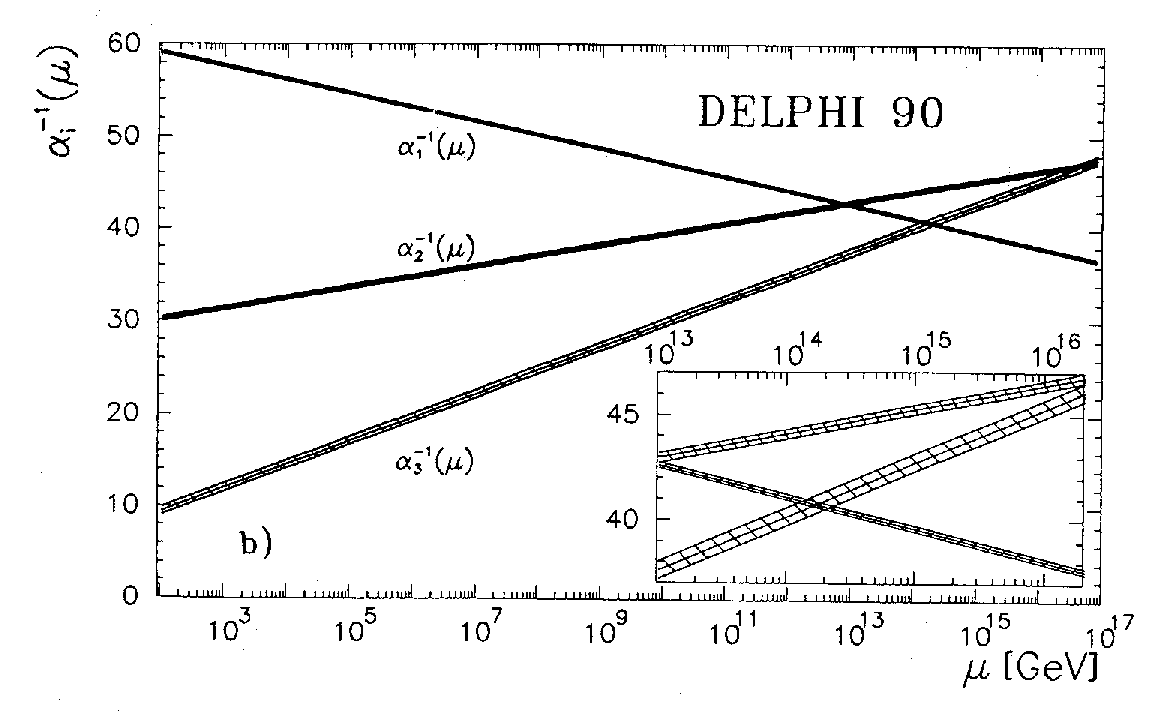
\includegraphics[width=0.49\textwidth]{figures/theory/running_couplings_SM}
      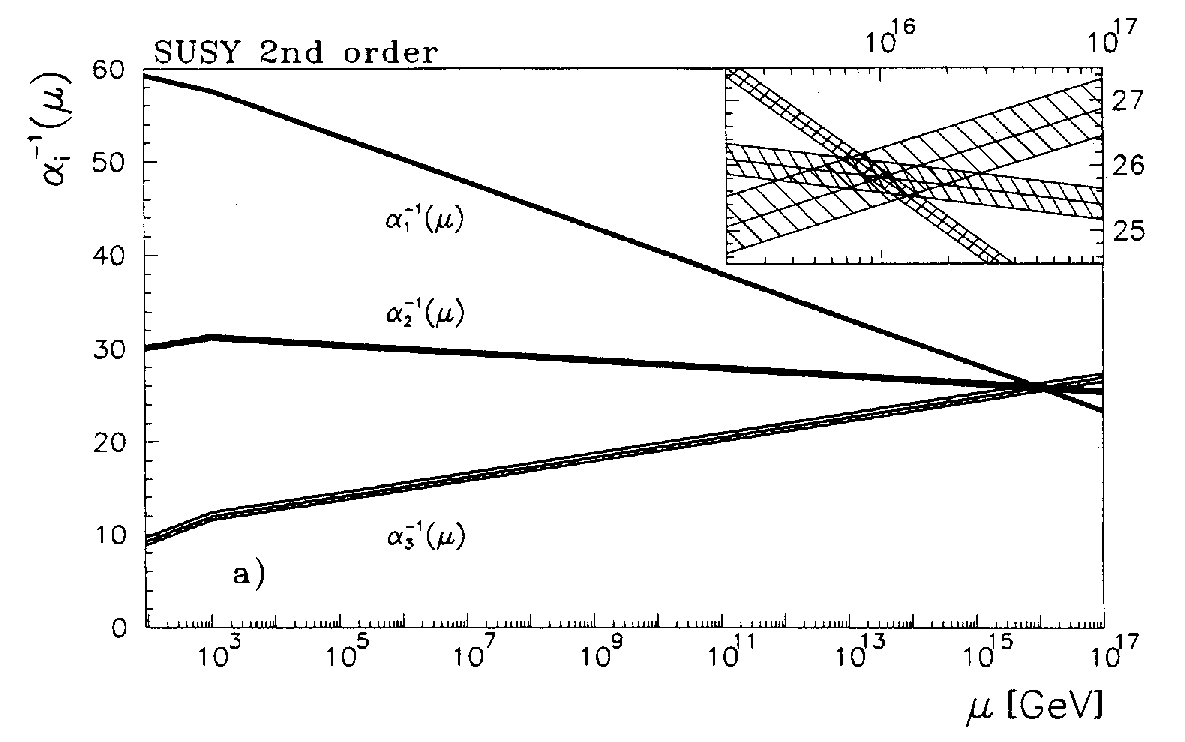
\includegraphics[width=0.49\textwidth]{figures/theory/running_couplings_MSSM}
  \caption{The running of the gauge couplings in the Standard Model (left) and in the minimal supersymmetric extension of the SM (right). Taken from~\cite{bib:Unification}.}  
  \label{fig:Unification}
\end{figure}

Besides these arguments, SUSY can also provide an answer to the problem of non-visible matter in the universe.
If the conservation of the so-called R-parity is required, the lightest supersymmetric particle (LSP) is stable.
If this particle is only weakly interacting, it can serve as a good candidate to explain fully or partially the sources of the relic density. 
R-parity is a multiplicative quantum number with 
\begin{equation}
\begin{aligned}
P_R & =  1 \qquad &&\text{SM particles}\\
P_R & = -1 &&\text{SUSY particles}.
\end{aligned}
\end{equation}
If R-parity is conserved, only terms are allowed in the Lagrangian density, that contain an even number of supersymmetric particles.
Therefore, no single SUSY particle can decay into only SM particles and thus, the LSP is stable.
The following discussions are restricted to R-parity conserving supersymmetric models.



\section{The MSSM}
\label{sec:MSSM}
The supersymmetric extension of the Standard Model with a minimal particle content is called the Minimal Supersymmetric Standard Model (MSSM).
In the following section, the particle content of the MSSM is introduced.

\subsection{The particle content of the MSSM}
In $\mathcal{N}=1$ supersymmetry, every SM particle has exactly one supersymmetric partner particle, which leads to a doubling of the particle content in the MSSM with respect to the SM\footnote{The supersymmetric partner particles of the fermions are called sfermions, whereas the partner particles of the gauge (Higgs) bosons are referred to as gauginos (higgsinos).}.
Additionally, it is necessary to introduce a second Higgs doublet to ensure the holomorphicity of the superpotential in the presence of mass terms for the up-type particles.
Furthermore, the MSSM only stays free from anomalies if there is a further Higgs doublet~\cite{bib:SUSYPrimer}.
This leads to the fact, that in the MSSM, there are five Higgs bosons instead of only one as in the SM.

\renewcommand{\arraystretch}{1.5}
\begin{table}[!b]
\centering
\caption{Chiral supermultiplets in the MSSM.}
\label{tab:chiral_multiplets}
\makebox[0.99\textwidth]{
\begin{tabular}{l|c|c|c}
\multicolumn{4}{c}{} \\
\toprule
                     &   spin 0                                     & spin $\frac{1}{2}$              & $SU(3)_C,\ SU(2)_L,\ U(1)_Y$\\ 
\midrule
   squarks/quarks    & $\left(\tilde{u}_L,\tilde{d}_L \right)$      & $\left(u_L,d_L\right)$           & $\mathbf{3},\ \mathbf{2},\ +\frac{1}{3}$\\ \cline{2-4}  
                     & $\tilde{\bar{u}}_L = \tilde{u}_R^{\dagger} $   & $\bar{u}_L = (u_R)^c$            & $\mathbf{\bar{3}},\ \mathbf{1},\ -\frac{4}{3}$\\ \cline{2-4}  
                     & $\tilde{\bar{d}}_L = \tilde{d}_R^{\dagger}$    & $\bar{d}_L = (d_R)^c$            & $\mathbf{\bar{3}},\ \mathbf{1},\ +\frac{2}{3}$\\ 
\midrule
   sleptons/leptons  & $\left(\tilde{\nu}_{eL},\tilde{e}_L\right)$   & $\left(\nu_{eL},e_L\right)$      & $\mathbf{1},\ \mathbf{2},\ -1$\\ \cline{2-4} 
                     & $\tilde{\bar{e}}_L = \tilde{e}_R^{\dagger}$    & $\bar{e}_L = (e_R)^c$            & $\mathbf{\bar{1}},\ \mathbf{1},\ +2$\\ 
\midrule
   Higgs/higgsinos   & $\left(H_u^+,H_u^0\right)$        & $\left(\tilde{H}_u^+,\tilde{H}_u^0\right)$   & $\mathbf{1},\ \mathbf{2},\ +1$\\ \cline{2-4}
                     & $\left(H_d^0,H_d^-\right)$        & $\left(\tilde{H}_d^0,\tilde{H}_d^-\right)$   & $\mathbf{1},\ \mathbf{2},\ -1$ \\ 
\bottomrule
\multicolumn{4}{c}{} 
\end{tabular}}
\end{table}  
\renewcommand{\arraystretch}{1.5}
\begin{table}[!b]
\centering
\caption{Vector supermultiplets in the MSSM.}
\label{tab:vector_multiplets}
\makebox[0.99\textwidth]{
\begin{tabular}{l|c|c|c}
\multicolumn{4}{c}{} \\
\toprule
                      &   spin $\frac{1}{2}$                                  & spin 1                 & $SU(3)_C,\ SU(2)_L,\ U(1)_Y$\\ 
\midrule
   gluinos/gluons     & $\tilde{g}$                       & $g$                 & $\mathbf{8},\ \mathbf{1},\ 0$\\ 
\midrule
   winos/$W$-bosons   & $\tilde{W}^{\pm},\ \tilde{W}^0$  & $W^{\pm},\ W^0$     & $\mathbf{1},\ \mathbf{3},\ 0$\\
\midrule
   bino/$B$-boson     & $\tilde{B}$                      & $B$                 & $\mathbf{1},\ \mathbf{1},\ 0$ \\  
\bottomrule
\multicolumn{4}{c}{}
\end{tabular}}
\end{table} 
In supersymmetry, all particles and their partner particles are described by so-called supermultiplets.
Since the generators of the gauge group commute with the generators of supersymmetry, all particles within one supermultiplet have same quantum numbers, besides the spin.
In a renormalisable theory, there are two different types of supermultiplets: chiral multiplets, which contain a two-component Weyl spinor describing the fermionic degrees of freedom and a complex scalar field for the bosonic degrees of freedom; vector multiplets containing a vector field and a two-component Weyl spinor.
The complete particle content of the MSSM is depicted in Tables~\ref{tab:chiral_multiplets} and~\ref{tab:vector_multiplets}. 
Since in supersymmetric theories only left-handed Weyl spinors appear in the Lagrangian density, the right-handed particles are described as charge conjugated spinors of the left-handed spinors.





\subsection{The Lagrangian density of the MSSM}
\label{sec:Lagrange_MSSM}
In the following, only the most important parts of the MSSM Lagrangian density will be described.
For a complete description of the Lagrangian density, the reader is again referred to~\cite{bib:Drees_2004}.

\subsubsection*{The superpotential}
The superpotential of the MSSM contains the self interaction terms of the Higgs bosons and generates the interaction terms of the Higgs bosons with the fermions and their superpartners.
As already noted, it is very common to assume R-parity conservation.
Hence, no terms appear in the Lagrangian that would violate lepton or baryon number conservation and the lightest supersymmetric particle is stable.
Thus, all possible terms are
\begin{equation}
\label{eq:SPMSSM}
 W_{\text{MSSM}} = \mu H_u \cdot H_d - Y_u^{ij} H_u \cdot Q_L^i u_R^{c\,j} + Y_d^{ij} H_d \cdot Q_L^i d_R^{\,c\,j} + Y_e^{ij} H_d \cdot L_L^i e_R^{c\,j},
\end{equation}
with the dot product defined as in~\cite{bib:Aitchison_2005} 
\begin{equation}
 A \cdot B = \epsilon^{\alpha\beta} A_{\alpha} B_{\beta} = A_1 B_2 - A_2 B_1.
\end{equation}

\subsubsection*{The soft-breaking Lagrangian density}
Since supersymmetry is broken, explicit SUSY breaking terms are added to the Lagrangian density.
In order not to introduce new sources of quadratic divergencies, only bilinear and trilinear terms appear in the soft-breaking Lagrangian
\begin{equation}
 \begin{split}
  - \mathcal{L}^{MSSM}_{soft} =\,& m_{H_u}^2 H_u^{\dagger} \cdot H_u +m_{H_d}^2 H_d^{\dagger} \cdot H_d + \left(B\mu\, H_u \cdot H_d + h.c.\right) \\
  & + m_{\tilde{Q}\,ij}^2 \tilde{Q}_{L\,i}^{\dagger} \cdot \tilde{Q}_{L\,j}+ m_{\tilde{u}\,ij}^2 \tilde{u}_{R\,i}^{c\,\dagger} \cdot \tilde{u}_{R\,j}^c
+ m_{\tilde{d}\,ij}^2 \tilde{d}_{R\,i}^{\,c\,\dagger} \cdot \tilde{d}_{R\,j}^{\,c}\\
& + m_{\tilde{L}\,ij}^2 \tilde{L}_{L\,i}^{\dagger} \cdot \tilde{L}_{L\,j}+ m_{\tilde{e}\,ij}^2 \tilde{e}_{R\,i}^{\,c\,\dagger} \cdot \tilde{e}_{R\,j}^{\,c}\\
& +\left(- \left( A_u Y_u \right)_{ij} H_u \cdot \tilde{Q}_{L\,i} \tilde{u}_{R\,j}^c +\left( A_d Y_d \right)_{ij} H_d \cdot \tilde{Q}_{L\,i} \tilde{d}_{R\,j}^{\,c} \right.\\
& \left. +\left( A_e Y_e \right)_{ij} H_d \cdot \tilde{L}_{L\,i} \tilde{e}_{R\,j}^{\,c} + h.c. \right)\\
& + \left(M_1 \tilde{B} \tilde{B} + M_2 \tilde{W}_a \tilde{W}_a + M_3 \tilde{g}_i \tilde{g}_i + h.c \right)
 \end{split}
\label{eq:SoftTerms}
\end{equation}
The first line contains mass terms for the Higgs bosons, the second and third line for the sfermions.
In the fourth and fifth line the trilinear couplings between the Higgs bosons and the sfermions appear.
Finally, the last line gives rise to mass terms for the gauginos (gluinos, winos, bino).

Because of the soft-breaking terms, the MSSM contains more than 100 free parameters.
Constraining the MSSM is thus a difficult task and usually in experimental particle physics, constrained versions of the MSSM or assumptions at the GUT scale are used to report the impact of searches on SUSY. 
In the following a short introduction of the phenomenological MSSM is given.
With its reduced parameter space, it allows to elaborate on long-lived particles in the MSSM in a much easier way.

\subsection{The phenomenological MSSM}
\label{subsec:pMSSM}
The phenomenological MSSM (pMSSM) imposes constraints that are reasonable in the sense that the pMSSM fulfils current observations and still keeps the phenomenological variety of the MSSM~\cite{bib:pMSSM}.
The following assumptions are imposed (in~\cite{bib:pMSSM} more detailed information about these assumptions can be found):
\begin{itemize}
\item No new sources of CP violation,
\item No flavour changing neutral currents,
\item First and second generation universality.
\end{itemize}
These assumption reduce the number of SUSY parameters to only 19.
The remaining free parameters are the following:
\begin{itemize}
\item $\tan \beta$ (the ratio of the vacuum expectation values of the two Higgs doublets)
\item $M_A$ (the mass of the pseudo-scalar Higgs boson)  
\item $\mu$ (the Higgs mass parameter)
\item $M_1$,$M_2$,$M_3$ (bino, wino and gluino mass parameters, respectively)
\item $m_{\tilde{q}}$, $m_{\tilde{l}}$, $m_{\tilde{u}}$, $m_{\tilde{d}}$ and $m_{\tilde{e}}$ (the first and second generation mass parameters)
\item  $m_{\tilde{Q}}$, $m_{\tilde{L}}$, $m_{\tilde{t}}$, $m_{\tilde{b}}$ and $m_{\tilde{\tau}}$ (the third generation mass parameters)
\item $A_t$, $A_b$ and $A_{\tau}$ (third generation trilinear couplings).
\end{itemize}

\section{Supersymmetry breaking}
As already noted, the mechanism of supersymmetry breaking is unknown.
There exist, however, several ideas how to spontaneously break supersymmetry.
All mechanisms have in common that they need to happen at high energies in a hidden sector.
``Messenger'' particles are introduced which mediate the breaking to the TeV scale.
This, however, implies that supersymmetry breaking is a question of extraordinary high energies and one can parametrise the breaking by the soft breaking terms introduced in Section~\ref{sec:Lagrange_MSSM}.

The most popular breaking mediation mechanisms are gravity-mediated supersymmetry breaking~\cite{bib:GravityMediation} and gauge-mediated supersymmetry breaking~\cite{bib:GaugeMediation}.

\chapter{Long-lived particles in the MSSM}
\label{ch:Longlived_Particles}
There are various mechanisms how particles can be long-lived, such as small couplings or (almost) conserved quantum numbers.
For a comprehensive review, the reader is referred to~\cite{bib:LonglivedParticles_Overview}.

In this thesis, the focus is set on particles that have a long lifetime due to a small decay phase space. 
A phase space suppression is possible when the mass splitting between the decaying particle and one of the decay products is very small.
In Part~\ref{part:analysis}, a search for highly ionising, short tracks is presented.
This search is motivated by long-lived charginos, that are nearly mass-degenerate with the lightest supersymmetric particle, the neutralino.
The underlying mechanism of this mass-degeneracy in the MSSM will be addressed in the next paragraphs.

In the MSSM, the lightest chargino (\chipm) and the lightest neutralino (\chiO) can be almost mass-degenerate, if the wino mass parameter ($M_2$) is smaller than the bino ($M_1$) and higgsino ($\mu$) mass parameters.
This can be seen from the chargino and neutralino mass matrices.
The chargino mass matrix in the basis $\Psi^+_i= \left(-i \tilde{W}^+,\tilde{h}_u^+  \right)$ and \mbox{$\Psi^-_i= \left(-i \tilde{W}^-,\tilde{h}_d^-  \right)$} is given by 
\begin{flalign}
\label{eq:CharginoMassMatrix}
\mathcal{M}_{\Psi^{\pm}} = 
\begin{pmatrix} 
M_2    & g v_d                    \\
g v_u  & \mu                  
\end{pmatrix}.
\end{flalign} 
The mass eigenstates can be deduced with the help of orthogonal matrices $V$ and $U$, \mbox{$\chi^+_i=V_{ij}\Psi^+_j$} and \mbox{$\chi^-_i = U_{ij} \Psi^-_j$}.

The neutralino mass matrix in the basis  $\Psi_i^0= \left(-i\tilde{B},-i\tilde{W}^0,\tilde{h}_u^0,\tilde{h}_d^0\right)$ is
\begin{flalign}
\label{eq:NeutralinoMassMatrix}
\mathcal{M}_{\Psi^0} = 
\begin{pmatrix} 
M_1                     & 0                       & \frac{g'v_u}{\sqrt{2}}  & -\frac{g'v_d}{\sqrt{2}}  \\
0                       & M_2                     & -\frac{g v_u}{\sqrt{2}} & \frac{g v_d}{\sqrt{2}}   \\
\frac{g'v_u}{\sqrt{2}}  & -\frac{g v_u}{\sqrt{2}} & 0                       & -\mu                     \\
-\frac{g'v_d}{\sqrt{2}} & \frac{g v_d}{\sqrt{2}}  & -\mu                    &  0                      
\end{pmatrix}.
\end{flalign}
The mass matrix can be diagonalised with an orthogonal matrix $N$ leading to four different mass eigenstates of $\tilde{\chi}^0_i = N_{ij} \Psi_j^0  $.

It can be easily seen from the mass matrices~\eqref{eq:CharginoMassMatrix} and~\eqref{eq:NeutralinoMassMatrix}, that in first order approximation - neglecting the off-diagonal elements which are of electroweak strength - the lightest chargino and the lightest neutralino are both wino-like for $M_2 < M_1,\mu$ with a mass of $m_\chi \simeq M_2$. 
Thus, the mass difference between \chipm and \chiO is only determined by higher order corrections: radiative corrections as well as tree-level mixing with other states.\\

%The following expressions are approximate neutralino and chargino mass terms for $M_2 \mu > m_W^2 \sin 2\beta$ and $|M_2 \pm \mu|$, $|M_1 \pm \mu| \gg m_Z$ (taken from~\cite{bib:PAS:CMS:pMSSM_2013})
%\begin{align}
%\label{eq:gaugino_masses}
%\begin{split}
%m_{\tilde{B}}    &\simeq  M_1   + \frac{m_Z^2 \left( M_1 + \mu \sin 2\beta  \right) \sin^2 \theta_W}{M_1^2 - \mu^2} \\
%m_{\tilde{W}}    &\simeq  M_2   + \frac{m_Z^2 \left( M_2 + \mu \sin 2\beta  \right) \cos^2 \theta_W}{M_2^2 - \mu^2} \\
%m_{\tilde{H}_1^0} &\simeq  |\mu| + \frac{m_Z^2 \left( 1 - \sin 2\beta \right) \left( \mu + M_2 \sin^2 \theta_W + M_1 \cos^2 \theta_W \right) sqn\left(\mu \right)}{2 \left(\mu +M_2 \right)\left(\mu +M_1 \right)} \\
%m_{\tilde{H}_2^0} &\simeq  |\mu| + \frac{m_Z^2 \left( 1 + \sin 2\beta \right) \left( \mu - M_2 \sin^2 \theta_W - M_1 \cos^2 \theta_W \right) sqn\left(\mu \right)}{2 \left(\mu -M_2 \right)\left(\mu -M_1 \right)} 
%\end{split}
%\end{align}
%\begin{align}
%\label{eq:chargino_masses}
%\begin{split}
%m_{\tilde{W}^{\pm}} &\simeq  M_2  + m_W^2 \left[ \frac{M_2 + \mu \sin 2\beta}{M_2^2 - \mu^2} \right]\\
%m_{\tilde{H^{\pm}}} &\simeq  |\mu|  + m_W^2 sgn\left( \mu \right) \left[ \frac{\mu + M_2 \sin 2\beta}{\mu^2 - M_2^2} \right]
%\end{split}
%\end{align}
%It is obvious from Eqs.~\ref{eq:gaugino_masses} and~\ref{eq:chargino_masses}, that if $M_2 < M_1,\, |\mu|$, the lightest neutralino state is wino-like and is fully mass-degenerate on tree level with the lightest chargino.


Furthermore, recent analyses of the pMSSM parameter space~\cite{bib:pMSSMScan_2013,bib:pMSSMScan_2012} show, that models with almost pure wino-like neutralinos as LSPs mostly come along with wino-like charginos being the next-to lightest supersymmetric particle (NLSP).
In~\cite{bib:pMSSMScan_2013}, a parameter scan in the pMSSM parameter space is performed, flat in the 19 different SUSY parameters.
Afterwards, the generated 3 million pMSSM models are confronted with theoretical constraints as well as experimental observations.
Theoretical constraints are \eg requiring stable vacua and no colour- or charge breaking minima.
Furthermore, the agreement with precision electroweak data, heavy flavour physics and collider results from LEP, Tevatron and LHC is required.
The accordance with relic density data is only implemented as an upper bound.
Phenomenological MSSM models that survive these constraints and have a wino-like neutralino as lightest supersymmetric particle, do frequently contain  a metastable chargino.
In a fraction of $\sim 25\%$ of these models, the metastable chargino decays inside the tracker, calorimeter or muon chamber.
The mass splitting between chargino and neutralino in these scenarios is typically of the order of $\sim160\mev$~\cite{bib:pMSSMScan_2013}.

Furthermore, a study has been performed within~\cite{bib:CMS:DT_8TeV} which interpretes the results of various beyond Standard Model searches in terms of the fraction of excluded parameter points in the pMSSM.
This study shows, that lifetimes between $1\cm \lesssim c\tau \lesssim 30\cm$ could not yet been accessed by any of the existing searches (cf. Fig.~\ref{fig:pMSSMplot} in Section~\ref{sec:Motivation}).



\section{Previous searches and constraints from indirect searches}

Several previous searches are sensitive on SUSY scenarios with almost mass-degenerate wino-like charginos and neutralinos.
In the following an overview about these previous searches will be given.

\subsection*{Searches at LEP}
Several searches at LEP were hunting for almost mass-degenerate neutralino-chargino scenarios~\cite{bib:PreviousSearches_ALEPH,bib:PreviousSearches_OPAL,bib:PreviousSearches_DELPHI_2003,bib:PreviousSearches_DELPHI}.
These searches were looking for events with a high-energetic initial state radiated photon leading to missing energy in events with chargino-pair production and invisible decay products.
The excluded parameter regions by these searches can be found in~\cite{bib:LEP:SUSY_results} and are depicted in Fig.~\ref{fig:LEP}.
The searches were interpreted for $M_1$ and $M_2$ almost degenerate and with a large unified scalar mass $m_0$ leading to sneutrino masses larger than 500\gev. 
Charginos are excluded up to a mass of 92.4\gev~\cite{bib:LEP:SUSY_results}.
\begin{figure}[!h]
  \centering
      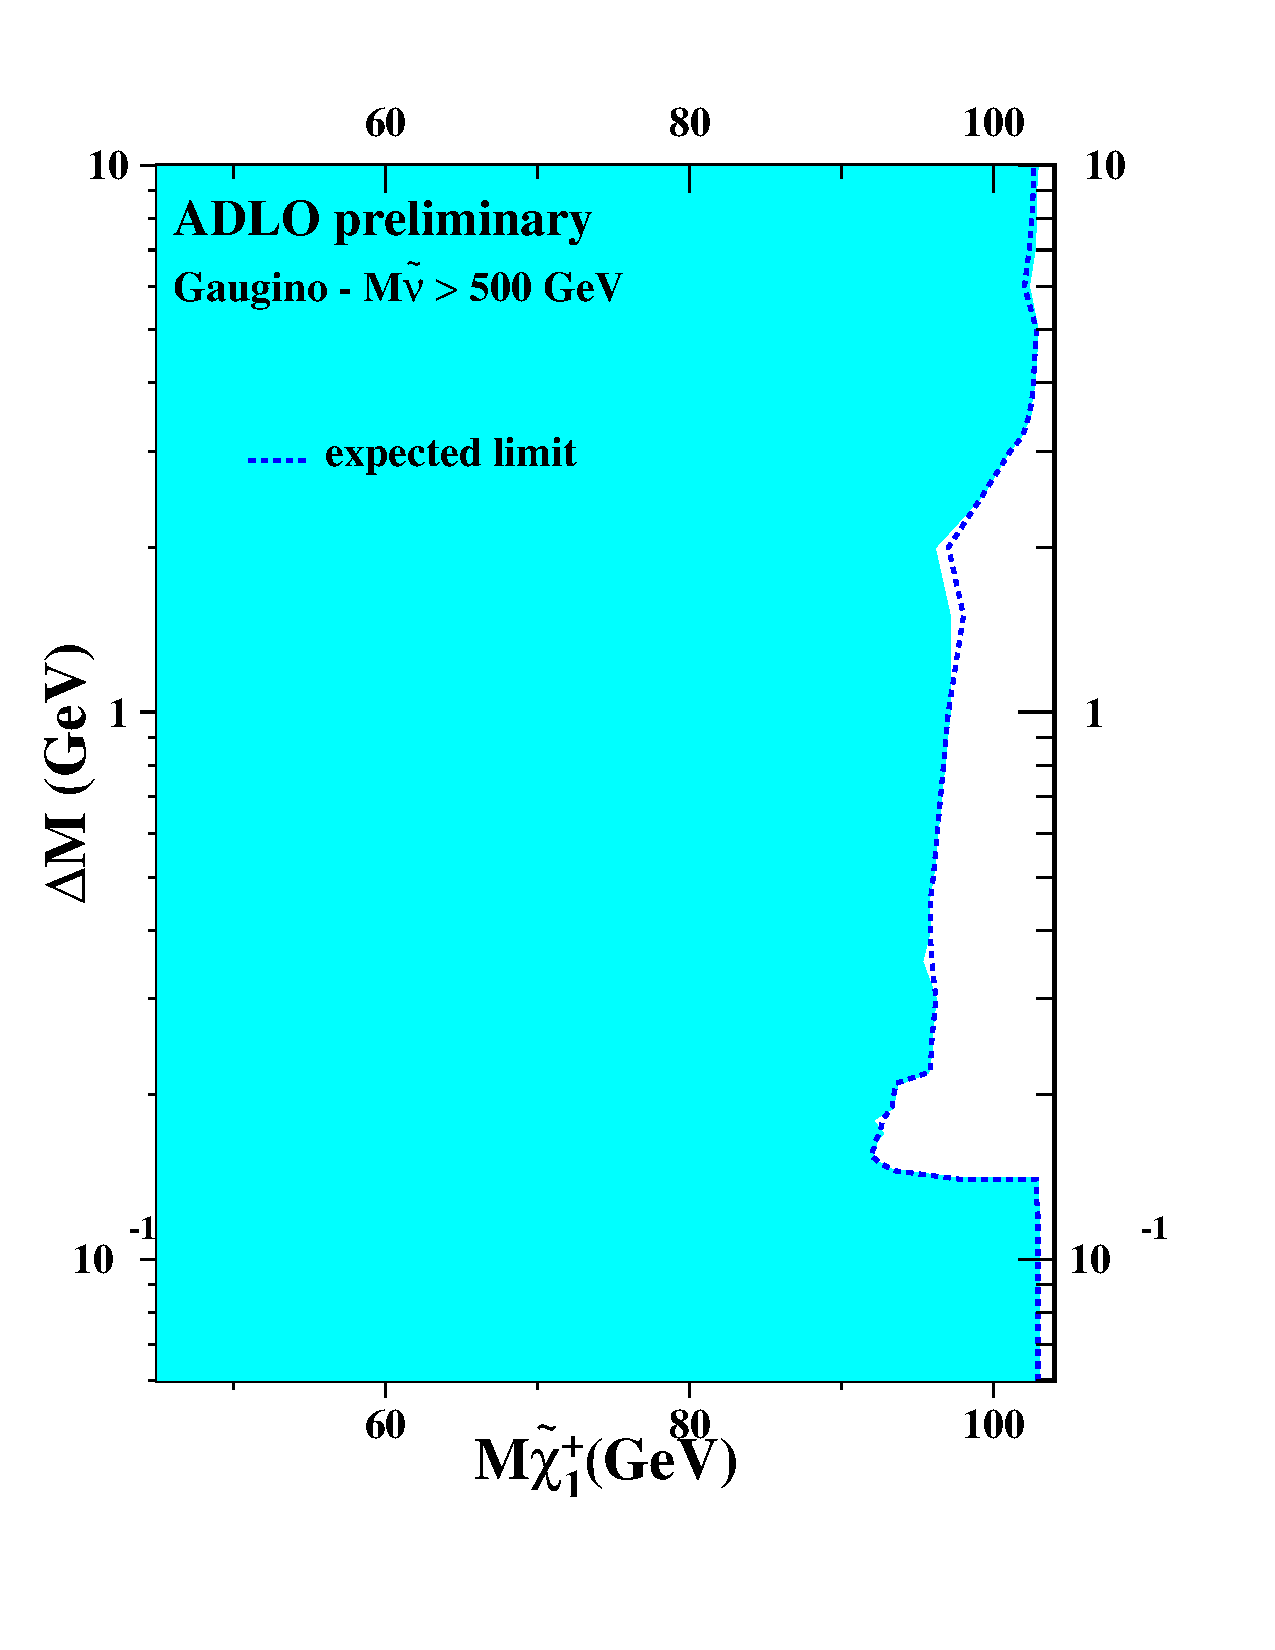
\includegraphics[width=0.45\textwidth]{figures/theory/mass_adlo_gaug_1.pdf}
  \caption{Observed and expected exclusion limits by LEP searches in the $m_{\chipm}-\Delta m \left( \chipm, \chiO \right)$ plane for almost degenerate $M_1$ and $M_2$ and a large unified scalar mass $m_0$. Taken from~\cite{bib:LEP:SUSY_results}.}  
  \label{fig:LEP}
\end{figure}

\subsection*{Searches at ATLAS at 7 and 8\tev}
At the ATLAS experiment at the LHC, searches for events with a disappearing track signature were performed at $\sqrt{s}=7\tev$~\cite{bib:PreviousSearches_Atlas_DT_7TeV} as well as at $\sqrt{s}=8\tev$~\cite{bib:PreviousSearches_Atlas_DT_8TeV}. 
Furthermore, a search for metastable particles with high ionisation losses was performed with $\sqrt{s}=8\tev$ data~\cite{bib:PreviousSearches_ATLAS_DEDX}.
These searches were interpreted within an anomaly-mediated supersymmetry breaking model~\cite{bib:Theory_AMSB_1998} with $\tan\beta=5$ and $\mu>0$.
The excluded parameter space by these searches is shown in Fig.~\ref{fig:ATLAS}.
Models with charginos down to lifetimes of 0.06\ns could be excluded.


\subsection*{Searches at CMS at 7 and 8\tev}
There are several searches at the CMS experiment at the LHC that are sensitive to long-lived wino-like charginos.
Among them is the search for long-lived charged particles~\cite{bib:CMS:HSCP_8TeV}, which searched for heavy particles with large energy deposits in the tracker at $\sqrt{s}=7\tev$  and $\sqrt{s}=8\tev$.
Furthermore, there is the search for disappearing tracks~\cite{bib:CMS:DT_8TeV} which analysed events with disappearing tracks in the tracker with respect to wino-like charginos almost mass-degenerate with the lightest neutralino.
This search was performed at the CMS experiment at a centre-of mass energy of $\sqrt{s}=8\tev$.
Since the latter search is more sensitive to shorter lifetime, only the exclusion limits derived by this search are shown in Fig.~\ref{fig:CMS}.
The disappearing track search by CMS shows a very similar sensitivity as the searches done at the ATLAS experiment.

\begin{figure}[!h]
  \centering
      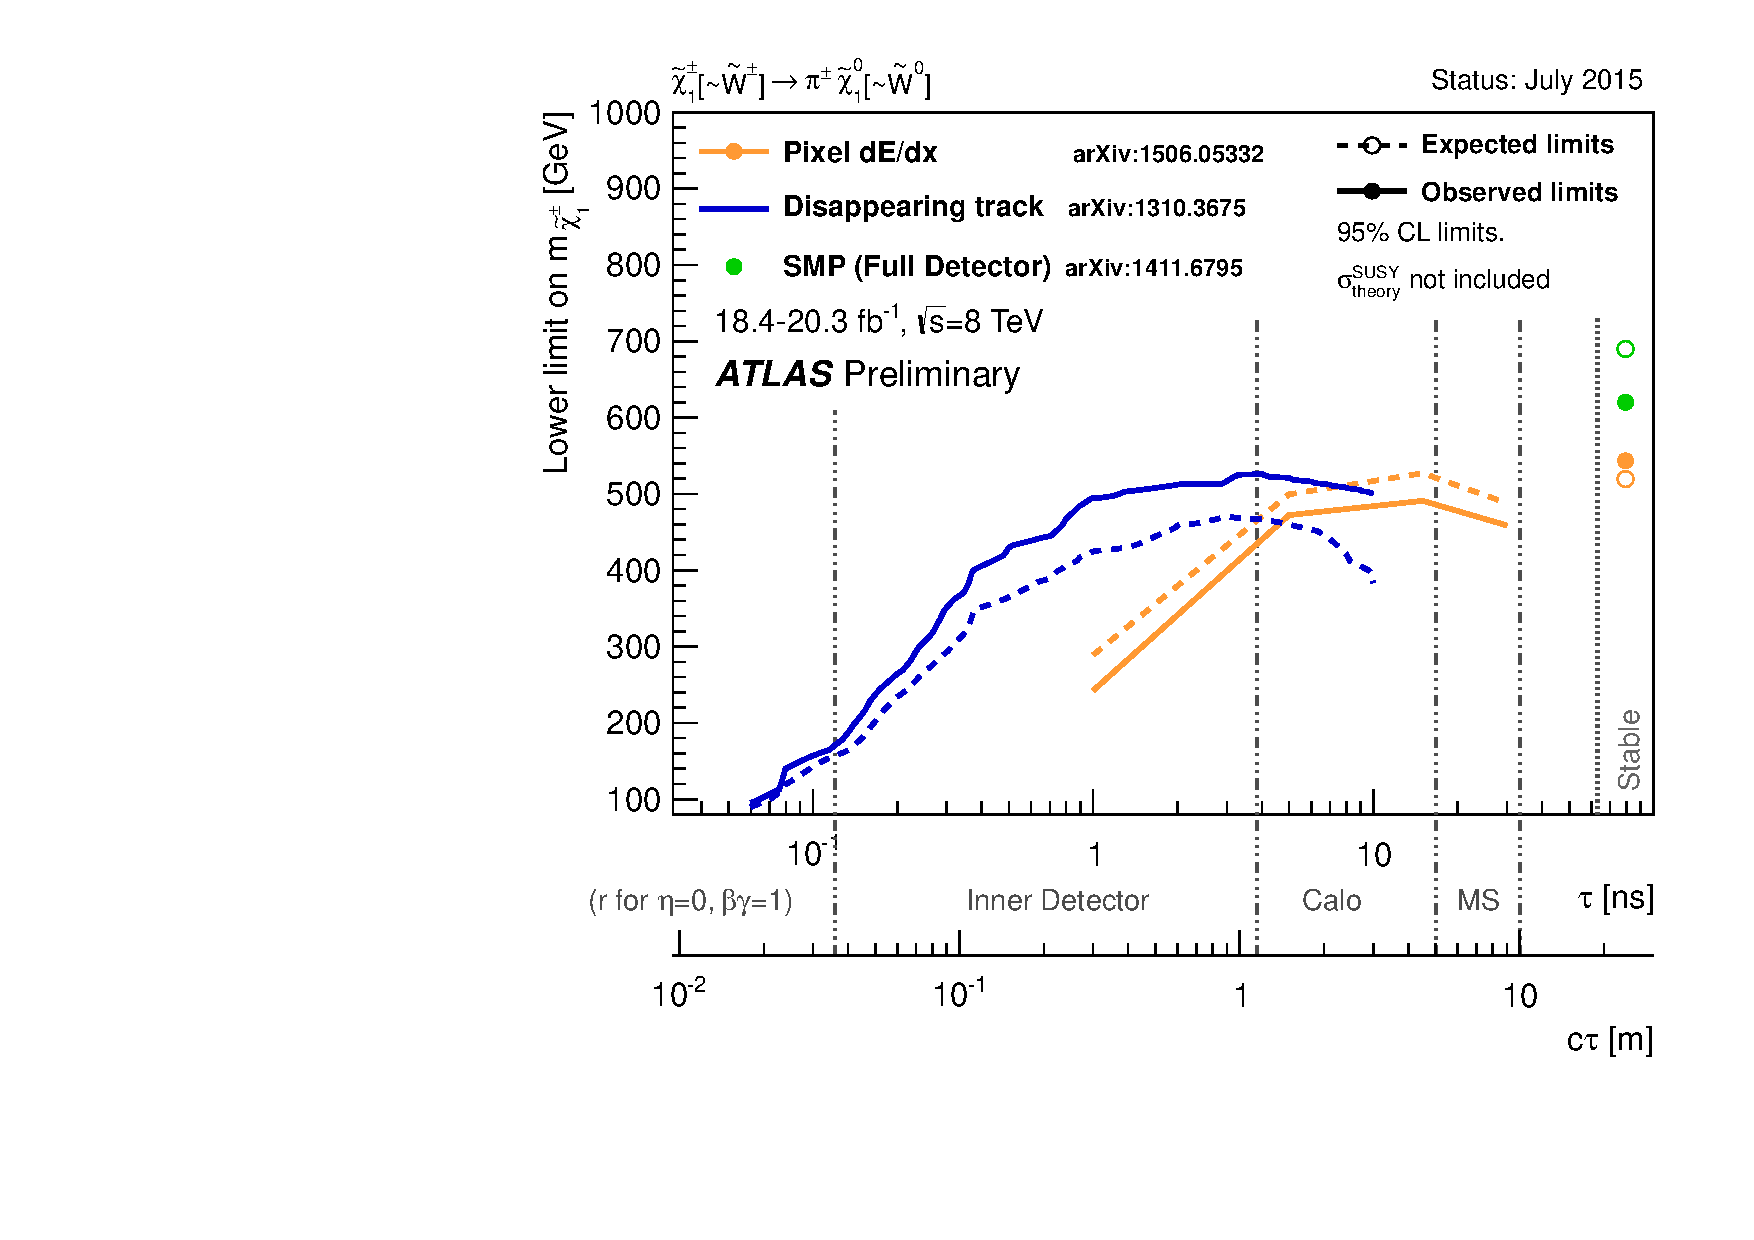
\includegraphics[width=0.54\textwidth]{figures/theory/ATLAS_SUSY_LLPChargino.pdf}
  \caption{Excluded parameter space by ATLAS searches in the $m_{\chipm}-\tau_{\chipm}$ plane for an AMSB model with $\tan\beta=5$ and $\mu>0$. Only chargino pair production is taken into account. The area below the curves is excluded. Taken from~\cite{bib:ATLAS_SUMMARYPLOTS}.}  
  \label{fig:ATLAS}
\end{figure}
\begin{figure}[!h]
  \centering
      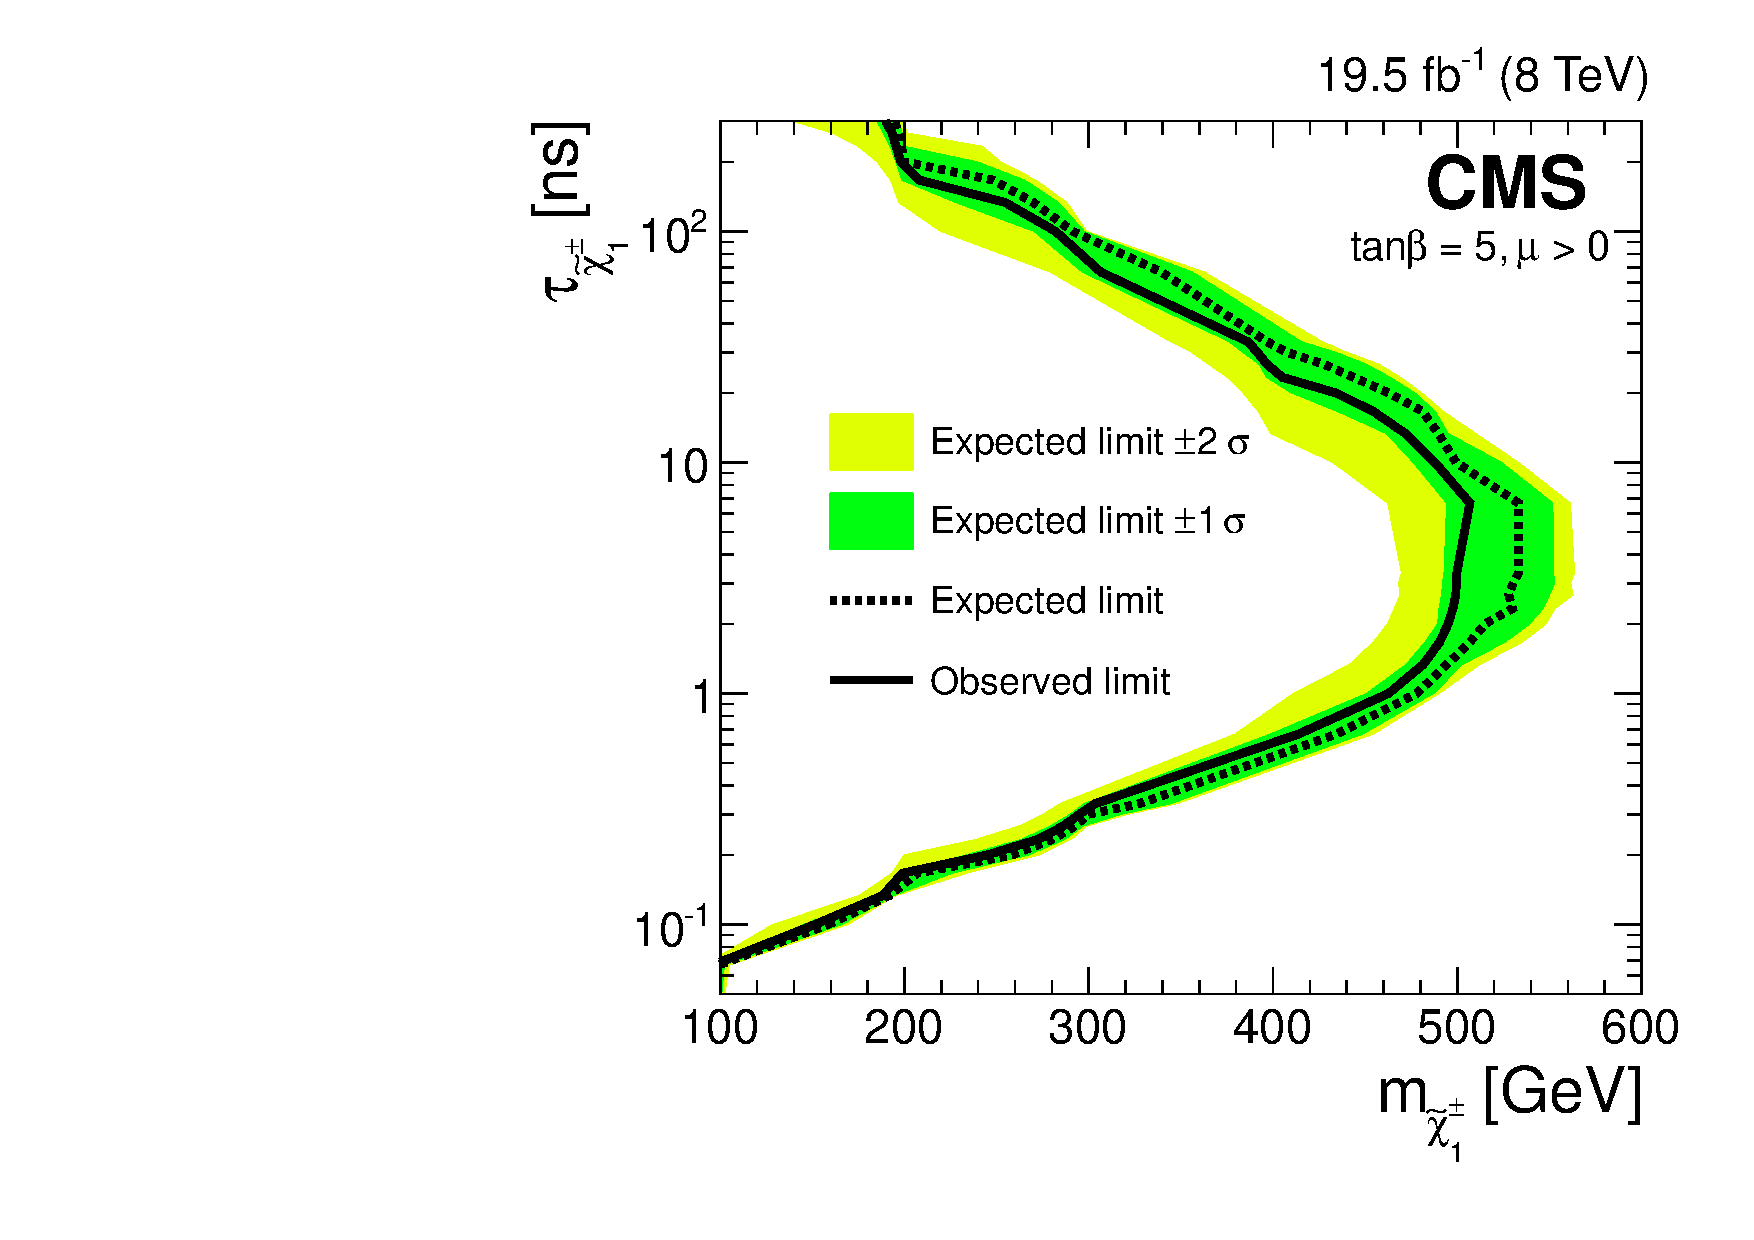
\includegraphics[width=0.54\textwidth]{figures/theory/lifetimeNs_vs_mass.pdf}
  \caption{Excluded parameter space by the Disappearing track search of CMS in the $\tau_{\chipm}-m_{\chipm}$ plane for wino-like charginos. The region left to the curve is excluded. Taken from~\cite{bib:CMS:DT_8TeV}.}  
  \label{fig:CMS}
\end{figure}

\subsection*{Indirect searches}
Finally, also results from indirect dark matter searches constrain the parameter region of SUSY models with wino-like charginos and neutralinos.
The most stringent limits are due to results by the Fermi Gamma-Ray Space Telescope (Fermi)~\cite{bib:Fermi} and the High Energy Spectroscopic System (H.E.S.S.)~\cite{bib:HESS}.

By the comparison of the observed gamma-ray signal to the theoretical prediction, Fermi sets upper limits on the dark matter annihilation cross-section considering six different decay channels~\cite{bib:Fermi_DM}.

H.E.S.S. sets upper limits on the DM annihilation cross section by the observation of the $\gamma$-ray line which is expected near the DM mass~\cite{bib:HESS_DM}.

Recent interpretations of the Fermi and H.E.S.S. data~\cite{bib:IndirectSearches_Fan_2013,bib:IndirectSearches_Cohen_2013,bib:IndirectSearches_Hryczuk_2014,bib:IndirectSearches_Beneke_2015} show that thermally produced wino-like neutralinos can only account for the full relic density for $\sim3.1\tev$~\cite{bib:IndirectSearches_Cohen_2013}, while DM masses between $1.6-3.0\tev$ are excluded by Fermi and H.E.S.S. observations.
Lower masses are still allowed, however, the neutralino cannot make up the full relic density.
%For scenarios with non-thermally produced neutralinos, the full mass region up to 3.1\tev is ruled out for scenarios where the wino-like neutralino is the only source of dark matter~\cite{bib:IndirectSearches_Cohen_2013}. 




% \part{Experimental setup/ Experiment and ... Experimental Setup: Collider, detector and algorithms } \label{sec:Detector}
% \section{LHC}
\section{CMS}
\section{Object reconstruction and particle identification}
\section{Event simulation}


%  \part{Measurement of the jet transverse-momentum resolution} \label{sec:resolution}
%  %%%%%%%%%%%%%%%%%%%%%%%%%%%%%%%%%%%%%%%%%%%%%%%%%%%%%%%%%%%%%%%%%%%%%%%%%%%%%%%%%%%%%%%%%%%%%%%%%%%%%%%%%%%%%%%%%%%%%%%%%%%%%%%%%%%%%%%%%%%%%%%%%%%%%%%%%%%%%%%%%%%%%%%%%%%%%%%%%%%%%%%%%%%%%%%%%%%%%%%%%%%%%%%%%%%%%%%%%%%%%%%%%%%%%%%%%%%
%%%%%%%%%%%%%%%%%%%%%%%%%%%%%%%%%%%%%%%%%%%%%%%%%%%%%%%%%%%%%%%%%%%%%%%%%%%%%%%%%%%%%%%%%%%%%%%%%%%%%%%%%%%%%%%%%%%%%%%%%%%%%%%%%%%%%%%%%%%%%%%%%%%%%%%%%%%%%%%%%%%%%%%%%%%%%%%%%%%%%%%%%%%%%%%%%%%%%%%%%%%%%%%%%%%%%%%%%%%%%%%%%%%%%%%%%%%
%%%%%%%%%%%%%%%%%%%%%%%%%%%%%%%%%%%%%%%%%%%%%%%%%%%%%%%%%%%%%%%%%%%%%%%%%%%%%%%%%%%%%%%%%%%%%%%%%%%%%%%%%%%%%%%%%%%%%%%%%%%%%%%%%%%%%%%%%%%%%%%%%%%%%%%%%%%%%%%%%%%%%%%%%%%%%%%%%%%%%%%%%%%%%%%%%%%%%%%%%%%%%%%%%%%%%%%%%%%%%%%%%%%%%%%%%%%
\chapter{Introduction}
\label{ch:Introduction}

The determination and quantification of the quality of the jet transverse momentum measurement is of crucial interest for many analyses with jet final states, 
\eg the measurement of the dijet cross section~\cite{bib:CMS:QCD_measurements} or $\ttbar$ production cross sections \cite{bib:CMS:TopCrossSection_8TeV}. 
Also searches for physics beyond the standard model with missing transverse momentum (\PTm) in the final state need a good knowledge of \PTm originating from wrongly measured jets \cite{}.
For analyses relying on information from simulation it is very important to correct the simulated resolution to the resolution actually present in data.
Therefore, scale factors will be presented to adjust the resolution in simulation to the resolution of the real detector.  
  
In the following sections, a data-based method to measure the jet \pt resolution in $\GAMJET$ events will be presented. 
A similar method was already accomplished in earlier analyses \cite{bib:CMS:JERCPaper_2011,bib:CMS-AN-2010-076,bib:CMS-AN-2010-141,bib:CMS-AN-2011-004} of 7\tev data.  
It is further developed here and applied to 8\tev data.

The method is based on the transverse momentum balance in the $\GAMJET$ system. 
It takes advantage of the high resolution of the electromagnetic calorimeter and hence the excellent measurement of the photon energy.
Without initial and final state radiation, the photon and the jet are balanced in the transverse plane. 
Thus, measuring the photon \pt with high accuracy leads to an estimate of the true jet transverse momentum offering a possibility to quantify the resolution of jet \pt measurements.


%%%%%%%%%%%%%%%%%%%%%%%%%%%%%%%%%%%%%%%%%%%%%%%%%%%%%%%%%%%%%%%%%%%%%%%%%%%%%%%%%%%%%%%%%%%%%%%%%%%%%%%%%%%%%%%%%%%%%%%%%%%%%%%%%%%%%%%%%%%%%%%%%%%%%%%%%%%%%%%%%%%%%%%%%%%%%%%%%%%%%%%%%%%%%%%%%%%%%%%%%%%%%%%%%%%%%%%%%%%%%%%%%%%%%%%%%%%
%%%%%%%%%%%%%%%%%%%%%%%%%%%%%%%%%%%%%%%%%%%%%%%%%%%%%%%%%%%%%%%%%%%%%%%%%%%%%%%%%%%%%%%%%%%%%%%%%%%%%%%%%%%%%%%%%%%%%%%%%%%%%%%%%%%%%%%%%%%%%%%%%%%%%%%%%%%%%%%%%%%%%%%%%%%%%%%%%%%%%%%%%%%%%%%%%%%%%%%%%%%%%%%%%%%%%%%%%%%%%%%%%%%%%%%%%%%
%%%%%%%%%%%%%%%%%%%%%%%%%%%%%%%%%%%%%%%%%%%%%%%%%%%%%%%%%%%%%%%%%%%%%%%%%%%%%%%%%%%%%%%%%%%%%%%%%%%%%%%%%%%%%%%%%%%%%%%%%%%%%%%%%%%%%%%%%%%%%%%%%%%%%%%%%%%%%%%%%%%%%%%%%%%%%%%%%%%%%%%%%%%%%%%%%%%%%%%%%%%%%%%%%%%%%%%%%%%%%%%%%%%%%%%%%%%
\chapter{General approach of the resolution measurement using photon+jet events}
\label{ch:GeneralApproach}

The jet transverse momentum resolution is defined as the standard deviation of the jet transverse momentum response distribution with the response 
defined as the ratio of the reconstructed to the true jet transverse momentum 
\begin{equation}\label{eq:responseFormula}
\mathcal{R} =  \frac{\pt^{\text{reco. jet}}}{\pt^{\text{true}}}.
\end{equation}
The jet transverse momentum resolution will be abbreviated JER throughout the following sections\footnote{This abbreviation is a historical relic from electron-position collider experiments where JER refered to jet energy resolution.}.

\mbox{Figure \ref{fig:TypicalResponse}} shows a typical response distribution for jets in the barrel region. 
\begin{figure}[t]
  \centering
      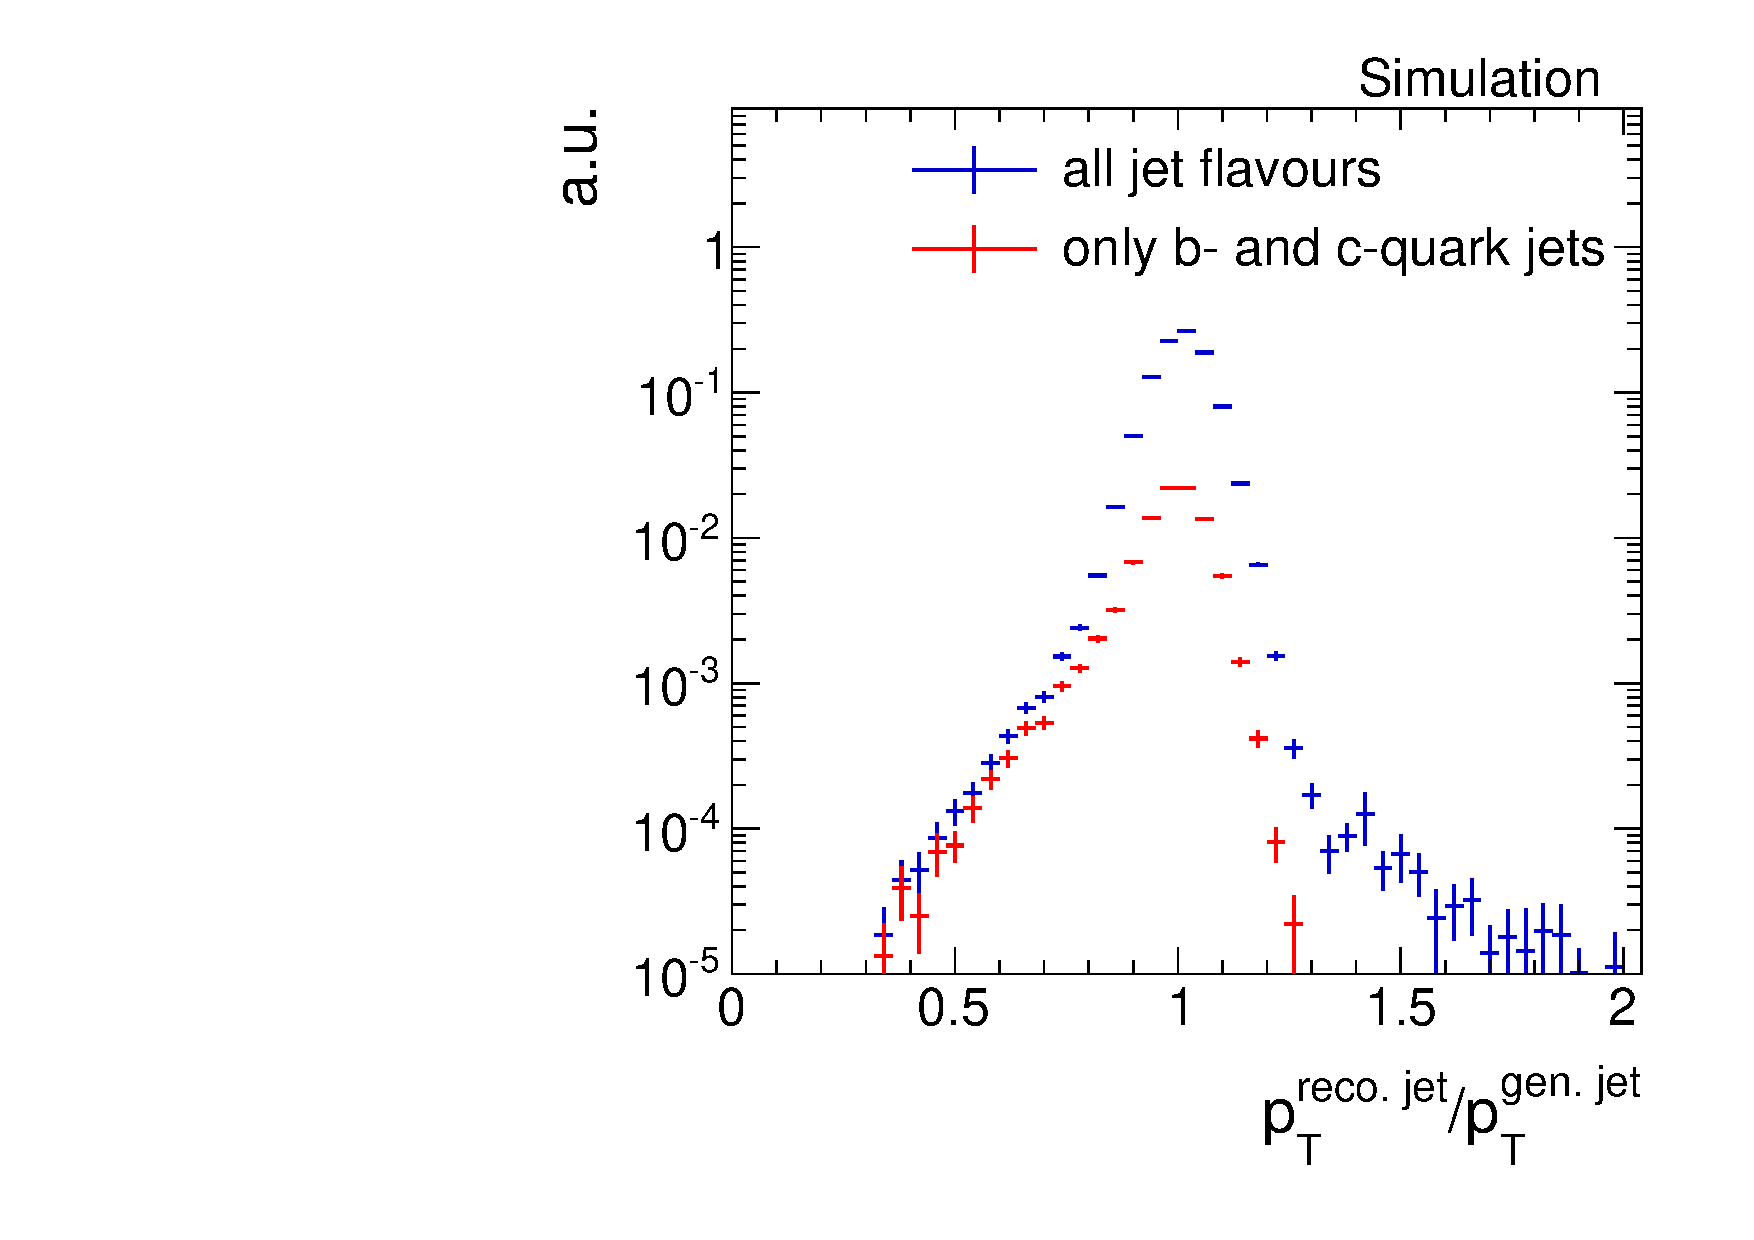
\includegraphics[width=0.49\textwidth]{figures/resolution/generalApproach/intrinsicExampleContributionofBCQuarks.pdf}
  \caption{Number of events over $\frac{\pt^{\text{reco. jet}}}{\pt^{\text{gen. jet}}}$ from a simulated $\GAMJET$ sample. 
           The black dots show the contribution by c- and b-quark jets where the left tail originating from semi-leptonic decays of heavy quarks can be seen.}  
  \label{fig:TypicalResponse}
\end{figure}
The core of the response distribution shows a Gaussian behavior whereas the tails deviate from that functional form.
Physical reasons for the low response tail are inter alia semi-leptonic decays of heavy quarks where the neutrino cannot be detected and the reconstructed transverse momentum of the jet is too small (see \mbox{Fig. \ref{fig:TypicalResponse}}). 
Some instrumental effects, such as a non-linear response of the calorimeter, inhomogeneities of the detector material and electronic noise can contribute to both tails, 
others, like dead calorimeter channels only contribute to the left tail. 
The resolution is therefore determined using only the core of the distribution to avoid the coverage of non-Gaussian tails.

Therefore, in this analysis note the resolution is defined as the standard deviation of the 99\% truncated response histogram devided by the mean of the histogram:

\begin{equation}\label{eq:resolutionFormula}
\text{JER} = \frac{\sigma_{99\%}}{\mu_{99\%}}.
\end{equation}

The determination of the 99\% range of the histogram is done in several steps. 
First the mean of the core is found via a Gaussian fit to the histogram in a 2$\sigma$ range \footnote{The 2$\sigma$ range is defined as the range [$\mu - 2\sigma$,$\mu + 2\sigma$].}. 
This procedure is done in three iteration steps.
Then, a symmetric interval around this mean is determined with its integral equal to 99\% of the integral of the full histogram. 

%The division by the mean is done to make the resolution measurement more insensitive to a variation of the jet energy scale (= mean of the response distribution)
%which has also an effect on the measured width of the distribution. 
%because response distributions with a scale smaller than one are typically narrower while distributions with scales larger than one are broader.

The evaluation of the response distribution as reconstructed over generated jet transverse momentum (\mbox{Eq.~\eqref{eq:responseFormula}})
is only possible for simulated events where generator information is accessible. 
A determination of the resolution in data, however, has to rely on a different approach.

The main idea of a resolution measurement using $\GAMJET$ events is based on the transverse momentum balance of the system and the excellent electromagnetic calorimeter resolution
(which was estimated between 1.1 \% and 2.6\% in the barrel region for photons for $\sqrt{s}= 7 \tev$ data \cite{bib:CMS:ECALresolution_7TeV} 
and is expected to be similar for $\sqrt{s}= 8 \tev$ data).

Several tree-level processes (\mbox{see Fig. \ref{fig:FeynmanDiagrams}}) lead to an event topology with one photon and one jet in the final state. 

\begin{figure}[htp]
  \centering

      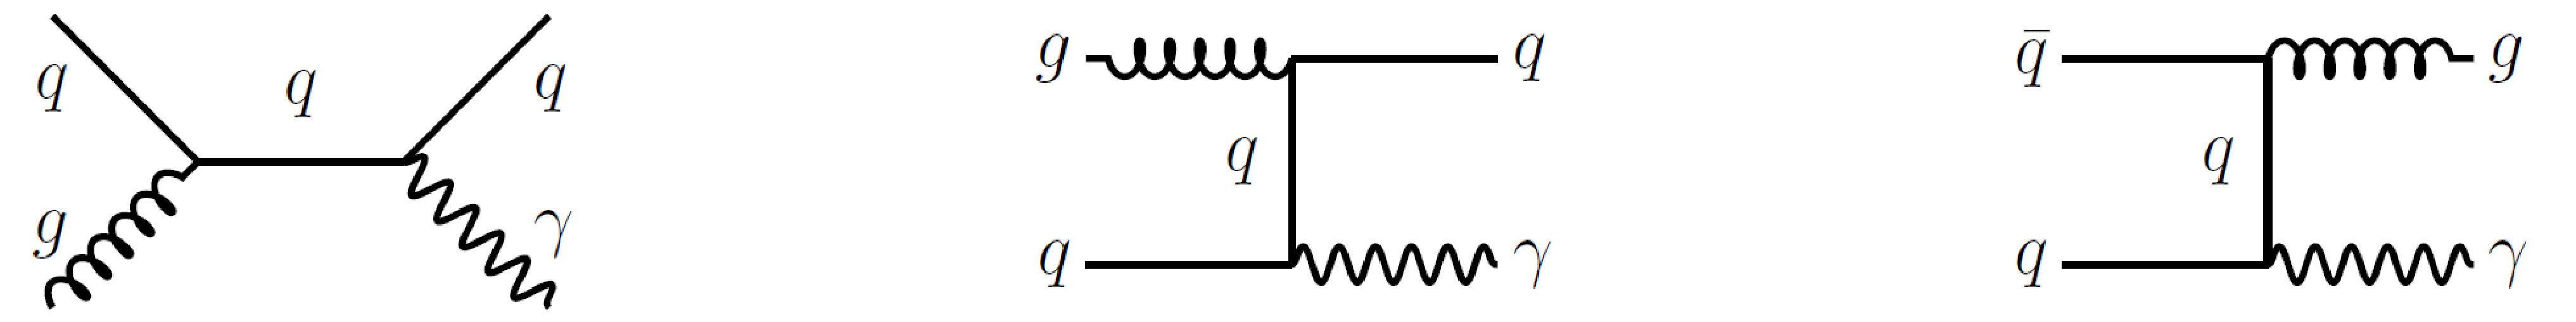
\includegraphics[width=0.99\textwidth]{figures/resolution/generalApproach/FeynmanDiagram.pdf}
 
 
  \caption{Tree-level Feynman diagrams of processes at the LHC in pp collisions with one photon and one jet in the final state.}  
  \label{fig:FeynmanDiagrams}
\end{figure}
Due to momentum conversation, the jet and the photon are back to back in the transverse plane, and therefore, $\vec{p}_{T}^{\gamma} = -\vec{p}_{T}^{\text{jet}}$. 
Because of the good resolution of the electromagnetic calorimeter, photon energies can be very well measured 
and thus can serve as an excellent estimator for the true jet energy.


Unfortunately, such clean events are very rare processes, and usually, the momentum balance is spoiled by initial and final state radiation, which lead to further jets in the event 
(see \mbox{Fig. \ref{fig:FeynmanDiagramsWithRadiation}}). 
However, in order to select events that are balanced to a large extent, a lower bound 
on the angular distance in the transverse plane between the photon and the jet with the highest transverse momentum (leading jet) is required ($\Delta\Phi>2.95\unit{rad}$). 

Additionally, the variable 

\begin{equation}\label{eq:alphaDef}
\alpha \doteq \frac{\pt^{\text{\nth{2} reco. jet}}}{\pt^{\gamma}}
\end{equation} 
is defined as a measure of further jet activity in an event. 
It is, however, not sufficient to require only an upper bound on $\alpha$. 
Instead, the jet energy resolution is measured in bins of $\alpha$ (with max($\alpha$) = 0.2), 
and the \mbox{extrapolated} value to zero further jet energy ($\alpha=0$) is taken as the measured resolution of the jet energy in the absence of further jets.


\begin{figure}[t]
  \centering

      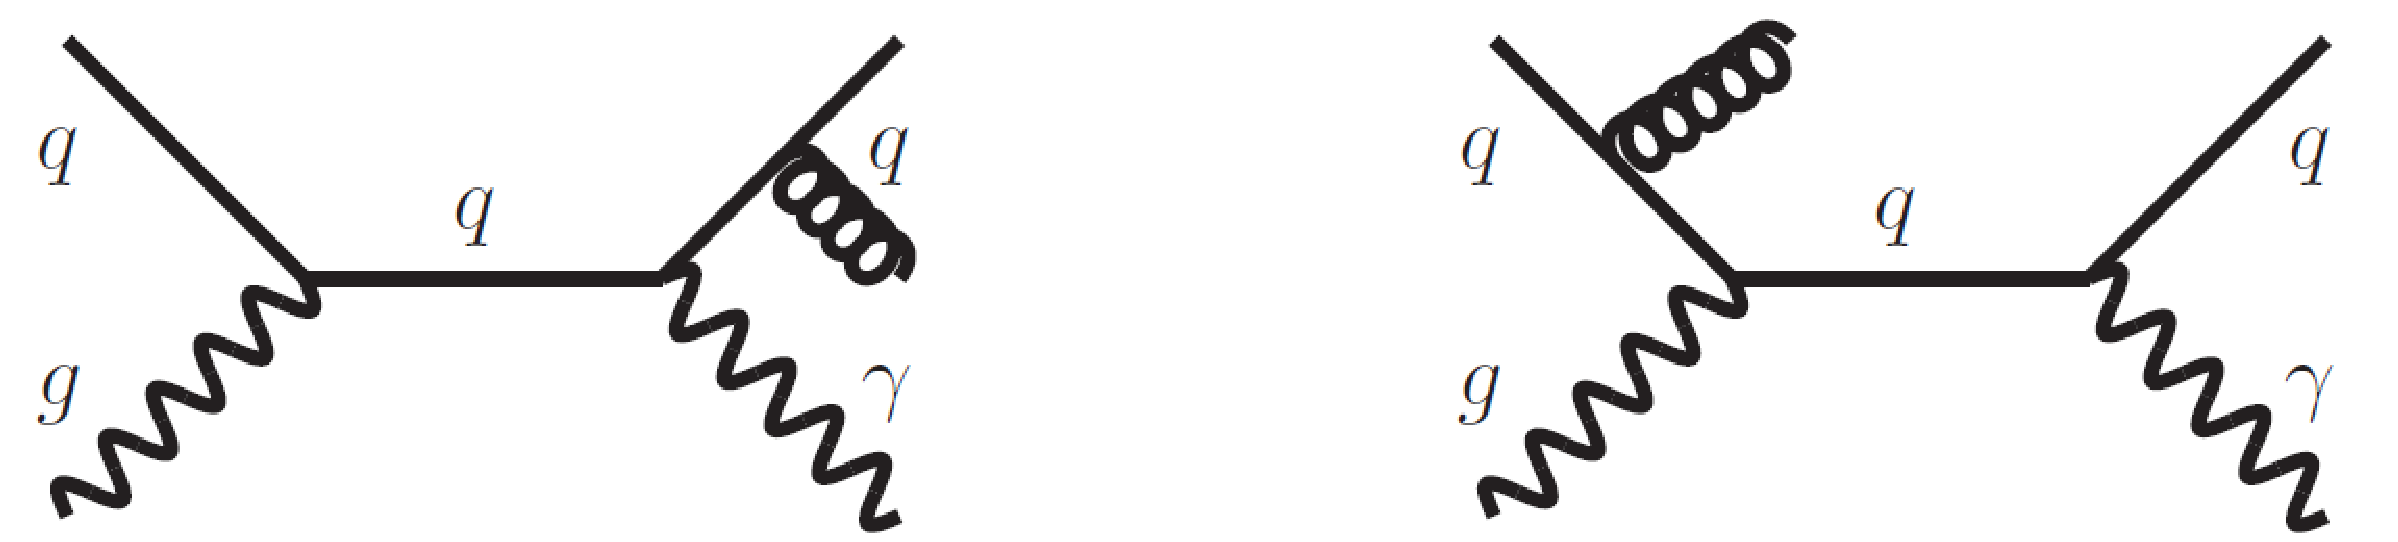
\includegraphics[width=0.60\textwidth]{figures/resolution/generalApproach/FeynmanDiagramsWithRadiation.pdf}
  
  \caption{Tree-level Feynman diagrams with initial and final state radiation.}  
  \label{fig:FeynmanDiagramsWithRadiation}
\end{figure}

Measuring the transverse momentum of the photon instead of taking the generator jet $p_{T}$ leads to the fact that the measured resolution consists out of two parts

\begin{equation}\label{eq:splitting}
\frac{\pt^{\text{reco. jet}}}{\pt^{\gamma}} = \underbrace{\frac{\pt^{\text{reco. jet}}}{\pt^{\text{gen. jet}}}}_{\text{intrinsic}} \cdot \underbrace{\frac{\pt^{\text{gen. jet}}}{\pt^{\gamma}}}_{\text{imbalance}}.
\end{equation}

The intrinsic part is the resolution of interest which is independent of further jets in the event whereas the imbalance is strongly dependent on $\alpha$.

To extract the intrinsic resolution out of the measured one, the residual imbalance $q^{\prime}$ (the imbalance at $\alpha = 0$) is subtracted from the total resolution in the 
limit of vanishing additional jet activity. 
As that information is only available from simulation, the measured resolution in data is corrected by the residual imbalance taken from the simulated data set.
%%%%%%%%%%%%%%%%%%%%%%%%%%%%%%%%%%%%%%%%%%%%%%%%%%%%%%%%%%%%%%%%%%%%%%%%%%%%%%%%%%%%%%%%%%%%%%%%%%%%%%%%%%%%%%%%%%%%%%%%%%%%%%%%%%%%%%%%%%%%%%%%%%%%%%%%%%%%%%%%%%%%%%%%%%%%%%%%%%%%%%%%%%%%%%%%%%%%%%%%%%%%%%%%%%%%%%%%%%%%%%%%%%%%%%%%%%%

%%%%%%%%%%%%%%%%%%%%%%%%%%%%%%%%%%%%%%%%%%%%%%%%%%%%%%%%%%%%%%%%%%%%%%%%%%%%%%%%%%%%%%%%%%%%%%%%%%%%%%%%%%%%%%%%%%%%%%%%%%%%%%%%%%%%%%%%%%%%%%%%%%%%%%%%%%%%%%%%%%%%%%%%%%%%%%%%%%%%%%%%%%%%%%%%%%%%%%%%%%%%%%%%%%%%%%%%%%%%%%%%%%%%%%%%%%%
%%%%%%%%%%%%%%%%%%%%%%%%%%%%%%%%%%%%%%%%%%%%%%%%%%%%%%%%%%%%%%%%%%%%%%%%%%%%%%%%%%%%%%%%%%%%%%%%%%%%%%%%%%%%%%%%%%%%%%%%%%%%%%%%%%%%%%%%%%%%%%%%%%%%%%%%%%%%%%%%%%%%%%%%%%%%%%%%%%%%%%%%%%%%%%%%%%%%%%%%%%%%%%%%%%%%%%%%%%%%%%%%%%%%%%%%%%%
\chapter{Datasets and event selection}

\begin{itemize}
\item  selection - take from AN
\end{itemize}

Pictures as root file available:
\begin{itemize}
\item BLA
\end{itemize}

Picture \textcolor{red}{NOT} as root file available:
\begin{itemize}
\item BLA
\end{itemize}
%%%%%%%%%%%%%%%%%%%%%%%%%%%%%%%%%%%%%%%%%%%%%%%%%%%%%%%%%%%%%%%%%%%%%%%%%%%%%%%%%%%%%%%%%%%%%%%%%%%%%%%%%%%%%%%%%%%%%%%%%%%%%%%%%%%%%%%%%%%%%%%%%%%%%%%%%%%%%%%%%%%%%%%%%%%%%%%%%%%%%%%%%%%%%%%%%%%%%%%%%%%%%%%%%%%%%%%%%%%%%%%%%%%%%%%%%%%

%%%%%%%%%%%%%%%%%%%%%%%%%%%%%%%%%%%%%%%%%%%%%%%%%%%%%%%%%%%%%%%%%%%%%%%%%%%%%%%%%%%%%%%%%%%%%%%%%%%%%%%%%%%%%%%%%%%%%%%%%%%%%%%%%%%%%%%%%%%%%%%%%%%%%%%%%%%%%%%%%%%%%%%%%%%%%%%%%%%%%%%%%%%%%%%%%%%%%%%%%%%%%%%%%%%%%%%%%%%%%%%%%%%%%%%%%%%
%%%%%%%%%%%%%%%%%%%%%%%%%%%%%%%%%%%%%%%%%%%%%%%%%%%%%%%%%%%%%%%%%%%%%%%%%%%%%%%%%%%%%%%%%%%%%%%%%%%%%%%%%%%%%%%%%%%%%%%%%%%%%%%%%%%%%%%%%%%%%%%%%%%%%%%%%%%%%%%%%%%%%%%%%%%%%%%%%%%%%%%%%%%%%%%%%%%%%%%%%%%%%%%%%%%%%%%%%%%%%%%%%%%%%%%%%%%
\chapter{Methodology of the measurement}

\begin{itemize}
\item Take from AN
\end{itemize}

Pictures as root file available:
\begin{itemize}
\item BLA
\end{itemize}

Picture \textcolor{red}{NOT} as root file available:
\begin{itemize}
\item BLA
\end{itemize}
%%%%%%%%%%%%%%%%%%%%%%%%%%%%%%%%%%%%%%%%%%%%%%%%%%%%%%%%%%%%%%%%%%%%%%%%%%%%%%%%%%%%%%%%%%%%%%%%%%%%%%%%%%%%%%%%%%%%%%%%%%%%%%%%%%%%%%%%%%%%%%%%%%%%%%%%%%%%%%%%%%%%%%%%%%%%%%%%%%%%%%%%%%%%%%%%%%%%%%%%%%%%%%%%%%%%%%%%%%%%%%%%%%%%%%%%%%%

%%%%%%%%%%%%%%%%%%%%%%%%%%%%%%%%%%%%%%%%%%%%%%%%%%%%%%%%%%%%%%%%%%%%%%%%%%%%%%%%%%%%%%%%%%%%%%%%%%%%%%%%%%%%%%%%%%%%%%%%%%%%%%%%%%%%%%%%%%%%%%%%%%%%%%%%%%%%%%%%%%%%%%%%%%%%%%%%%%%%%%%%%%%%%%%%%%%%%%%%%%%%%%%%%%%%%%%%%%%%%%%%%%%%%%%%%%%
%%%%%%%%%%%%%%%%%%%%%%%%%%%%%%%%%%%%%%%%%%%%%%%%%%%%%%%%%%%%%%%%%%%%%%%%%%%%%%%%%%%%%%%%%%%%%%%%%%%%%%%%%%%%%%%%%%%%%%%%%%%%%%%%%%%%%%%%%%%%%%%%%%%%%%%%%%%%%%%%%%%%%%%%%%%%%%%%%%%%%%%%%%%%%%%%%%%%%%%%%%%%%%%%%%%%%%%%%%%%%%%%%%%%%%%%%%%
\chapter{Systematic uncertainties}

\begin{itemize}
\item difficult to take from AN
\end{itemize}

Pictures as root file available:
\begin{itemize}
\item BLA
\end{itemize}

Picture \textcolor{red}{NOT} as root file available:
\begin{itemize}
\item BLA
\end{itemize}
%%%%%%%%%%%%%%%%%%%%%%%%%%%%%%%%%%%%%%%%%%%%%%%%%%%%%%%%%%%%%%%%%%%%%%%%%%%%%%%%%%%%%%%%%%%%%%%%%%%%%%%%%%%%%%%%%%%%%%%%%%%%%%%%%%%%%%%%%%%%%%%%%%%%%%%%%%%%%%%%%%%%%%%%%%%%%%%%%%%%%%%%%%%%%%%%%%%%%%%%%%%%%%%%%%%%%%%%%%%%%%%%%%%%%%%%%%%

%%%%%%%%%%%%%%%%%%%%%%%%%%%%%%%%%%%%%%%%%%%%%%%%%%%%%%%%%%%%%%%%%%%%%%%%%%%%%%%%%%%%%%%%%%%%%%%%%%%%%%%%%%%%%%%%%%%%%%%%%%%%%%%%%%%%%%%%%%%%%%%%%%%%%%%%%%%%%%%%%%%%%%%%%%%%%%%%%%%%%%%%%%%%%%%%%%%%%%%%%%%%%%%%%%%%%%%%%%%%%%%%%%%%%%%%%%%
%%%%%%%%%%%%%%%%%%%%%%%%%%%%%%%%%%%%%%%%%%%%%%%%%%%%%%%%%%%%%%%%%%%%%%%%%%%%%%%%%%%%%%%%%%%%%%%%%%%%%%%%%%%%%%%%%%%%%%%%%%%%%%%%%%%%%%%%%%%%%%%%%%%%%%%%%%%%%%%%%%%%%%%%%%%%%%%%%%%%%%%%%%%%%%%%%%%%%%%%%%%%%%%%%%%%%%%%%%%%%%%%%%%%%%%%%%%
\chapter{Results}

\begin{itemize}
\item THINK
\end{itemize}

Pictures as root file available:
\begin{itemize}
\item BLA
\end{itemize}

Picture \textcolor{red}{NOT} as root file available:
\begin{itemize}
\item BLA
\end{itemize}
%%%%%%%%%%%%%%%%%%%%%%%%%%%%%%%%%%%%%%%%%%%%%%%%%%%%%%%%%%%%%%%%%%%%%%%%%%%%%%%%%%%%%%%%%%%%%%%%%%%%%%%%%%%%%%%%%%%%%%%%%%%%%%%%%%%%%%%%%%%%%%%%%%%%%%%%%%%%%%%%%%%%%%%%%%%%%%%%%%%%%%%%%%%%%%%%%%%%%%%%%%%%%%%%%%%%%%%%%%%%%%%%%%%%%%%%%%%

%%%%%%%%%%%%%%%%%%%%%%%%%%%%%%%%%%%%%%%%%%%%%%%%%%%%%%%%%%%%%%%%%%%%%%%%%%%%%%%%%%%%%%%%%%%%%%%%%%%%%%%%%%%%%%%%%%%%%%%%%%%%%%%%%%%%%%%%%%%%%%%%%%%%%%%%%%%%%%%%%%%%%%%%%%%%%%%%%%%%%%%%%%%%%%%%%%%%%%%%%%%%%%%%%%%%%%%%%%%%%%%%%%%%%%%%%%%
%%%%%%%%%%%%%%%%%%%%%%%%%%%%%%%%%%%%%%%%%%%%%%%%%%%%%%%%%%%%%%%%%%%%%%%%%%%%%%%%%%%%%%%%%%%%%%%%%%%%%%%%%%%%%%%%%%%%%%%%%%%%%%%%%%%%%%%%%%%%%%%%%%%%%%%%%%%%%%%%%%%%%%%%%%%%%%%%%%%%%%%%%%%%%%%%%%%%%%%%%%%%%%%%%%%%%%%%%%%%%%%%%%%%%%%%%%%
\chapter{Discussion and conclusion}

\begin{itemize}
\item Repeat results
\item cross-check analysis
\item Outlook
\end{itemize}

Pictures as root file available:
\begin{itemize}
\item BLA
\end{itemize}

Picture \textcolor{red}{NOT} as root file available:
\begin{itemize}
\item BLA
\end{itemize}


  \part{A search for highly ionising, short tracks at the CMS detector} \label{sec:analysis}
  %%%%%%%%%%%%%%%%%%%%%%%%%%%%%%%%%%%%%%%%%%%%%%%%%%%%%%%%%%%%%%%%%%%%%%%%%%%%%%%%%%%%%%%%%%%%%%%%%%%%%%%%%%%%%%%%%%%%%%%%%%%%%%%%%%%%%%%%%%%%%%%%%%%%%%%%%%%%%%%%%%%%%%%%%%%%%%%%%%%%
\FloatBarrier
\chapter{Motivation}
\label{sec:Motivation}
Supersymmetry is able to offer solutions to many unexplained phenomena in astrophysics and can solve many of the shortcomings of the Standard Model of particle physics (see Section~\ref{FIXME}).
While SUSY has been analysed at previous particle colliders including Tevatron and LEP~\cite{bib:Tevatron:SUSY_results,bib:LEP:SUSY_results}, the LHC with its high centre-of-mass energy offers a unique opportunity to investigate SUSY models with high particle masses that were not accessible in previous experiments.

Therefore, a variety of searches were hunting for SUSY during the Phase\,I run at the LHC in 2012.
Proton-proton collision data from the CMS and ATLAS experiments were analysed with a strong focus on the search for SUSY in the strong production sector (\eg~\cite{bib:CMS:RA2_8TeV,bib:CMS:MT2_8TeV,bib:ATLAS:JetPlusMET_8TeV}).
As a consequence, wide regions of SUSY parameter space are already excluded.
However, due to the unknown mechanism of supersymmetry breaking, the most general parametrisation of Supersymmetry introduces over 100 new parameters and thus opens up an incredibly large phenomenological space. Therefore, SUSY models can lead to a plethora of possible signatures at particle colliders. 
Such more ``exotic'' SUSY scenarios include models with compressed spectra, where two or more particles are nearly mass-degenerate.

Especially scenarios with a nearly mass-degenerate lightest chargino (\chipm) and lightest neutralino (\chiO) are very interesting from a theoretical perspective as they can help to explain the sources of the relic density~\cite{bib:Moroi:DarkMatter_1999,bib:Hisano:DarkMatter_2005,bib:Ibe:DarkMatter_2015}.
In R-parity conserving Supersymmetry, such a mass-degeneracy naturally occurs in case of wino-like neutralinos and charginos, since the mass gap between $W_{3}$ and $W_{1/2}$ is fully determined by higher loop corrections (see Section~\ref{FIXME}).
While it is not possible to explain the full relic density with thermally produced neutralinos for m$_{\chiO}\lesssim 2.9\tev$~\cite{bib:Moroi:DarkMatter_2013}, neutralinos can still be the dominant part if they are non-thermally produced via the decay of a long-lived particle such as a wino-like chargino.
The enhanced annihilation cross section (called Sommerfeld enhancement) into $WW$- , $ZZ$- or $ff$-pairs for a wino-like dark matter candidate leads to an underprediction of the relic density if the neutralino and chargino masses are too small~\cite{bib:Hisano:DarkMatter_2003}.
This underprediction can be cured, however, if there is an additional non-thermal production of dark matter that is caused by the decay of a long-lived chargino.
%However, as said before, wino-like neutralinos can still dominate the relic density, if there is a non-thermal production of dark matter via the decay of a long-lived wino-like chargino. 

SUSY scenarios with nearly mass-degenerate particles have two distinctive phenomenological properties that require a very different search strategy compared to general SUSY searches. 
First, if mother and daughter particles in a two body decay are almost mass-degenerate ($\Delta m \lesssim 200\mev$), the remaining decay product is very soft in \pt, making it hard to detect.
Second, the mother particle is long-lived due to phase space suppression (see Section~\ref{sec:FIXME.Theory:Lifetimes}) and may traverse several detector layers before decaying.

Although supersymmetric models with nearly mass-degenerate \chipm and \chiO lead to exotic signatures with long-lived charginos and soft decay products, existing SUSY searches at CMS can in principle be sensitive to these models. 
The exclusion power of existing SUSY searches can be assessed by interpreting their results in terms of the fraction of excluded parameter points in the phenomenological MSSM (see Section~\ref{theorySUSY} for an introduction to the pMSSM). 
The results of such a study which has been performed in \cite{bib:CMS:DT_8TeV} are shown in Figure~\ref{fig:pMSSMplot}. 
\begin{figure}[!b]
  \centering 
  \begin{tabular}{c}
    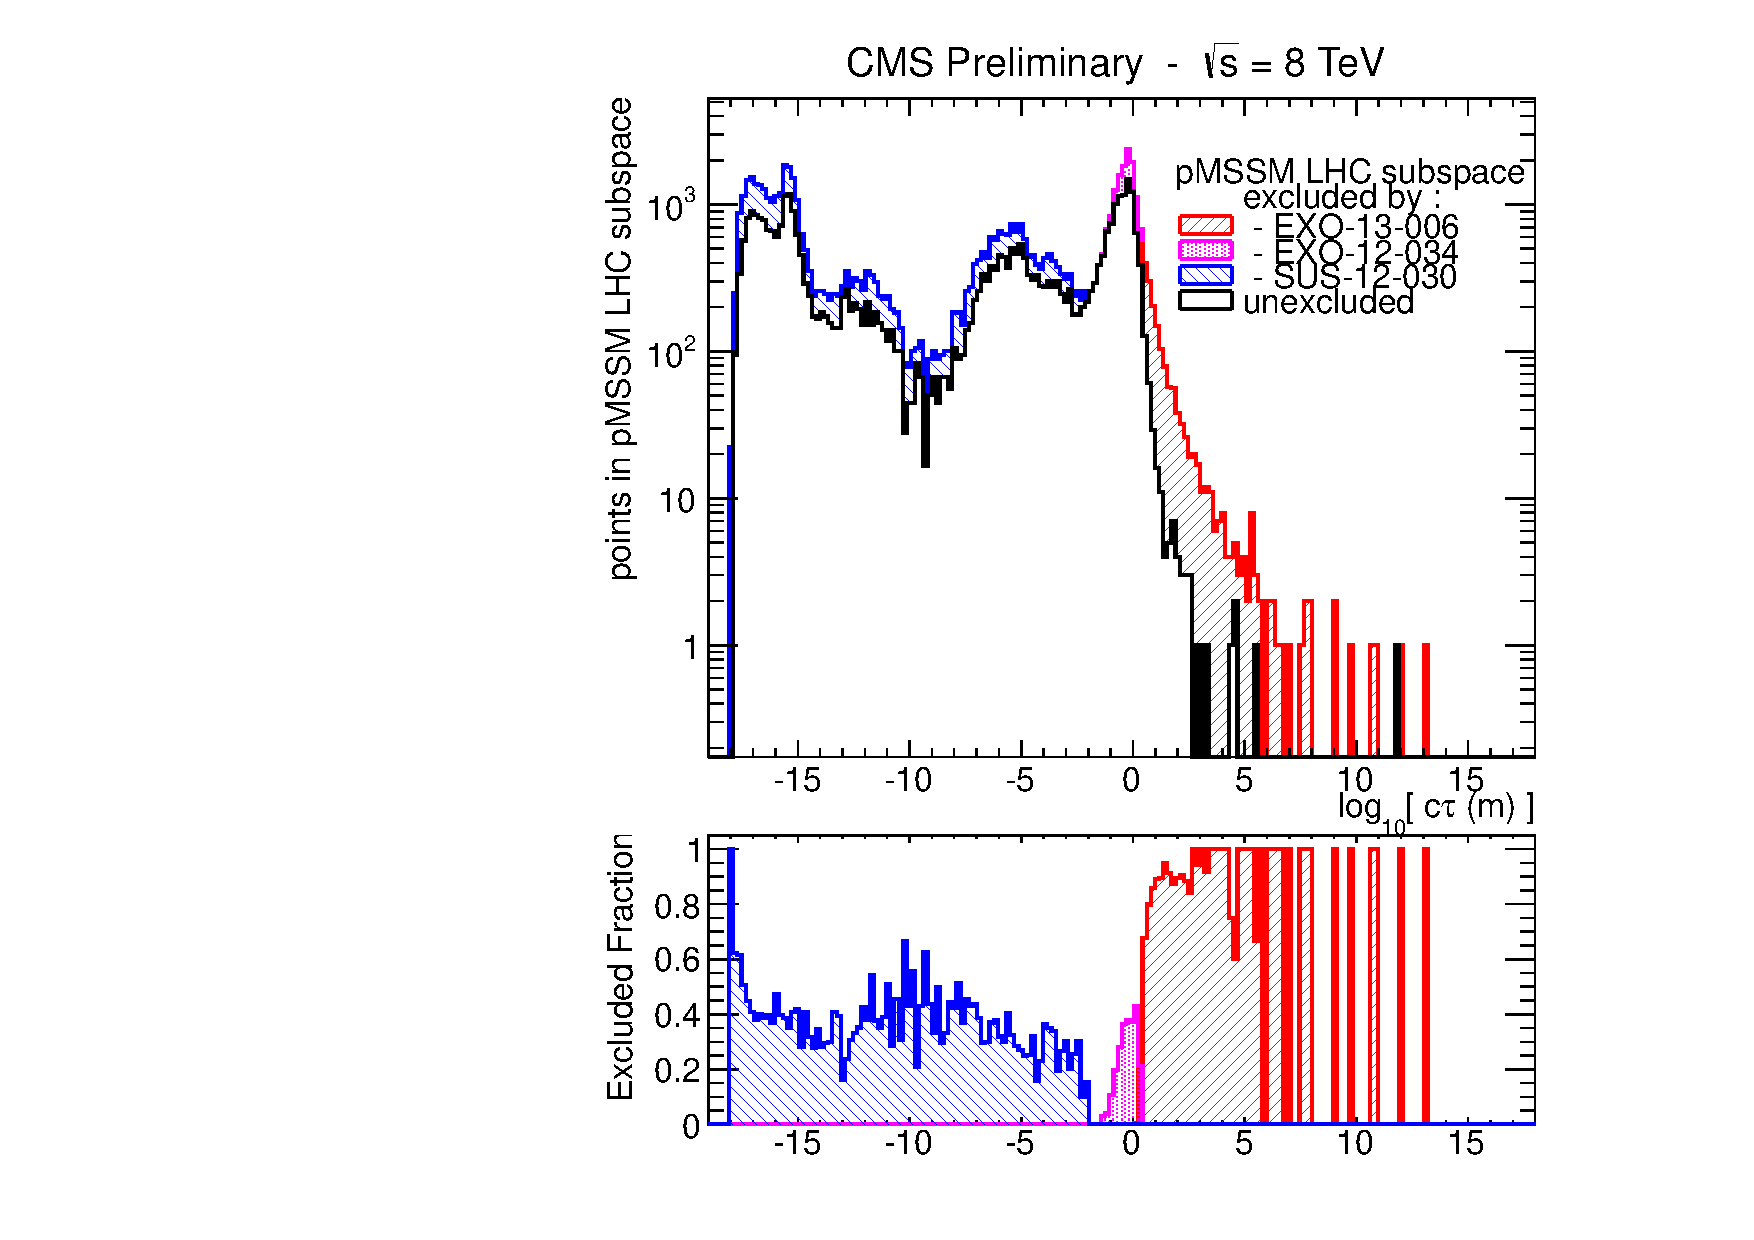
\includegraphics[width=0.75\textwidth]{figures/analysis/pMSSM_vs_ctau.pdf}
  \end{tabular}
  \caption{The number of excluded pMSSM points at 95\% C.L. (upper part) and the fraction of excluded pMSSM points (bottom part) vs. the chargino lifetime for different CMS searches.
           Red area: the search for long-lived charged particles \cite{bib:CMS:HSCP_8TeV},
           Purple area: the search for disappearing tracks  \cite{bib:CMS:DT_8TeV},
           Blue area: a collection of various general SUSY searches \cite{bib:CMS:pMSSMinterpretation_7TeV_PAS}
           The black line indicates the unexcluded pMSSM parameter points.
           The sampling of the parameter space points was done according to a prior probability density function which takes pre-LHC data and results from indirect SUSY searches into account (see \cite{bib:CMS:HSCPReinterpreation_PAS} for further details).
           Taken from: \cite{bib:pMSSMplot_source_from_DT}.}
  \label{fig:pMSSMplot}
\end{figure}
It can be seen that general SUSY searches (blue area) are sensitive to shorter chargino lifetimes ($c\tau \lesssim 10\cm$). 
Due to technical reasons\footnote{The pMSSM interpretation relied on the use of fast simulation techniques which are not capable of simulating charginos with lifetimes $\ctau>1\cm$.}, the general SUSY searches were never interpreted in the context of SUSY models with longer chargino lifetimes. 
Two existing searches, the search for long-lived charged particles~\cite{bib:CMS:HSCP_8TeV} and the search for disappearing tracks~\cite{bib:CMS:DT_8TeV} focus on long and intermediate chargino lifetimes, respectively. 
These two searches (purple and red areas) are sensitive to chargino lifetimes of $\ctau \gtrsim 35\cm$. 
Taken together, the existing searches exclude a large fraction of pMSSM points at different chargino lifetimes. 
However, there is a gap between the general SUSY searches and the search for disappearing tracks that is not accessible by any of the existing searches.\\

The here presented analysis aims at targeting this gap by optimising the search strategy for charginos with intermediate lifetimes of $10\cm \lesssim c\tau \lesssim 40\cm$. 
It is the first analysis at CMS focusing on two signature properties that are highly distinctive for charginos with intermediate lifetimes: first, the characteristically high ionisation losses of heavy charginos;
second, short reconstructed tracks due to chargino decays early in the detector. 

The associated challenges and the general search strategy of this analysis will be presented in the next section.

%%%%%%%%%%%%%%%%%%%%%%%%%%%%%%%%%%%%%%%%%%%%%%%%%%%%%%%%%%%%%%%%%%%%%%%%%%%%%%%%%%%%%%%%%%%%%%%%%%%%%%%%%%%%%%%%%%%%%%%%%%%%%%%%%%%%%%%%%%%%%%%%%%%%%%%%%%%%%%%%%%%%%%%%%%%%%%%%%%%%
%%%%%%%%%%%%%%%%%%%%%%%%%%%%%%%%%%%%%%%%%%%%%%%%%%%%%%%%%%%%%%%%%%%%%%%%%%%%%%%%%%%%%%%%%%%%%%%%%%%%%%%%%%%%%%%%%%%%%%%%%%%%%%%%%%%%%%%%%%%%%%%%%%%%%%%%%%%%%%%%%%%%%%%%%%%%%%%%%%%%
\FloatBarrier
\chapter{General search strategy}
\label{sec:GeneralSearchStrategy}

At the LHC, there are several possible chargino production channels. 
Chargino pairs can be produced through a photon or a $Z$-boson exchange. 
The chargino then decays via a virtual $W$-boson to the lightest neutralino and a fermion pair (\eg a pion). 
This process is illustrated in the Feynman diagram in Fig.~\ref{fig:FeynmanDiagram}.
Other possible chargino pair production channels include the exchange of a supersymmetric Higgs boson or a t-channel squark exchange (Fig.~\ref{fig:FeynmanDiagramProductionCharginoPair}).

Apart from pair production, charginos can be produced via the chargino neutralino production channel. 
On tree-level, there exist two production mechanisms: the s-channel $W$-boson exchange and the t-channel squark exchange (Fig.~\ref{fig:FeynmanDiagramProductionCharginoNeutralino}).

\begin{figure}[!t]
  \centering 
  \begin{tabular}{c}
    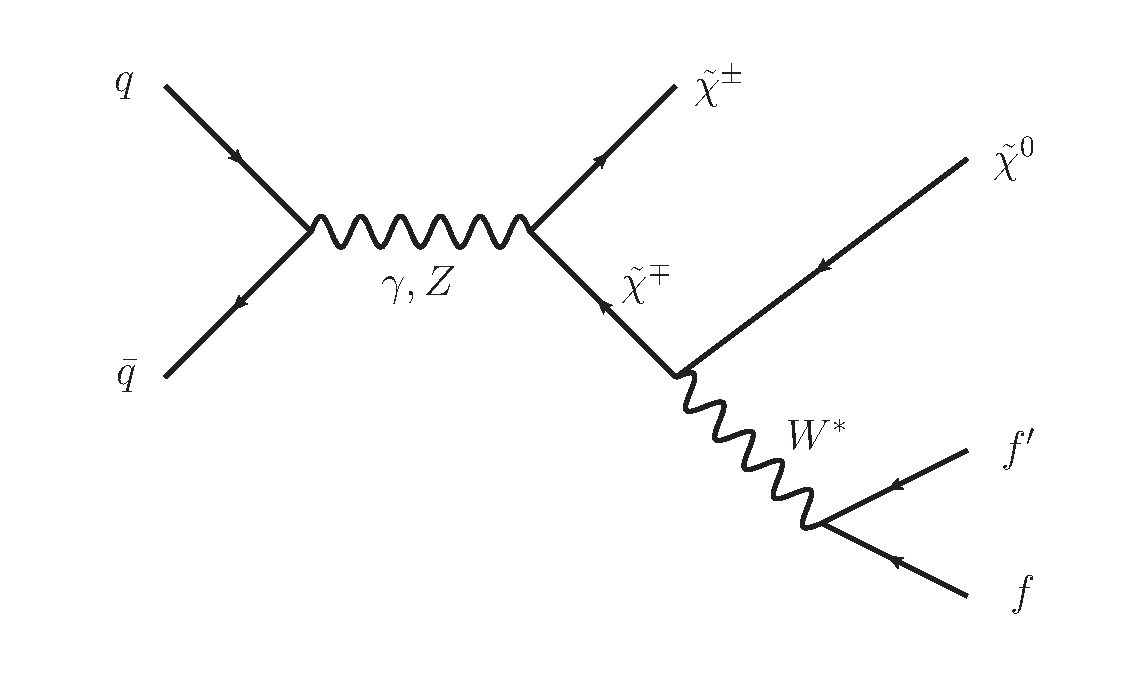
\includegraphics[width=0.75\textwidth]{figures/analysis/ChiChi_ProductionAndDecay.pdf}
  \end{tabular}
  \caption{Feynman diagram of chargino pair production via gamma or $Z$-boson exchange and the subsequent decay via a virtual $W$-boson.}
  \label{fig:FeynmanDiagram}
\vspace{25pt}
\end{figure}

\begin{figure}[!h]
  \centering 
  \begin{tabular}{c}
    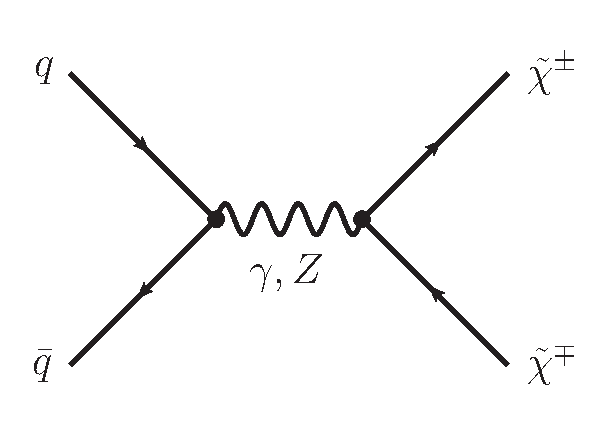
\includegraphics[width=0.33\textwidth]{figures/analysis/ChiChi_GammaZ.pdf}
    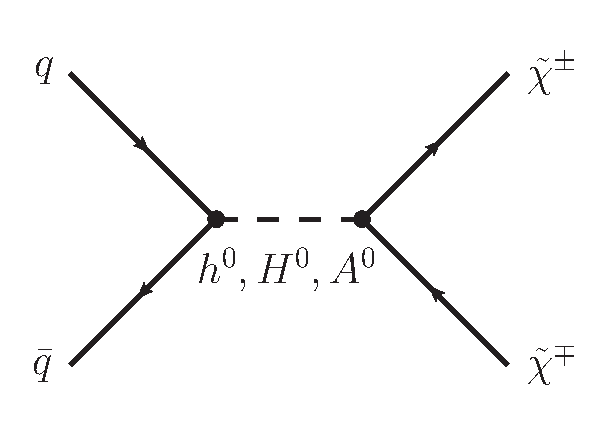
\includegraphics[width=0.33\textwidth]{figures/analysis/ChiChi_Scalar.pdf}
    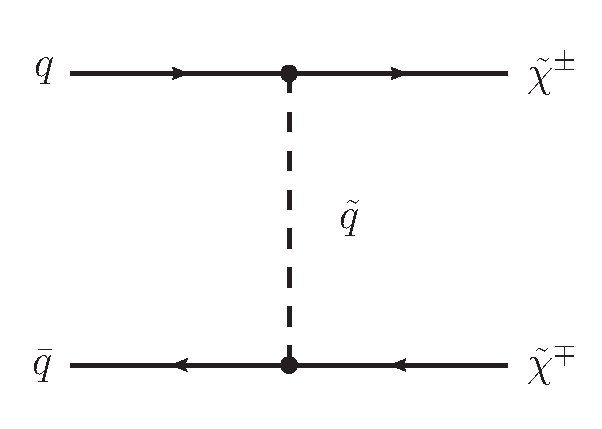
\includegraphics[width=0.33\textwidth]{figures/analysis/ChiChi_Squark.pdf}
  \end{tabular}
  \caption{Main tree-level diagrams for chargino pair production.}
  \label{fig:FeynmanDiagramProductionCharginoPair}
\vspace{25pt}
\end{figure}

\begin{figure}[!b]
  \centering 
  \begin{tabular}{c}
    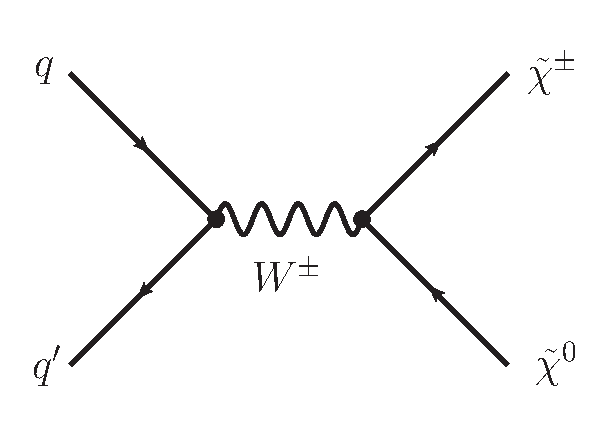
\includegraphics[width=0.33\textwidth]{figures/analysis/ChiChi0_WBoson.pdf}
    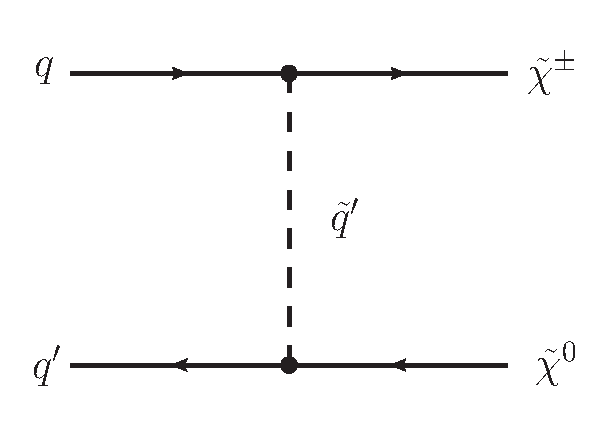
\includegraphics[width=0.33\textwidth]{figures/analysis/ChiChi0_Squark.pdf}
  \end{tabular}
  \caption{Main tree-level diagrams for chargino neutralino production.}
  \label{fig:FeynmanDiagramProductionCharginoNeutralino}
\end{figure}
Alternatively, charginos can be produced via strong production modes, \ie in cascade decays of new heavy particles, such as gluinos or squarks.
In those cascade decays, other particles are additionally produced and lead therefore to different signatures in the detector.
Thus, these strong production channels won't be considered in this analysis since they would require other optimised search strategies.\\
%Thus, the LHC offers the potential to search for charginos and due to its high centre-of-mass energy it is the first collider that can access SUSY models with charginos of several hundreds \gev.


When searching for supersymmetric models with long-lived \chipm, the strategy is of course highly dependent on the actual lifetime of the chargino. 
For long lifetimes, the chargino can reach the muon chambers and can be reconstructed as a muon even despite a longer time-of-flight \cite{bib:CMS:HSCP_7TeV}. 
For lower lifetimes, the chargino can already decay inside the detector (\eg the tracker), and can hence not be reconstructed as a muon but leads to an isolated, potentially disappearing track in the tracker. 
The detector signatures of these two scenarios are visualised in Fig.~\ref{fig:CharginoPaiEventDisplay}, where simulated chargino-chargino events are shown in a cross-sectional view of the CMS detector.
\begin{figure}[!b]
  \centering 
  \begin{tabular}{c}
  \begin{subfigure}{0.31\textwidth}
    \frame{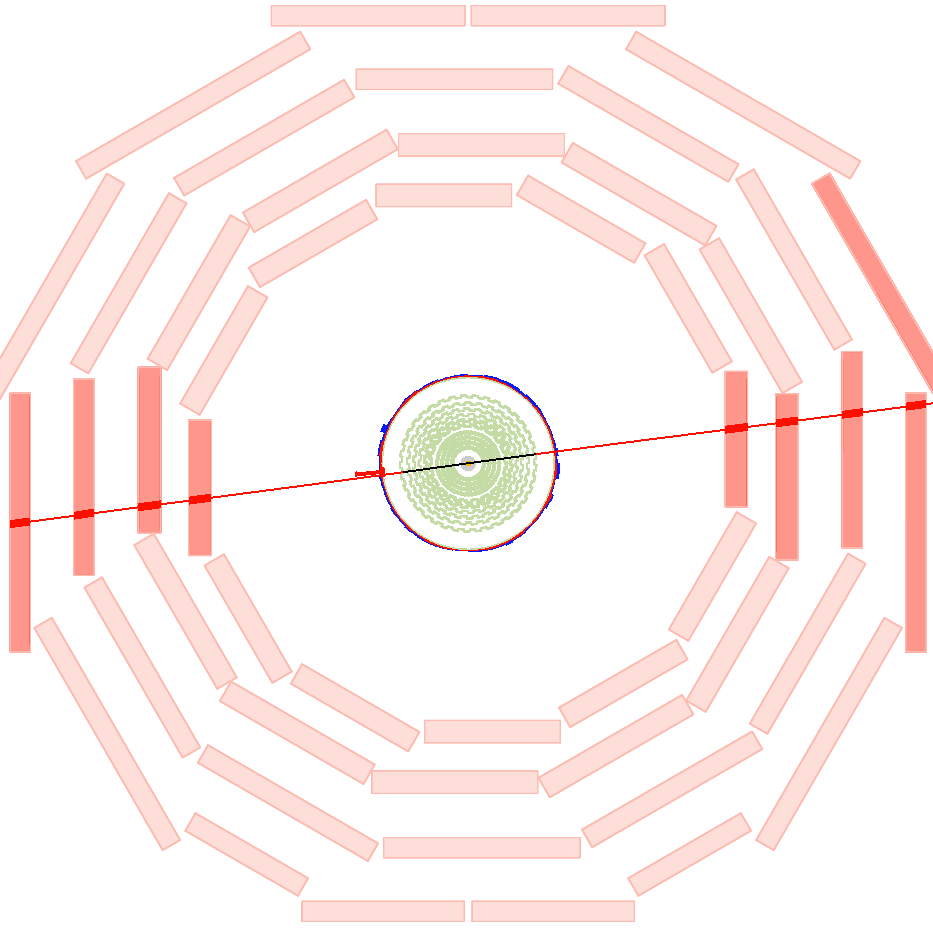
\includegraphics[width=0.99\textwidth]{figures/analysis/MotivationAndGeneralSearchStrategy/CharginoPairEvent_ctau_10000cm_lumi_1_event_12015.png}}
      \caption{}
  \end{subfigure} 
  \begin{subfigure}{0.31\textwidth}
    \frame{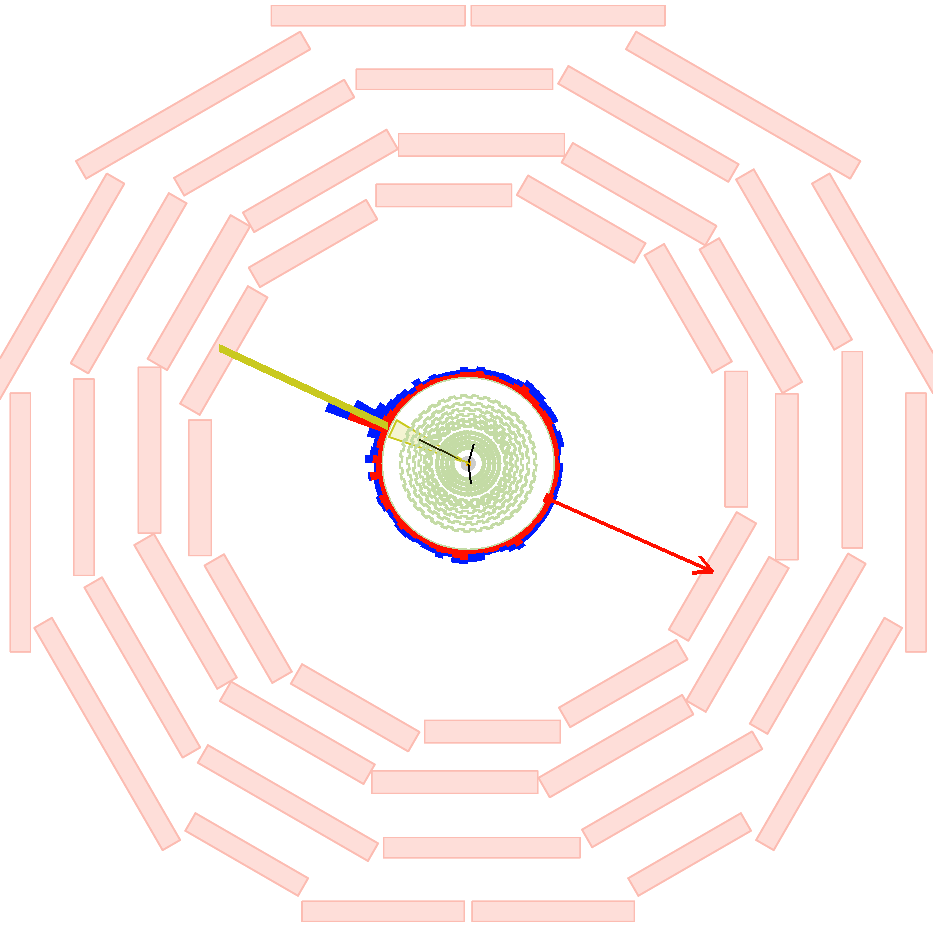
\includegraphics[width=0.99\textwidth]{figures/analysis/MotivationAndGeneralSearchStrategy/CharginoPairEvent_ctau_50cm_lumi_1_event_11024.png}}
      \caption{}
  \end{subfigure} 
  \begin{subfigure}{0.31\textwidth}
      \frame{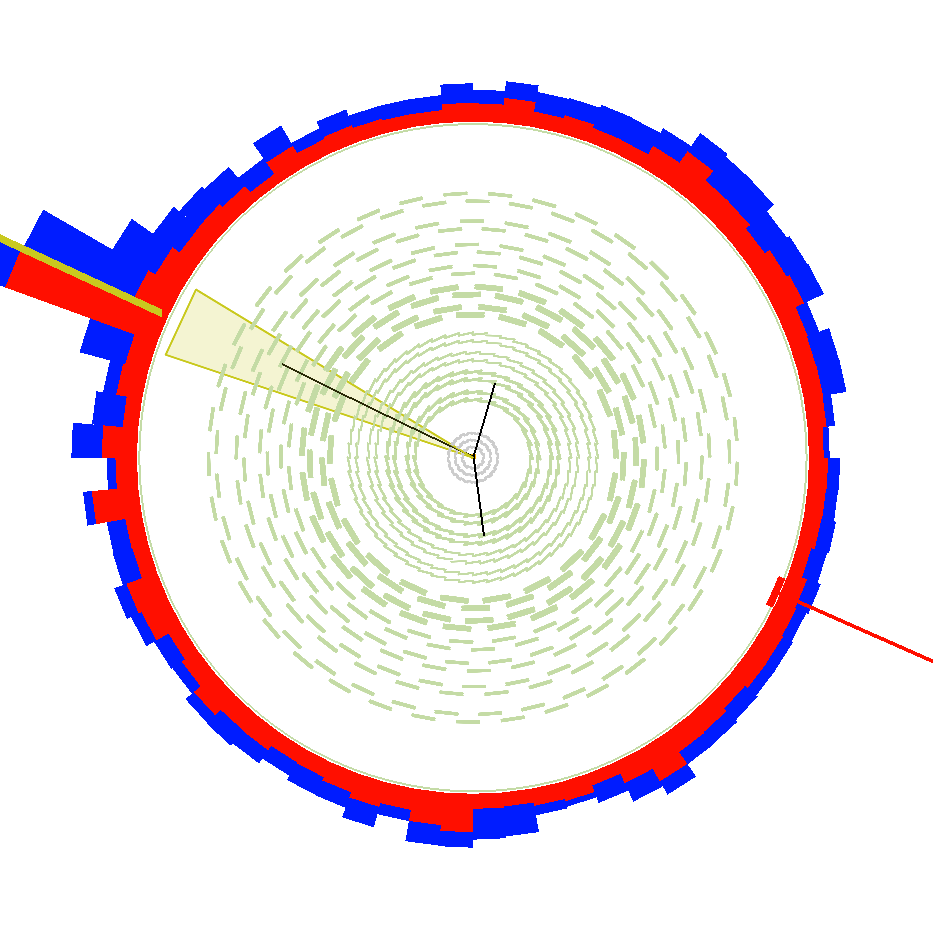
\includegraphics[width=0.99\textwidth]{figures/analysis/MotivationAndGeneralSearchStrategy/CharginoPairEvent_ctau_50cm_lumi_1_event_11024_Zoom.png}}
      \caption{}
  \end{subfigure} 
  \end{tabular}
  \caption{Visualisation of possible signatures of a chargino pair produced with a lifetime of $\ctau = 10\,\text{m}$ (a) and a lifetime of $\ctau = 0.5\,\text{m}$ (b and c). 
           The muon chambers are the outer layers of the detector and are depicted as red boxes.
           The black lines represent the reconstructed chargino tracks.
           The right picture is a zoom of the picture in the middle. Here, only the cross-section of the tracker (green wavy lines for the strip and grey lines for the pixel) is displayed. The red arrow shows the missing transverse energy in the event.
           The red (blue) towers correspond to the energy deposition in the ECAL (HCAL).} 
  \label{fig:CharginoPaiEventDisplay}
\end{figure}
In the left picture of Fig.~\ref{fig:CharginoPaiEventDisplay}, both charginos are reconstructed as muons, which can be seen in the energy deposition in the muon chambers.
In the middle and right pictures both charginos have a lower lifetime of $\ctau=0.5\,$m and thus are only visible as tracks in the tracker, where both trajectories end inside the silicon strip tracker.
Since this analysis targets a search for Supersymmetry with charginos of lifetimes between $\ctau \approx 10\,\text{cm} - 40\,\text{cm}$, the charginos decay rather early in the detector, even in the inner layers of the tracker.
%Thus, the signature of chargino events consists of isolated, short tracks that have large ionisation losses due to high chargino masses and the signatures of the decay products, \ie of a neutralino and a fermion pair. 
Thus, the signature of chargino events consists of isolated, short tracks and the signatures of the decay products, \ie of a neutralino and a fermion pair. 

In case of R-parity conservation one of the chargino decay products, the neutralino, is stable and weakly interacting, thus traversing the detector without leaving any further signature.
The missing transverse energy of the neutralino is balanced by the missing transverse energy of the second produced SUSY particle.
This is either a neutralino or the decay products of the chargino in events with chargino pairs. 

The signature of the other decay product, the fermion pair, can in principle be used to select chargino events. 
However, for mass-degenerate charginos, it can be very hard or even impossible to detect these fermions as will be explained in detail in the next paragraph.

First of all, the fermionic decay product (\eg a pion) can usually not be reconstructed because it does not origin from the primary vertex.
Secondly, it is very low in momentum because of the mass-degeneracy between \chipm and \chiO.
The typical momentum of a pion originating from a chargino to neutralino decay in the \chipm rest frame is of the order 
\begin{equation}
p_{\pi}\sim \sqrt{m_{\chi^{\pm}_1}-m_{\chi^{0}_1}-m_{\pi}}.
\end{equation}
%As the \chipm is rather slow for higher masses this is a good approximation also in the detector rest frame.
For a mass gap between \chipm and \chiO of $\Delta m=150\, \mev$, the pt distribution of the resulting pion peaks \mbox{at $\sim$ 100\,\mev} and ends at \mbox{\pt $\sim 400\,$\mev} (Fig.~\ref{fig:ptOfPions}).
\begin{figure}[!b]
  \centering 
  \begin{tabular}{c}
    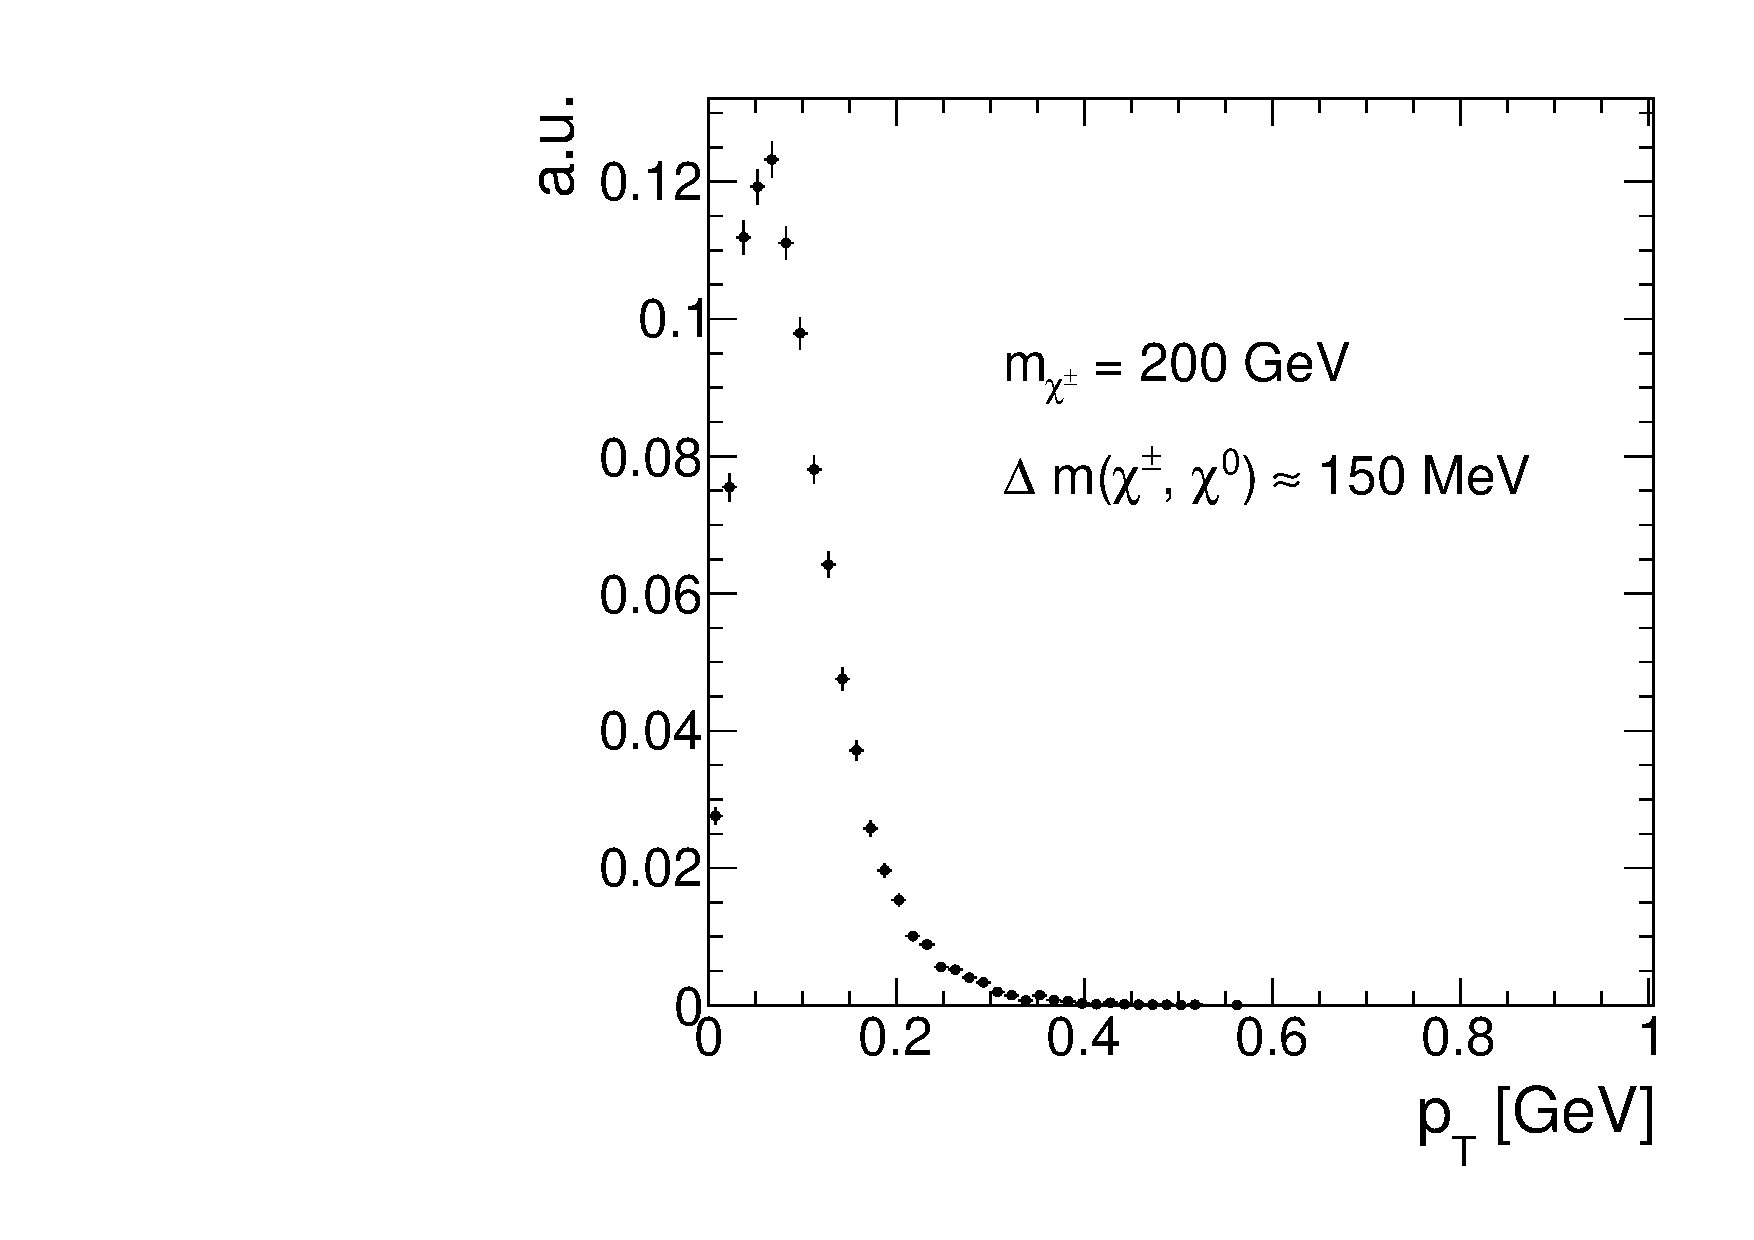
\includegraphics[width=0.49\textwidth]{figures/analysis/PtOfPions.pdf}
  \end{tabular}
  \caption{Transverse momentum distribution of pions coming from chargino decay into a neutralino with a mass gap of 150\mev.}
  \label{fig:ptOfPions}
%\vspace{90pt}
\end{figure} 

If the transverse momentum of a particle is very low, the particle trajectory is much more bended compared to a particle with higher \pt (see Fig.~\ref{fig:KinkedTrack} for illustration).
Due to this bending, the track reconstruction efficiency of particles with a transverse momentum below 1\gev decreases rapidly, reaching around 40\% for isolated pions with a \pt of 100\mev produced in the primary vertex~\cite{bib:CMS:tracking_8TeV}. 
It is therefore impossible to rely on a reconstruction of the fermionic chargino decay products in this analysis.
\begin{figure}[!b]
  \centering 
  \begin{tabular}{c}
    \frame{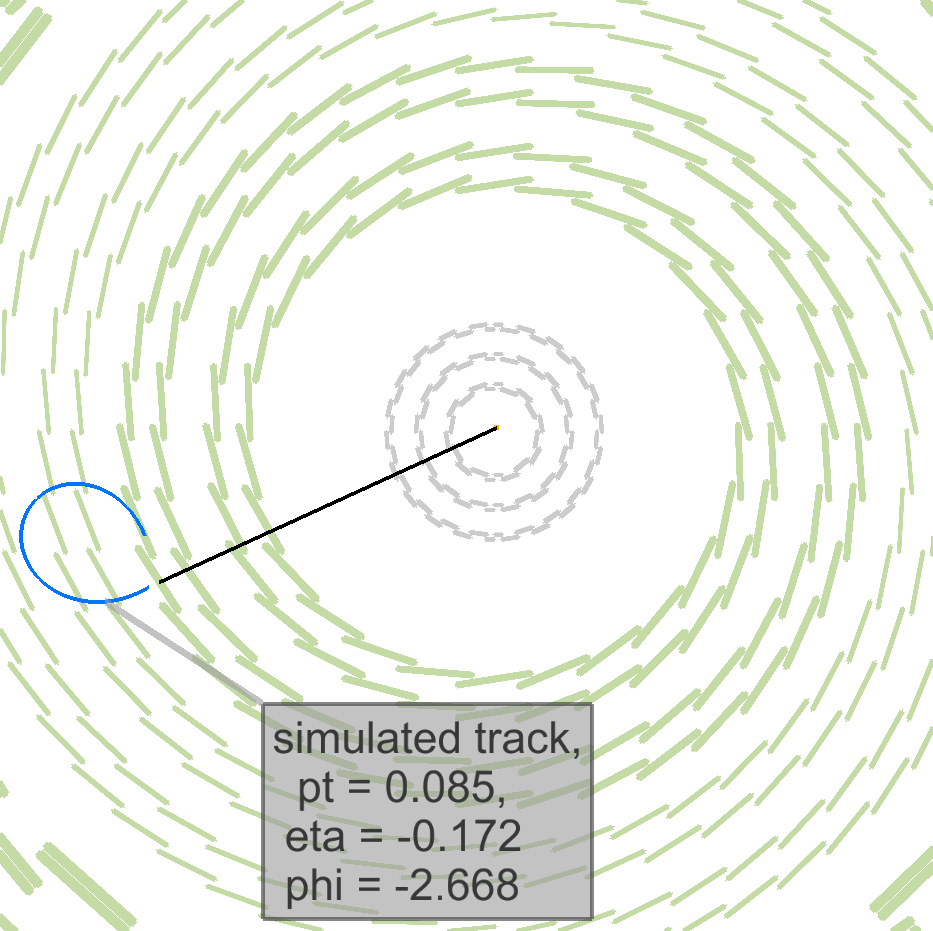
\includegraphics[width=0.4\textwidth]{figures/analysis/MotivationAndGeneralSearchStrategy/BendedPionTrack.png}}
    %\frame{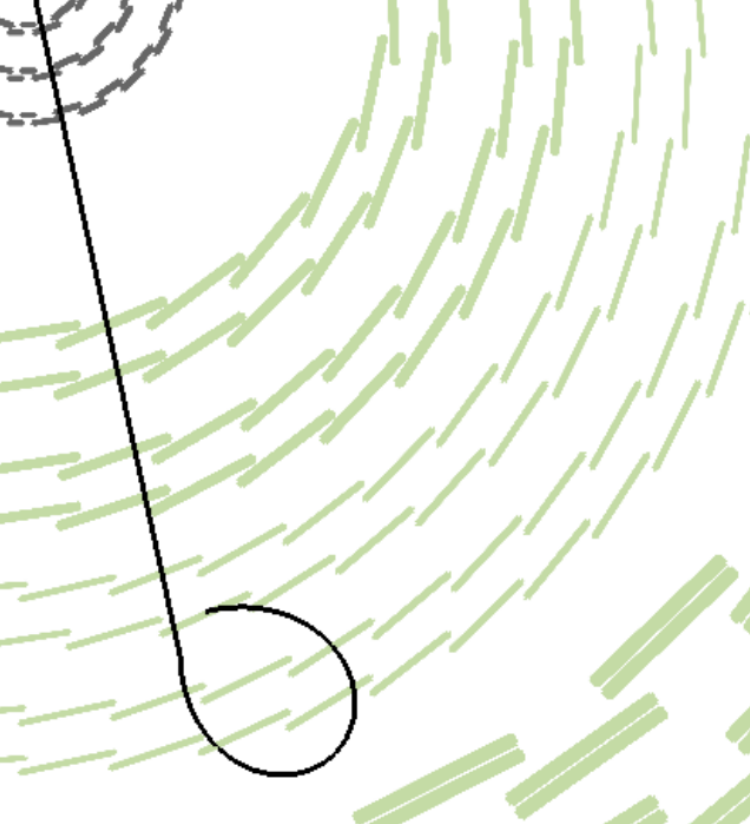
\includegraphics[width=0.30\textwidth]{figures/analysis/KinkedTrackZoom_Quadrat.png}}
  \end{tabular}
  \caption{Cross-sectional view of the tracker (silicon strip (silicon pixel) tracker layers are illustrated with green (grey) lines) and a simulated chargino track (black line) decaying to a pion (bended blue line) with a \pt of $\sim$85\mev and a neutralino (not visible).}
  \label{fig:KinkedTrack}
\end{figure} 


In summary, the signature of chargino events in mass-degenerate SUSY models consists only of a - potentially - disappearing track. 
Such a signature is very difficult to detect, especially since CMS doesn't offer a dedicated track trigger so that triggering on the chargino track is impossible.

In order to search for such signatures, one therefore needs to trigger on other, less obvious properties of chargino events. 
This analysis takes advantage of higher order contributions to the Feynman diagrams shown in Figs.~\ref{fig:FeynmanDiagramProductionCharginoPair} and~\ref{fig:FeynmanDiagramProductionCharginoNeutralino}, resulting in initial state radiation (ISR).
If the initial quarks radiate a high \pt gluon, the resulting jet can be detected and can offer a possibility to search for events with nothing more than isolated tracks.
Furthermore, the non-detection of the chargino's decay products plus a high \pt ISR jet lead to missing transverse energy (MET) in the event. 
Exploiting these two circumstances, it is possible to detect chargino-pair or chargino-neutralino events with the help of Jet+MET triggers.

Since Jet+MET triggers are not very specific for chargino events, it is important to identify further track properties that can be used to select chargino candidates.
One distinctive property of charginos compared to SM particles is their high mass. 
Therefore, charginos can be identified by selecting high \pt tracks. 
Furthermore, the energy loss per path length (\dedx) depends quadratically on the particle's mass for low velocities ($0.2<\beta\gamma<0.9$):
\begin{equation*}
\langle\frac{dE}{dx}\rangle = K \frac{m^2}{p^2} +C
\end{equation*}
Therefore, \dedx constitutes a very nice discriminating variable for massive particles like charginos against SM particles.
The selection of chargino events in this analysis thus relies on the selection of isolated high \pt tracks with high \dedx values. 

If the chargino decays before it has crossed the full pixel and strip detector, the associated track is disappearing. 
For low lifetimes, the tracks can be very short and can have only a few hits in the detector. 
In order to reconstruct a particle's trajectory, a minimum of three hits are required since defining a helical path requires five parameters (see \cite{bib:CMS:tracking_8TeV}). 
A specific challenge for this analysis is hence the combination of searching for short tracks and utilising the measurement of the energy deposition of the chargino. 
For very short tracks, eventually only passing the first couple of layers of the whole tracker system, the pixel tracker information becomes very important. 
Therefore, an accurate energy measurement in the pixel system is of great importance to this analysis. 
However, no other CMS analysis has used the energy information of the pixel tracker so far.
This analysis thus requires a thorough study of the quality of the pixel energy calibration and, potentially, a recalibration in case the pixel energy calibration is not sufficient.



\section{Comparison to earlier searches}
As already mentioned before, there are two analyses at CMS at $\sqrt{s}=8\,\tev$ with 20\,fb$^{-1}$ data that search for intermediate lifetime charginos, the search for long-lived charged \mbox{particles \cite{bib:CMS:HSCP_8TeV}} and the search for disappearing tracks \cite{bib:CMS:DT_8TeV}.
The here presented analysis aims at achieving an increase in sensitivity towards shorter lifetimes compared to the earlier analyses in a twofold way.
First, the selection is optimised for the inclusion of very short tracks.
Second, the inclusion of the variable \dedx is used to increase the search sensitivity compared to \cite{bib:CMS:DT_8TeV}.\\

In \cite{bib:CMS:HSCP_8TeV}, a minimum number of eight hits were required for every track, whereas \cite{bib:CMS:DT_8TeV} required a minimum of seven hits.
This can be very inefficient for shorter lifetimes, where most of the charginos already decay shortly after the pixel tracker.
In Fig.~\ref{fig:NHits_2Signal_noSelection_normalized} (left), the normalised distribution of the number of measurements (\nhits) of chargino tracks is shown. 
It can be seen, that \nhits peaks at the minimal possible value needed for track reconstruction of $\nhits=3$ for lower lifetimes.
%For higher lifetimes ($\ctau=50\cm$) the distribution shifts to higher values with a second peak at $\nhits\sim17$.
For a lifetime of $\ctau=50\cm$, a second peak at $\sim$17 hits appears corresponding to the number of measurements when crossing all pixel barrel (3) and strip inner and outer barrel (6 from stereo and 8 from normal) layers.
However, a notable fraction of $\sim$ 40\% of chargino tracks still has a number of measurements of $\nhits<8$. 

It should be also mentioned, that the track reconstruction efficiency is sufficient for short chargino tracks, such that a loosening of the \nhits requirement is expected to be really improving the signal acceptance.
The track reconstruction efficiency for different chargino decay points is depicted in Fig.~\ref{fig:NHits_2Signal_noSelection_normalized} (right).
For very short tracks ($\nhits=3$) the efficiency is still around 20\%.\\
\begin{figure}[!t]
  \centering 
  \begin{tabular}{c}
  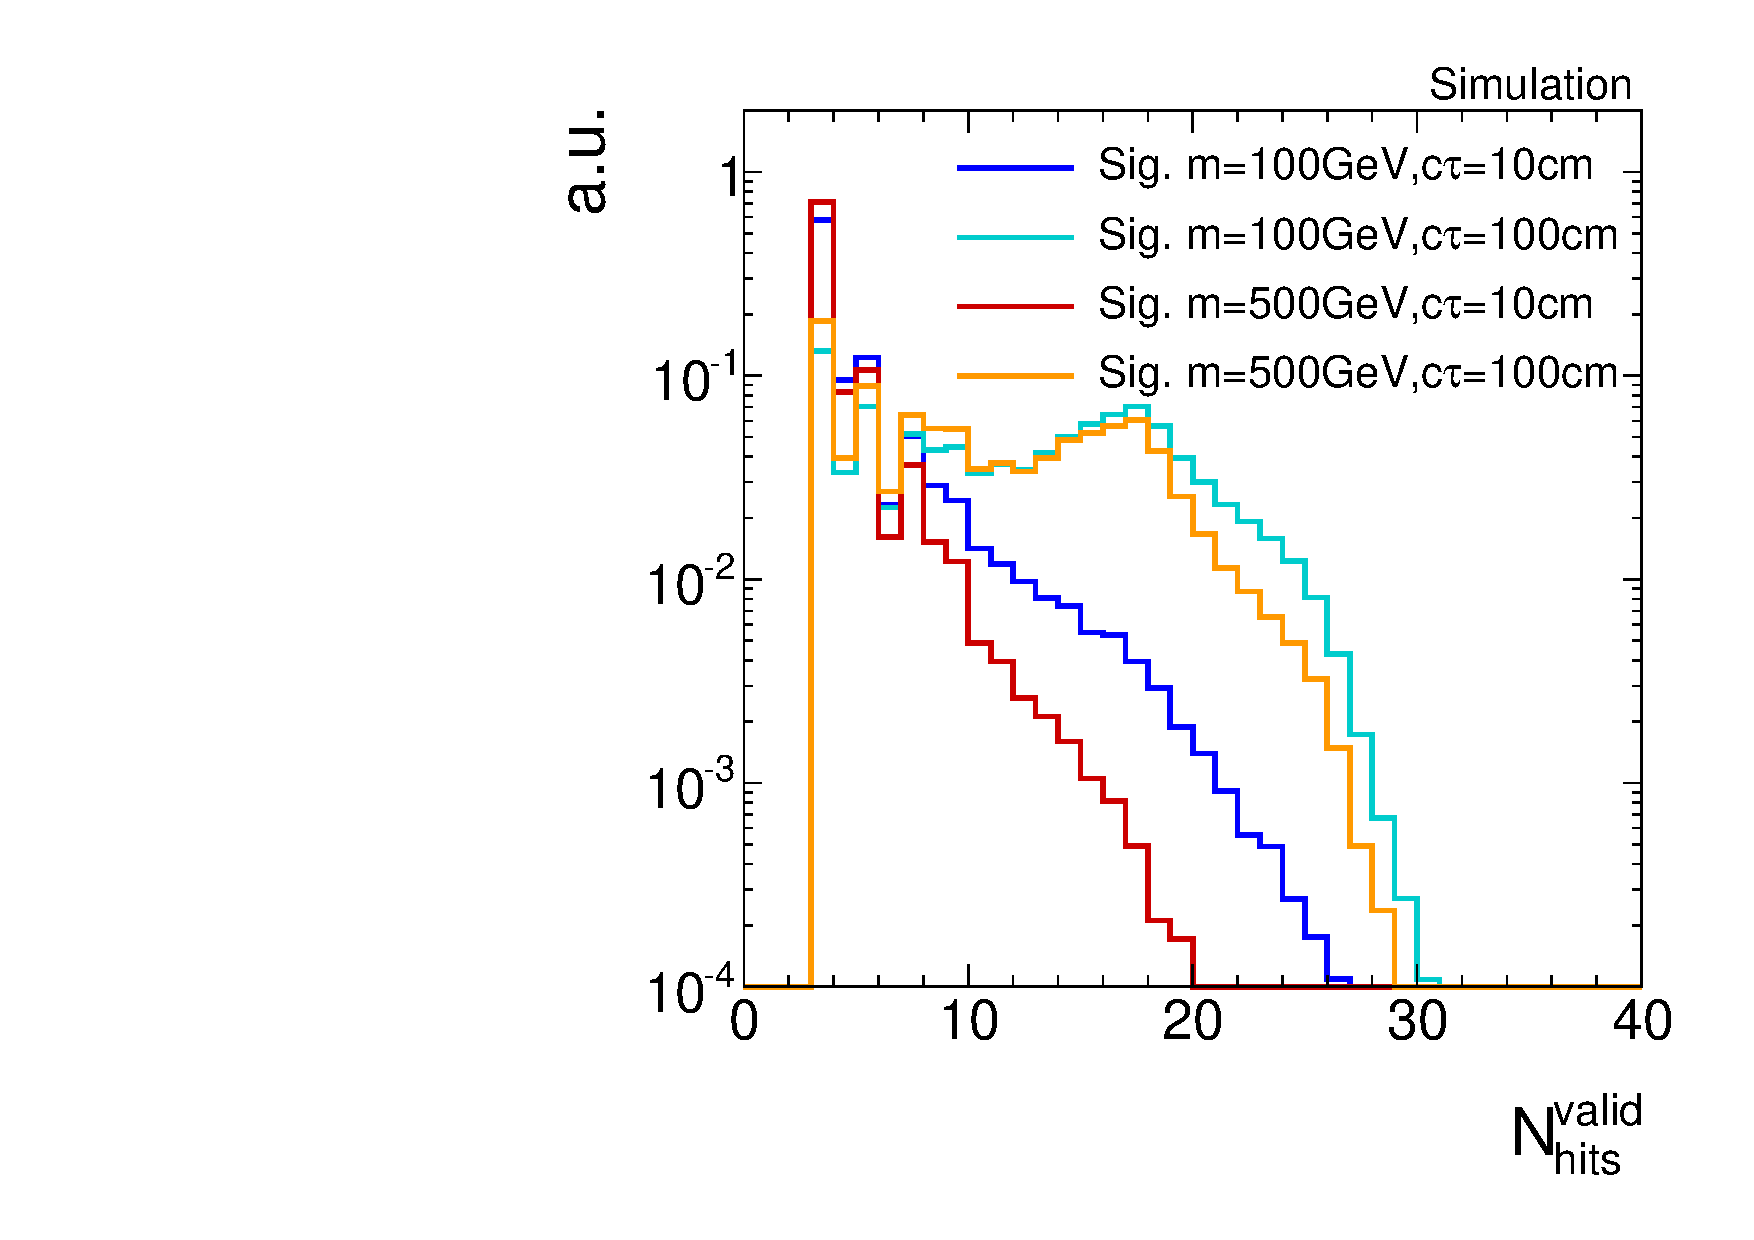
\includegraphics[width=0.49\textwidth]{figures/analysis/MotivationAndGeneralSearchStrategy/htrackNValid_log_chiTracksnoSelection.pdf}
  %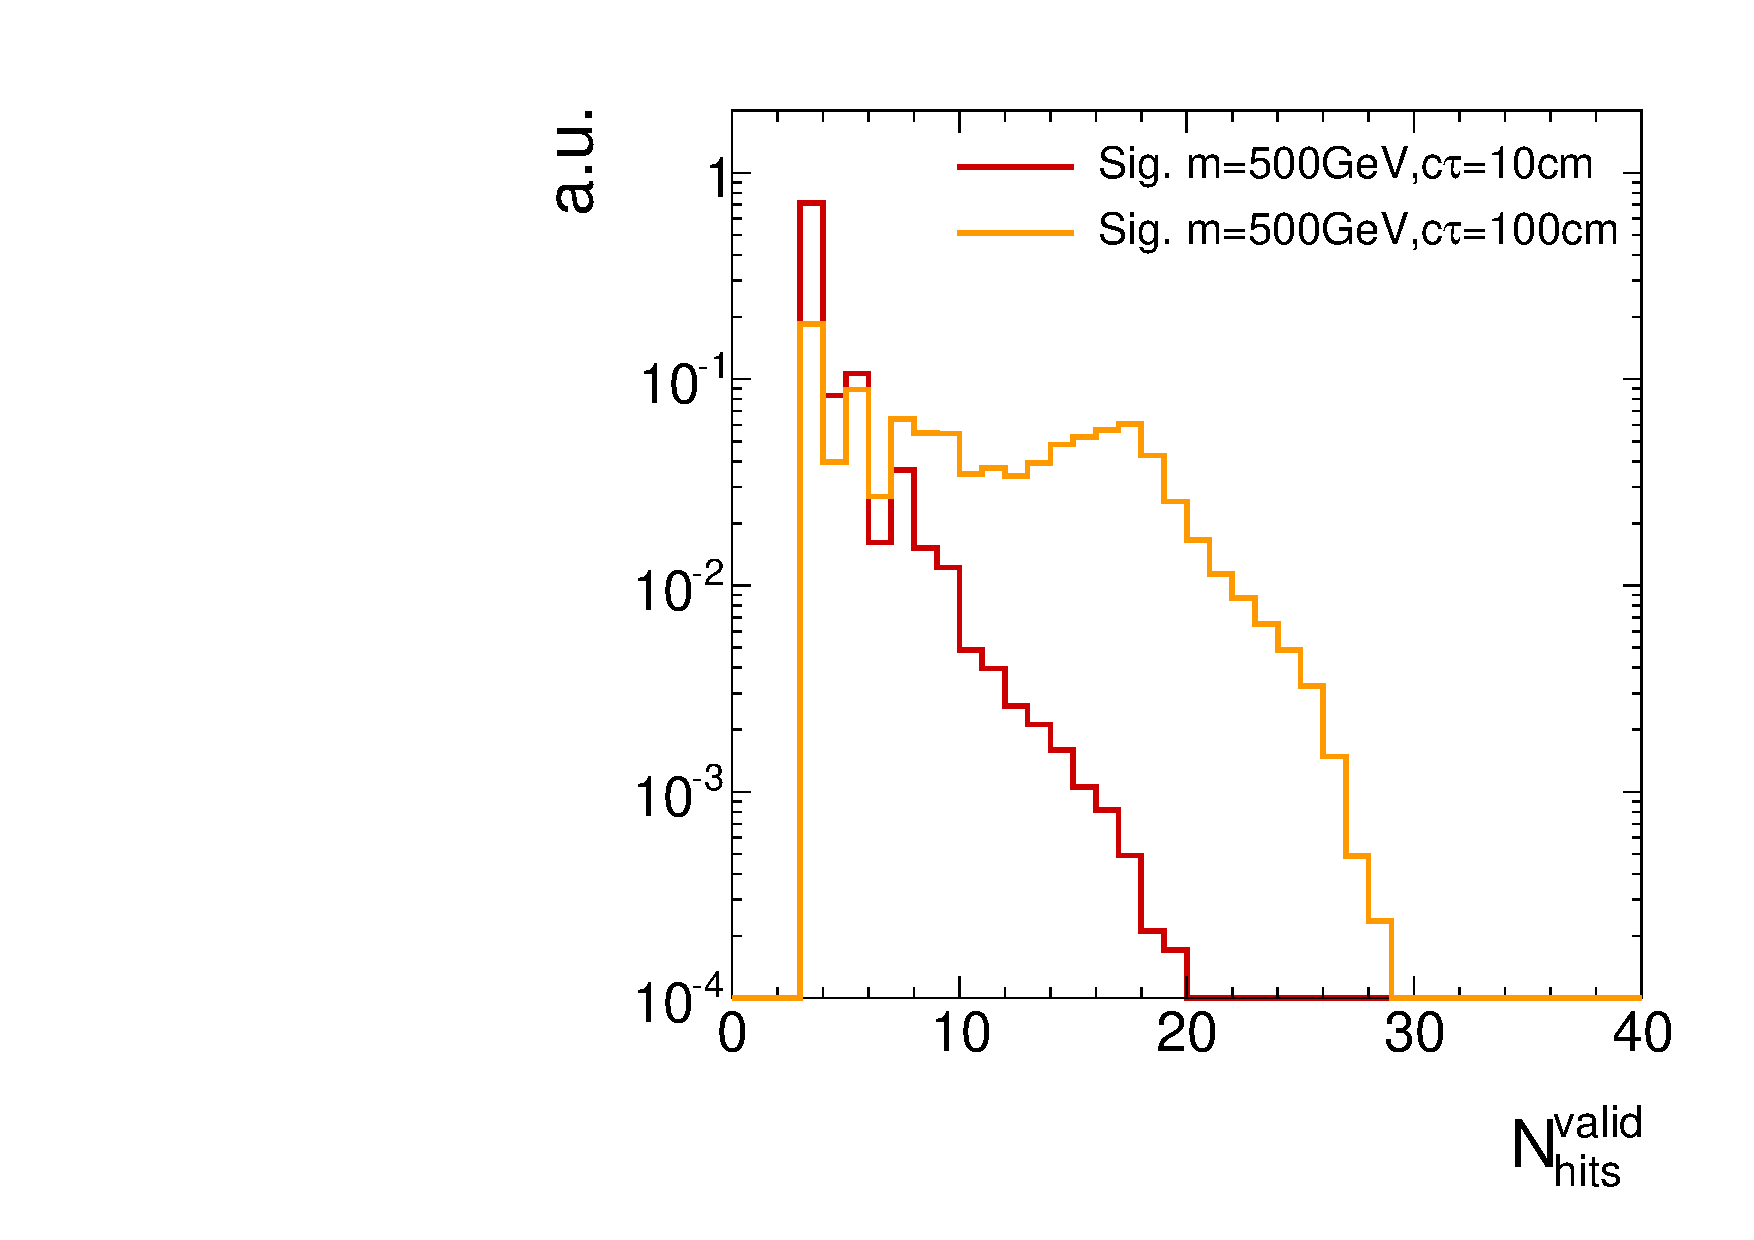
\includegraphics[width=0.49\textwidth]{figures/analysis/htrackNValid_log_chiTracksnoSelection_m500GeV.pdf}
  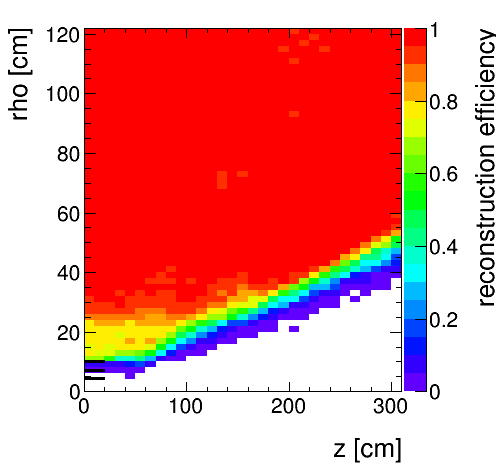
\includegraphics[width=0.49\textwidth]{figures/analysis/MotivationAndGeneralSearchStrategy/RecoEffTracksZoom.png}
  \end{tabular}
  \caption{Left: Number of measurements in the tracker system \nhits for four different signal lifetimes.
           Right: Probability to reconstruct a track (z) in dependency of the chargino's decay point (x and y).
           More information on the generation of the simulated signal samples can be found in Section~\ref{sec:SignalSamples}.} 
  \label{fig:NHits_2Signal_noSelection_normalized}
\end{figure}



Additionally, the search for disappearing tracks which targets models with charginos decaying inside the tracker did not make use of the high energy deposition of heavy particles. 
Although this variable was indeed used in the search for long-lived charged particles, this search was not optimised for intermediate lifetimes (\eg no explicit muon veto on the selected tracks was required). 
Thus, it shows less sensitivity compared to the disappearing track search in the lifetime region between $35\,\text{cm} \lesssim c\tau \lesssim 100\,\text{cm}$ (see Fig.~\ref{fig:pMSSMplot}).\\

To conclude, the general search strategy of the here presented analysis is to unite the strategies of \cite{bib:CMS:HSCP_8TeV} and \cite{bib:CMS:DT_8TeV} and to lower the strong selection on the number of hits in these analyses in order to get an optimised selection for lifetimes around $10\,\text{cm} \lesssim c\tau \lesssim  40\,\text{cm}$.

%%%%%%%%%%%%%%%%%%%%%%%%%%%%%%%%%%%%%%%%%%%%%%%%%%%%%%%%%%%%%%%%%%%%%%%%%%%%%%%%%%%%%%%%%%%%%%%%%%%%%%%%%%%%%%%%%%%%%%%%%%%%%%%%%%%%%%%%%%%%%%%%%%%%%%%%%%%%%%%%%%%%%%%%%%%%%%%%%%%%
%%%%%%%%%%%%%%%%%%%%%%%%%%%%%%%%%%%%%%%%%%%%%%%%%%%%%%%%%%%%%%%%%%%%%%%%%%%%%%%%%%%%%%%%%%%%%%%%%%%%%%%%%%%%%%%%%%%%%%%%%%%%%%%%%%%%%%%%%%%%%%%%%%%%%%%%%%%%%%%%%%%%%%%%%%%%%%%%%%%%
\FloatBarrier
\chapter{Improved dE/dx measurement for short tracks}
\label{sec:DeDxMeasurement}
As already pointed out in the previous chapter the inclusion of the pixel energy measurements can increase the sensitivity when searching for short and highly ionising tracks.
While the silicon strip detector has already been calibrated as part of the search for long-lived charged particles \cite{bib:CMS:HSCP_8TeV}, no complete calibration has been done for the pixel silicon tracker so far.
To increase the discrimination power of \dedx for short tracks, such a calibration procedure is therefore conducted within this PHD thesis.

The CMS tracker system provides a measurement of the particle's energy loss for each hit in the tracker.
This is done by the detection of the number of electrons produced by the ionisation of the silicon.
A detailed introduction to the CMS tracker system and the energy measurement can be found in Section~\ref{FIXME}.

How to combine the single energy measurements for each tracker hit into one track \dedx estimator that can be used for analysis porpuses will be explained in the following Section~\ref{sec:sub:MeasuringDeDx}.
The pixel energy calibration is then described in Section~\ref{sec:EnergyCalibration}. 
How to discrimate SM particles and beyond SM particles with the help of a \dedx measurement is discussed in Section~\ref{sec:Ias}, followed by the exploration of the achieved discrimination improvements in Section~\ref{sec:DiscriminationImprovements}.

%The CMS tracker system does not only allow for the precise measurement of particle tracks and primary and secondary vertices but also the measurement of a particle's mean energy loss per path length.
%This is done by the detection of the number of electrons produced by the ionisation of the particle during its passage through the silicon tracker.
%A detailed introduction to the CMS tracker system and the energy measurement can be found in Section~\ref{FIXME}.

%It was already pointed out that the inclusion of the pixel energy measurements can increase the sensitivity when searching for short and highly ionising tracks.
%While the silicon strip detector has already been calibrated as part of the search for long-lived charged particles \cite{bib:CMS:HSCP_8TeV}, no complete calibration has been done for the pixel silicon tracker so far.
%To increase the discrimination power of \dedx for short tracks, such a calibration procedure is therefore conducted within this PHD thesis.


\section{Ionisation loss of charged particles}
\label{sec:sub:MeasuringDeDx}
Energy losses for moderately relativistic charged particles travelling through matter are mostly caused by ionisation effects.
The mean energy loss per path length can be described with the Bethe formula \cite{bib:Bethe_1930}:
\begin{equation}
\langle \frac{dE}{dx} \rangle = Kz^2\frac{Z}{A}\frac{1}{\beta^2} [ \frac{1}{2} \ln{\frac{2m_e c^2 \beta^2 \gamma^2 T_{\text{max}}}{I^2}} - \beta^2 - \frac{\delta( \beta \gamma )}{2} ].
\end{equation}
It is a function of the atomic number ($Z$), the atomic mass ($A$) of the absorber, and the mean excitation energy ($I$) which is 173\,eV for silicon~\cite{bib:NIST}.  
$T_{\text{max}}$ represents the maximum energy transfer in a single collision.
The relevant particle's properties are the velocity ($\beta$), the Lorentz factor ($\gamma$) and the charge (z) of the incident particle.
The density correction $\delta( \beta \gamma )$ reduces the mean energy loss at high energies because of polarisation effects of the material. 
%The constant factor K is $4\pi N_A r_e^2 m_e^2 c^2$ with $N_A$ being the Avogadro constant, $m_e$ the electron mass and $r_e$ the classical electron radius of 2.8\,fm.
The factor K is constant and is 0.307 in units of $\mev\,$mol$^{-1}$cm$^2$.
The Bethe formula is valid if the main energy loss originates from ionisation effects, \ie in a region between $0.1\lesssim\beta\gamma\lesssim 1000$.


Even if widely used, the mean energy loss is a quantity which is ``ill-defined experimentally and is not useful for describing energy loss by single particles'' \cite{bib:PDG_2014}.
The problem is caused by the underlying probability distribution of one single \dedx measurement (this will be named $\Delta E/ \Delta x $ throughout the following sections), which can be parametrised by a Landau distribution \cite{bib:Landau_1944}
\begin{equation}
p(x) = \frac{1}{\pi} \int_0^\infty\! e^{-t \log t - x t} \sin(\pi t)\, dt.
\end{equation}
The Landau distribution has no free parameters. Its most probable value is around 0.222.
However, it is possible to introduce artificially a different most probable value and a width (at half maximum) with $x \rightarrow \frac{x-\text{MPV}}{\sigma}-0.222$.
The Landau distribution is a highly asymmetric distribution with a long tail towards the right end (see Fig.~\ref{fig:landau}).
\begin{figure}[!t]
  \centering 
  \begin{tabular}{c}
  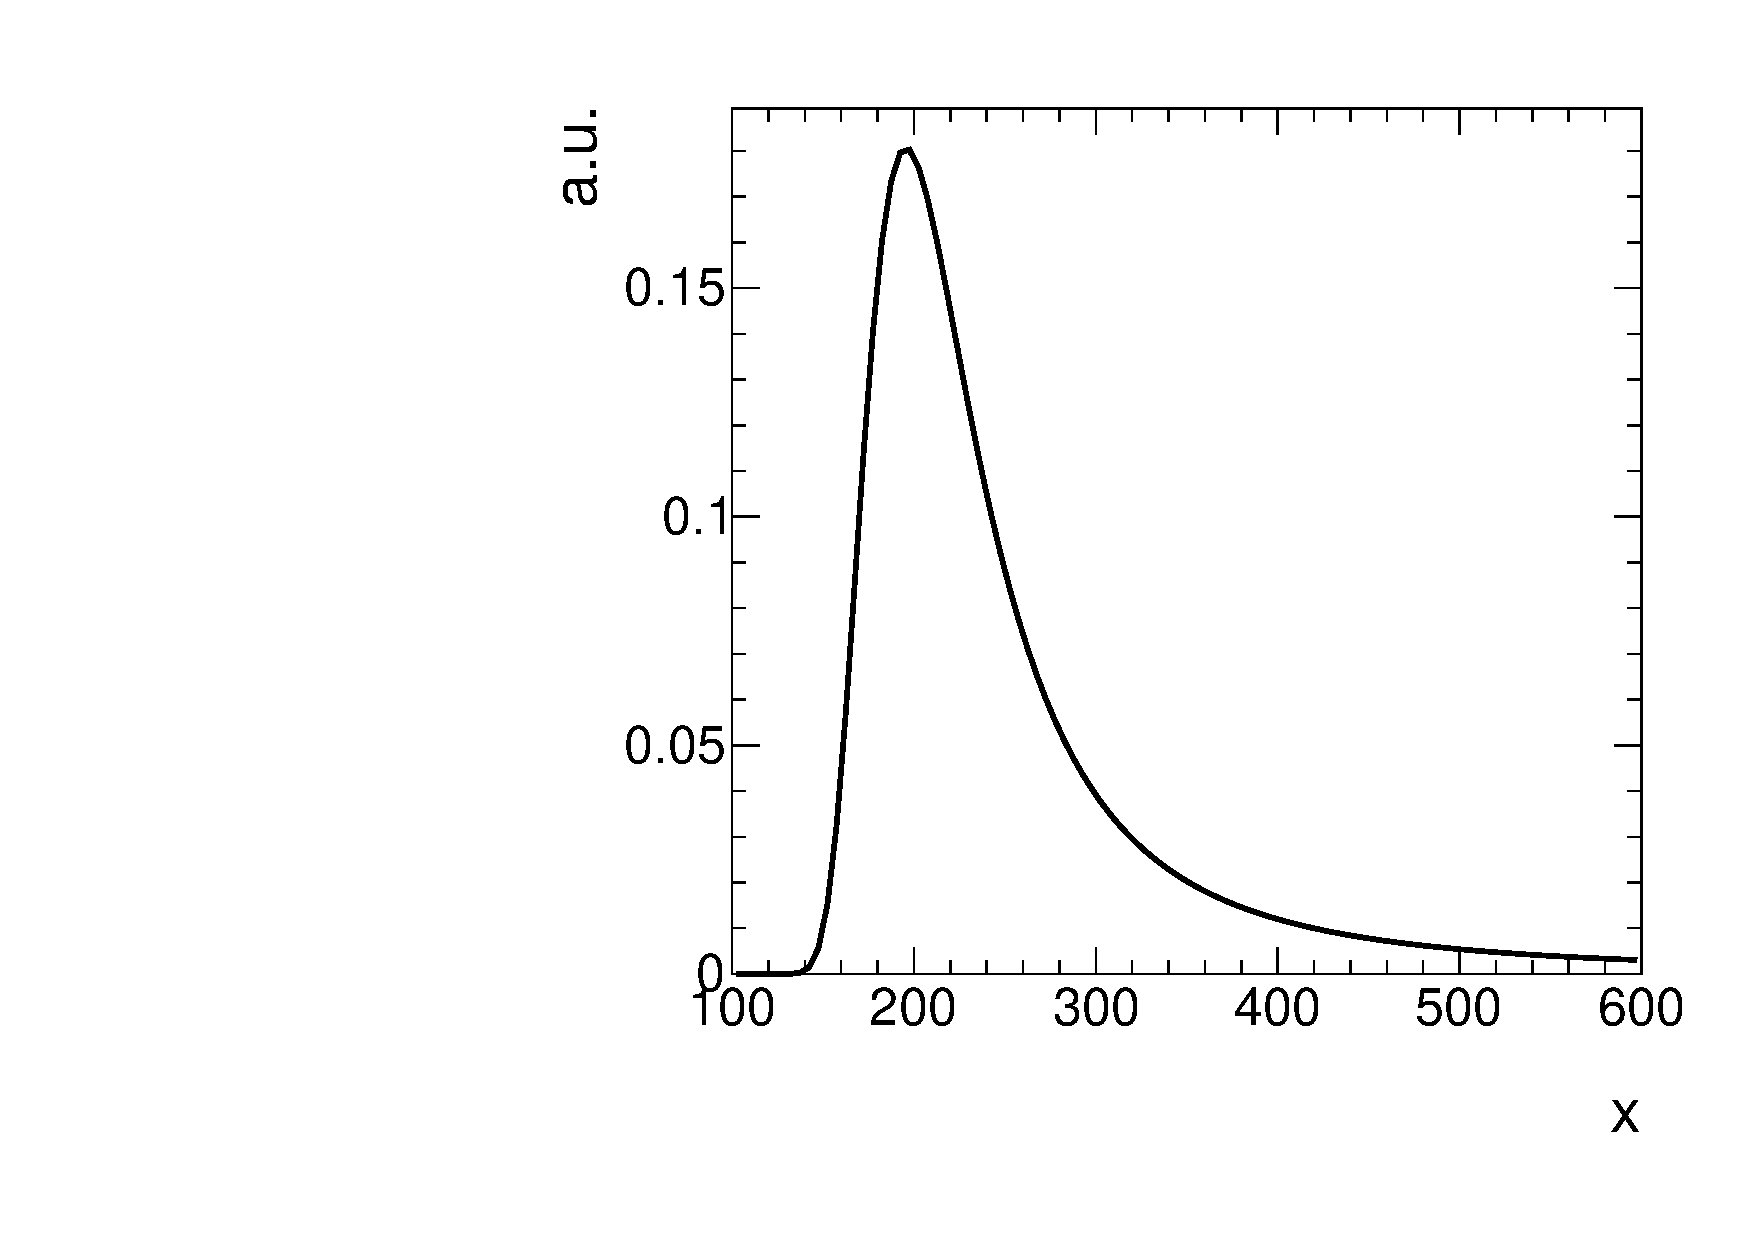
\includegraphics[width=0.49\textwidth]{figures/analysis/PixelCalibration/Landau.pdf}
  \end{tabular}
  \caption{Illustration of the shape of a Landau distribution. Parameters were chosen as $\mu=200$ and $\sigma=20$.} 
  \label{fig:landau}
\end{figure}
Theoretically it extends to infinite energies, however in nature the maximal deposited energy is of course limited by the particle's full energy.
%The mean and the variance of a landau distribution are not defined.
Because of its strong asymmetry, measurements of the mean energy loss per path length $\langle \dedx \rangle$ with only a few single measurements are easily fluctuating towards high values.
This makes the use of the mean energy loss described by the Bethe formula for the discrimination of new heavy particles problematic, because massive particles realease in general higher amounts of energy in matter.
%This is again different for a (limited) measurment, as there it is always possible to calucalute a mean.
%Still, this leads to the fact that the definition of the mean energy loss per path length is a problematic and unstable concept.


A much better observable is the most probable value (MPV) of the Landau distribution.
The MPV is much more stable compared to the mean and is not as easily fluctuating to higher \dedx values. 
The most probable energy loss of a charged particle, $\Delta_p$, can be described by the Landau-Vavilov-Bichsel equation \cite{bib:Bichsel:MPV_1988}:
\begin{equation}
\Delta_p = \xi \left[ \ln \frac{2m_e c^2\beta^2\gamma^2}{I}  + \ln\frac{\xi}{I} + j - \beta^2 - \delta(\beta\gamma)  \right],
\label{eq:Landau_Vavilov_Bichsel}
\end{equation}
with $\xi=(K/Z)\langle Z/A \rangle (x/\beta^2)$. 
The thickness of the absorber $x$ appears explicitly in the Landau-Vavilov-Bichsel equation making the most probable energy loss per path \mbox{length $\Delta_p/dx$} logarithmically dependent on $x$.
A comparison between the Bethe mean energy loss $\langle \dedx \rangle$ and the most probable energy loss $\Delta_p/dx$ for muons is shown in Fig.~\ref{fig:dEdx_Bethe_Landau}.
\begin{figure}[!bt]
  \centering 
  \begin{tabular}{c}
  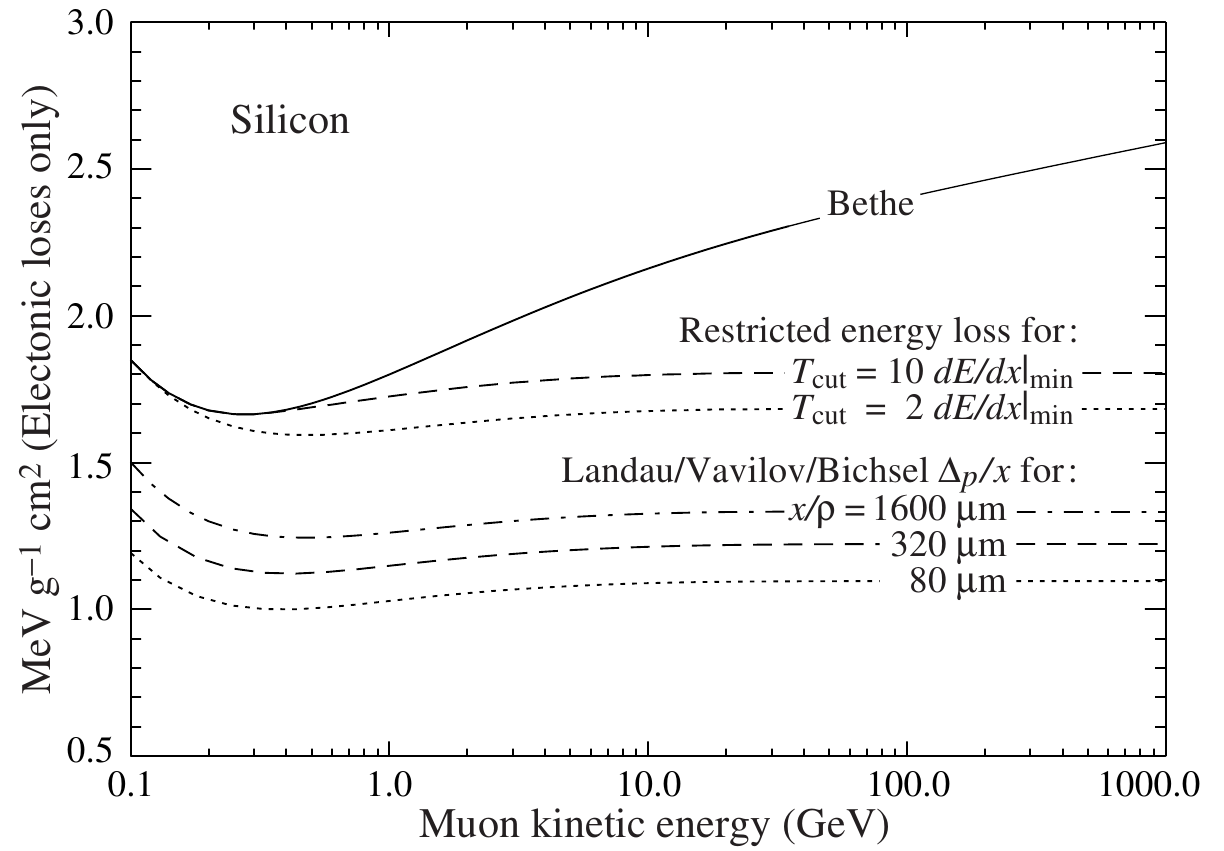
\includegraphics[width=0.6\textwidth]{figures/analysis/dEdx_Bethe_Landau.png}
  \end{tabular}
  \caption{Comparison between the Bethe mean energy loss, restricted energy loss and the most probable energy loss described by the Landau-Vavilov-Bichsel function for muons for different values of absorber thickness of silicon. Taken from \cite{bib:PDG_2014}.} 
  \label{fig:dEdx_Bethe_Landau}
\end{figure}
%However, it is difficult to determine the most probable value for tracks with only a few energy measurements available.
%Large fluctuations can still lead to a bias towards higher value of the most probable \dedx.

Particles such as  muons are minimally ionising in silicon for $\beta\gamma \sim 3-4$. 
For higher momenta the deposited energies increase again reaching a plateau at around $\beta\gamma\sim100$. 
However, new heavy charged particles would mainly be unrelativistic because of their high mass and would therefore deposit much higher energies in the detector.
This makes \dedx  a very well discriminating variable.
%\begin{figure}[!bt]
%  \centering 
%  \begin{tabular}{c}
%  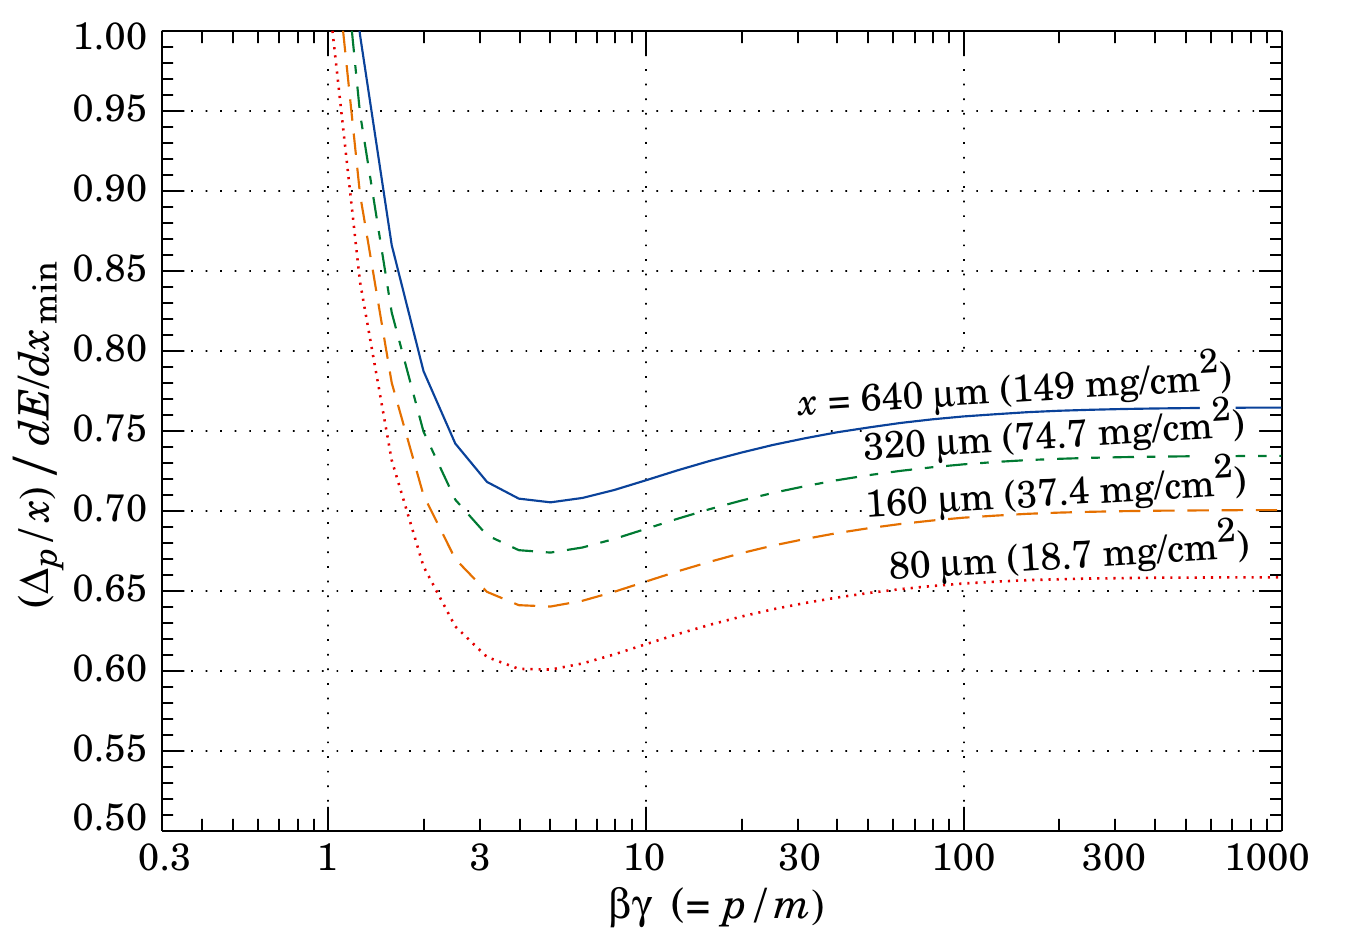
\includegraphics[width=0.6\textwidth]{figures/analysis/dEdx_Landau_Silicon.png}
%  \end{tabular}
%  \caption{Most probable energy loss in silicon, scaled to the mean loss of a minimally ionising particle (388 eV/$\mu$m) for different absorber thicknesses. Taken from \cite{bib:PDG_2014}.} 
%  \label{fig:dEdx_Landau_Silicon}
%\end{figure}
Thus, the energy loss per path length can be used to discriminate between SM particles and new heavy charged particles due to the different velocity distributions.\\

As said before, the most probable energy loss is much more stable compared to the Bethe mean energy loss.
Still, combining only a few measurments of $\Delta E/\Delta x$ can also lead for $\Delta_p/dx$ to large fluctuations towards high \dedx values.
In order to estimate experimentally the most probable \dedx value from only a few energy measurements, several ``estimators'' can be used that suppress a potential bias towards the high end without introducing a bias towards lower values~\cite{bib:Quertenmont_2010}.
One of the estimators for determining a tracks's \dedx is the harmonic-2 estimator
\begin{equation}
\ihtwo=\left( \frac{1}{N}\sum_{i=1}^{N}(\Delta E_i/\Delta x_i)^{-2} \right)^{-1/2},
\label{eq:Harmonic2Estimator}
\end{equation}
where $\Delta E_i /\Delta x_i$ corresponds to the $\Delta E$ and $\Delta x$ measurement in the $i$th hit of the track. 
This estimator is known to be robust and not be easily biased by large fluctions in  $\Delta E/\Delta x$ because of the supression by a factor of two.
%The harmonic mean of all $N$ measurements to the power of two is used as estimator for the MPV of the \dedx distribution of a particle.

The harmonic-2 estimator is also used for the pixel energy calibration described in the following section.


\FloatBarrier
\section{Energy calibration of the silicon pixel tracker}
\label{sec:EnergyCalibration}
During Run I in 2012, the pixel silicon detector was continuously subjected to an energy calibration, a so-called gain calibration.
Every pixel was calibrated to the same response, so that the whole pixel tracker should have been well inter-calibrated~\cite{bib:Danek}.
Unfortunately, due to various reasons, such as the imperfect constancy of the reference signal, or radiation and temperature induced changes, the energy calibration could not ensure a fully calibrated pixel tracker.
%was not adequate enough to use the measured energy deposition without a further offline calibration procedure.
This imperfection of the gain calibration can be seen in Fig.~\ref{fig:StabilityPlot_beforeCalibration}, where the mean of the harmonic-2 estimator for all tracks $\langle\ihtwo \rangle$ over the full data-taking period in 2012 is shown.
Four different steps can be spotted.
\begin{figure}[!b]
  \centering 
  \begin{tabular}{c}
  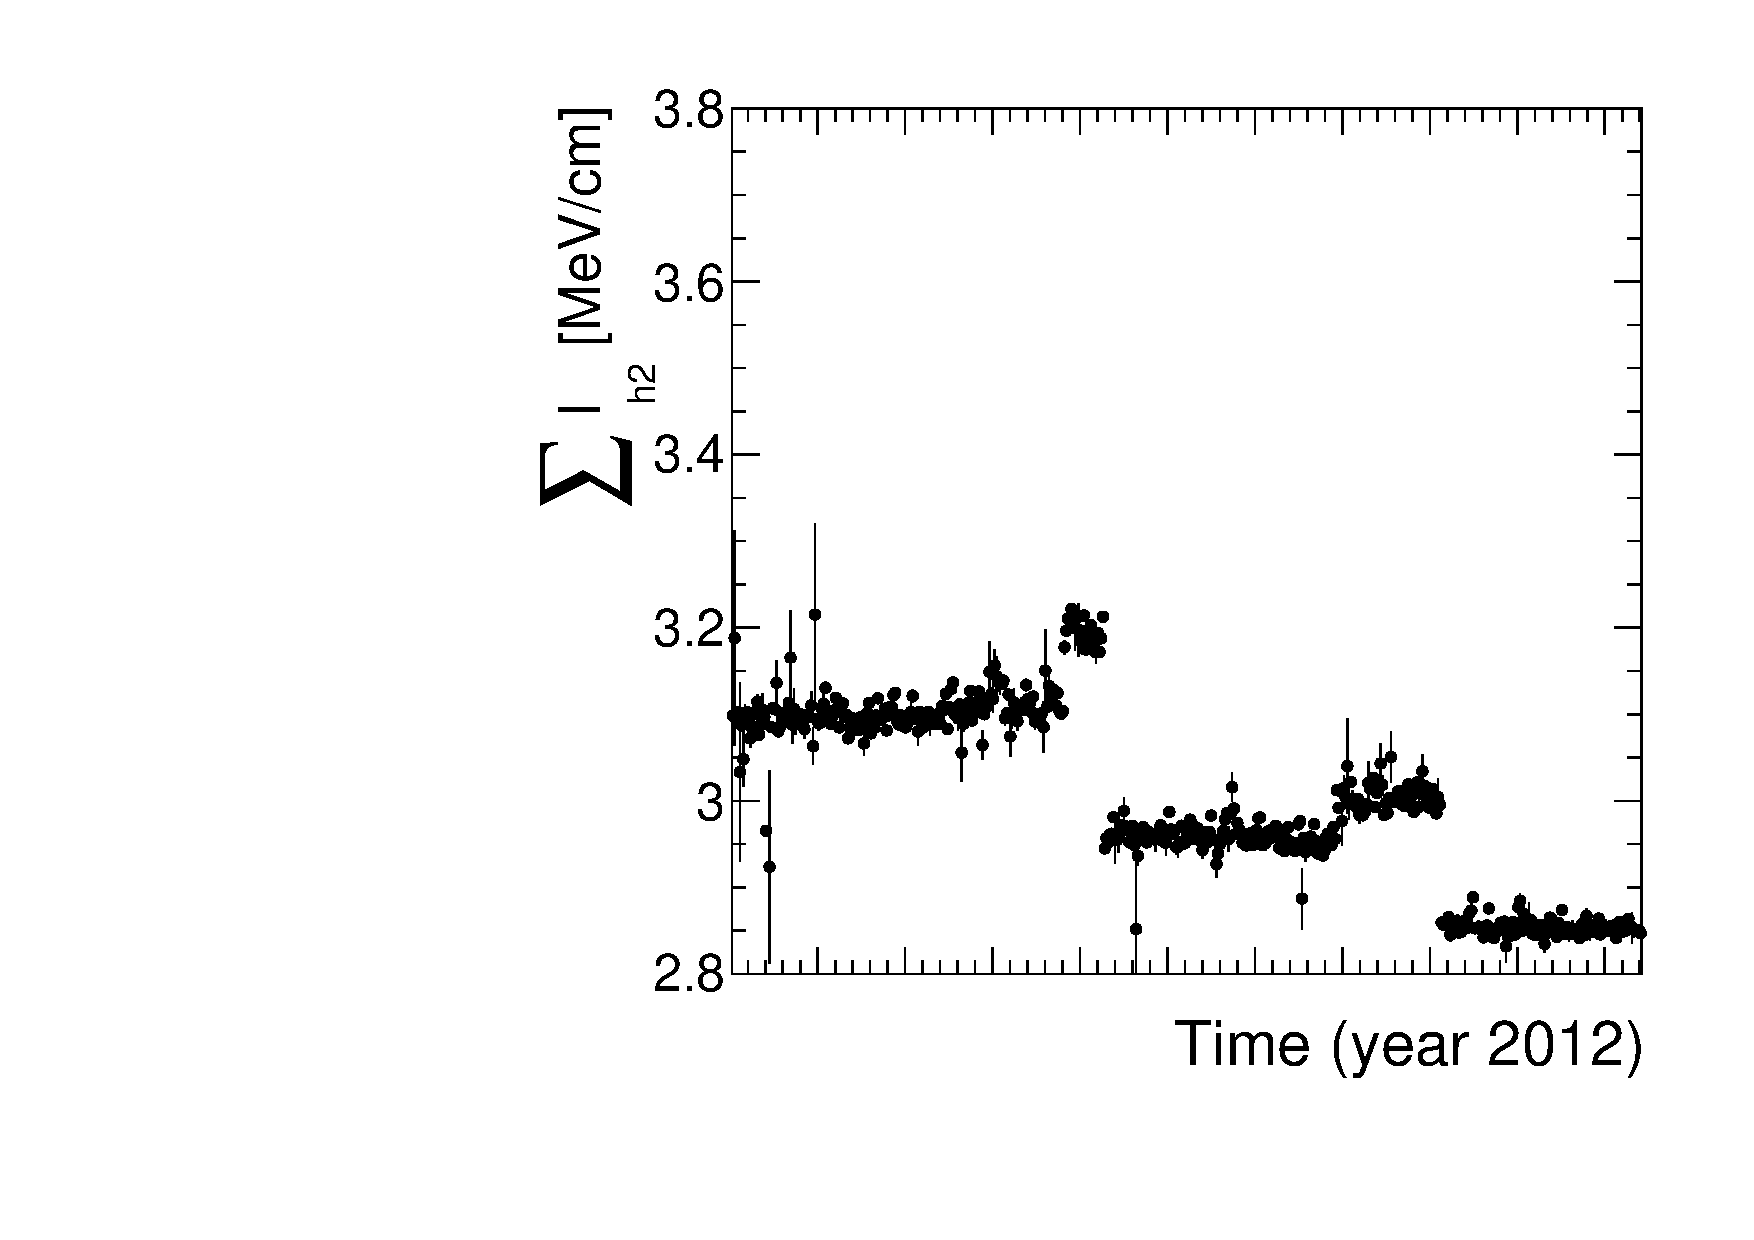
\includegraphics[width=0.49\textwidth]{figures/analysis/PixelCalibration/StabilityPlot_Pixel_beforeCalibration_withoutStepFits_NEW.pdf}
  \end{tabular}
  \caption{Mean of all track's \dedx (harmonic-2 estimator) over the full year 2012. Only pixel hits are taken into account. Every data point corresponds to one run.} 
  \label{fig:StabilityPlot_beforeCalibration}
\end{figure}
The first and the third steps correspond to changes in the settings of the tracker due to irradiation.
The second and fourth step are induced by associated adjustments in the online gain calibration.
Unfortunately, although the gain calibration was adjusted (even with some delay), it was not able to ensure a constant energy response of the pixel tracker over time. 
The variations of the \dedx measurement over time of around 15\% are too large to use \dedx without a further calibration. 

The following sections explain the method of the gain calibration of the pixel silicon tracker which is conducted for this analysis. 
It is splitted into two sections. 
The first section is dedicated to the gain inter-calibration of the pixel tracker which ensures a homogenious energy response of all tracker modules.
In the second section, the absolute gain calibration is discussed. 
This calibration step is needed to ensure that the measurement of the energy realease of a particle is actually translated to the correct physical value.

Detailed technical information about the pixel tracker can be found in Section~\ref{sec:Detector:Pixel}.


\subsection*{Inter-calibration of gain}
The main goal of the gain calibration is to get a uniform response in the ionisation energy loss \dedx over the full data taking period in 2012.
To also ensure a uniform response over all modules within one time step, an additional inter-calibration on module level is carried out.
The inter-calibration can in principle be done on various levels: the highest granularity would be a calibration on pixel level, followed by a calibration on read-out-chip (ROC) level and then on module-level.
Lower granularities in descending order are rings (modules with same z-position) and finally layers (3 layers in the barrel and 4 disks in the endcap). 
It is checked that all pixels and all ROCs (on one module) are well inter-calibrated, such that the inter-calibration is finally done module-wise.
%The applied method for the gain calibration of the pixel tracker closely follows the method in \cite{bib:Quertenmont_2010}.

The gain calibration of the pixel silicon tracker is carried out with the help of minimally ionising particles (MIPs).
MIPs in this context are not defined as particles depositing a minimum amount of energy, but more generally a small amount of energy.
This denotes all particles located at or near the plateau of the most probable \dedx distribution vs. momentum (see Fig.~\ref{fig:dEdx_Landau_Silicon}).
This approach ensures that all particles deposit similar amounts of energy so that the variation due to different momenta is minimised.
MIPs are selected by a momentum selection of $\text{p}>2\,$\gev.
Additionally, only tracks with at least eight hits and a $\chi^2/\text{n.d.o.f.}<3$ are used to ensure a high-quality track reconstruction.
A sample containing around $~$50 million ``minimum bias'' events is used for calibration.
The ``minimum bias'' sample was specifically recorded for tracker calibration purposes.
Its distinctive property is that neither an online nor offline selection was applied.

For every module in the pixel tracker (there are 1440 modules in total), a distribution of the energy loss per path length $\Delta E/\Delta x$ is built.
The measurement of $\Delta E/\Delta x$ is done in ADC counts per mm.
ADC counts are a measure for the deposited charge after digitisation.
%each $\Delta E/\Delta x$  measurement of all particles crossing the module is filled into a histogram. 
Figure~\ref{fig:dEdx_Module} shows an example distribution for one module.
\begin{figure}[!bt]
  \centering 
  \begin{tabular}{c}
  \includegraphics[width=0.49\textwidth]{figures/analysis/Landau_Module_352476680.pdf}
  \end{tabular}
  \caption{An example of the $\Delta E/\Delta x$ distribution measured in ADC count per mm for one module of the CMS pixel tracker. 
           A Landau convoluted with a Gaussian is fitted to the core of the distribution in an iterative procedure.} 
  \label{fig:dEdx_Module}
\end{figure}
The underlying Landau distribution can be nicely seen. 
To extract the MPV for every module a fit to the core distribution is performed.
The fit is not only done with a Landau but a Landau convoluted with a Gaussian function to be closer to the experimentally observed energy spectrum.
This also increases the fit performance and the stability of the fit.
The path length $\Delta x$ is calculated with
\begin{equation*}
\Delta x = d_{\text{module}_i} \cdot \cos(\phi_{\text{track}}),
\end{equation*}
where $d_{\text{module}_i}$ is the thickness of module i and $\phi_{\text{track}}$ is the relative angle of the particle's trajectory to the normal axis of the module.
With the measured MPV extracted from the fit, an inter-calibration factor is calculated for every module
\begin{equation*}
c_{\text{inter}}=\frac{\mpv_{\text{target}}\, [\text{ADC/mm}]}{\mpv\, [\text{ADC/mm}]} = \frac{300 \cdot 265 \, \text{ADC/mm}}{\mpv\, [\text{ADC/mm}]}.
\end{equation*}
The factor 300 $\cdot$ 265 ADC/mm is in principal an arbitrary number since the final response is adjusted by the absolute gain calibration described in the next section.
However, it is chosen such that the measured calibration factors are close to one.
The calibration factor can then be used to scale every single measurement in a module to a calibrated $\Delta E/\Delta x$ measurement
\begin{equation*}
\frac{\Delta E}{\Delta x}_{\text{calibrated}}=c_{\text{inter}} \cdot \frac{\Delta E}{\Delta x}_{\text{uncalibrated}}
\end{equation*}
The determination of the calibration factor is done for every of the five time steps, shown in Fig.~\ref{fig:StabilityPlot_beforeCalibration} independently, in order to get rid of the time dependency. 
The outcome of the application of the calibration factors to the single energy measurements in the pixel tracker can be seen in Fig.~\ref{fig:StabilityPlot_afterCalibration}.
The variation over time is indeed eliminated, resulting in a maximal time variation of less than $\sim1$\%.
\begin{figure}[!bt]
  \centering 
  \begin{tabular}{c}
  \includegraphics[width=0.49\textwidth]{figures/analysis/PixelCalibration/StabilityPlot_Pixel_afterCalibration_withoutStepFits_NEW.pdf}
  \end{tabular}
  \caption{Sum of all track's \dedx (harmonic-2 estimator) over the full year 2012 after applying the calibration factors, resulting in an average \dedx of 3.51 MeV/cm. Only pixel hits are taken into account. Every data point corresponds to one run.} 
  \label{fig:StabilityPlot_afterCalibration}
\end{figure}

Additionally, the same procedure is carried out for a corresponding simulated data sample to ensure the inter-calibration of the pixel modules on all simulated samples.




\subsection*{Absolute calibration of gain}
As a final step, the targeted \mpv being $\mpv_{\text{target}}=300 \cdot 265 \,  \text{ADC/mm}$ needs to be translated to a meaningful physical quantity given in physical units (\eg MeV/cm).
That means, that the charge measurement in ADC counts needs to be converted to the real energy release of a particle.
The relation between $\Delta E$ in ADC counts and the energy loss in eV is given by
\begin{equation}
\Delta E\,[\ev] = c_{\text{inter}} \cdot \Delta E\,[\text{ADC}] \cdot \frac{N_e}{\text{ADC}} \cdot 3.61 \, \ev,
\end{equation}
where $N_e$/ADC is the number of electrons which correspond to one calibrated ADC count and 3.61\,\ev is the  mean energy needed to create one electron-hole pair in silicon at -10$\degree$C.
Such an absolute gain calibration can be done with the help of several methods (all explained in \cite{bib:Quertenmont_2010}).
The absolute calibration of the silicon pixel tracker can rely on the already conducted absolute calibration of the silicon strip detector.
In \cite{bib:Quertenmont_2010}, the absolute gain calibration was done with the help of the most probable energy release per path length of muons, 
theoretically described by the Landau-Vavilov-Bichsel formula in Eq.~\eqref{eq:Landau_Vavilov_Bichsel}.  
To calibrate the pixel tracker to the correct energy loss per path length it is therefore sufficient to determine one calibration factor to relate the average \dedx of all tracks in the pixel tracker as shown in 
Fig.~\ref{fig:StabilityPlot_afterCalibration} to the average measured \dedx in the strip tracker, shown in Fig.~\ref{fig:StabilityPlot_Strip} by
\begin{equation}
c_{\text{absolute}} = \frac{\langle dE/dx_{\text{strip}} \rangle}{\langle dE/dx_{\text{pixel}} \rangle} = \frac{3.303}{3.509} = 0.941.
\end{equation}
\begin{figure}[!bt]
  \centering 
  \begin{tabular}{c}
  \includegraphics[width=0.49\textwidth]{figures/analysis/PixelCalibration/StabilityPlot_Strip_afterCalibration_withoutStepFits_NEW.pdf}
  \end{tabular}
  \caption{Mean of all track's \dedx (harmonic-2 estimator) measured in the silicon strip detector over the full year 2012. The average most probable \dedx is $\ihtwo=3.303\,\mev/\cm$. Every data point corresponds to one run.} 
  \label{fig:StabilityPlot_Strip}
\end{figure}
This factor is then applied on top of $c_{\text{inter}}$ for all pixel modules.

Finally, an absolute calibration factor needs to be determined for the simulated samples, where the simulated pixel tracker is calibrated to the average \dedx of the silicon strip measured in data.

\section{Discrimination of highly-ionising particles}
\label{sec:Ias}

As mentioned before, it is difficult to find a robust estimator for the most probable energy loss of a particle, if only a few measurements of $\Delta E/ \Delta x$  along the particle's trajectory are available.
The harmonic-2 estimator \ihtwo was already introduced in Section~\ref{sec:sub:MeasuringDeDx} in Eq.~\eqref{eq:Harmonic2Estimator}.
It is known to be a robust estimator not easily affected by large fluctuations in $\Delta E/ \Delta x$.
However, it was shown in \cite{bib:Quertenmont_2010} that a better discrimination between SM particles and possible new heavy particles can be achieved when using likelihood techniques,
\ie determining the probability that the set of all $\Delta E/ \Delta x$ belonging to one track is actually compatible with the hypothetical probability distribution of a MIP.

That a measured sample has been drawn from a specific distribution can be tested with the co-called Smirnov-Cram\'{e}r-von Mises test~\cite{bib:Anderson:CramerVonMises_1962,bib:James:StaticticalMethods_2006}.
It is deduced from the integral of the squared difference of the measured distribution $P_N(x)$ to the hypothesis distribution $P(x)$
\begin{equation}
I_s = \int\limits_{-\infty}^{\infty} \left[P_{N}(x)-P(x)\right]^2 dP(x)
\end{equation}
leading to a test statistics of
\begin{equation}
I_s = \frac{3}{N} \cdot \left( \frac{1}{12N} + \sum\limits_{i=1}^N \left[ P_i - \frac{2i-1}{2N} \right]^2 \right),
\end{equation}
where N is the total number of energy measurements and $P_i$ is the cumulative probability that a MIP would release a $\Delta E/\Delta x$ equal or smaller than the measured $\Delta E/ \Delta x$ with all $P_i$ arranged in increasing order.

However, this test statistics is not sensitive to the sign of the difference between the measured and the theoretical distribution.
It can therefore not distinguish between incompatibilities due to variations towards higher or lower energy deposits compared to the hypothesis distribution.
Thus it is not suitable for the discrimination between MIPs and heavy new particles by \dedx.
A so-called Asymmetric Smirnov-Cram\'{e}r-von Mises discriminator was developed in \cite{bib:Quertenmont_2010} which is only sensitive to incompatibilities to the MIP hypothesis towards higher energy depositions
\begin{equation}
\ias = \frac{3}{N} \cdot \left( \frac{1}{12N} + \sum\limits_{i=1}^N \left[ P_i \cdot \left(P_i - \frac{2i-1}{2N} \right)^2 \right] \right).
\end{equation}
A value of \ias close to zero indicates good compatibility with the MIP hypothesis, whereas a value close to one indicates bad compatibility because of unexpectedly high energy losses.

The underlying probability P$_i$ of the energy release for a given path length in the pixel tracker is extracted from the same ``Minimum bias'' sample used for the pixel energy calibration.
In total 28 different templates each for a different given path length are created.
In Fig.~\ref{fig:ProbabilityTemplate} the probability distribution template for the pixel tracker in data and simulation is shown.
The corresponding templates for the energy release in the silicon strip detector were already built by  \cite{bib:Quertenmont_2010}.


A comparison between the energy release by MIPs (\ias) in data and simulation for high-quality tracks with $p>5\gev$ and $|\eta|<2.1$ can be found in Fig.~\ref{fig:Data-MC-Dedx_MIPs}.
\begin{figure}[!tb]
  \centering 
  \begin{tabular}{c}
    \includegraphics[width=0.49\textwidth]{figures/analysis/Discriminator_template_data_pixel_2012.png}
    \includegraphics[width=0.49\textwidth]{figures/analysis/Discriminator_template_mc_pixel_2012.png}
  \end{tabular}
  \caption{Cumulative probability for a MIP to release a $\Delta E/ \Delta x$ (y-axis) vs. the path length (x-axis) in data (left) and simulation (right) for the pixel tracker based on the ``Minimum bias'' sample.}
  \vspace{60pt}
  \label{fig:ProbabilityTemplate}
\end{figure}

\begin{figure}[!bt]
\vspace{10pt}
  \centering 
  \begin{tabular}{c}
    \includegraphics[width=0.49\textwidth]{figures/analysis/PixelCalibration/htrackASmiSmallRange_log_MIPs.pdf}
  \end{tabular}
  \caption{Normalised \ias distribution for MIPs from the minimum bias sample in data and simulation for high-quality (high purity as defined in \cite{bib:CMS:Tracking_2010}, a minimum number of eight hits and no missing inner and middle hits) tracks with $p>5\gev$ and $|\eta|<2.1$.}
  \label{fig:Data-MC-Dedx_MIPs}
\end{figure}
\dedx shows good agreement in data and simulation for $\ias<0.1$.
For larger values, \ias shows a larger decrease in simulation than in measured data.
For this reason a data-based approach for analyses exploiting \dedx information is needed.\\

\section{Discrimination improvements}
\label{sec:DiscriminationImprovements}
The goal of including the pixel energy information is to increase the discrimination power of \ias between background and signal tracks, especially for shorter lifetimes.
In Fig.~\ref{fig:MIPs-Signal-Dedx}, a comparison of the shapes of the energy release by MIPs and by signal tracks in simulation is shown (details about the simulated samples can be found in the next section Section~\ref{sec:SignalSamples}).
\begin{figure}[!b]
  \centering 
  \begin{tabular}{c}
    \includegraphics[width=0.49\textwidth]{figures/analysis/PixelCalibration/htrackASmiSmallRange_log_chiTracksGoodQualitySelection_2Signal_ttjets.pdf}   
    \includegraphics[width=0.49\textwidth]{figures/analysis/PixelCalibration/htrackASmiSmallRange_log_chiTracksGoodQualitySelection_4Signal.pdf}
  \end{tabular}
  \caption{Normalised \ias distribution for simulated background and signal tracks (left) and for four different signal models (right) 
           for high-purity tracks (as defined in \cite{bib:CMS:Tracking_2010}) with \pt$>10\gev$ and $|\eta|<2.1$.
           For the illustration of the background tracks' spectrum simulated $t\bar{t}$+jets events are used (more information about this sample is given in Section~\ref{sec:SimulatedSamples}).}
  \label{fig:MIPs-Signal-Dedx}
\end{figure} 
It can be seen, that the \ias distributions of all signal models show a larger tail towards $\ias=1$, whereas the \ias of the background is rapidly falling.
The \ias distribution is not only influenced by the velocity ($\beta$) of a particle but also by the number of hits of a track.
The influence of the velocity can be easily seen in Eq.~\eqref{eq:Landau_Vavilov_Bichsel}. 
This in turn results in a dependency of \ias on the mass of the incident particle.
However, also for charginos with same mass, the velocity is higher in average for shorter lifetimes.
This is caused by the fact, that for shorter lifetimes (\eg $\ctau=10\cm$), already a sizable fraction of the charginos decay before reaching the tracker system.
The probability of reaching the detector increases for higher velocities because of the boost, which can be clearly seen at the survival probability
\begin{equation}
P \left( t \right) = e^{-\frac{t}{\gamma \tau}}.
\end{equation} 
This means that the track reconstruction/selection lead to a biased average $\beta$ for shorter lifetimes which in turn lead to lower values of \ias.

The number of measurements in the tracker system defines the influence of single fluctuations in $\Delta E/\Delta x$ on the \ias discriminator, because of the long right tail of the Landau distribution, A low number of hits lead therefore to higher \ias values.

Thus, \ias for charginos with lower lifetimes are affected by two things: 
First, due to the smaller number of measurements the chargino tends to higher \ias values.
Second, low lifetimes charginos have in average a higher velocity leading to lower \ias values.
Both effects can be seen in Fig.~\ref{fig:MIPs-Signal-Dedx} (right).
The large tail for longer lifetimes is caused by the lower velocities, but the small surplus between 0.1 and 0.2 is caused by the smaller number of measurements for lower lifetimes.\\


Finally, the impact of the additional $\Delta E/\Delta x$ information from the pixel tracker on the selection efficiency of signal and background tracks is quantified.
Figure~\ref{fig:ROCplots} shows the signal selection efficiency against the background selection efficiency for different selection cuts in \ias, once including the pixel information and once without it.
\begin{figure}[!b]
  \centering 
  %\vspace{79pt}
  \begin{tabular}{c}
    \includegraphics[width=0.49\textwidth]{figures/analysis/rocplot_wjets_mass_100GeV_ctau_5cm.pdf} 
    \includegraphics[width=0.49\textwidth]{figures/analysis/rocplot_wjets_mass_100GeV_ctau_50cm.pdf} \\
    \includegraphics[width=0.49\textwidth]{figures/analysis/rocplot_wjets_mass_500GeV_ctau_5cm.pdf} 
    \includegraphics[width=0.49\textwidth]{figures/analysis/rocplot_wjets_mass_500GeV_ctau_50cm.pdf}
  \end{tabular}
  \caption{Signal selection efficiency vs. background selection efficiency with (red) and without (black) pixel information.
           Each point correspond to one selection cut in \ias.
           The figure is based on a simulated \WJets sample and a simulated signal sample with chargino-chargino production, both subject to a selection of high-quality tracks (without a selection on \nhits) with $\pt>10\gev$.
       }
  %\vspace{40pt}
  \label{fig:ROCplots}
\end{figure} 
The background selection efficiency is estimated with simulated $W$+jets  events but was additionally checked on simulated $t\bar{t}$+jets  and QCD-multijet events 
(further information about the simulated samples can be found in the next section).
No significant difference between these processes in the background selection efficiency was observed.

The signal selection efficiency and the background suppression depend on the mass and the lifetime of the charginos.
The discrimination power of \ias is much better for higher masses as expected.

It can be seen that the inclusion of the pixel information increases the background suppression for a given signal efficiency throughout the investigated signal models.
This background suppression improvement is most pronounced for very tight cuts on \ias (up to a factor of 20) and still considerable for looser selections with signal efficiencies of around 40\% (factor of 10).


%%%%%%%%%%%%%%%%%%%%%%%%%%%%%%%%%%%%%%%%%%%%%%%%%%%%%%%%%%%%%%%%%%%%%%%%%%%%%%%%%%%%%%%%%%%%%%%%%%%%%%%%%%%%%%%%%%%%%%%%%%%%%%%%%%%%%%%%%%%%%%%%%%%%%%%%%%%%%%%%%%%%%%%%%%%%%%%%%%%%
%%%%%%%%%%%%%%%%%%%%%%%%%%%%%%%%%%%%%%%%%%%%%%%%%%%%%%%%%%%%%%%%%%%%%%%%%%%%%%%%%%%%%%%%%%%%%%%%%%%%%%%%%%%%%%%%%%%%%%%%%%%%%%%%%%%%%%%%%%%%%%%%%%%%%%%%%%%%%%%%%%%%%%%%%%%%%%%%%%%%

  %%%%%%%%%%%%%%%%%%%%%%%%%%%%%%%%%%%%%%%%%%%%%%%%%%%%%%%%%%%%%%%%%%%%%%%%%%%%%%%%%%%%%%%%%%%%%%%%%%%%%%%%%%%%%%%%%%%%%%%%%%%%%%%%%%%%%%%%%%%%%%%%%%%%%%%%%%%%%%%%%%%%%%%%%%%%%%%%%%%%
%%%%%%%%%%%%%%%%%%%%%%%%%%%%%%%%%%%%%%%%%%%%%%%%%%%%%%%%%%%%%%%%%%%%%%%%%%%%%%%%%%%%%%%%%%%%%%%%%%%%%%%%%%%%%%%%%%%%%%%%%%%%%%%%%%%%%%%%%%%%%%%%%%%%%%%%%%%%%%%%%%%%%%%%%%%%%%%%%%%%
%%%%%%%%%%%%%%%%%%%%%%%%%%%%%%%%%%%%%%%%%%%%%%%%%%%%%%%%%%%%%%%%%%%%%%%%%%%%%%%%%%%%%%%%%%%%%%%%%%%%%%%%%%%%%%%%%%%%%%%%%%%%%%%%%%%%%%%%%%%%%%%%%%%%%%%%%%%%%%%%%%%%%%%%%%%%%%%%%%%%
\FloatBarrier
\chapter{Improved dE/dx measurement for short tracks}
\label{sec:DeDxMeasurement}
As already pointed out in the previous chapter, the inclusion of the pixel energy measurements can increase the sensitivity when searching for short and highly ionising tracks.
While the energy measurements in the silicon strip detector have already been calibrated as part of the search for long-lived charged particles \cite{bib:CMS:HSCP_8TeV}, no complete calibration has been done for the pixel silicon tracker so far.
To increase the discrimination power of \dedx for short tracks, such a calibration procedure is therefore conducted within this PhD thesis.

The CMS tracker system provides a measurement of the particle's energy loss for each hit in the tracker.
This is done by the detection of the number of electrons produced by the ionisation of the silicon.
A detailed introduction to the CMS tracker system and the energy measurement can be found in Section~\ref{FIXME}.

How to combine the single energy measurements for each tracker hit into one track \dedx estimator that can be used for analysis purposes will be explained in the following Section~\ref{sec:sub:MeasuringDeDx}.
The pixel energy calibration is then described in Section~\ref{sec:EnergyCalibration}. 
How to discriminate SM particles and beyond SM particles with the help of a \dedx measurement is discussed in Section~\ref{sec:Ias}, followed by an exploration of how the inclusion of the pixel energy measurements in the \dedx estimates leads to a better discrimination between Standard Model particles and long-lived charginos (Section~\ref{sec:DiscriminationImprovements}).

%The CMS tracker system does not only allow for the precise measurement of particle tracks and primary and secondary vertices but also the measurement of a particle's mean energy loss per path length.
%This is done by the detection of the number of electrons produced by the ionisation of the particle during its passage through the silicon tracker.
%A detailed introduction to the CMS tracker system and the energy measurement can be found in Section~\ref{FIXME}.

%It was already pointed out that the inclusion of the pixel energy measurements can increase the sensitivity when searching for short and highly ionising tracks.
%While the silicon strip detector has already been calibrated as part of the search for long-lived charged particles \cite{bib:CMS:HSCP_8TeV}, no complete calibration has been done for the pixel silicon tracker so far.
%To increase the discrimination power of \dedx for short tracks, such a calibration procedure is therefore conducted within this PHD thesis.


\section{Estimation of the ionisation loss of charged particles}
\label{sec:sub:MeasuringDeDx}
Energy losses for moderately relativistic charged particles travelling through matter are mostly caused by ionisation effects.
The mean energy loss per path length can be described with the Bethe formula \cite{bib:Bethe_1930}:
\begin{equation}
\langle \frac{dE}{dx} \rangle = Kz^2\frac{Z}{A}\frac{1}{\beta^2} [ \frac{1}{2} \ln{\frac{2m_e c^2 \beta^2 \gamma^2 T_{\text{max}}}{I^2}} - \beta^2 - \frac{\delta( \beta \gamma )}{2} ].
\end{equation}
It is a function of the atomic number ($Z$), the atomic mass ($A$) of the absorber, and the mean excitation energy ($I$) which is 173\,eV for silicon~\cite{bib:NIST}.  
$T_{\text{max}}$ represents the maximum energy transfer in a single collision.
The relevant particle's properties are the velocity ($\beta$), the Lorentz factor ($\gamma$) and the charge (z) of the incident particle.
The density correction $\delta( \beta \gamma )$ reduces the mean energy loss at high energies because of polarisation effects of the material. 
%The constant factor K is $4\pi N_A r_e^2 m_e^2 c^2$ with $N_A$ being the Avogadro constant, $m_e$ the electron mass and $r_e$ the classical electron radius of 2.8\,fm.
The factor K is constant and is 0.307 in units of $\mev\,$mol$^{-1}$cm$^2$.
The Bethe formula is valid if the main energy loss originates from ionisation effects, \ie in a region between $0.1\lesssim\beta\gamma\lesssim 1000$.


Even if widely used, the mean energy loss is a quantity which is ``ill-defined experimentally and is not useful for describing energy loss by single particles'' \cite{bib:PDG_2014}.
The problem is caused by the underlying probability distribution of one single \dedx measurement (this will be named $\Delta E/ \Delta x $ throughout the following sections), which can be parametrised by a Landau distribution \cite{bib:Landau_1944}
\begin{equation}
p(x) = \frac{1}{\pi} \int_0^\infty\! e^{-t \log t - x t} \sin(\pi t)\, dt.
\end{equation}
The Landau distribution has no free parameters. Its most probable value is around 0.222.
However, it is possible to introduce artificially a different most probable value and a width (at half maximum) with $x \rightarrow \frac{x-\text{MPV}}{\sigma}-0.222$.
The Landau distribution is a highly asymmetric distribution with a long tail towards the right end (see Fig.~\ref{fig:landau}).
\begin{figure}[!b]
  \centering 
  \begin{tabular}{c}
  \includegraphics[width=0.49\textwidth]{figures/analysis/PixelCalibration/Landau.pdf}
  \end{tabular}
  \caption{Illustration of the shape of a Landau distribution. Parameters were chosen as $\mu=200$ and $\sigma=20$.} 
  \label{fig:landau}
\end{figure}
Theoretically it extends to infinite energies, however in nature the maximal deposited energy is of course limited by the particle's full energy.
%The mean and the variance of a landau distribution are not defined.

Because of its strong asymmetry, measurements of the mean energy loss per path length $\langle \dedx \rangle$ with only a few single measurements are easily fluctuating towards high values.
This makes the use of the mean energy loss described by the Bethe formula for the discrimination of new heavy particles problematic, because fluctuations to high values reduce the discrimination power against massive particles which release in general higher amounts of energy in matter.
%This is again different for a (limited) measurment, as there it is always possible to calucalute a mean.
%Still, this leads to the fact that the definition of the mean energy loss per path length is a problematic and unstable concept.


A much better observable is the most probable value (MPV) of the Landau distribution.
The MPV is much more stable compared to the mean and is not as easily fluctuating to higher \dedx values. 
The most probable energy loss of a charged particle, $\Delta_p$, can be described by the Landau-Vavilov-Bichsel equation \cite{bib:Bichsel:MPV_1988}:
\begin{equation}
\Delta_p = \xi \left[ \ln \frac{2m_e c^2\beta^2\gamma^2}{I}  + \ln\frac{\xi}{I} + j - \beta^2 - \delta(\beta\gamma)  \right],
\label{eq:Landau_Vavilov_Bichsel}
\end{equation}
with $\xi=(K/Z)\langle Z/A \rangle (x/\beta^2)$. 
The thickness of the absorber $x$ appears explicitly in the Landau-Vavilov-Bichsel equation making the most probable energy loss per path \mbox{length $\Delta_p/dx$} logarithmically dependent on $x$.
A comparison between the Bethe mean energy loss $\langle \dedx \rangle$ and the most probable energy loss $\Delta_p/dx$ for muons is shown in Fig.~\ref{fig:dEdx_Bethe_Landau}.
\begin{figure}[!bt]
  \centering 
  \begin{tabular}{c}
  \includegraphics[width=0.6\textwidth]{figures/analysis/dEdx_Bethe_Landau.png}
  \end{tabular}
  \caption{Comparison between the Bethe mean energy loss, restricted energy loss and the most probable energy loss described by the Landau-Vavilov-Bichsel function for muons for different values of absorber thickness of silicon. Taken from \cite{bib:PDG_2014}.} 
  \label{fig:dEdx_Bethe_Landau}
\end{figure}
%However, it is difficult to determine the most probable value for tracks with only a few energy measurements available.
%Large fluctuations can still lead to a bias towards higher value of the most probable \dedx.

Particles such as  muons are minimally ionising in silicon for $\beta\gamma \sim 3-4$. 
For higher momenta the deposited energies increase again reaching a plateau at around $\beta\gamma\sim100$. 
However, new heavy charged particles would mainly be unrelativistic because of their high mass and would therefore deposit much higher energies in the detector.
This makes \dedx  a very well discriminating variable.
%\begin{figure}[!bt]
%  \centering 
%  \begin{tabular}{c}
%  \includegraphics[width=0.6\textwidth]{figures/analysis/dEdx_Landau_Silicon.png}
%  \end{tabular}
%  \caption{Most probable energy loss in silicon, scaled to the mean loss of a minimally ionising particle (388 eV/$\mu$m) for different absorber thicknesses. Taken from \cite{bib:PDG_2014}.} 
%  \label{fig:dEdx_Landau_Silicon}
%\end{figure}
Thus, the energy loss per path length can be used to discriminate between SM particles and new heavy charged particles due to the different velocity distributions.\\

As said before, the most probable energy loss is much more stable compared to the Bethe mean energy loss.
Still, combining only a few measurements of $\Delta E/\Delta x$ can also lead for $\Delta_p/dx$ to large fluctuations towards high \dedx values.
In order to estimate experimentally the most probable \dedx value from only a few energy measurements, several ``estimators'' can be used that suppress a potential bias towards the high end without introducing a bias towards lower values~\cite{bib:Quertenmont_2010}.
One of the estimators for determining a track's \dedx is the harmonic-2 estimator
\begin{equation}
\ihtwo=\left( \frac{1}{N}\sum_{i=1}^{N}(\Delta E_i/\Delta x_i)^{-2} \right)^{-1/2},
\label{eq:Harmonic2Estimator}
\end{equation}
where $\Delta E_i /\Delta x_i$ corresponds to the $\Delta E$ and $\Delta x$ measurement in the $i$th hit of the track. 
This estimator is known to be robust and not be easily biased by large fluctuations in  $\Delta E/\Delta x$ because of the suppression by the power of minus two.
%The harmonic mean of all $N$ measurements to the power of two is used as estimator for the MPV of the \dedx distribution of a particle.

%The harmonic-2 estimator is used for the pixel energy calibration described in the following section.


\FloatBarrier
\section{Energy calibration of the silicon pixel tracker}
\label{sec:EnergyCalibration}
During Run I in 2012, the pixel silicon detector was continuously subjected to an energy calibration, a so-called gain calibration.
Every pixel was calibrated to the same response, so that the whole pixel tracker should have been well inter-calibrated~\cite{bib:Danek}.
Unfortunately, due to various reasons, such as the imperfect constancy of the reference signal, or radiation and temperature induced changes, the energy calibration could not ensure a fully calibrated pixel tracker.
%was not adequate enough to use the measured energy deposition without a further offline calibration procedure.

This imperfection of the gain calibration can be seen in Fig.~\ref{fig:StabilityPlot_beforeCalibration}, where the mean of the harmonic-2 estimator for all tracks $\langle\ihtwo \rangle$ over the full data-taking period in 2012 is shown.
Four different steps can be spotted.
\begin{figure}[!b]
  \centering 
  \begin{tabular}{c}
  \includegraphics[width=0.49\textwidth]{figures/analysis/PixelCalibration/StabilityPlot_Pixel_beforeCalibration_withoutStepFits_NEW.pdf}
  \end{tabular}
  \caption{Mean of all track's \dedx (harmonic-2 estimator) over the full year 2012. Only pixel hits are taken into account. Every data point corresponds to one run.} 
  \label{fig:StabilityPlot_beforeCalibration}
\end{figure}
The first and the third steps correspond to changes in the settings of the tracker due to irradiation.
The second and fourth step are induced by associated adjustments in the online gain calibration.
Unfortunately, although the gain calibration was adjusted (even with some delay), it was not able to ensure a constant energy response of the pixel tracker over time. 
The variations of the \dedx measurement over time of around 15\% are too large to use \dedx without a further calibration. 

The following sections explain the method of the gain calibration of the pixel silicon tracker which is conducted for this analysis. 
It is splitted into two sections. 
The first section is dedicated to the gain inter-calibration of the pixel tracker which ensures a homogeneous energy response of all tracker modules.
In the second section, the absolute gain calibration is discussed. 
This calibration step is needed to ensure that the measurement of the energy release of a particle is actually translated to the correct physical value.

%Detailed technical information about the pixel tracker can be found in Section~\ref{sec:Detector:Pixel}.


\subsection*{Inter-calibration of gain}
The main goal of the gain calibration is to get a uniform response in the ionisation energy loss \dedx over the full data taking period in 2012.
To also ensure a uniform response over all modules within one time step, an additional inter-calibration on module level is carried out.
The inter-calibration can in principle be done on various levels: the highest granularity would be a calibration on pixel level, followed by a calibration on read-out-chip (ROC) level and then on module-level.
Lower granularities in descending order are rings (modules with same z-position) and finally layers (3 layers in the barrel and 4 disks in the endcap). 
It is verified that all pixels and all ROCs (on one module) are well inter-calibrated, such that the inter-calibration is finally done module-wise.

%The applied method for the gain calibration of the pixel tracker closely follows the method in \cite{bib:Quertenmont_2010}.

The gain calibration of the pixel silicon tracker is carried out with the help of minimally ionising particles (MIPs).
MIPs in this context are not defined as particles at the minimum of the Bethe formula, but more generally as particles located at or near the plateau of the \dedx distribution vs. momentum (see Fig.~\ref{fig:dEdx_Bethe_Landau}).
This approach ensures that all particles deposit similar amounts of energy so that the variation due to different momenta is minimised.

MIPs are selected by a momentum selection of $\text{p}>2\,$\gev.
Additionally, only tracks with at least eight hits and a $\chi^2/\text{n.d.o.f.}<3$ are used to ensure a high-quality track reconstruction.
A sample containing around $~$50 million ``minimum bias'' events is used for calibration.
The ``minimum bias'' sample was specifically recorded for tracker calibration purposes.
%Its distinctive property is that neither an online nor offline selection was applied.

For every module in the pixel tracker (there are 1440 modules in total), a distribution of the energy loss per path length $\Delta E/\Delta x$ is built.
The measurement of $\Delta E/\Delta x$ is done in ADC counts per mm.
ADC counts are a measure for the deposited charge after digitisation.
%each $\Delta E/\Delta x$  measurement of all particles crossing the module is filled into a histogram. 
Figure~\ref{fig:dEdx_Module} shows an example distribution for one module.
\begin{figure}[!t]
  \centering 
  \begin{tabular}{c}
  \includegraphics[width=0.49\textwidth]{figures/analysis/Landau_Module_352476680.pdf}
  \end{tabular}
  \caption{An example of the $\Delta E/\Delta x$ distribution measured in ADC count per mm for one module of the CMS pixel tracker. 
           A Landau convoluted with a Gaussian is fitted to the core of the distribution in an iterative procedure.} 
  \label{fig:dEdx_Module}
\end{figure}
The underlying Landau distribution can be nicely seen. 
To extract the MPV for every module a fit to the core distribution is performed.
The fit is not only done with a Landau but a Landau convoluted with a Gaussian function to be closer to the experimentally observed energy spectrum.
This also increases the fit performance and the stability of the fit.
The path length $\Delta x$ is calculated with
\begin{equation}
\Delta x = d_{\text{module}_i} \cdot \cos(\phi_{\text{track}}),
\end{equation}
where $d_{\text{module}_i}$ is the thickness of module i and $\phi_{\text{track}}$ is the relative angle of the particle's trajectory to the normal axis of the module.
With the measured MPV extracted from the fit, an inter-calibration factor is calculated for every module

\begin{equation}
c_{\text{inter}}=\frac{\mpv_{\text{target}}\, [\text{ADC/mm}]}{\mpv\, [\text{ADC/mm}]} = \frac{300 \cdot 265 \, \text{ADC/mm}}{\mpv\, [\text{ADC/mm}]}.
\end{equation}

The factor 300 $\cdot$ 265 ADC/mm is in principal an arbitrary number since the final response is adjusted by the absolute gain calibration described in the next section.
However, it is chosen such that the measured calibration factors are close to one.
The calibration factor can then be used to scale every single measurement in a module to a calibrated $\Delta E/\Delta x$ measurement

\begin{equation}
\left( \frac{\Delta E}{\Delta x}\right)_{\text{calibrated}}=c_{\text{inter}} \cdot \left(\frac{\Delta E}{\Delta x}\right)_{\text{uncalibrated}}
\end{equation}

The determination of the calibration factor is done for every of the five time steps, shown in Fig.~\ref{fig:StabilityPlot_beforeCalibration} independently, in order to get rid of the time dependency. 
The outcome of the application of the calibration factors to the single energy measurements in the pixel tracker can be seen in Fig.~\ref{fig:StabilityPlot_afterCalibration}.
The variation over time is indeed eliminated, resulting in a maximal time variation of less than $\sim1$\%.

\begin{figure}[!t]
  \centering 
  \begin{tabular}{c}
  \includegraphics[width=0.49\textwidth]{figures/analysis/PixelCalibration/StabilityPlot_Pixel_afterCalibration_withoutStepFits_NEW.pdf}
  \end{tabular}
  \caption{Mean of all track's \dedx (harmonic-2 estimator) over the full year 2012 after applying the calibration factors, resulting in an average \dedx of 3.51 MeV/cm. Only pixel hits are taken into account. Every data point corresponds to one run.} 
  \label{fig:StabilityPlot_afterCalibration}
\end{figure}


Additionally, the same procedure is carried out for a corresponding simulated data sample to ensure the inter-calibration of the pixel modules on all simulated samples.



\subsection*{Absolute calibration of gain}
As a final step, the targeted \mpv being $\mpv_{\text{target}}=300 \cdot 265 \,  \text{ADC/mm}$ needs to be translated to a meaningful physical quantity given in physical units (\eg MeV/cm).
That means, that the charge measurement in ADC counts needs to be converted to the real energy release from a particle.
The relation between $\Delta E$ in ADC counts and the energy loss in eV is given by
\begin{equation}
\Delta E\,[\ev] = c_{\text{inter}} \cdot \Delta E\,[\text{ADC}] \cdot \frac{N_e}{\text{ADC}} \cdot 3.61 \, \ev,
\end{equation}
where $N_e$/ADC is the number of electrons which correspond to one calibrated ADC count and 3.61\,\ev is the  mean energy needed to create one electron-hole pair in silicon at -10$\degree$C.
Such an absolute gain calibration can be done with the help of several methods (all explained in \cite{bib:Quertenmont_2010}).
The absolute calibration of the silicon pixel tracker can rely on the already conducted absolute calibration of the silicon strip detector.
In \cite{bib:Quertenmont_2010}, the absolute gain calibration was done with the help of the most probable energy release per path length of muons, 
theoretically described by the Landau-Vavilov-Bichsel formula in Eq.~\eqref{eq:Landau_Vavilov_Bichsel}.  
To calibrate the pixel tracker to the correct energy loss per path length it is therefore sufficient to determine one calibration factor to relate the average \dedx of all tracks in the pixel tracker as shown in 
Fig.~\ref{fig:StabilityPlot_afterCalibration} to the average measured \dedx in the strip tracker, shown in Fig.~\ref{fig:StabilityPlot_Strip} by
\begin{equation}
c_{\text{absolute}} = \frac{\langle dE/dx_{\text{strip}} \rangle}{\langle dE/dx_{\text{pixel}} \rangle} = \frac{3.303}{3.509} = 0.941.
\end{equation}
\begin{figure}[!b]
  \centering 
  \begin{tabular}{c}
  \includegraphics[width=0.49\textwidth]{figures/analysis/PixelCalibration/StabilityPlot_Strip_afterCalibration_withoutStepFits_NEW.pdf}
  \end{tabular}
  \caption{Mean of all track's \dedx (harmonic-2 estimator) measured in the silicon strip detector over the full year 2012. The average most probable \dedx is $\ihtwo=3.303\,\mev/\cm$. Every data point corresponds to one run.} 
  \label{fig:StabilityPlot_Strip}
\end{figure}
This factor is then applied on top of $c_{\text{inter}}$ for all pixel modules.

Finally, an absolute calibration factor needs to be determined for the simulated samples, where the simulated pixel tracker is calibrated to the average \dedx of the silicon strip measured in data.

\section{Discrimination of highly-ionising particles}
\label{sec:Ias}

As mentioned before, it is difficult to find a robust estimator for the most probable energy loss of a particle, if only a few measurements of $\Delta E/ \Delta x$  along the particle's trajectory are available.
The harmonic-2 estimator \ihtwo was already introduced in Section~\ref{sec:sub:MeasuringDeDx} in Eq.~\eqref{eq:Harmonic2Estimator}.
It is known to be a robust estimator not easily affected by large fluctuations in $\Delta E/ \Delta x$.
However, it was shown in \cite{bib:Quertenmont_2010} that a better discrimination between SM particles and possible new heavy particles can be achieved when using likelihood techniques,
\ie determining the probability that the set of all $\Delta E/ \Delta x$ belonging to one track is actually compatible with the hypothetical probability distribution of a MIP.

That a measured sample has been drawn from a specific distribution can be tested with the co-called Smirnov-Cram\'{e}r-von Mises test~\cite{bib:Anderson:CramerVonMises_1962,bib:James:StaticticalMethods_2006}.
%It is deduced from the integral of the squared difference of the measured distribution $P_N(x)$ to the hypothesis distribution $P(x)$
It is deduced from the integral of the squared difference of a measured distribution to a hypothesis distribution, 
%\begin{equation}
%I_s = \int\limits_{-\infty}^{\infty} \left[P_{N}(x)-P(x)\right]^2 dP(x)
%\end{equation}
and leads to a test statistics of~\cite{bib:Quertenmont_2010}
\begin{equation}
I_s = \frac{3}{N} \cdot \left( \frac{1}{12N} + \sum\limits_{i=1}^N \left[ P_i - \frac{2i-1}{2N} \right]^2 \right),
\end{equation}
where N is the total number of energy measurements and $P_i$ is the cumulative probability that a MIP would release a $\Delta E/\Delta x$ equal or smaller than the measured $\Delta E/ \Delta x$ with all $P_i$ arranged in increasing order.

However, this test statistics is not sensitive to the sign of the difference between the measured and the theoretical distribution.
It can therefore not distinguish between incompatibilities due to variations towards higher or lower energy deposits compared to the hypothesis distribution.
Thus it is not suitable for the discrimination between MIPs and heavy new particles by \dedx.
A so-called Asymmetric Smirnov-Cram\'{e}r-von Mises discriminator was developed in \cite{bib:Quertenmont_2010} which is only sensitive to incompatibilities to the MIP hypothesis towards higher energy depositions
\begin{equation}
\ias = \frac{3}{N} \cdot \left( \frac{1}{12N} + \sum\limits_{i=1}^N \left[ P_i \cdot \left(P_i - \frac{2i-1}{2N} \right)^2 \right] \right).
\end{equation}
A value of \ias close to zero indicates good compatibility with the MIP hypothesis, whereas a value close to one indicates bad compatibility because of unexpectedly high energy losses.

The underlying probability P$_i$ of the energy release for a given path length in the pixel tracker is extracted from the same ``minimum bias'' sample used for the pixel energy calibration.
In total 28 different templates each for a different given path length are created.
In Fig.~\ref{fig:ProbabilityTemplate} the probability distribution template for the pixel tracker in data and simulation is shown.
The corresponding templates for the energy release in the silicon strip detector were already built by  \cite{bib:Quertenmont_2010}.


A comparison between the energy release by MIPs (\ias) in data and simulation for high-quality tracks with $p>5\gev$ and $|\eta|<2.1$ can be found in Fig.~\ref{fig:Data-MC-Dedx_MIPs}.
\begin{figure}[!tb]
  \centering 
  \begin{tabular}{c}
    \includegraphics[width=0.49\textwidth]{figures/analysis/PixelCalibration/Discriminator_template_data_pixel_2012.png}
    \includegraphics[width=0.49\textwidth]{figures/analysis/PixelCalibration/Discriminator_template_mc_pixel_2012.png}
  \end{tabular}
  \caption{Cumulative probability for a MIP to release a $\Delta E/ \Delta x$ (y-axis) vs. the path length (x-axis) in data (left) and simulation (right) for the pixel tracker based on the ``minimum bias'' sample.}
  \vspace{60pt}
  \label{fig:ProbabilityTemplate}
\end{figure}

\begin{figure}[!bt]
\vspace{10pt}
  \centering 
  \begin{tabular}{c}
    \includegraphics[width=0.49\textwidth]{figures/analysis/PixelCalibration/htrackASmiSmallRange_log_MIPs.pdf}
  \end{tabular}
  \caption{Normalised \ias distribution for MIPs from the minimum bias sample in data and simulation for high-quality (high purity as defined in \cite{bib:CMS:Tracking_2010}, a minimum number of eight hits and no missing inner and middle hits) tracks with $p>5\gev$ and $|\eta|<2.1$.}
  \label{fig:Data-MC-Dedx_MIPs}
\end{figure}
\dedx shows good agreement in data and simulation for $\ias<0.1$.
For larger values, \ias shows a larger decrease in simulation than in measured data.
For this reason a data-based approach for analyses exploiting \dedx information is needed.\\

\section{Discrimination improvements}
\label{sec:DiscriminationImprovements}
The goal of including the pixel energy information is to increase the discrimination power of \ias between background and signal tracks, especially for shorter lifetimes.
In Fig.~\ref{fig:MIPs-Signal-Dedx} (left), a comparison of the shapes of the energy release by MIPs and by signal tracks in simulation is shown (details about the simulated samples can be found in the next section Section~\ref{sec:SignalSamples}).
\begin{figure}[!b]
  \centering 
  \begin{tabular}{c}
    \includegraphics[width=0.49\textwidth]{figures/analysis/PixelCalibration/htrackASmiSmallRange_log_chiTracksGoodQualitySelection_2Signal_ttjets.pdf}   
    \includegraphics[width=0.49\textwidth]{figures/analysis/PixelCalibration/htrackASmiSmallRange_log_chiTracksGoodQualitySelection_4Signal.pdf}
  \end{tabular}
  \caption{Normalised \ias distribution for simulated background and signal tracks (left) and for four different signal models (right) 
           for high-purity tracks (as defined in \cite{bib:CMS:Tracking_2010}) with \pt$>10\gev$ and $|\eta|<2.1$.
           For the illustration of the background tracks' spectrum simulated $t\bar{t}$+jets events are used (more information about this sample is given in Section~\ref{sec:SimulatedSamples}).}
  \label{fig:MIPs-Signal-Dedx}
\end{figure} 
It can be seen, that the \ias distributions of the signal models show a larger tail towards $\ias=1$, whereas the \ias of the background is rapidly falling.

In the right part of Fig.~\ref{fig:MIPs-Signal-Dedx}, a comparison of four different signal models is shown.
Charginos with longer lifetimes have a more pronounced tail toward $\ias=1$.
This can be understood with the help of Eq.~\eqref{eq:Landau_Vavilov_Bichsel}, where the influence of the velocity ($\beta$) on the ionisation loss can be seen.
The velocity distribution of the charginos is mostly affected by the mass of the chargino.
However, also for charginos with same mass, the velocity is higher in average for shorter lifetimes.
This is caused by the fact, that for shorter lifetimes (\eg $\ctau=10\cm$), already a sizable fraction of the charginos decay before reaching the tracker system.
The probability of reaching the detector increases for higher velocities because of the boost, which can be clearly seen at the survival probability
\begin{equation}
P \left( t \right) = e^{-\frac{t}{\gamma \tau}}.
\end{equation} 
This means that the track reconstruction/selection lead to a biased average $\beta$ for shorter lifetimes which in turn lead to lower values of \ias.

The \ias distribution is not only influenced by the velocity of a particle but also by the number of hits of a track.
The number of measurements in the tracker system defines the influence of single fluctuations in $\Delta E/\Delta x$ on the \ias discriminator, because of the long right tail of the Landau distribution.
A low number of hits lead therefore to higher \ias values.
This effect is also visible Fig.~\ref{fig:MIPs-Signal-Dedx} (right) by the small surplus for lower lifetimes between 0.1 and 0.2 is caused by the smaller number of measurements for earlier decaying charginos.

%Thus, \ias for charginos with lower lifetimes are affected by two things: 
%First, due to the smaller number of measurements the chargino tends to higher \ias values.
%Second, low lifetimes charginos have in average a higher velocity leading to lower \ias values.
%Both effects can be seen in Fig.~\ref{fig:MIPs-Signal-Dedx} (right).
%The large tail for longer lifetimes is caused by the lower velocities, but the small surplus for lower lifetimes between 0.1 and 0.2 is caused by the smaller number of measurements for earlier decaying charginos.\\


Finally, the impact of the additional $\Delta E/\Delta x$ information from the pixel tracker on the selection efficiency of signal and background tracks is quantified.
Figure~\ref{fig:ROCplots} shows the signal selection efficiency against the background selection efficiency for different selection cuts in \ias, once including the pixel information and once without it.
\begin{figure}[!b]
  \centering 
  %\vspace{79pt}
  \begin{tabular}{c}
    \includegraphics[width=0.49\textwidth]{figures/analysis/rocplot_wjets_mass_100GeV_ctau_5cm.pdf} 
    \includegraphics[width=0.49\textwidth]{figures/analysis/rocplot_wjets_mass_100GeV_ctau_50cm.pdf} \\
    \includegraphics[width=0.49\textwidth]{figures/analysis/rocplot_wjets_mass_500GeV_ctau_5cm.pdf} 
    \includegraphics[width=0.49\textwidth]{figures/analysis/rocplot_wjets_mass_500GeV_ctau_50cm.pdf}
  \end{tabular}
  \caption{Signal selection efficiency vs. background selection efficiency with (red) and without (black) pixel information.
           Each point correspond to one selection cut in \ias.
           The figure is based on a simulated \WJets sample and a simulated signal sample with chargino-chargino production, both subject to a selection of high-quality tracks (without a selection on \nhits) with $\pt>10\gev$.
       }
  %\vspace{40pt}
  \label{fig:ROCplots}
\end{figure} 
The background selection efficiency is estimated with simulated $W$+jets  events but was additionally checked on simulated $t\bar{t}$+jets  and QCD-multijet events 
(further information about the simulated samples can be found in the next section).
No significant difference between these processes in the background selection efficiency was observed.

The signal selection efficiency and the background suppression depend on the mass and the lifetime of the charginos.
The improvement of the discriminating power is much more pronounced for higher chargino masses.

It can be seen that the inclusion of the pixel information increases the background suppression for a given signal efficiency throughout the investigated signal models.
This background suppression improvement is most pronounced for very tight cuts on \ias up to a factor of 20 and even more and still considerable for looser selections with signal efficiencies of around 40\% (factor of 10).
%%%%%%%%%%%%%%%%%%%%%%%%%%%%%%%%%%%%%%%%%%%%%%%%%%%%%%%%%%%%%%%%%%%%%%%%%%%%%%%%%%%%%%%%%%%%%%%%%%%%%%%%%%%%%%%%%%%%%%%%%%%%%%%%%%%%%%%%%%%%%%%%%%%%%%%%%%%%%%%%%%%%%%%%%%%%%%%%%%%%
%%%%%%%%%%%%%%%%%%%%%%%%%%%%%%%%%%%%%%%%%%%%%%%%%%%%%%%%%%%%%%%%%%%%%%%%%%%%%%%%%%%%%%%%%%%%%%%%%%%%%%%%%%%%%%%%%%%%%%%%%%%%%%%%%%%%%%%%%%%%%%%%%%%%%%%%%%%%%%%%%%%%%%%%%%%%%%%%%%%%

  %%%%%%%%%%%%%%%%%%%%%%%%%%%%%%%%%%%%%%%%%%%%%%%%%%%%%%%%%%%%%%%%%%%%%%%%%%%%%%%%%%%%%%%%%%%%%%%%%%%%%%%%%%%%%%%%%%%%%%%%%%%%%%%%%%%%%%%%%%%%%%%%%%%%%%%%%%%%%%%%%%%%%%%%%%%%%%%%%%%%
%%%%%%%%%%%%%%%%%%%%%%%%%%%%%%%%%%%%%%%%%%%%%%%%%%%%%%%%%%%%%%%%%%%%%%%%%%%%%%%%%%%%%%%%%%%%%%%%%%%%%%%%%%%%%%%%%%%%%%%%%%%%%%%%%%%%%%%%%%%%%%%%%%%%%%%%%%%%%%%%%%%%%%%%%%%%%%%%%%%%
\section{Simulated samples}
\label{sec:SimulatedSamples}

For the investigation of the various backgrounds to this search, the analysis relies also on simulated sample.
An extensive introduction to the techniques and tools required for the simulation of SM and beyond SM processes can be found in Section~\ref{FIXME}.

In the following two sections an overview about the used SM (Section~\ref{sec:SMSamples}) and SUSY samples (Section~\ref{sec:SignalSamples}) is given.
All samples are reweighted to match the measured distribution of primary vertices in data.

\subsection{SM Background samples}
\label{sec:SMSamples}
To investigate the sources of background, various simulated SM samples were used.
In order to have the possibility to make use of the $dE/dx$ variables, a special data format of the simulated samples is required (called RECO format).
Unfortunately, not all SM processes were available in this format in which also the information about the energy release in the tracking system is included.
However, as this analysis needs to rely anyways on a data-based background estimation method, because of the limited quality of the $dE/dx$ simulation.
this does not constitute a serious problem, but only limit the possibility of an extensive comparison between data and simulation going beyond shape comparisons.

In Table \ref{tab:SMsamples_RECO} all SM samples are listed which were available in the RECO format and are used in the analysis.
\renewcommand{\arraystretch}{1.5}
\begin{table}[!b]
\centering
\caption{Available and used Standard Model background samples containing $\Delta E/\Delta x$ information.}
\label{tab:SMsamples_RECO}
\makebox[0.99\textwidth]{
\begin{tabular}{lll}
\multicolumn{3}{c}{} \\
\toprule
 Process & Cross section $\left[\pb\right]$ & $\mathcal{O}_{\text{calculation}}$ \\%& Size $\left[\text{TB}\right]$\\
\midrule
 $W$ + jets                                             &  36703.2     &  NNLO \cite{bib:FEWZ} \\%& 70.4 \\
 $t\bar{t}$ + jets                                      &  245.8       &  NNLO \cite{bib:ttbar:Czakon_2013}\\%& 55.9 \\
 Z$\rightarrow\ell\ell$ ($\ell=e,\mu,\tau$)             &  3531.9      &  NNLO \cite{bib:FEWZ} \\%& 5.1  \\
 QCD ($50\gev<\hat{p}_{\text{T}}<1400\gev$)               &  9374794.2    &  LO  \\%% & 44.3\\
\bottomrule
\end{tabular}}
\end{table}  
Due to the immense size of the samples (between 5 and 70\,TB) and in order to match a reasonable storage space a reduction was done by selecting only events which contain at least one leading jet with a minimum transverse momentum of $\pt>60\gev$.

In addition, further simulated samples not containing the energy information are used.
These are needed to study the backgound inclusively in the variable \ias.
They are listed in Table~\ref{tab:SMsamples_AOD}.
\renewcommand{\arraystretch}{1.5}
\begin{table}[!t]
\centering
\caption{Used Standard Model background samples without $\Delta E/\Delta x$ information.}
\label{tab:SMsamples_AOD}
\makebox[0.99\textwidth]{
\begin{tabular}{lll}
\multicolumn{3}{c}{} \\
\toprule
 Process & Cross section $\left[\pb\right]$ & $\mathcal{O}_{\text{calculation}}$ \\%& Size $\left[\text{TB}\right]$\\
\midrule
 $W$ + jets                                                &  36703.2    &  NNLO \cite{bib:FEWZ} \\%& 70.4 \\
 Z$\rightarrow\ell\ell$ ($\ell=e,\mu,\tau$) + 1,2,3,4 jets &  3531.9     &  NNLO \cite{bib:FEWZ} \\%& 5.1  \\
\bottomrule
\end{tabular}}
\end{table}  

%\begin{itemize}
%\item Main Background are ... ???
%\item Most important sample was included: Wjets
%\item ZoNuNu Backgrund not availbale plays also a role (see DT paper!)
%\item Table of SM samples with cross sections
%\end{itemize}

\subsection{Signal samples}
\label{sec:SignalSamples}
For the investigation of a possible signal, events containing either chargino pair production $q\bar{q} \rightarrow \chipm \chimp$ or chargino neutralino production $q\bar{q} \rightarrow \chipm \chiO$ are simulated. 
The simulation is done with the matrix-element event generator \madgraph \cite{bib:Madgraph_2014}
The parton showering and hadronization processes are then simulated with Pythia 6 \cite{bib:Pyhtia6_2006}.
A last step is needed to simulate the interations of the generated particles with the detector material, which is done with \geant \cite{bib:Geant4_2003,bib:Geant4_2006}.

Furthermore, a speacial treatment for long-lived particles is required.
In order to get the right detector simulation of the energy loss of the long-lived particles which decay after the beam pipe, the lifetime of the chargino cannot be set in the matrix-element generator but needs to be specified within \geant.
This also means, that the decay products are only existing in the detector simulation, but are not accessible as particles in the event generators.


To narrow down the required computing sources, the simulation was only done for a few lifetimes (1\cm, 5\cm, 10\cm, 50\cm, 100\cm, 1\,000\cm and 10\,000\cm).
To get still a tight scan over the lifetime space, other lifetimes were generated using lifetime reweighting.
This can be done by determining for every event a weight which is depending on the individual proper lifetime of the chargino (in case of chargino pair production it depends on the individual lifetime of the two charginos).
The event weight is given by
\begin{equation*}
w = \prod_{i=1}^n \frac{\tau^{\text{gen}}}{\tau^{\text{target}}}\cdot  \exp \left[ t_i \cdot \left( \frac{1}{\tau^{\text{target}}} - \frac{1}{\tau^{\text{gen}}} \right) \right] ,
\end{equation*}
where $n$ is the  number of charginos in the event, $\tau^{\text{gen}}$ is the generated mean lifetime in the particle's rest frame and $t_i$ is the individual proper lifetime of the chargino. 
The resulting mean lifetime is then given by $\tau^{\text{target}}$. A derivation of this formula can be found in Appendix~\ref{blabla}.
With the reweighting procedure a tight covering of the lifetime space could be achieved with lifetimes of \ctau = $a\cdot10^{n}$ for $n$=0,1,2,3,4 and $a$=$\left[1,9\right]$.
Figure~\ref{blabla} shows the exponential distribution of the individual proper lifetime of the charginos after reweighting a simulated sample with $c\tau^{\text{gen}}=50\cm$ to a lifetime of $c\tau^{\text{target}}=10\cm$.
Fitting the exponential spectrum should result in the correct mean proper lifetime as parameter of the fit.
It can be seen, that the reweighting procedure can reproduce the targeted lifetime of 10\cm.
\begin{figure}[!t]
  \centering 
  \begin{tabular}{c}
    \includegraphics[width=0.49\textwidth]{figures/analysis/10cm.pdf}
  \end{tabular}
  \caption{Normalized distribution of the proper lifetime $d_{\text{lab}}/\left(\beta\gamma \right)$ of all charginos contained in a signal sample with a generated lifetime of $c\tau^{\text{gen}}=50\cm$ reweighted to a lifetime of $c\tau^{\text{target}}=10\cm$.}
  \label{fig:FeynmanDiagram}
\end{figure}


All samples were generated for different chargino masses always almost mass-degenerate to the lightest neutralino.
The mass gap between chargino and neutralino was set to 5\gev.
However, as this analysis does not make use of the other decay products and the lifetime is set in \geant, the mass gap does not play any role.
Six different masses from 100\gev to 600\gev are simulated.
This leads then to a total number of 42 signal samples.
In Table~\ref{tab:SignalCrossSections} the NLO-NLL cross sections at $\sqrt{s}=8\tev$ for $\chipm\chimp$ and $\chipm\chiO$ production 
with wino-like charginos and degeneracy between $m_{\chipm}$ and $m_{\chiO}$ are listed \cite{bib:SignalCrossSection_2012,bib:SignalCrossSection_2013}.
The cross section does not dependent on the lifetime of the chargino.
\renewcommand{\arraystretch}{1.5}
\begin{table}[!h]
\centering
\caption{Produced signal simulated samples with corresponding cross sections}
\label{tab:SignalCrossSections}
\makebox[0.99\textwidth]{
\begin{tabular}{lll}
\multicolumn{3}{c}{} \\
\toprule
 $m_{\chipm}\left[\gev\right]$ & $\sigma_{\chipm\chimp}\left[\pb\right]$  & $\sigma_{\chiO\chimp}\left[\pb\right]$ \\
\midrule
 100     &  5.8234     &  11.5132 \\
 200     &  0.37924    &  0.77661 \\
 300     &  0.06751    &  0.14176 \\
 400     &  0.01751    &  0.03758 \\
 500     &  0.00553    &  0.01205 \\
 600     &  0.00196    &  0.00431 \\
\bottomrule
\end{tabular}}
\end{table}  

%%%%%%%%%%%%%%%%%%%%%%%%%%%%%%%%%%%%%%%%%%%%%%%%%%%%%%%%%%%%%%%%%%%%%%%%%%%%%%%%%%%%%%%%%%%%%%%%%%%%%%%%%%%%%%%%%%%%%%%%%%%%%%%%%%%%%%%%%%%%%%%%%%%%%%%%%%%%%%%%%%%%%%%%%%%%%%%%%%%%
%%%%%%%%%%%%%%%%%%%%%%%%%%%%%%%%%%%%%%%%%%%%%%%%%%%%%%%%%%%%%%%%%%%%%%%%%%%%%%%%%%%%%%%%%%%%%%%%%%%%%%%%%%%%%%%%%%%%%%%%%%%%%%%%%%%%%%%%%%%%%%%%%%%%%%%%%%%%%%%%%%%%%%%%%%%%%%%%%%%%
\section{Event selection}
\label{sec:EventSelection}
\subsection{Datasets and triggers}
\begin{itemize}
\item Datasets and triggers used in the analysis
\item signal samples generated with Madgraph and pythia
\item They are decayed in Geant to only pions. Around ten different lifetimes were simulated
\item For other lifetimes: lifetime reweighting is done PLOT
\item For five diffenrent masses (100-500 GeV) 
\end{itemize}
\subsection{Preselection}
\begin{itemize}
\item Motivate different selection cuts
\item Reference DT search for most of them
\end{itemize}
\subsection{Main discriminating variables}
\begin{itemize}
\item dE/dx
\item pt
\item Show some MC signal bkg comparioson plots (only Wjets?)
\end{itemize}

%%%%%%%%%%%%%%%%%%%%%%%%%%%%%%%%%%%%%%%%%%%%%%%%%%%%%%%%%%%%%%%%%%%%%%%%%%%%%%%%%%%%%%%%%%%%%%%%%%%%%%%%%%%%%%%%%%%%%%%%%%%%%%%%%%%%%%%%%%%%%%%%%%%%%%%%%%%%%%%%%%%%%%%%%%%%%%%%%%%%
\section{Sources of backgrounds}
\label{sec:SourcesOfBackgrounds}
\begin{itemize}
\item Background consist of particles which make high energy deposits and are high pt
\item In general: Low background search
\end{itemize}
\subsection{Fake tracks}
\begin{itemize}
\item Definition of fake tracks
\item How can they fake the signal
\end{itemize}
\subsection{Muons}
\begin{itemize}
\item How can muons fake the signal
\end{itemize}
\subsection{Pions}
\begin{itemize}
\item How can pions fake the signal
\end{itemize}
\subsection{Electrons}
\begin{itemize}
\item How can electrons fake the signal
\end{itemize}
%%%%%%%%%%%%%%%%%%%%%%%%%%%%%%%%%%%%%%%%%%%%%%%%%%%%%%%%%%%%%%%%%%%%%%%%%%%%%%%%%%%%%%%%%%%%%%%%%%%%%%%%%%%%%%%%%%%%%%%%%%%%%%%%%%%%%%%%%%%%%%%%%%%%%%%%%%%%%%%%%%%%%%%%%%%%%%%%%%%%
%%%%%%%%%%%%%%%%%%%%%%%%%%%%%%%%%%%%%%%%%%%%%%%%%%%%%%%%%%%%%%%%%%%%%%%%%%%%%%%%%%%%%%%%%%%%%%%%%%%%%%%%%%%%%%%%%%%%%%%%%%%%%%%%%%%%%%%%%%%%%%%%%%%%%%%%%%%%%%%%%%%%%%%%%%%%%%%%%%%%
\section{Background estimation methods}
\label{sec:BackgroundEstimation}
\subsection{Fake background}
\subsection{Leptonic background}
\subsection{Systematic uncertainties}

%%%%%%%%%%%%%%%%%%%%%%%%%%%%%%%%%%%%%%%%%%%%%%%%%%%%%%%%%%%%%%%%%%%%%%%%%%%%%%%%%%%%%%%%%%%%%%%%%%%%%%%%%%%%%%%%%%%%%%%%%%%%%%%%%%%%%%%%%%%%%%%%%%%%%%%%%%%%%%%%%%%%%%%%%%%%%%%%%%%%
\section{Optimization of search sensitivity}
\label{sec:Optimization}
\begin{itemize}
\item Show plots
\item show table
\item Include NlostOuter here, too
\end{itemize}

%%%%%%%%%%%%%%%%%%%%%%%%%%%%%%%%%%%%%%%%%%%%%%%%%%%%%%%%%%%%%%%%%%%%%%%%%%%%%%%%%%%%%%%%%%%%%%%%%%%%%%%%%%%%%%%%%%%%%%%%%%%%%%%%%%%%%%%%%%%%%%%%%%%%%%%%%%%%%%%%%%%%%%%%%%%%%%%%%%%%
\section{Statistical Methods/ Limit setting}
\label{sec:LimitSetting}

%%%%%%%%%%%%%%%%%%%%%%%%%%%%%%%%%%%%%%%%%%%%%%%%%%%%%%%%%%%%%%%%%%%%%%%%%%%%%%%%%%%%%%%%%%%%%%%%%%%%%%%%%%%%%%%%%%%%%%%%%%%%%%%%%%%%%%%%%%%%%%%%%%%%%%%%%%%%%%%%%%%%%%%%%%%%%%%%%%%%
\section{Results}
\label{sec:Results}
\begin{itemize}
\item Data cutflowtable
\item Tables with results
\item One plot (4 bins: Prediction and data)
\end{itemize}

%%%%%%%%%%%%%%%%%%%%%%%%%%%%%%%%%%%%%%%%%%%%%%%%%%%%%%%%%%%%%%%%%%%%%%%%%%%%%%%%%%%%%%%%%%%%%%%%%%%%%%%%%%%%%%%%%%%%%%%%%%%%%%%%%%%%%%%%%%%%%%%%%%%%%%%%%%%%%%%%%%%%%%%%%%%%%%%%%%%%
\section{Interpretation}
\label{sec:Interpretation}
\subsection{Systematic uncertainties of simulated signal samples}
\subsection{Exclusion limits}
\begin{itemize}
\item 1-d limits
\item 2-d limits
\end{itemize}


  %%%%%%%%%%%%%%%%%%%%%%%%%%%%%%%%%%%%%%%%%%%%%%%%%%%%%%%%%%%%%%%%%%%%%%%%%%%%%%%%%%%%%%%%%%%%%%%%%%%%%%%%%%%%%%%%%%%%%%%%%%%%%%%%%%%%%%%%%%%%%%%%%%%%%%%%%%%%%%%%%%%%%%%%%%%%%%%%%%%%
\section{Characterisation and estimation of the Standard Model backgrounds}
\label{sec:BackgroundEstimation}
After the application of the candidate track selection explained in the previous section the background arising from Standard Model processes is dramatically reduced.
However, it still happens sometimes that a electron, muon or tau fails reconstruction, which will be explained in detail in the following section~\ref{sec:LeptonicBkg}.
Furthermore, there is the possibility that a track is reconstructed out of a set of hits which do not origin from only one single particle.
Such tracks will be called ``fake tracks'' in the following. 
Background tracks arising from wrong reconstruction will be explained in Sec.~\ref{sec:FakeBkg}

The composition of the background is shown in Fig.~\ref{fig:BkgComposition}.
\begin{figure}[!tb]
  \centering 
  \begin{tabular}{c}
    \includegraphics[width=0.49\textwidth]{figures/analysis/htrackgenParticleSmallRange_lin_chiTracksfullSelectionTrigger.pdf}
    \includegraphics[width=0.49\textwidth]{figures/analysis/htrackgenParticleSmallRange_lin_chiTracksfullSelectionPlusIasTrigger.pdf}
  \end{tabular}
  \caption{bla bla}
  \label{fig:BkgComposition}
\end{figure}
This composiiton can change significantly when imposing further selection cuts on \pt and \ias.
This, however, will be addressed during the optimisation procedure.
To get a feeling how the composition of the background is affected by further cuts on one of the main variable \ias, 
the background composition is shown in Fig~\ref{fig:BkgComposition} with the analysis selection plus an additional \ias cut of 0.5.
As can be already seen in this figure the fake background becomes more important when apply also a selection on \ias, 
especially because the fake background is not only present in \WJets events but essentially in all Standard Model processes with missing energy. \\

Still, also the leptonic background can be important.
This is not possible to study with simulation because of the lack of statistics.
Additionally, when the simulation is not fully correct in simulating the operativeness of every single detector module, the simulation could highly underestimate the leptonic background.
Thus, a data based background estimation approach is needed.

\subsection{Leptonic background}
\label{sec:LeptonicBkg}

The leptonic background of the presented search is caused by non-reconstructed leptons which undergo hence the lepton veto selection.
However, at least a non-reconstructed electron or tau should in principle deposit enough energy in the ECAL that it can still be vetoed by the calorimeter isolation requirement.
As muons don't deposit much energy in the ECAL, this reason does not hold for them.
In the following, the sources of the three different leptonic backgrounds shall be charectized.

\subsubsection*{Electrons}
To avoid the background source from unreconstructed electrons, all tracks pointing to a dead or noisy ecal cells are vetoed, as described in the previous section.
By this selection, almost all electrons are efficiently rejected.
In the simulated \WJets sample only one simulated event remain which pass all candidate track selection criteria and where the candidate track can be matched to generator-level electron .
This event is visualised in Fig~\ref{fig:LostElectron}. 
\begin{figure}[!tb]
  \centering 
  \begin{tabular}{c}
    \includegraphics[width=0.49\textwidth]{figures/analysis/Electron_lumi_279317_event_111637553.png}
  \end{tabular}
  \caption{Visualization of an $W\rightarrow e\nu_e$ event contributing to the SM background. 
           In light blue the generator-level particles $e$ and $\nu_e$ of the $W$ decay are shown. 
           The $\nu_e$, only weakly interacting does not show any signature in the detector, whereas the electron ($\pt\simeq 90\gev$) leaves a track (black line) with \mbox{$\pt\simeq 70\gev$} in the tracker. 
           No ECAL energy deposits in the direction of the electron are visible. 
           This is caused by the fact that the corresponding ECAL energy deposits were not read out in this event.
           An ISR jet ($\pt\simeq 230\gev$) causes the \met (read arrow) in the event. }
  \label{fig:LostElectron}
\end{figure}
In this event to energy deposits in the ECAL are read out, which suggests, that this ECAL tower was neither working properly in 2012.
Additionally, electrons might do much bremstrahlung and as a effect can change the direction significantly, such that the deposited energy in the ECAL is not matched to the electron.

\subsubsection*{Taus}
The tau background is contributing through the hadronic decay of a tau lepton to one charged pion $\tau\rightarrow\pi^{\pm}\nu$.
Unreconstructed taus have typically large mismeasured \pt.
Because of nuclear interactions in the tracker, they have typically short tracks and therefore easily mismeasured \pt.
Additionnaly, the pion already looses energy in the tracker which opens up the possibility surviving also the calorimeter isolation selection.
Such an event is shown in Fig.~\ref{fig:LostTau}.
Unfortunately, due to the short length of the track, these events can sometimes also survive an \ias cut, because of possibly large $dE/dx$ fluctions.
\begin{figure}[!tb]
  \centering 
  \begin{tabular}{c}
    \includegraphics[width=0.49\textwidth]{figures/analysis/LostTau_Lumi_60133_Event_24033837.png}
  \end{tabular}
  \caption{Visualization of a $W^{+}\rightarrow \tau^{+}\nu_{\tau} \rightarrow \pi^{+} \nu_{\tau}$ event contributing to the SM background. 
           In light blue the generator-level particles $\pi^{+}$ and $\nu_{\tau}$ are shown.
           The reconstructed track (black line) is very short because the pion interacts with the tracker material via the strong force.}
  \label{fig:LostTau}
\end{figure}

\subsubsection*{Muons}
Muons can fail reconstruction when they are pointing torward a bad cathode strip chamber.
This is taken into account in the candidate track selection.
However, some of the muons still fail reconstruction when they fall within the gap between stations 0 and 1 of the DT system at $\eta=0.25$.
The muon reconstruction efficiency drops from around 99\% to a value of around 94\% as shown in~\ref{jessicathesis}. 
This possibility is illustrated in a simulated event shown in Fig~\ref{fig:LostMuon}.
\begin{figure}[!tb]
  \centering 
  \begin{tabular}{c}
    \includegraphics[width=0.49\textwidth]{figures/analysis/LostMuon_Lumi_357583_Event_142918834.png}
  \end{tabular}
  \caption{Visualization of an $W\rightarrow \mu\nu_{\mu}$ event contributing to the SM background. 
           In light blue the generator-level particles $\mu$ and $\nu_{\mu}$ of the $W$ decay are shown. }
  \label{fig:LostMuon}
\end{figure}
In~\ref{jessicastheisi} events are rejected when the track is pointing in a region of $0.15<|\eta|<0.35$.
In this search, this cut was omitted to maximise signal acceptance. 
Due to the additional selection in \ias, muons are easily efficiently supressed.
E.g. in the event example shown in Fig~\ref{fig:LostMuon}, the muon has an \ias value of about 0.02.\\


In general, all leptons are rather minimal ionizing, especially muons and pions.
Electrons can more easily interact with the shell electrons of the tracker material, but still the \ias spectrum is quickly decreasing compared to the signal.
To have the possibility to make an optimisation in the two main discriminating variables \pt and \ias, the background estimation methods are designed to work for all different \pt and \ias selection cuts.
\begin{itemize}
\item Show ias plot for electrons, muons, taus seperately!
\item Explain background estimation method
\item with fake background (should be metioned before the leptonic background!!!!!)
\end{itemize} 



%%%%%%%%%%%%%%%%%%%%%%%%%%%%%%%%%%%%%%%%%%%%%%%%%%%%%%%%%%%%%%%%%%%%%%%%%%%%%%%%%%%%%%%%%%%%%%%%%%%%%%%%%%%%%%%%%%%%%%%%%%%%%%%%%%%%%%%%%%%%%%%%%%%%%%%%%%%%%%%%%%%%%%%%%%%%%%%%%%%%
\subsection{Fake background}
\label{sec:FakeBkg}

\begin{itemize}
\item Show plot with fake rate in different samples
\end{itemize}

\subsection{Systematic uncertainties}
\label{sec:SysUncertaintiesBkg}


\begin{itemize}
\item Background consist of particles which make high energy deposits and are high pt
\item In general: Low background search
\end{itemize}


\newpage
%%%%%%%%%%%%%%%%%%%%%%%%%%%%%%%%%%%%%%%%%%%%%%%%%%%%%%%%%%%%%%%%%%%%%%%%%%%%%%%%%%%%%%%%%%%%%%%%%%%%%%%%%%%%%%%%%%%%%%%%%%%%%%%%%%%%%%%%%%%%%%%%%%%%%%%%%%%%%%%%%%%%%%%%%%%%%%%%%%%%
%%%%%%%%%%%%%%%%%%%%%%%%%%%%%%%%%%%%%%%%%%%%%%%%%%%%%%%%%%%%%%%%%%%%%%%%%%%%%%%%%%%%%%%%%%%%%%%%%%%%%%%%%%%%%%%%%%%%%%%%%%%%%%%%%%%%%%%%%%%%%%%%%%%%%%%%%%%%%%%%%%%%%%%%%%%%%%%%%%%%
\section{Optimization of search sensitivity}
\label{sec:Optimization}
\begin{itemize}
\item Show plots
\item show table
\item Include NlostOuter here, too
\end{itemize}

%%%%%%%%%%%%%%%%%%%%%%%%%%%%%%%%%%%%%%%%%%%%%%%%%%%%%%%%%%%%%%%%%%%%%%%%%%%%%%%%%%%%%%%%%%%%%%%%%%%%%%%%%%%%%%%%%%%%%%%%%%%%%%%%%%%%%%%%%%%%%%%%%%%%%%%%%%%%%%%%%%%%%%%%%%%%%%%%%%%%
\section{Statistical Methods/ Limit setting}
\label{sec:LimitSetting}

%%%%%%%%%%%%%%%%%%%%%%%%%%%%%%%%%%%%%%%%%%%%%%%%%%%%%%%%%%%%%%%%%%%%%%%%%%%%%%%%%%%%%%%%%%%%%%%%%%%%%%%%%%%%%%%%%%%%%%%%%%%%%%%%%%%%%%%%%%%%%%%%%%%%%%%%%%%%%%%%%%%%%%%%%%%%%%%%%%%%
\section{Results}
\label{sec:Results}
\begin{itemize}
\item Data cutflowtable
\item Tables with results
\item One plot (4 bins: Prediction and data)
\end{itemize}

%%%%%%%%%%%%%%%%%%%%%%%%%%%%%%%%%%%%%%%%%%%%%%%%%%%%%%%%%%%%%%%%%%%%%%%%%%%%%%%%%%%%%%%%%%%%%%%%%%%%%%%%%%%%%%%%%%%%%%%%%%%%%%%%%%%%%%%%%%%%%%%%%%%%%%%%%%%%%%%%%%%%%%%%%%%%%%%%%%%%
\section{Interpretation}
\label{sec:Interpretation}
\subsection{Systematic uncertainties of simulated signal samples}
\subsection{Exclusion limits}
\begin{itemize}
\item 1-d limits
\item 2-d limits
\end{itemize}


  %%%%%%%%%%%%%%%%%%%%%%%%%%%%%%%%%%%%%%%%%%%%%%%%%%%%%%%%%%%%%%%%%%%%%%%%%%%%%%%%%%%%%%%%%%%%%%%%%%%%%%%%%%%%%%%%%%%%%%%%%%%%%%%%%%%%%%%%%%%%%%%%%%%%%%%%%%%%%%%%%%%%%%%
%%%%%%%%%%%%%%%%%%%%%%%%%%%%%%%%%%%%%%%%%%%%%%%%%%%%%%%%%%%%%%%%%%%%%%%%%%%%%%%%%%%%%%%%%%%%%%%%%%%%%%%%%%%%%%%%%%%%%%%%%%%%%%%%%%%%%%%%%%%%%%%%%%%%%%%%%%%%%%%%%%%%%%%
\chapter{Optimisation of the search sensitivity}
\label{sec:Optimisation}
Finally, having all background estimation methods in place, an optimisation procedure is conducted in order to increase the search sensitivity with respect to the signal models introduced in Section~\ref{sec:SignalSamples}.
The optimisation is done in the most sensitive variables, \pt and \ias (see Section~\ref{sec:Ias} for a definition and explanation of the Asymmetric Smirnov discriminator \ias).

In this optimisation, the full systematic uncertainty is taken into account, which includes statistical uncertainties arising from limited statistical precision of the samples used in the background estimation methods and the systematic uncertainties that are described in Section~\ref{sec:SysUncertaintiesBkg}.
In order to avoid unnecessary fine-tuning of the optimisation to the specific cross sections of the SUSY models and to keep the search as general as possible, 
the optimisation is not done by maximising  $S/\Delta B$ but by a minimisation of the cross section for which a 5$\sigma$ discovery is possible, \ie finding the optimal selection cuts for \pt and \ias for which the lowest possible cross section can be discovered
\begin{equation}
\label{eq:optimisation}
\frac{\sigma_{\text{min}}\cdot \mathcal{L}}{\Delta B} = \frac{\sigma_{\text{min}}\cdot \mathcal{L}}{\sqrt{ \left(\Delta B_{\text{stat}}\right)^2 + \left(\Delta B_{\text{sys}}\right)^2}} \geq 5.
\end{equation} 
In this formula, $\mathcal{L}$ is the integrated luminosity in 2012, $\sigma_{\text{min}}$ is the minimum cross section that can be discovered, $\Delta B_{\text{sys}}$ is the systematic uncertainty of the background prediction as explained above and 
$\Delta B_{\text{stat}}$ is the statistical uncertainty of the background prediction which is the 68\% one sided upper limit of a poisson distribution with $\mu = B$ estimated with the 
Neyman construction~\cite{bib:Neyman_1937,bib:PDG_2014}.\\

For a first qualitative estimation of the optimal selection cuts, general systematic uncertainties on the leptonic and the fake background of 100\% and 20\% respectively are imposed.
Uncertainties arising from limited statistical precision of the samples used for the background estimation are propagated consistently into formula~\ref{eq:optimisation}.
The results of this optimisation for two very different lifetimes (5\cm and 50\cm) and masses (100\gev and 500\gev) are visualised in Fig.~\ref{fig:optimisation}, where the minimum cross section that is possible to discover is shown in the $\pt-\ias$ plane.
\begin{figure}[!h]
  \centering 
  \vspace{50pt}
  \begin{tabular}{c}
    \includegraphics[width=0.49\textwidth]{figures/analysis/Optimisation/Madgraph_signal_mass_100_ctau_5cm_ECaloLe5_SOverDeltaBStatPlusSys.pdf} 
    \includegraphics[width=0.49\textwidth]{figures/analysis/Optimisation/Madgraph_signal_mass_100_ctau_50cm_ECaloLe5_SOverDeltaBStatPlusSys.pdf}\\ 
    \includegraphics[width=0.49\textwidth]{figures/analysis/Optimisation/Madgraph_signal_mass_500_ctau_5cm_ECaloLe5_SOverDeltaBStatPlusSys.pdf}
    \includegraphics[width=0.49\textwidth]{figures/analysis/Optimisation/Madgraph_signal_mass_500_ctau_50cm_ECaloLe5_SOverDeltaBStatPlusSys.pdf} 
  \end{tabular}
  \caption{Minimum possible cross section that can be discovered with 5$\sigma$ significance in the $\ias-\pt$ plane for four different signal models.
           The systematic uncertainties are taken to be 20\% and 100\% for the fake and the leptonic background respectively.
           The uncertainty on the background arising from the limited size of the used samples are propagated consistently to the search optimisation.}
  \vspace{50pt}
  \label{fig:optimisation}
\end{figure} 
It can be seen, that for low masses and low lifetimes, the highest serach sensitivity is achieved by imposing rather soft selection cuts on \ias and \pt.
Optimising for higher lifetime pushes the selection in \pt to larger values.
For SUSY models with high chargino masses, like 500\gev, the search sensitivity can be increased by an increased selection cut in \ias, as can been seen in the bottom part of Fig.~\ref{fig:optimisation}.\\

For a structured optimisation all background uncertainties as estimated in Sections~\ref{sec:FakeBkg} and ~\ref{sec:LeptonicBkg} are taken precisely into account. 
As this analysis focus on short tracks, only low lifetimes are considered in the optimisation procedure: $\ctau=1\cm-10\cm$.
To cover the full mass space, the optimisation is done for masses between 100\gev and 600\gev.
The corresponding results are shown in Table~\ref{tab:optimisation}.
\renewcommand{\arraystretch}{1.3}
\begin{table}[!h]
\centering
\caption{Optimal \pt and \ias selection cuts and the corresponding minimum cross section $\sigma_{\text{min}}$ that can be discovered with 5$\sigma$ significance for different signal models.
         For some signal samples a optimisation result is not availabale due to the limited size of these samples.}
\label{tab:optimisation}
\makebox[0.99\textwidth]{
\begin{tabular}{c |c| c| c| c}
\multicolumn{5}{c}{} \\
\toprule
Mass [\gev] & Lifetime [\cm] & Optimal \pt cut & Optimal \ias cut & $\sigma_{\text{min}}$ \\
\midrule
100&                          1&                            30&                           0.05&                         59.03\\
200&                          1&                            20&                           0.05&                         42.01\\
300&                          1&                            n/a&                          n/a&                          n/a\\
400&                          1&                            n/a&                          n/a&                          n/a\\
500&                          1&                            n/a&                          n/a&                          n/a\\
%600&                          1&                            n/a&                          n/a&                          n/a\\
100&                          5&                            50&                           0.05&                         2.70\\
200&                          5&                            30&                           0.30&                         1.81\\
300&                          5&                            50&                           0.30&                         0.85\\
400&                          5&                            50&                           0.30&                         0.83\\
500&                          5&                            50&                           0.30&                         0.62\\
%600&                          5&                            50&                           0.30&                         0.72\\
100&                          10&                           30&                           0.30&                         1.44\\
200&                          10&                           50&                           0.30&                         0.42\\
300&                          10&                           50&                           0.30&                         0.27\\
400&                          10&                           50&                           0.30&                         0.19\\
500&                          10&                           50&                           0.30&                         0.15\\
%600&                          10&                           50&                           0.30&                         0.14\\
\bottomrule
\multicolumn{5}{c}{} \\
\end{tabular}}
\end{table}

It can be seen that the optimal selection is highly dependent on the signal models.
As in the qualitative optimisation procedure, the search sensitivity for low masses and low lifetimes is achieved by soft selection cuts in \pt.
For higher masses, the optimal \ias selection is increasing.

To have an optimal coverage over a wide mass space, four different signal regions are defined:
\begin{enumerate}[1.)]
\item $30\gev<\pt<50\gev$ and $0.05<\ias<0.3$
\item $30\gev<\pt<50\gev$ and $\ias>0.3$
\item $\pt>50\gev$ and $0.05<\ias<0.3$
\item $\pt>50\gev$ and $\ias>0.3$.\\
\end{enumerate}

Besides the optimisation in \ias and \pt, is is also checked whether a sensitivity increase can be achieved by imposing also a selection on the number of missing outer hits $N_{\text{lost}}^{\text{outer}}$.
For low lifetimes, a tiny increase in sensitivity of the order of FIXME is possible by a $N_{\text{lost}}^{\text{outer}}>0$ selection.
However, as this variable means also a new source of uncertainty on the signal model, such a selection cut is not considered.\\

The next section shows the comparison of the predicted number of events from Standard Model sources to the observed number of events in data.

%%%%%%%%%%%%%%%%%%%%%%%%%%%%%%%%%%%%%%%%%%%%%%%%%%%%%%%%%%%%%%%%%%%%%%%%%%%%%%%%%%%%%%%%%%%%%%%%%%%%%%%%%%%%%%%%%%%%%%%%%%%%%%%%%%%%%%%%%%%%%%%%%%%%%%%%%%%%%%%%%%%%%%%
%%%%%%%%%%%%%%%%%%%%%%%%%%%%%%%%%%%%%%%%%%%%%%%%%%%%%%%%%%%%%%%%%%%%%%%%%%%%%%%%%%%%%%%%%%%%%%%%%%%%%%%%%%%%%%%%%%%%%%%%%%%%%%%%%%%%%%%%%%%%%%%%%%%%%%%%%%%%%%%%%%%%%%%
\chapter{Results}
\label{sec:Results}

After developing the methods of the background estimation for all different background sources and their corresponding systematic uncertainties (all explained in Section~\ref{sec:BackgroundEstimation}), 
the search is performed in four different signal regions with 19.7\fbinv of data collected at a centre-of-mass energy of $\sqrt{s} = 8\tev$ at the CMS experiment.
The comparison between the predicted number of events and the number of observed events is shown in Fig.~\ref{fig:FinalResult}.
\begin{figure}[!b]
  \centering 
  \begin{tabular}{c}
    \includegraphics[width=0.99\textwidth]{figures/analysis/Results/FinalResultPlot.pdf} 
  \end{tabular}
  \caption{Number of predicted (green area) and observed (black dots) events for the four different signal regions. The hashed area represents the total uncertainty on the background prediction.}
  \label{fig:FinalResult}
\end{figure} 
The corresponding numbers of predicted and observed events can be found in Table~\ref{tab:FinalResult}.
\renewcommand{\arraystretch}{1.5}
\begin{table}[!h]
\centering
\caption{Number of predicted and observed events for the four different signal regions.}
\label{tab:FinalResult}
\makebox[0.99\textwidth]{
\begin{tabular}{l |c| c}
\multicolumn{3}{c}{} \\
\toprule
Signal region                           & Prediction & Observation  \\
\midrule
$30\gev<\pt<50\gev$ and $0.05<\ias<0.3$ & 0          &0 \\
$30\gev<\pt<50\gev$ and $\ias>0.3$      & 0          &0 \\
$\pt>50\gev$ and $0.05<\ias<0.3$        & 0          &0 \\
 $\pt>50\gev$ and $\ias>0.3$       & 0          &0 \\
\bottomrule
\multicolumn{3}{c}{} \\
\end{tabular}}
\end{table}
The event yields observed in data after each selection requirement for the four signal regions are listed in Table~\ref{FIXME} in Appendix~\ref{FIXME}.

The results are compatible in all four signal regions with the Standard Model background within the 1$\sigma$ uncertainties.
No excess above the SM prediction is in either of the four signal regions observed.
That means, there is no evidence for physics beyond the Standard Model.

Therefore, in the following section the result is interpreted within the context of a supersymmetric model with a wino-like \chipm and \chiO.

%%%%%%%%%%%%%%%%%%%%%%%%%%%%%%%%%%%%%%%%%%%%%%%%%%%%%%%%%%%%%%%%%%%%%%%%%%%%%%%%%%%%%%%%%%%%%%%%%%%%%%%%%%%%%%%%%%%%%%%%%%%%%%%%%%%%%%%%%%%%%%%%%%%%%%%%%%%%%%%%%%%%%%%
%%%%%%%%%%%%%%%%%%%%%%%%%%%%%%%%%%%%%%%%%%%%%%%%%%%%%%%%%%%%%%%%%%%%%%%%%%%%%%%%%%%%%%%%%%%%%%%%%%%%%%%%%%%%%%%%%%%%%%%%%%%%%%%%%%%%%%%%%%%%%%%%%%%%%%%%%%%%%%%%%%%%%%%
\chapter{Interpretation}
\label{sec:Interpretation}
In order to interpret the result of the search in the context of supersymmetric models with wino-like \chipm and \chiO, the sources and sizes of uncertainties of the simulated signal events must be estimated.
Furthermore, the size of correlations between the systematic uncertainties must be determined to be able to combine the results of all four signal regions.
The interpretation will then be done with statistical methods, that allow for the exclusion of parts of the supersymmetric parameter space on a 95\% confidence level.

\section{Systematic uncertainties of simulated signal samples}
The systematic uncertainties on the number of signal events in the four signal regions are mainly caused by uncertainties on the quality of the simulation.
This influences the signal efficiency of every selection requirements done in this analysis.
Furthermore, an uncertainty on the overall number of events is caused by the uncertainty on the integrated luminosity recorded in 2012 at CMS and the theoretical signal cross-sections.

\subsection*{Luminosity uncertainty}
The integrated luminosity recorded at CMS during the year 2012 is not exactly known. 
A detailed explanation of the so-called cluster counting method from the silicon pixel detector to measure the luminosity and the corresponding total uncertainty of 2.6\% can be found in \cite{bib:CMS:Lumi_PAS}.

\subsection*{Uncertainty on the theoretical cross section}
The theoretical cross section of $\chipm\chimp$ and $\chipm\chiO$ production at a centre-of-mass energy of 8\tev are taken from \cite{bib:SignalCrossSection_2012,bib:SignalCrossSection_2013}.
The corresponding theoretical uncertainties are ranging between $3-10\%$.

\subsection*{Uncertainty on the simulation of initial state radiation}
Initial state radiation affects the transverse momentum distribution of the 2-particle system, $\pt\left(p_1^{\mu} + p_2^{\mu} \right)$, in a 2-body decay.
Differences between data and simulation of ISR are taken into account by reweighting the transverse momentum of the $\chipm\chimp$ or $\chipm\chiO$ system.
The weights are determined with a comparison of the simulated and observed \pt distribution of $Z$ and $\bar{t}t$ events, done in~\cite{bib:CMS:ISR_AN}.
To account for the systematic uncertainties on the reweighting procedure, the event weights are varied up and down dependent on the $\pt^{\chi_1\chi_2}$ up to variations of 25\%.
The resulting uncertainty on the ISR simulation is $10-13\%$.

\subsection*{Uncertainty on the simulation of the trigger efficiency}
The HLTMonoCentralPFJet80\_PFMETnoMu105\_NHEF0p95 trigger with the higher MET threshold of 105\gev active in Run\,C and Run\,D during 2012 was not available in the simulated signal samples.
It is therefore emulated using L1 trigger information. 
More details on the emulation of this trigger can be found in Appendix~\ref{FIXME}.

The trigger uncertainty is accessed by comparing data-simulation differences of the trigger efficiency.
This has been done within~\cite{bib:CMS:DT_Thesis,bib:CMS:DT_8TeV_AN}.
The resulting differences are applied as variations of the event weights of the simulated samples.
The corresponding uncertainty lies between $2.6-4.6\%$ for the signal samples.

\subsection*{Uncertainty on the jet energy scale}
The transverse momentum of all jets is corrected for non-uniformities in the energy response as a function of the jet $\eta$ and \pt~\cite{bib:CMS:JME_PAS} and for data-simulation differences.
The uncertainty on the jet energy scale (JES) arise from the systematic uncertainty of the jet response in data like jet fragmentation, jet flavor composition, etc., neatly described in~\cite{bib:CMS:JME_PAS}.
The correction is applied as a multiplicant on each jet's transverse momentum contained in an event.
The corresponding systematic uncertainty is accessed by a up and down variation of the correction factor within 1\,$\sigma$.
The resulting uncertainties are of minor importance and lie between $0.5-1.1\%$.

\subsection*{Uncertainty on the jet energy resolution}
The jet energy resolution (JER) is smaller in simulation than in measured data (see Part~\ref{FIXME}). 
To take into account these differences, the jet energy response is additionnaly smeared to match the measured response.
The systematic uncertainties cover the uncertainty on the resolution in data, like the jet energy scale uncertainty, uncertainties arising from non-Gaussian tails etc.~\cite{bib:CMS:JME_PAS,bib:Kristin_Thesis}.
The resulting uncertainty on the signal efficiency is between $0.1-0.7\%$ and therefore almost negliglbe.

\subsection*{Uncertainty on the simulation of the parton distribution functions}
The parton distribution function (PDF) used for the simulation of proton-proton collisions is provided by the \cteq group~\cite{Pumplin:2002vw} (see Section~\ref{FIXME} for more information about PDFs).
In~\cite{Pumplin:2002vw}, a detailed description of the methodology of the determination of a parton distribution function and its uncertainties is given.
Pratically, the estimation of the PDF uncertainty is done by the application of 44 different sets of event weights which take into account 22 different sources of uncertainties~\cite{Botje:2011sn,bib:PDF_practical} 
(up and down variations lead to a factor of 2).
The sources correspond inter alia to uncertainties in the single distributions of gluons, up/down-quarks, etc, with the gluon distribution being by far the largest source of uncertainty.

The resulting uncertainties on the signal efficiency are between $3-5\%$.

\subsection*{Uncertainty of the pile-up distribution}
As mentioned before, the distribution of the number of primary vertices is reweighted to match the measured distribution in data.
The number of interactions in data on the other hand is determined by the luminosity of each bunch-crossing times the proton-proton inelastic cross section.
The uncertainty on the number of interactions consists thus out of the uncertainty on the luminosity and the uncertainty on the cross section.
This uncertainty is accessed by varying the inelastic cross section by plus/minus 5\%.

The signal efficiency is only affected with less than 1\% by this sytematic uncertainty.

\subsection*{Uncertainty on the simulation of the calorimeter isolation}
The uncertainty on the simulation of the calorimeter isolation \ecalo is estimated by the comparison of the cut selection efficiency of $\ecalo<5\gev$ in the fake enriched control sample \fakeCR.
The fake enriched control region is well suited for this estimation, as fake tracks are also expected to deposit only a low amount of energy in the calorimeters.
The selection efficiency in data is higher than in simulation in both \pt bins of $30-50\gev$ and $50-\infty\gev$, which results in an uncertainty of 12\% and 3\% respectively.


\subsection*{Uncertainty on the simulation of missing middle/inner hits}
The uncertainty on the simulation of the number of missing inner and middle hits is assessed by comparing the probability of passing the selection requirements of $N_{\text{miss}}^{\text{middle/inner}}=0$
of a candidate track in the muon-veto inverted control region. 
This control region is particulary suitable because muons are neither expected to have intrinsic sources of missing hits, as pions or electrons have.
Pions can interact nuclearly with the tracker material and electrons can have sizeable radiative losses, such that both can change direction or don't deposit energy in a tracker layer.
For muons, on the other hand, sources of missing inner and middle hits are mainly algorithmical~\cite{bib:CMS:DT_Thesis,bib:CMS:DT_8TeV_AN}, 
making them very similar to the algorithmic sources of missing inner/middle hits for chargino tracks.

The uncertainty is estimated as the relative difference of the cut selection efficiency of $N_{\text{miss}}^{\text{middle/inner}}=0$ in data and simulation.
The selection efficiency is always higher in simulation, resulting in systematic uncertainties of around 3.5\% for the simulation of $N_{\text{miss}}^{\text{inner}}=0$ and around 2.0\% for $N_{\text{miss}}^{\text{middle}}=0$.
The uncertainties are of very similar size in the signal regions with different \pt.
No \ias dependence is considered.

\subsection*{Uncertainty on the simulation of the \ias}
An uncertainty on the simulation of \ias needs to be estimated to account for possible data-simulation differences for highly ionising particles.
The estimation of the \ias uncertainty is done as in ~\cite{FIXME}.
This uncertainty can be assessed by comparing data and simulation differences of slow protons.
Slow protons are highly ionising, thus, can be used to determine the uncertainty in the high \ias region.

%The estimation is done with the ``Minimum Bias'' samples also used for the pixel calibration (see Section~\ref{sec:EnergyCalibration}).
In order to select slow protons, good quality tracks with a momentum smaller than 2.5\gev are selected.
The \ias versus momentum distribution for the selected tracks are shown in Fig.~\ref{fig:IasVsMomentum}.
The kaon, proton and in data also the deuteron line is visible.
\begin{figure}[!h]
  \centering 
  \begin{tabular}{c}
    \includegraphics[width=0.49\textwidth]{figures/analysis/Interpretation/IasP_Data.pdf} 
    \includegraphics[width=0.49\textwidth]{figures/analysis/Interpretation/IasP_MC.pdf}
  \end{tabular}
  \caption{\ias versus momentum for good quality tracks with at least eight hits in observed data (left) and simulation (right).
           The kaon and proton line are visible in both datasets. The deuteron line is only visible in data, as deuterons are not simulated.}
  \label{fig:IasVsMomentum}
\end{figure} 
Two different slices in the momentum are extracted where the proton line is contained: p between $0.80-0.85$ and $0.95-1.00$.
A gaussian function is fitted to the proton peak and the maximal difference of the mean the fitted gaussian between simulation and observed data is taken as systematic uncertainty.
The \ias distribution for the two momentum ranges with the Gaussian fit is depicted in Fig.~\ref{fig:IasSlowProtons}.
\begin{figure}[!h]
  \centering 
  \begin{tabular}{c}
    \includegraphics[width=0.49\textwidth]{figures/analysis/Interpretation/hIas_analysis_2015_11_30_ForThesis_ptmin0p80_ptmax0p85.pdf} 
    \includegraphics[width=0.49\textwidth]{figures/analysis/Interpretation/hIas_analysis_2015_11_30_ForThesis_ptmin0p95_ptmax1p0.pdf}
  \end{tabular}
  \caption{\ias distribution for slow protons in simulation and obsereved data for a momentum range of $0.80-0.85$ (left) and $0.95-1.00$ (left).}
  \label{fig:IasSlowProtons}
\end{figure} 
The systematic uncertainty is estimated to a value of 6\%.
The size of the systematic uncertainty is also expected to cover the data-simulation difference for minimal ionisation.


\subsection*{Uncertainty on the simulation of the track reconstruction efficiency}
One final source of uncertainty is the simulation of the track reconstruction efficiency.
Possible differences of the reconstruction efficiency in simulation and data can lead to a different signal acceptance.
Differences in the track reconstruction efficiency are especially expected for short tracks.
Therefore, a worst case estimation is done, comparing the track reconstruction efficiency in data and simulation for tracks with a number of hits of three.

In simulation and observed data, well reconstructed muon tracks are selected and all hits after the third hits are removed.
Afterwards the full track reconstruction step is again preformed.
The relative difference of the track efficiency in data and simulation ($\epsilon = N_{\text{recon. track with \nhits=3}}/N_{\text{selected muon trks}}$) is taken as systematic uncertainty.
The track reconstruction efficiency is higher in simulation than in data and results in uncertainties between $4.5-6.0\%$.\\


\subsection*{Summary of systematic uncertainties of the simulated signal samples}
All systematic uncertaintes are estimated for all simulated signal samples.
An overview of the range of the uncertainties is given in Table~\ref{tab:SignalSysUnc}.

\renewcommand{\arraystretch}{1.5}
\begin{table}[!h] 
\centering
\caption{Ranges of systematic uncertainties of the simulated signal samples. FIXME: Update this Table with latest uncertainties.}
\label{tab:SignalSysUnc}
\begin{tabular}{|l|c|c|}  
\multicolumn{3}{c}{} \\
\toprule
Uncertainty                             &Min [\%]           &Max [\%]           \\ 
\midrule
Luminosity                              &2.6                &2.6                \\ 
ISR                                     &10.4               &12.6               \\ 
Trigger efficiency                      &2.6                &4.6                \\ 
JES                                     &0.5                &1.1                \\ 
JER                                     &0.1                &0.7                \\ 
PDF                                     &3.0                &4.9                \\ 
Simulation of calorimeter isolation     &0.8                &6.6                \\ 
Simulation of missing middle hits       &1.8                &2.3                \\ 
Simulation of missing inner hits        &3.2                &3.4                \\ 
PU                                      &0.0                &35.9               \\ 
Track reconstruction efficiency         &4.1                &5.1                \\ 
Simulation of Ias                       &6.5                &6.5                \\ 
Theoretical x-section                   &3.4                &8.1                \\ 
\bottomrule
\multicolumn{3}{c}{} \\
\end{tabular}  
\end{table} 

In order to avoid an overestimation of the systematic uncertainties due to limited sizes of the samples (especially for low lifetimes like 1\cm), the corresponding signal sample with longer lifetime (100\cm) is used instead.
This is possible for uncertainty sources, for which the size is not affected by the lifetime of the chargino.
These are the uncertainties in ISR, trigger efficiency, JES, JER and PDF.

It can be seen, that major uncertainties are the simulation of the initial state radiation, of the calorimeter isolation, and of \ias.
The high maximal uncertainty of the pile-up uncertainty is caused by limited statistical precision.

The systematic uncertainties of the simulated signal samples are taken as fully correlated for the four signal bins into account.

%%%%%%%%%%%%%%%%%%%%%%%%%%%%%%%%%%%%%%%%%%%%%%%%%%%%%%%%%%%%%%%%%%%%%%%%%%%%%%%%%%%%%%%%%%%%%%%%%%%%%%%%%%%%%%%%%%%%%%%%%%%%%%%%%%%%%%%%%%%%%%%%%%%%%%%%%%%%%%%%%%%%%%%
%%%%%%%%%%%%%%%%%%%%%%%%%%%%%%%%%%%%%%%%%%%%%%%%%%%%%%%%%%%%%%%%%%%%%%%%%%%%%%%%%%%%%%%%%%%%%%%%%%%%%%%%%%%%%%%%%%%%%%%%%%%%%%%%%%%%%%%%%%%%%%%%%%%%%%%%%%%%%%%%%%%%%%%
%\section{Correlation of systematic uncertainties}
%In order to combine the four different signal regions, a specification of the size of correlations between the systematic uncertay needs to be addresses.
%\subsection*{Background correlations}
%\subsection*{Signal correlation}
%%%%%%%%%%%%%%%%%%%%%%%%%%%%%%%%%%%%%%%%%%%%%%%%%%%%%%%%%%%%%%%%%%%%%%%%%%%%%%%%%%%%%%%%%%%%%%%%%%%%%%%%%%%%%%%%%%%%%%%%%%%%%%%%%%%%%%%%%%%%%%%%%%%%%%%%%%%%%%%%%%%%%%%
%%%%%%%%%%%%%%%%%%%%%%%%%%%%%%%%%%%%%%%%%%%%%%%%%%%%%%%%%%%%%%%%%%%%%%%%%%%%%%%%%%%%%%%%%%%%%%%%%%%%%%%%%%%%%%%%%%%%%%%%%%%%%%%%%%%%%%%%%%%%%%%%%%%%%%%%%%%%%%%%%%%%%%%
\section{Statistical Methods/ Limit setting}
FIXME!
This section is a small interlude to give a short introduction into the methods and techniques of the exclusion of theoretical models used in this analysis.
For a detailed and pedagigical introduction to the methods, it is refered to~\cite{bib:Ott_Thesis}.

In this analysis the exclusion of the underlying theoretical model is achieved with the \CLs method~\cite{bib:CLS_1999,bib:CLS_2000,bib:CLS_2002}.
The \CLs method was developed for the Higgs searches at LEP in order not to overestimate the exclusion power of a result when an  underfluctuation of the Standard Model expectation occurs.
\CLs is defined as the confidence limit for the background plus signal hypothesis devided by the confidence limit for the background hypothesis only
\begin{equation*}
\CLs = \frac{\CLsb}{\CLb}.
\end{equation*}
The confidence limit is defined as the probability to observe less than or equal the number of observed events P($n<n_{\text{obs}}$) for a given background (or background+signal) hypothesis.
In general, the considered distribution can be any constructed test statistics $Q$ and is not necessarily the distribution in the number of events.
However, For Poissonian statistics this leads to the following expression for \CLsb for one signal region
\begin{equation*}
\CLsb = \text{Poisson}\left( n<n_{\text{obs}} |\lambda = b+\mu\cdot s   \right),
\end{equation*}
where $\lambda$ is the mean of the poisson distribution and $\mu$ is the signal strength.

In order to include systematic uncertainties, the background expectation $b$ or the signal expectation $\mu\cdot s$ are varied within a Gaussian distribution with a width estimated as the 1-$\sigma$ uncertainty and a mean of zero.
For one source of systematic uncertainty on the background, this leads to the following expression for \CLsb
\begin{equation*}
\CLsb = \text{Poisson}\left( n<n_{\text{obs}} |\lambda = b \cdot (1+\delta_b)+\mu\cdot s   \right) \text{Gauss}\left(\delta_b|\text{mean}=0, \sigma = \delta_b\right),
\end{equation*}
This expression can be generalised for more than one signal region and more systematic uncertainties~\cite{bib:Ott_Thesis}.
A model is considered as excluded at a 95\% confidence level when \CLs is smaller than 5\%.



In this search, the systematic uncertainties on the background expectation are taken as (un-)correlated according to Table~\ref{tab:BkgSysUncCorr}.
The systematic uncertainties on the expected signal yields are considered fully correlated.

\renewcommand{\arraystretch}{1.5}
\begin{table}[!h] 
\centering
\caption{Correlation of systematic and statistical uncertainties between the four different signal regions.}
\label{tab:BkgSysUncCorr}
\begin{tabularx}{\textwidth}{|X|X|X|X|X|}  
\multicolumn{5}{c}{} \\
\toprule 
                                        & Fakes                        & Taus                          & Electrons                      & Muons                       \\ 
\midrule
Statistical uncertainty                 &0\% correlated                & 100\% for same bins in \ias   & 0\% correlated                 & 100\% for same bins in \ias \\
\midrule
Leptonic scale factor uncertainty       & \centering -                 & 100\% for same bins in \ias   & 100\% for same bins in \ias    & 100\% for same bins in \ias \\
\midrule
Fake rate  uncertainty                  & 100\% for same bins in \ias  &  -                            &  -                             &  -                          \\
\midrule
Ias uncertainty                         &0\% correlated                & 100\% for same bins in \pt    & 100\% for same bins in \pt     &  100\% for same bins in \pt \\
\bottomrule
\multicolumn{5}{c}{} \\
\end{tabularx}  
\end{table} 



%%%%%%%%%%%%%%%%%%%%%%%%%%%%%%%%%%%%%%%%%%%%%%%%%%%%%%%%%%%%%%%%%%%%%%%%%%%%%%%%%%%%%%%%%%%%%%%%%%%%%%%%%%%%%%%%%%%%%%%%%%%%%%%%%%%%%%%%%%%%%%%%%%%%%%%%%%%%%%%%%%%%%%%
%%%%%%%%%%%%%%%%%%%%%%%%%%%%%%%%%%%%%%%%%%%%%%%%%%%%%%%%%%%%%%%%%%%%%%%%%%%%%%%%%%%%%%%%%%%%%%%%%%%%%%%%%%%%%%%%%%%%%%%%%%%%%%%%%%%%%%%%%%%%%%%%%%%%%%%%%%%%%%%%%%%%%%%
\section{Exclusion limits}

The search for highly ionising short tracks is interpreted within SUSY models with wino-like chargino and neutralinos.
As explained in the previous section, the exclusion is done with the help of the \CLs method.
As production channels, chargino pair production and chargino neutralino production are taken into account. 
The corresponding cross sections can be found in Table~\ref{tab:SignalCrossSections}.
The exclusion limits are derived with the Combine framework~\cite{bib:CMS:Combine} developed for the Higgs searches at CMS.
The systematic uncertainties on the background and the signal yields  are modelled with log-normal distributions, whereas the statistical uncertainties on the background are modelled with a gamma distributions.
The log-normal distribution is used rather than a normal distribution to ensure that the prediction cannot become negative.
The gamma distribution is well suited for statistical uncertainties arising from limited statistical precision in control regions or in simulated samples.

In total, 37 different lifetimes for every mass point are considered, leading to 37 different exclusion limits.
Four exemplary exclusion limits are shown in Fig.~\ref{fig:1dLimits}, the full set of exclusion limits can be found in Appendix~\ref{FIXME}.

\begin{figure}[!h]
  \centering 
  \begin{tabular}{c}
    \includegraphics[width=0.49\textwidth]{figures/analysis/Interpretation/LimitPlot_ctau5cm.pdf} 
    \includegraphics[width=0.49\textwidth]{figures/analysis/Interpretation/LimitPlot_ctau10cm.pdf} \\
    \includegraphics[width=0.49\textwidth]{figures/analysis/Interpretation/LimitPlot_ctau50cm.pdf} 
    \includegraphics[width=0.49\textwidth]{figures/analysis/Interpretation/LimitPlot_ctau100cm.pdf} 
  \end{tabular}
  \caption{Four different exclusion limits for charginos with mean lifetimes of 5\cm (top left), 10\cm (top right), 50\cm (bottom left), 100\cm (bottom right).
           The red line gives th expected 95\% upper cross-section limit with the 1-$\sigma$ (green band) and 2-$\sigma$ (yellow band).
           The black line is the observed limit.
           The signal cross section is depicted as dark green line. 
           SUSY models can be excluded with a 95\% confidence when the signal cross section is large as the 95\% observed upper limit on the cross section.}
  \label{fig:1dLimits}
\end{figure} 
Due to the higher cross sections for lower masses the exclusion is stronger is the low chargino mass region.
A 2-dimensional exclusion limit in the chargino lifetime/mass paramater space is shown in Fig.~\ref{FIXME}.
\begin{figure}[!h]
  \centering 
  \begin{tabular}{c}
    \includegraphics[width=0.69\textwidth]{figures/analysis/Interpretation/LimitPlot_2d_log.pdf} 
  \end{tabular}
  \caption{Excluded regions in the mass versus lifetime space.
           Excluded models are all lying within the contour line.
          1 sigma}
  \label{fig:1dLimits}
\end{figure} 
Signal models up to a mass of $\sim FIXME \gev$ with lifetimes around FIXME can be excluded.
Signal models up to a mass of $\sim FIXME \gev$ with lifetimes around FIXME can be excluded.
Signal models up to a mass of $\sim FIXME \gev$ with lifetimes around FIXME can be excluded.
Signal models up to a mass of $\sim FIXME \gev$ with lifetimes around FIXME can be excluded.
Signal models up to a mass of $\sim FIXME \gev$ with lifetimes around FIXME can be excluded.
Signal models up to a mass of $\sim FIXME \gev$ with lifetimes around FIXME can be excluded.
Signal models up to a mass of $\sim FIXME \gev$ with lifetimes around FIXME can be excluded.
Signal models up to a mass of $\sim FIXME \gev$ with lifetimes around FIXME can be excluded.
Signal models up to a mass of $\sim FIXME \gev$ with lifetimes around FIXME can be excluded.
Signal models up to a mass of $\sim FIXME \gev$ with lifetimes around FIXME can be excluded.
Signal models up to a mass of $\sim FIXME \gev$ with lifetimes around FIXME can be excluded.
Signal models up to a mass of $\sim FIXME \gev$ with lifetimes around FIXME can be excluded.
Signal models up to a mass of $\sim FIXME \gev$ with lifetimes around FIXME can be excluded.
Signal models up to a mass of $\sim FIXME \gev$ with lifetimes around FIXME can be excluded.
Signal models up to a mass of $\sim FIXME \gev$ with lifetimes around FIXME can be excluded.
Signal models up to a mass of $\sim FIXME \gev$ with lifetimes around FIXME can be excluded.
Signal models up to a mass of $\sim FIXME \gev$ with lifetimes around FIXME can be excluded.
Signal models up to a mass of $\sim FIXME \gev$ with lifetimes around FIXME can be excluded.


%%%%%%%%%%%%%%%%%%%%%%%%%%%%%%%%%%%%%%%%%%%%%%%%%%%%%%%%%%%%%%%%%%%%%%%%%%%%%%%%%%%%%%%%%%%%%%%%%%%%%%%%%%%%%%%%%%%%%%%%%%%%%%%%%%%%%%%%%%%%%%%%%%%%%%%%%%%%%%%%%%%%%%%
\chapter{Discussion and conclusion}
\label{sec:Discussion}

\begin{itemize}
\item Earlier limits could verified and slightly improved in mass regions between 300-400 to 50\gev
\item The inclusion of ias discriminatior shows good sensitivty increase of 100\% ...
\item further improvements throudh bla bla
\end{itemize}


% \part{Summary} \label{sec:Conclusion}
% wdhaodj


\cleardoublepage 
\appendix
% %%%%%%%%%%%%%%%%%%%%%%%%%%%%%%%%%%%%%%%%%%%%%%%%%%%%%%%%%%%%%%%%%%%%%%%%%%%%%%%%%%%%%%%%%%%%%%%%%%%%%%%%%%%%%%%%%%%%%%%%%%%%%%%%%%%%%%%%%%%%%%%%%%%%%%%%%%%%%%%%%%%%%%%
%%%%%%%%%%%%%%%%%%%%%%%%%%%%%%%%%%%%%%%%%%%%%%%%%%%%%%%%%%%%%%%%%%%%%%%%%%%%%%%%%%%%%%%%%%%%%%%%%%%%%%%%%%%%%%%%%%%%%%%%%%%%%%%%%%%%%%%%%%%%%%%%%%%%%%%%%%%%%%%%%%%%%%%
\FloatBarrier
\chapter{\texorpdfstring{Measurement of the jet transverse-momentum resolution}{Appendix: \quad Measurement of the jet transverse-momentum resolution}}
\section{Pileup reweighting}
\label{res:app:pileup}

\begin{figure}[ht]
 \centering
    \includegraphics[width=0.22\textwidth]{figures/resolution/eventSelection/NVtxComparisonWoWeights1.pdf}
    \includegraphics[width=0.22\textwidth]{figures/resolution/eventSelection/NVtxComparisonWoWeights2.pdf}
    \includegraphics[width=0.22\textwidth]{figures/resolution/eventSelection/NVtxComparisonWoWeights3.pdf}

    \includegraphics[width=0.22\textwidth]{figures/resolution/eventSelection/NVtxComparison1.pdf}
    \includegraphics[width=0.22\textwidth]{figures/resolution/eventSelection/NVtxComparison2.pdf}
    \includegraphics[width=0.22\textwidth]{figures/resolution/eventSelection/NVtxComparison3.pdf}

    \includegraphics[width=0.22\textwidth]{figures/resolution/eventSelection/NVtxComparisonWoWeights4.pdf}
    \includegraphics[width=0.22\textwidth]{figures/resolution/eventSelection/NVtxComparisonWoWeights5.pdf}
    \includegraphics[width=0.22\textwidth]{figures/resolution/eventSelection/NVtxComparisonWoWeights6.pdf}

    \includegraphics[width=0.22\textwidth]{figures/resolution/eventSelection/NVtxComparison4.pdf}
    \includegraphics[width=0.22\textwidth]{figures/resolution/eventSelection/NVtxComparison5.pdf}
    \includegraphics[width=0.22\textwidth]{figures/resolution/eventSelection/NVtxComparison6.pdf}
   \caption{The number of pileup interactions in data and simulation before (1st row) and after (2nd row) pileup reweighting for $36\gev < \pt^{\gamma} < 60\gev$ (left), $60\gev < \pt^{\gamma} < 88\gev$ (middle), 
            and $88\gev < \pt^{\gamma} < 105\gev$ (right) and the number of pileup interactions in data and simulation before (3rd row) and after (4th row) pileup reweighting for $105\gev < \pt^{\gamma} < 149\gev$ (left), 
            $149\gev < \pt^{\gamma} < 165\gev$ (middle), and $165\gev < \pt^{\gamma}$ (right).}
  \label{res:fig:PUreweighting}
\end{figure}

%%%%%%%%%%%%%%%%%%%%%%%%%%%%%%%%%%%%%%%%%%%%%%%%%%%%%%%%%%%%%%%%%%%%%%%%%%%%%%%%%%%%%%%%%%%%%%%%%%%%%%%%%%%%%%%%%%%%%%%%%%%%%%%%%%%%%%%%%%%%%%%%%%%%%%%%%%%%%%%%%%%%%%%
\FloatBarrier
\section{Summary of all selection requirements}
\label{res:app:eventselection}


\renewcommand{\arraystretch}{1.5}
\begin{table}[!h]
\centering
\caption{Summary of all  selection criteria for the measurement of the jet transverse-momentum resolution with \GAMJET events.}
\label{res:tab:FullSelection}
\makebox[0.99\textwidth]{
\begin{tabular}{l|l}
\multicolumn{2}{c}{} \\
\toprule
One jet with                          & $\pt>10\gev$ \\
                                      & Neutral hadron fraction $<$ 0.90\\
                                      & Neutral electromagnetic fraction $<$ 0.90 \\
                                      & Number of constituents $>$ 1  \\
                                      & Charged hadron fraction $>$ 0 \\
                                      & Charged hadron multiplicity $>$ 0   \\
\midrule
One photon with                       & $\pt>36\gev$ \\
                                      & $|\eta|<1.3$ \\
                                      & $\frac{\text{H}}{\text{E}}< 0.05$ \\
                                      & $\sigma_{i\eta i \eta} < 0.013$  \\
                                      & ECAL isolation $<4.2\gev + 0.0060 \cdot \pt^{\gamma}$ \\
                                      & HCAL isolation $<2.2\gev + 0.0025 \cdot \pt^{\gamma}$  \\
                                      & Track Isolation $<2.0\gev + 0.0010 \cdot \pt^{\gamma}$ \\
                                      & Pixel seed veto  \\
\midrule
Event-based selection                 & $\pt^{\text{2nd jet}} > 10\gev$ \\
                                      & $\frac{\ptsecondjet}{\ptgamma} < 0.20$  \\
                                      & $\Delta \Phi \left(\text{\nth{1}\,jet},\, \gamma \right) > 2.95 $  \\
\bottomrule
\multicolumn{2}{c}{} \\
\end{tabular}}
\end{table}


%%%%%%%%%%%%%%%%%%%%%%%%%%%%%%%%%%%%%%%%%%%%%%%%%%%%%%%%%%%%%%%%%%%%%%%%%%%%%%%%%%%%%%%%%%%%%%%%%%%%%%%%%%%%%%%%%%%%%%%%%%%%%%%%%%%%%%%%%%%%%%%%%%%%%%%%%%%%%%%%%%%%%%%
\FloatBarrier
\section{Generator-level jet flavour definition}
\label{res:app:FlavorDefinition}

The algorithmic flavour definition uses the following discrimination:

\begin{itemize}
\item Try to find the parton that most likely determines the properties of the jet and assign that flavour as true flavour
\item Here, the ``final state'' partons (after showering, radiation) are analysed (also within $\Delta$R $<$ 0.3 of reconstructed jet cone)
\item Jets from radiation are matched with full efficiency
\item If there is a b/c within the jet cone: label as b/c
\item Otherwise: assign flavour of the hardest parton 
\end{itemize}

 
%%%%%%%%%%%%%%%%%%%%%%%%%%%%%%%%%%%%%%%%%%%%%%%%%%%%%%%%%%%%%%%%%%%%%%%%%%%%%%%%%%%%%%%%%%%%%%%%%%%%%%%%%%%%%%%%%%%%%%%%%%%%%%%%%%%%%%%%%%%%%%%%%%%%%%%%%%%%%%%%%%%%%%%
\FloatBarrier
\section{Extrapolation plots}
\label{res:app:extrapolationPlots}
\begin{figure*}[!h]
 \centering
    \includegraphics[width=0.32\textwidth]{figures/resolution/results/JER_for_1_eta_bin_3_pTGamma_bin_all_contributions_PFCHS_RMS99_mc.pdf}
    \includegraphics[width=0.32\textwidth]{figures/resolution/results/JER_for_1_eta_bin_4_pTGamma_bin_all_contributions_PFCHS_RMS99_mc.pdf}
    \includegraphics[width=0.32\textwidth]{figures/resolution/results/JER_for_1_eta_bin_5_pTGamma_bin_all_contributions_PFCHS_RMS99_mc.pdf}

    \includegraphics[width=0.32\textwidth]{figures/resolution/results/JER_for_1_eta_bin_6_pTGamma_bin_all_contributions_PFCHS_RMS99_mc.pdf}
    \includegraphics[width=0.32\textwidth]{figures/resolution/results/JER_for_1_eta_bin_7_pTGamma_bin_all_contributions_PFCHS_RMS99_mc.pdf}
    \includegraphics[width=0.32\textwidth]{figures/resolution/results/JER_for_1_eta_bin_8_pTGamma_bin_all_contributions_PFCHS_RMS99_mc.pdf}

    \includegraphics[width=0.32\textwidth]{figures/resolution/results/JER_for_1_eta_bin_9_pTGamma_bin_all_contributions_PFCHS_RMS99_mc.pdf}
    \includegraphics[width=0.32\textwidth]{figures/resolution/results/JER_for_1_eta_bin_10_pTGamma_bin_all_contributions_PFCHS_RMS99_mc.pdf}
    \includegraphics[width=0.32\textwidth]{figures/resolution/results/JER_for_1_eta_bin_11_pTGamma_bin_all_contributions_PFCHS_RMS99_mc.pdf}
  \caption{\jer($\alpha$) of the intrinsic, imbalance and measured resolution in simulation and the resolution measured in data for all $|\etafirstjet|$ and \ptgamma bins.}
  \label{fig:ExtrapolationPlots1}
\end{figure*}

\begin{figure*}[!h]
 \centering
    \includegraphics[width=0.32\textwidth]{figures/resolution/results/JER_for_1_eta_bin_12_pTGamma_bin_all_contributions_PFCHS_RMS99_mc.pdf}
    \includegraphics[width=0.32\textwidth]{figures/resolution/results/JER_for_2_eta_bin_4_pTGamma_bin_all_contributions_PFCHS_RMS99_mc.pdf}
    \includegraphics[width=0.32\textwidth]{figures/resolution/results/JER_for_2_eta_bin_5_pTGamma_bin_all_contributions_PFCHS_RMS99_mc.pdf}

    \includegraphics[width=0.32\textwidth]{figures/resolution/results/JER_for_2_eta_bin_6_pTGamma_bin_all_contributions_PFCHS_RMS99_mc.pdf}
    \includegraphics[width=0.32\textwidth]{figures/resolution/results/JER_for_2_eta_bin_7_pTGamma_bin_all_contributions_PFCHS_RMS99_mc.pdf}
    \includegraphics[width=0.32\textwidth]{figures/resolution/results/JER_for_2_eta_bin_8_pTGamma_bin_all_contributions_PFCHS_RMS99_mc.pdf}

    \includegraphics[width=0.32\textwidth]{figures/resolution/results/JER_for_2_eta_bin_9_pTGamma_bin_all_contributions_PFCHS_RMS99_mc.pdf}
    \includegraphics[width=0.32\textwidth]{figures/resolution/results/JER_for_2_eta_bin_10_pTGamma_bin_all_contributions_PFCHS_RMS99_mc.pdf}
    \includegraphics[width=0.32\textwidth]{figures/resolution/results/JER_for_2_eta_bin_11_pTGamma_bin_all_contributions_PFCHS_RMS99_mc.pdf}

    \includegraphics[width=0.32\textwidth]{figures/resolution/results/JER_for_2_eta_bin_12_pTGamma_bin_all_contributions_PFCHS_RMS99_mc.pdf}
    \includegraphics[width=0.32\textwidth]{figures/resolution/results/JER_for_3_eta_bin_4_pTGamma_bin_all_contributions_PFCHS_RMS99_mc.pdf}
    \includegraphics[width=0.32\textwidth]{figures/resolution/results/JER_for_3_eta_bin_5_pTGamma_bin_all_contributions_PFCHS_RMS99_mc.pdf}
  \caption{Continued from Fig.~\ref{fig:ExtrapolationPlots1}: \jer($\alpha$) of the intrinsic, imbalance and measured resolution in simulation and the resolution measured in data for all $|\etafirstjet|$ and \ptgamma bins.}
  \label{fig:ExtrapolationPlots2}
\end{figure*}

\begin{figure*}[!h]
 \centering
    \includegraphics[width=0.32\textwidth]{figures/resolution/results/JER_for_3_eta_bin_6_pTGamma_bin_all_contributions_PFCHS_RMS99_mc.pdf}
    \includegraphics[width=0.32\textwidth]{figures/resolution/results/JER_for_3_eta_bin_7_pTGamma_bin_all_contributions_PFCHS_RMS99_mc.pdf}
    \includegraphics[width=0.32\textwidth]{figures/resolution/results/JER_for_3_eta_bin_8_pTGamma_bin_all_contributions_PFCHS_RMS99_mc.pdf}

    \includegraphics[width=0.32\textwidth]{figures/resolution/results/JER_for_3_eta_bin_9_pTGamma_bin_all_contributions_PFCHS_RMS99_mc.pdf}
    \includegraphics[width=0.32\textwidth]{figures/resolution/results/JER_for_3_eta_bin_10_pTGamma_bin_all_contributions_PFCHS_RMS99_mc.pdf}
    \includegraphics[width=0.32\textwidth]{figures/resolution/results/JER_for_3_eta_bin_11_pTGamma_bin_all_contributions_PFCHS_RMS99_mc.pdf}

    \includegraphics[width=0.32\textwidth]{figures/resolution/results/JER_for_3_eta_bin_12_pTGamma_bin_all_contributions_PFCHS_RMS99_mc.pdf}
    \includegraphics[width=0.32\textwidth]{figures/resolution/results/JER_for_4_eta_bin_4_pTGamma_bin_all_contributions_PFCHS_RMS99_mc.pdf}
    \includegraphics[width=0.32\textwidth]{figures/resolution/results/JER_for_4_eta_bin_5_pTGamma_bin_all_contributions_PFCHS_RMS99_mc.pdf}

    \includegraphics[width=0.32\textwidth]{figures/resolution/results/JER_for_4_eta_bin_6_pTGamma_bin_all_contributions_PFCHS_RMS99_mc.pdf}
    \includegraphics[width=0.32\textwidth]{figures/resolution/results/JER_for_4_eta_bin_7_pTGamma_bin_all_contributions_PFCHS_RMS99_mc.pdf}
    \includegraphics[width=0.32\textwidth]{figures/resolution/results/JER_for_4_eta_bin_8_pTGamma_bin_all_contributions_PFCHS_RMS99_mc.pdf}
  \caption{Continued from Fig.~\ref{fig:ExtrapolationPlots2}: \jer($\alpha$) of the intrinsic, imbalance and measured resolution in simulation and the resolution measured in data for all $|\etafirstjet|$ and \ptgamma bins.}
  \label{fig:ExtrapolationPlots3}
\end{figure*}

\begin{figure*}[!t]
 \centering
    \includegraphics[width=0.32\textwidth]{figures/resolution/results/JER_for_4_eta_bin_9_pTGamma_bin_all_contributions_PFCHS_RMS99_mc.pdf}
    \includegraphics[width=0.32\textwidth]{figures/resolution/results/JER_for_4_eta_bin_10_pTGamma_bin_all_contributions_PFCHS_RMS99_mc.pdf}
    \includegraphics[width=0.32\textwidth]{figures/resolution/results/JER_for_4_eta_bin_11_pTGamma_bin_all_contributions_PFCHS_RMS99_mc.pdf}

    \includegraphics[width=0.32\textwidth]{figures/resolution/results/JER_for_4_eta_bin_12_pTGamma_bin_all_contributions_PFCHS_RMS99_mc.pdf}
  \caption{Continued from Fig.~\ref{fig:ExtrapolationPlots3}: \jer($\alpha$) of the intrinsic, imbalance and measured resolution in simulation and the resolution measured in data for all $|\etafirstjet|$ and \ptgamma bins.}
  \label{fig:ExtrapolationPlots4}
\end{figure*}

%%%%%%%%%%%%%%%%%%%%%%%%%%%%%%%%%%%%%%%%%%%%%%%%%%%%%%%%%%%%%%%%%%%%%%%%%%%%%%%%%%%%%%%%%%%%%%%%%%%%%%%%%%%%%%%%%%%%%%%%%%%%%%%%%%%%%%%%%%%%%%%%%%%%%%%%%%%%%%%%%%%%%%%
%%%%%%%%%%%%%%%%%%%%%%%%%%%%%%%%%%%%%%%%%%%%%%%%%%%%%%%%%%%%%%%%%%%%%%%%%%%%%%%%%%%%%%%%%%%%%%%%%%%%%%%%%%%%%%%%%%%%%%%%%%%%%%%%%%%%%%%%%%%%%%%%%%%%%%%%%%%%%%%%%%%%%%%
\chapter{A search for highly ionising, short tracks}
\section{Calibration of the silicon pixel detector}
\label{app:PixelCalibration}
\begin{figure}[!h]
  \centering 
  \begin{tabular}{c}
    \includegraphics[width=0.33\textwidth]{figures/analysis_2/PixelCalibration/rmsOfROCs_N_0_AB_CL0} 
    \includegraphics[width=0.33\textwidth]{figures/analysis_2/PixelCalibration/rmsOfROCs_N_0_C1_CL0} 
    \includegraphics[width=0.33\textwidth]{figures/analysis_2/PixelCalibration/rmsOfROCs_N_0_C2_CL0} \\
    \includegraphics[width=0.33\textwidth]{figures/analysis_2/PixelCalibration/rmsOfROCs_N_0_D1_CL0} 
    \includegraphics[width=0.33\textwidth]{figures/analysis_2/PixelCalibration/rmsOfROCs_N_0_D2_CL0} 
  \end{tabular}
  \caption{The standard deviation of the pixel calibration factors between all ROCs within one module for all five time steps (first step, second step, .. from top left to bottom right).
           Most of the modules have an inter-calibration of around 5\%, but never worse than 10\%.}
  \label{fig:SigmaPixelCalibrationROCs}
\end{figure} 

\begin{figure}[!h]
  \centering 
  \begin{tabular}{c}
    \includegraphics[width=0.33\textwidth]{figures/analysis_2/PixelCalibration/PixelGain_AB_NEW} 
    \includegraphics[width=0.33\textwidth]{figures/analysis_2/PixelCalibration/PixelGain_C1_NEW} 
    \includegraphics[width=0.33\textwidth]{figures/analysis_2/PixelCalibration/PixelGain_C2_NEW} \\
    \includegraphics[width=0.33\textwidth]{figures/analysis_2/PixelCalibration/PixelGain_D1_NEW} 
    \includegraphics[width=0.33\textwidth]{figures/analysis_2/PixelCalibration/PixelGain_D2_NEW} 
  \end{tabular}
  \caption{The pixel calibration factors of all of the 1440 pixel modules for all five time steps (first step, second step, .. from top left to bottom right)
           The deviation between the calibration factors of two modules within one time step is often more than 20\% and reaches up to 100\% within one time step.}
  \label{fig:PixelCalibrationFactors}
\end{figure} 

%%%%%%%%%%%%%%%%%%%%%%%%%%%%%%%%%%%%%%%%%%%%%%%%%%%%%%%%%%%%%%%%%%%%%%%%%%%%%%%%%%%%%%%%%%%%%%%%%%%%%%%%%%%%%%%%%%%%%%%%%%%%%%%%%%%%%%%%%%%%%%%%%%%%%%%%%%%%%%%%%%%%%%%
%%%%%%%%%%%%%%%%%%%%%%%%%%%%%%%%%%%%%%%%%%%%%%%%%%%%%%%%%%%%%%%%%%%%%%%%%%%%%%%%%%%%%%%%%%%%%%%%%%%%%%%%%%%%%%%%%%%%%%%%%%%%%%%%%%%%%%%%%%%%%%%%%%%%%%%%%%%%%%%%%%%%%%%
\clearpage
\FloatBarrier
\section{Lifetime reweighting}
\label{app:LifetimeReweighting}
The probability density function of a particle's proper lifetime for a sample generated with a particle's mean lifetime $\tau^{\text{gen}}$ is given by
\begin{equation*}
p \left( t \right) = \frac{1}{\tau^{\text{gen}}} \cdot \exp\left[ -\frac{t}{\tau^{\text{gen}}} \right].
\end{equation*}

After carrying out the lifetime reweighting procedure, the targeted p.d.f of the particle's new mean lifetime $\tau^{\text{target}}$ is given by
\begin{equation*}
p'  \left( t \right) = \frac{1}{\tau^{\text{target}}} \cdot \exp\left[ -\frac{t}{\tau^{\text{target}}} \right].
\end{equation*}
Thus, an event containing a particle with individual proper lifetime can be reweighted with the following weight
\begin{equation*}
\label{eq:reweight}
w = \frac{p'  \left( t \right)}{p \left( t \right)} = \frac{\tau^{\text{gen}}}{\tau^{\text{target}}} \cdot \exp\left[ \frac{t}{\tau^{\text{gen}}} - \frac{t}{\tau^{\text{target}}} \right].  %= \frac{\tau^{\text{gen}}}{\tau^{\text{target}}} \cdot \exp \left[ t \cdot \left( \frac{1}{\tau^{\text{gen}}} - \frac{1}{\tau^{\text{target}}} \right) \right] .
\end{equation*}
For more than one non-stable particle, the event weight is calculated by multiplying the weights of the single reweighting procedures.

%%%%%%%%%%%%%%%%%%%%%%%%%%%%%%%%%%%%%%%%%%%%%%%%%%%%%%%%%%%%%%%%%%%%%%%%%%%%%%%%%%%%%%%%%%%%%%%%%%%%%%%%%%%%%%%%%%%%%%%%%%%%%%%%%%%%%%%%%%%%%%%%%%%%%%%%%%%%%%%%%%%%%%%
%%%%%%%%%%%%%%%%%%%%%%%%%%%%%%%%%%%%%%%%%%%%%%%%%%%%%%%%%%%%%%%%%%%%%%%%%%%%%%%%%%%%%%%%%%%%%%%%%%%%%%%%%%%%%%%%%%%%%%%%%%%%%%%%%%%%%%%%%%%%%%%%%%%%%%%%%%%%%%%%%%%%%%%
\clearpage
\FloatBarrier
\section{Event yields for simulated samples and data}
\label{app:cutflow}


\renewcommand{\arraystretch}{1.35}
\begin{table}[!h]
%\begin{sideways}
\centering
\caption{Event yields after each selection step for various simulated background samples.}
\label{tab:CutflowMC}
\makebox[0.99\textwidth]{
\begin{tabular}{|l|c|c|c|c|}
\multicolumn{5}{c}{} \\
\toprule

Selection               &   \WJets  & \ttbarJets  & \Zlep & Multijet  \\
\midrule
After skim                                                                                & 9.16 $\cdot10^{7 }$ & 1.04 $\cdot10^{6 }$ & 2.21 $\cdot10^{7 }$ & 1.38 $\cdot10^{11}$ \\
Trigger                                                                                   & 4.31 $\cdot10^{6 }$ & 1.15 $\cdot10^{5 }$ & 4.23 $\cdot10^{3 }$ & 4.32 $\cdot10^{6 }$ \\
$\ptfirstjet>110\gev$                                                                     & 2.47 $\cdot10^{6 }$ & 7.17 $\cdot10^{4 }$ & 2.60 $\cdot10^{3 }$ & 2.75 $\cdot10^{6 }$ \\
$\met>100\gev$                                                                            & 1.89 $\cdot10^{6 }$ & 5.31 $\cdot10^{4 }$ & 6.26 $\cdot10^{2 }$ & 9.63 $\cdot10^{5 }$ \\
$\Delta\phi_{\text{max}} \left( \text{jet}_i, \text{jet}_j  \right)<2.7$                  & 1.11 $\cdot10^{6 }$ & 6.81 $\cdot10^{3 }$ & 1.32 $\cdot10^{2 }$ & 2.01 $\cdot10^{4 }$ \\
$\Delta\phi_{\text{max}} \left( \text{jet}_i, \met  \right)>0.5$                          & 1.11 $\cdot10^{6 }$ & 6.76 $\cdot10^{3 }$ & 1.32 $\cdot10^{2 }$ & 9.55 $\cdot10^{3 }$ \\
$\geq1$ track in the event with:                                                          
& 1.10 $\cdot10^{6 }$ & 6.75 $\cdot10^{3 }$ & 1.32 $\cdot10^{2 }$ & 9.55 $\cdot10^{3 }$ \\
high-purity                                                                               & 1.10 $\cdot10^{6 }$ & 6.74 $\cdot10^{3 }$ & 1.32 $\cdot10^{2 }$ & 9.55 $\cdot10^{3 }$ \\
$N_{\text{miss}}^{\text{middle}}=0$                                                       & 1.09 $\cdot10^{6 }$ & 6.72 $\cdot10^{3 }$ & 1.32 $\cdot10^{2 }$ & 9.55 $\cdot10^{3 }$ \\
$N_{\text{miss}}^{\text{inner}}=0$                                                        & 1.07 $\cdot10^{6 }$ & 6.70 $\cdot10^{3 }$ & 1.32 $\cdot10^{2 }$ & 9.55 $\cdot10^{3 }$ \\
$|d0|<0.02\cm$                                                                            & 1.07 $\cdot10^{6 }$ & 6.64 $\cdot10^{3 }$ & 1.32 $\cdot10^{2 }$ & 9.55 $\cdot10^{3 }$ \\
$|dz|<0.5\cm$                                                                             & 1.07 $\cdot10^{6 }$ & 6.63 $\cdot10^{3 }$ & 1.32 $\cdot10^{2 }$ & 9.55 $\cdot10^{3 }$ \\
$|\eta|<2.1$                                                                              & 1.03 $\cdot10^{6 }$ & 6.58 $\cdot10^{3 }$ & 1.32 $\cdot10^{2 }$ & 9.55 $\cdot10^{3 }$ \\
$\pt>20\gev$                                                                              & 8.14 $\cdot10^{5 }$ & 5.63 $\cdot10^{3 }$ & 1.32 $\cdot10^{2 }$ & 5.48 $\cdot10^{3 }$ \\
No $\mu$ within $\Delta R<0.15$                                                           & 7.15 $\cdot10^{5 }$ & 4.52 $\cdot10^{3 }$ & 1.32 $\cdot10^{2 }$ & 5.48 $\cdot10^{3 }$ \\
No e within $\Delta R<0.15$                                                               & 6.69 $\cdot10^{5 }$ & 3.67 $\cdot10^{3 }$ & 7.86 $\cdot10^{1 }$ & 5.48 $\cdot10^{3 }$ \\
No $\tau$ within $\Delta R<0.15$                                                          & 6.62 $\cdot10^{5 }$ & 3.61 $\cdot10^{3 }$ & 7.86 $\cdot10^{1 }$ & 5.47 $\cdot10^{3 }$ \\
No jet within $\Delta R<0.5$                                                              & 1.18 $\cdot10^{3 }$ & 1.44 $\cdot10^{1 }$ & 1.09 $\cdot10^{1 }$ & 0.00 $\cdot10^{0 }$ \\
\makecell[l]{Not within $\Delta R<0.05$ of \\\hfill a dead/noisy ECAL cell}               & 7.25 $\cdot10^{2 }$ & 8.02 $\cdot10^{0 }$ & 0.00 $\cdot10^{0 }$ & 0.00 $\cdot10^{0 }$ \\
Not within an ECAL  intermodule gap                                                       & 7.15 $\cdot10^{2 }$ & 8.02 $\cdot10^{0 }$ & 0.00 $\cdot10^{0 }$ & 0.00 $\cdot10^{0 }$ \\
Not within $1.42<|\eta|<1.65$                                                             & 5.89 $\cdot10^{2 }$ & 6.53 $\cdot10^{0 }$ & 0.00 $\cdot10^{0 }$ & 0.00 $\cdot10^{0 }$ \\
Not within $\Delta R<0.25$ to a bad CSC                                                   & 5.02 $\cdot10^{2 }$ & 5.88 $\cdot10^{0 }$ & 0.00 $\cdot10^{0 }$ & 0.00 $\cdot10^{0 }$ \\
$\sum \limits_{\Delta R < 0.3} \pt^{\text{trk}}/\pt^{\text{cand}} - 1 < 0.1$              & 4.46 $\cdot10^{2 }$ & 4.78 $\cdot10^{0 }$ & 0.00 $\cdot10^{0 }$ & 0.00 $\cdot10^{0 }$ \\
$\ecalo<5\gev$                                                                            & 3.19 $\cdot10^{1 }$ & 0.67 $\cdot10^{0 }$ & 0.00 $\cdot10^{0 }$ & 0.00 $\cdot10^{0 }$ \\
\midrule
$\pt>30\gev$                                                                              & 3.19 $\cdot10^{1 }$ & 0.67 $\cdot10^{0 }$ & 0.00 $\cdot10^{0 }$ & 0.00 $\cdot10^{0 }$ \\
$\ias>0.05$                                                                               & 1.68 $\cdot10^{1 }$ & 0.16 $\cdot10^{0 }$ & 0.00 $\cdot10^{0 }$ & 0.00 $\cdot10^{0 }$ \\
\bottomrule
\end{tabular}}
%\end{sideways}
\end{table}  
%\end{landscape}

\renewcommand{\arraystretch}{1.35}
\begin{table}[!h]
%\begin{sideways}
\centering
\caption{Event yields after each selection step for various signal models.}
\label{tab:CutflowSignal}
\makebox[0.99\textwidth]{
\begin{tabular}{|l|c|c|c|c|}
\multicolumn{5}{c}{} \\
\toprule

\multirow{2}{*}{Selection}                                              &   m=100\gev          &   m=100\gev          &   m=500\gev          &   m=500\gev          \\
                                                                        &   $c\tau$=10\cm      &   $c\tau$=100\cm     &   $c\tau$=10\cm      &   $c\tau$=100\cm      \\
\midrule
Total                                                                                     & 3.41 $\cdot10^{5 }$ & 3.41 $\cdot10^{5 }$ & 3.46 $\cdot10^{2 }$ & 3.46 $\cdot10^{2 }$ \\
Trigger                                                                                   & 1.55 $\cdot10^{4 }$ & 1.49 $\cdot10^{4 }$ & 4.62 $\cdot10^{1 }$ & 4.61 $\cdot10^{1 }$ \\
$\ptfirstjet>110\gev$                                                                     & 1.10 $\cdot10^{4 }$ & 1.04 $\cdot10^{4 }$ & 3.64 $\cdot10^{1 }$ & 3.58 $\cdot10^{1 }$ \\
$\met>100\gev$                                                                            & 1.09 $\cdot10^{4 }$ & 9.82 $\cdot10^{3 }$ & 3.63 $\cdot10^{1 }$ & 3.56 $\cdot10^{1 }$ \\
$\Delta\phi_{\text{max}} \left( \text{jet}_i, \text{jet}_j  \right)<2.7$                  & 7.90 $\cdot10^{3 }$ & 7.03 $\cdot10^{3 }$ & 2.76 $\cdot10^{1 }$ & 2.71 $\cdot10^{1 }$ \\
$\Delta\phi_{\text{max}} \left( \text{jet}_i, \met  \right)>0.5$                          & 7.90 $\cdot10^{3 }$ & 6.98 $\cdot10^{3 }$ & 2.76 $\cdot10^{1 }$ & 2.70 $\cdot10^{1 }$ \\
$\geq1$ track in the event with:                                                          
& 3.12 $\cdot10^{3 }$ & 5.74 $\cdot10^{3 }$ & 5.73 $\cdot10^{0 }$ & 2.13 $\cdot10^{1 }$ \\
high-purity                                                                               & 2.90 $\cdot10^{3 }$ & 5.66 $\cdot10^{3 }$ & 5.24 $\cdot10^{0 }$ & 2.08 $\cdot10^{1 }$ \\
$N_{\text{miss}}^{\text{middle}}=0$                                                       & 2.86 $\cdot10^{3 }$ & 5.46 $\cdot10^{3 }$ & 5.23 $\cdot10^{0 }$ & 2.02 $\cdot10^{1 }$ \\
$N_{\text{miss}}^{\text{inner}}=0$                                                        & 2.85 $\cdot10^{3 }$ & 5.41 $\cdot10^{3 }$ & 5.22 $\cdot10^{0 }$ & 2.01 $\cdot10^{1 }$ \\
$|d0|<0.02\cm$                                                                            & 2.80 $\cdot10^{3 }$ & 5.39 $\cdot10^{3 }$ & 5.07 $\cdot10^{0 }$ & 1.99 $\cdot10^{1 }$ \\
$|dz|<0.5\cm$                                                                             & 2.79 $\cdot10^{3 }$ & 5.38 $\cdot10^{3 }$ & 5.07 $\cdot10^{0 }$ & 1.99 $\cdot10^{1 }$ \\
$|\eta|<2.1$                                                                              & 2.63 $\cdot10^{3 }$ & 4.98 $\cdot10^{3 }$ & 5.01 $\cdot10^{0 }$ & 1.91 $\cdot10^{1 }$ \\
$\pt>20\gev$                                                                              & 2.54 $\cdot10^{3 }$ & 4.93 $\cdot10^{3 }$ & 4.72 $\cdot10^{0 }$ & 1.88 $\cdot10^{1 }$ \\
No $\mu$ within $\Delta R<0.15$                                                           & 2.54 $\cdot10^{3 }$ & 4.65 $\cdot10^{3 }$ & 4.72 $\cdot10^{0 }$ & 1.86 $\cdot10^{1 }$ \\
No e within $\Delta R<0.15$                                                               & 2.54 $\cdot10^{3 }$ & 4.65 $\cdot10^{3 }$ & 4.72 $\cdot10^{0 }$ & 1.86 $\cdot10^{1 }$ \\
No $\tau$ within $\Delta R<0.15$                                                          & 2.54 $\cdot10^{3 }$ & 4.64 $\cdot10^{3 }$ & 4.72 $\cdot10^{0 }$ & 1.86 $\cdot10^{1 }$ \\
No jet within $\Delta R<0.5$                                                              & 2.53 $\cdot10^{3 }$ & 4.60 $\cdot10^{3 }$ & 4.63 $\cdot10^{0 }$ & 1.82 $\cdot10^{1 }$ \\
\makecell[l]{Not within $\Delta R<0.05$ of \\\hfill a dead/noisy ECAL cell}               & 2.32 $\cdot10^{3 }$ & 4.26 $\cdot10^{3 }$ & 4.19 $\cdot10^{0 }$ & 1.69 $\cdot10^{1 }$ \\
Not within an ECAL  intermodule gap                                                       & 2.30 $\cdot10^{3 }$ & 4.23 $\cdot10^{3 }$ & 4.16 $\cdot10^{0 }$ & 1.67 $\cdot10^{1 }$ \\
Not within $1.42<|\eta|<1.65$                                                             & 2.09 $\cdot10^{3 }$ & 3.88 $\cdot10^{3 }$ & 3.94 $\cdot10^{0 }$ & 1.56 $\cdot10^{1 }$ \\
Not within $\Delta R<0.25$ to a bad CSC                                                   & 1.98 $\cdot10^{3 }$ & 3.67 $\cdot10^{3 }$ & 3.82 $\cdot10^{0 }$ & 1.50 $\cdot10^{1 }$ \\
$\sum \limits_{\Delta R < 0.3} \pt^{\text{trk}}/\pt^{\text{cand}} - 1 < 0.1$              & 1.96 $\cdot10^{3 }$ & 3.64 $\cdot10^{3 }$ & 3.78 $\cdot10^{0 }$ & 1.49 $\cdot10^{1 }$ \\
$\ecalo<5\gev$                                                                            & 1.66 $\cdot10^{3 }$ & 3.05 $\cdot10^{3 }$ & 3.38 $\cdot10^{0 }$ & 1.26 $\cdot10^{1 }$ \\
\midrule
$\pt>30\gev$                                                                              & 1.53 $\cdot10^{3 }$ & 2.98 $\cdot10^{3 }$ & 2.94 $\cdot10^{0 }$ & 1.23 $\cdot10^{1 }$ \\
$\ias>0.05$                                                                               & 8.18 $\cdot10^{2 }$ & 1.47 $\cdot10^{3 }$ & 2.52 $\cdot10^{0 }$ & 1.07 $\cdot10^{1 }$ \\
\bottomrule
\end{tabular}}
%\end{sideways}
\end{table}  
%\end{landscape}

\renewcommand{\arraystretch}{1.35}
\begin{table}[!h]
%\begin{sideways}
\centering
\caption{Observed event yield after each selection step in data.}
\label{tab:CutflowData}
\makebox[0.99\textwidth]{
\begin{tabular}{|l|c|}
\multicolumn{2}{c}{} \\
\toprule

Selection                                                                                 &   MET dataset               \\

\midrule

After skim                                                                                & 1.07 $\cdot10^{7 }$ \\
Trigger                                                                                   & 1.07 $\cdot10^{7 }$ \\
$\ptfirstjet>110\gev$                                                                     & 6.82 $\cdot10^{6 }$ \\
$\met>100\gev$                                                                            & 3.94 $\cdot10^{6 }$ \\
$\Delta\phi_{\text{max}} \left( \text{jet}_i, \text{jet}_j  \right)<2.7$                     & 1.39 $\cdot10^{6 }$ \\
$\Delta\phi_{\text{max}} \left( \text{jet}_{1,2}, \met  \right)>0.5$                             & 1.38 $\cdot10^{6 }$ \\
$\geq1$ track in the event with:                                 &\\                         
reconstructed trk                                                                         & 1.37 $\cdot10^{6 }$ \\
high-purity                                                                               & 1.36 $\cdot10^{6 }$ \\
$N_{\text{miss}}^{\text{middle}}=0$                                                              & 1.34 $\cdot10^{6 }$ \\
$N_{\text{miss}}^{\text{inner}}=0$                                                               & 1.31 $\cdot10^{6 }$ \\
$|d0|<0.02\cm$                                                                            & 1.30 $\cdot10^{6 }$ \\
$|dz|<0.5\cm$                                                                             & 1.30 $\cdot10^{6 }$ \\
$|\eta|<2.1$                                                                              & 1.26 $\cdot10^{6 }$ \\
$\pt>20\gev$                                                                              & 9.51 $\cdot10^{5 }$ \\
No $\mu$ within $\Delta R<0.15$                                                           & 8.40 $\cdot10^{5 }$ \\
No e within $\Delta R<0.15$                                                               & 8.01 $\cdot10^{5 }$ \\
No $\tau$ within $\Delta R<0.15$                                                          & 7.95 $\cdot10^{5 }$ \\
No jet within $\Delta R<0.5$                                                              & 1.75 $\cdot10^{3 }$ \\
\makecell[l]{Not within $\Delta R<0.05$ of \\\hfill a dead/noisy ECAL cell}               & 9.11 $\cdot10^{2 }$ \\
Not within an ECAL  intermodule gap                                                       & 9.06 $\cdot10^{2 }$ \\
Not within $1.42<|\eta|<1.65$                                                             & 7.33 $\cdot10^{2 }$ \\
Not within $\Delta R<0.25$ to a bad CSC                                                   & 6.16 $\cdot10^{2 }$ \\
$\sum \limits_{\Delta R < 0.3} \pt^{\text{trk}}/\pt^{\text{cand}} -1 < 0.1$                         & 5.26 $\cdot10^{2 }$ \\
$\ecalo<5\gev$                                                                            & 1.19 $\cdot10^{2 }$ \\
\midrule
$\pt>30\gev$                                                                              & 9.10 $\cdot10^{1 }$ \\
$\ias>0.05$                                                                               & 5.60 $\cdot10^{1 }$ \\
\bottomrule
\end{tabular}}
\end{table}  


%%%%%%%%%%%%%%%%%%%%%%%%%%%%%%%%%%%%%%%%%%%%%%%%%%%%%%%%%%%%%%%%%%%%%%%%%%%%%%%%%%%%%%%%%%%%%%%%%%%%%%%%%%%%%%%%%%%%%%%%%%%%%%%%%%%%%%%%%%%%%%%%%%%%%%%%%%%%%%%%%%%%%%%%%%%%%%%%%%%%
%%%%%%%%%%%%%%%%%%%%%%%%%%%%%%%%%%%%%%%%%%%%%%%%%%%%%%%%%%%%%%%%%%%%%%%%%%%%%%%%%%%%%%%%%%%%%%%%%%%%%%%%%%%%%%%%%%%%%%%%%%%%%%%%%%%%%%%%%%%%%%%%%%%%%%%%%%%%%%%%%%%%%%%%%%%%%%%%%%%%
\FloatBarrier
\section{Signal contamination in validation regions}
\label{app:SignalContamination}

Signal contamination in the four validation regions from Section~\ref{sec:BkgValidation}.
The highest signal contamination is visible for a lifetime of 100\cm for all signal masses.
For higher lifetimes the signal contamination is again reduced due to the muon veto selection requirement.
The most extreme values (from $\ctau=100\cm$) of expected signal events and some other selected signal models are shown in the following tables.
The signal contamination is rapidly falling towards lower lifetimes and higher masses.

\renewcommand{\arraystretch}{1.5}
\begin{table}[!h]
\centering
\caption{Signal contamination in leptonic control region: $\ecalo>10\gev$ and \mbox{$\nhits>6$}. 
         $N_S$ is the number of expected signal events and $\Delta B$ is the statistical uncertainty on the background prediction.}
\makebox[0.99\textwidth]{
\begin{tabular}{l| c | c |c}
\multicolumn{4}{c}{} \\
\toprule
                       Signal model                       &     $N_S$               &   $N_S/\Delta B$  & Excluded by~\cite{bib:CMS:DT_8TeV}        \\
\midrule
mass=100\gev, \ctau=100\cm                                &      211.93             & 8.06  & yes\\
mass=100\gev, \ctau=10\cm                                 &      27.83              & 1.06  & yes\\
mass=100\gev, \ctau=5\cm                                  &      7.39               & 0.28  & yes\\
mass=100\gev, \ctau=1\cm                                  &      0                  & 0     & no\\
mass=300\gev, \ctau=100\cm                                &      6.97               & 0.26  & yes\\
mass=300\gev, \ctau=10\cm                                 &      0.33               & 0.01  & yes\\
mass=300\gev, \ctau=5\cm                                  &      0.0                & 0.0   & no\\
mass=500\gev, \ctau=100\cm                                &      0.72               & 0.03  & yes\\
mass=500\gev, \ctau=10\cm                                 &      0.00               & 0.00  & no\\
\bottomrule
\multicolumn{4}{c}{} \\
\end{tabular}}
\end{table}

\renewcommand{\arraystretch}{1.5}
\begin{table}[!h]
\centering
\caption{Signal contamination in leptonic control region: $\ecalo>10\gev$, \mbox{$\nhits>6$} and $\ias>0.2$. 
         $N_S$ is the number of expected signal events and $\Delta B$ is the statistical uncertainty on the background prediction.}
\makebox[0.99\textwidth]{
\begin{tabular}{l| c | c |c}
\multicolumn{4}{c}{} \\
\toprule
                       Signal model                       &     $N_S$               &   $N_S/\Delta B$  & Excluded by~\cite{bib:CMS:DT_8TeV}        \\
\midrule
mass=100\gev, \ctau=100\cm                                &      24.11              & 48.21 & yes\\
mass=100\gev, \ctau=10\cm                                 &      0.00               & 0.00  & yes\\
mass=300\gev, \ctau=100\cm                                &      2.03               & 4.06  & yes\\
mass=300\gev, \ctau=10\cm                                 &      0.03               & 0.07  & yes\\
mass=300\gev, \ctau=5\cm                                  &      0.0                & 0.0   & no\\
mass=500\gev, \ctau=100\cm                                &      0.38               & 0.75  & yes\\
mass=500\gev, \ctau=10\cm                                 &      0.00               & 0.00  & no\\
\bottomrule
\multicolumn{4}{c}{} \\
\end{tabular}}
\end{table}

\renewcommand{\arraystretch}{1.5}
\begin{table}[!h]
\centering
\caption{Signal contamination in fake+lepton control region: $\ecalo>10\gev$. 
         $N_S$ is the number of expected signal events and $\Delta B$ is the statistical uncertainty on the background prediction.}
\makebox[0.99\textwidth]{
\begin{tabular}{l| c | c |c}
\multicolumn{4}{c}{} \\
\toprule
                       Signal model                       &     $N_S$               &   $N_S/\Delta B$  & Excluded by~\cite{bib:CMS:DT_8TeV}        \\
\midrule
mass=100\gev, \ctau=100\cm                                &      257.33             & 7.69  & yes\\
mass=100\gev, \ctau=10\cm                                 &      116.21             & 3.47  & yes\\
mass=100\gev, \ctau=5\cm                                  &      48.07              & 1.44  & yes\\
mass=100\gev, \ctau=1\cm                                  &      1.26               & 0.04  & no\\
mass=300\gev, \ctau=100\cm                                &      9.35               & 0.28  & yes\\
mass=300\gev, \ctau=10\cm                                 &      2.20               & 0.07  & yes\\
mass=300\gev, \ctau=5\cm                                  &      0.85               & 0.03  & no\\
mass=500\gev, \ctau=100\cm                                &      1.10               & 0.03  & yes\\
mass=500\gev, \ctau=10\cm                                 &      0.15               & 0.00  & no\\
\bottomrule
\multicolumn{4}{c}{} \\
\end{tabular}}
\end{table}

\renewcommand{\arraystretch}{1.5}
\begin{table}[!h]
\centering
\caption{Signal contamination in fake+lepton control region: $\ecalo>10\gev$, and $\ias>0.2$. 
         $N_S$ is the number of expected signal events and $\Delta B$ is the statistical uncertainty on the background prediction.}
\makebox[0.99\textwidth]{
\begin{tabular}{l| c | c |c}
\multicolumn{4}{c}{} \\
\toprule
                       Signal model                       &     $N_S$               &   $N_S/\Delta B$  & Excluded by~\cite{bib:CMS:DT_8TeV}        \\
\midrule
mass=100\gev, \ctau=100\cm                                &      36.40              & 12.47 & yes\\
mass=100\gev, \ctau=10\cm                                 &      5.22               & 1.79  & yes\\
mass=100\gev, \ctau=5\cm                                  &      1.76               & 0.60  & yes\\
mass=300\gev, \ctau=100\cm                                &      3.20               & 1.10  & yes\\
mass=300\gev, \ctau=10\cm                                 &      0.58               & 0.20  & yes\\
mass=300\gev, \ctau=5\cm                                  &      0.12               & 0.04  & no\\
mass=500\gev, \ctau=100\cm                                &      0.63               & 0.22  & yes\\
mass=500\gev, \ctau=10\cm                                 &      0.07               & 0.02  & no\\
\bottomrule
\multicolumn{4}{c}{} \\
\end{tabular}}
\end{table}

%%%%%%%%%%%%%%%%%%%%%%%%%%%%%%%%%%%%%%%%%%%%%%%%%%%%%%%%%%%%%%%%%%%%%%%%%%%%%%%%%%%%%%%%%%%%%%%%%%%%%%%%%%%%%%%%%%%%%%%%%
\FloatBarrier
\section{Validation tests of the background estimation methods}
\label{app:Validation}


\renewcommand{\arraystretch}{1.5}
\begin{table}[!h]
\centering
\caption{Validation tests of the background estimation methods in the calorimeter isolation control region $\ecalo>10\gev$ 
         for two different \pt selection requirements:
         $\pt>40\gev$ (left) and $\pt>60\gev$ (right). Only statistical uncertainties are included.}
\label{app:tab:LeptonicClosure}
\makebox[0.99\textwidth]{
\begin{tabular}{l|c |c}
\multicolumn{3}{c}{} \\
\toprule
                                                               &      Predicted Yield                   &   Data Yield          \\
\midrule
Total bkg         &$85.56^{+16.64}_{-11.14}$                  &94 \\
\midrule
 Electrons        &$15.69^{+11.92}_{-6.72}$                   & \\
     Muons        &$5.67^{+7.74}_{-3.55}$                     & \\
      Taus        &$35.78^{+5.09}_{-4.18}$                    & \\
     Fakes        &$28.42^{+6.99}_{-6.99}$                    & \\
\bottomrule
\multicolumn{3}{c}{} \\
\end{tabular}
\hspace{10pt}
\begin{tabular}{l|c |c}
\multicolumn{3}{c}{} \\
\toprule
                                                          &      Predicted Yield                   &   Data Yield          \\
\midrule
 Total bkg        &$35.83^{+12.02}_{-6.33}$                  &53 \\
\midrule
Electrons        &$0.00^{+9.14}_{-0.00}$                     & \\
     Muons        &$3.65^{+4.98}_{-2.28}$                    & \\
      Taus        &$13.22^{+1.88}_{-1.55}$                   & \\
     Fakes        &$18.97^{+5.70}_{-5.70}$                   & \\
\bottomrule
\multicolumn{3}{c}{} \\
\end{tabular}}
\end{table}

\renewcommand{\arraystretch}{1.5}
\begin{table}[!h]
\centering
\caption{Validation tests of the background estimation methods in the calorimeter isolation control region $\ecalo>10\gev$
         with an additional \ias selection of $\ias>0.2$ for two different \pt selection requirements:
         $\pt>40\gev$ (left) and $\pt>60\gev$ (right). Only statistical uncertainties are included.}
\label{app:tab:LeptonicClosure}
\makebox[0.99\textwidth]{
\begin{tabular}{l|c |c}
\multicolumn{3}{c}{} \\
\toprule
                                                               &      Predicted Yield                   &   Data Yield          \\
\midrule
 Total bkg        &$4.94^{+1.49}_{-1.47}$                &8 \\
\midrule
Electrons         &$0.20^{+0.17}_{-0.10}$                & \\
     Muons        &$0.00^{+0.22}_{-0.00}$                & \\
      Taus        &$0.48^{+0.15}_{-0.11}$                & \\
     Fakes        &$4.26^{+1.46}_{-1.46}$                & \\
\bottomrule
\multicolumn{3}{c}{} \\
\end{tabular}
\hspace{10pt}
\begin{tabular}{l|c |c}
\multicolumn{3}{c}{} \\
\toprule
                                                               &      Predicted Yield                   &   Data Yield          \\
\midrule
 Total bkg        &$2.35^{+0.99}_{-0.97}$                &3 \\
\midrule
 Electrons        &$0.00^{+0.11}_{-0.00}$                & \\
     Muons        &$0.00^{+0.14}_{-0.00}$                & \\
      Taus        &$0.18^{+0.06}_{-0.04}$                & \\
     Fakes        &$2.17^{+0.97}_{-0.97}$                & \\
 \bottomrule
\multicolumn{3}{c}{} \\
\end{tabular}}
\end{table}

\renewcommand{\arraystretch}{1.5}
\begin{table}[!h]
\centering
\caption{Validation tests of the background estimation methods in the calorimeter isolation control region $\ecalo>10\gev$
         with an additional \ias selection of $\ias>0.4$ for two different \pt selection requirements:
         $\pt>40\gev$ (left) and $\pt>60\gev$ (right). Only statistical uncertainties are included.}
\label{app:tab:LeptonicClosure2}
\makebox[0.99\textwidth]{
\begin{tabular}{l|c |c}
\multicolumn{3}{c}{} \\
\toprule
                                                               &      Predicted Yield                   &   Data Yield          \\
\midrule
 Total bkg        &$2.07^{+0.91}_{-0.88}$                &2 \\
\midrule
Electrons         &$0.00^{+0.05}_{-0.00}$                & \\
     Muons        &$0.00^{+0.22}_{-0.00}$                & \\
      Taus        &$0.08^{+0.09}_{-0.04}$                & \\
     Fakes        &$1.99^{+0.87}_{-0.87}$                & \\
\bottomrule
\multicolumn{3}{c}{} \\
\end{tabular}
\hspace{10pt}
\begin{tabular}{l|c |c}
\multicolumn{3}{c}{} \\
\toprule
                                                               &      Predicted Yield                   &   Data Yield          \\
\midrule

 Total bkg        &$1.11^{+0.64}_{-0.62}$                &1 \\
\midrule
 Electrons        &$0.00^{+0.00}_{-0.00}$                & \\
     Muons        &$0.00^{+0.14}_{-0.00}$                & \\
      Taus        &$0.03^{+0.03}_{-0.02}$                & \\
     Fakes        &$1.08^{+0.62}_{-0.62}$                & \\
\bottomrule
\multicolumn{3}{c}{} \\
\end{tabular}}
\end{table}


\newpage 
The underprediction in the control regions with $\ias>0.2$ is caused by the prediction of the leptonic \ias shape from simulation.
This leads to a bias as the \ias distribution in simulation is softer than in data.
However, this bias is taken into account as systematic uncertainty (see Section~\ref{sec:LeptonIasUncertainty}).


%%%%%%%%%%%%%%%%%%%%%%%%%%%%%%%%%%%%%%%%%%%%%%%%%%%%%%%%%%%%%%%%%%%%%%%%%%%%%%%%%%%%%%%%%%%%%%%%%%%%%%%%%%%%%%%%%%%%%%%%%%%%%%%%%%%%%%%%%%%%%%%%%%%%%%%%%%%%%%%%%%%%%%%%%%%%%%%%%%%%
%%%%%%%%%%%%%%%%%%%%%%%%%%%%%%%%%%%%%%%%%%%%%%%%%%%%%%%%%%%%%%%%%%%%%%%%%%%%%%%%%%%%%%%%%%%%%%%%%%%%%%%%%%%%%%%%%%%%%%%%%%%%%%%%%%%%%%%%%%%%%%%%%%%%%%%%%%%%%%%%%%%%%%%%%%%%%%%%%%%%
\FloatBarrier
\section{Selection requirements of the ``tag-and-probe'' samples}
\label{app:TagAndProbeRequirements}

\renewcommand{\arraystretch}{1.5}
\begin{table}[!h]
\centering
\caption{Event selection cuts for the muon ``tag-and-probe'' samples (T\&P signal region sample and T\&P lepton veto inverted control region sample) that are used to estimate the uncertainty on the muon scale factor \muonscalefactor.}
\label{tab:MuonTagAndProbeSample}
\makebox[0.99\textwidth]{
\begin{tabular}{l|l }
\multicolumn{2}{c}{} \\
\toprule
\multirow{10}{*}{\makecell[l]{Muon selection}}                 & $\pt>25\gev$ \\
                                                               & $|\eta|<2.4$ \\
                                                               & $\sum\limits_{\Delta R<0.4} \pt^{\text{PF particle}}/\pt(\mu)<0.12$ \\
                                                               & $\left.\frac{\chi^2}{ndof}\right\rvert_{\text{global track}}<10$ \\
                                                               & $|d0|<0.2\cm$  \\
                                                               & $|dz|<0.5\cm$  \\
                                                               & $\geq$ 1 hit in the muon detector  \\
                                                               & $\geq$ 2 hits in different muon detector planes  \\
                                                               & $\geq$ 1 hit in the pixel detector  \\
                                                               & $\geq$ 6 hits in the tracker system  \\
\midrule
\multirow{6}{*}{Candidate track selection}                     &  Good quality selection \\
                                                               &  Kinematic selection    \\
                                                               &  \makecell[l]{Lepton/jet veto ($\mu$ veto inverted for the\\\hspace{2.7cm} ``tag-and-probe'' control region)}       \\   
                                                               &  Isolation selection    \\  
                                                               &  $\nhits>5$             \\  
\midrule
\multirow{2}{*}{Event-based selection}                         &  Muon and candidate track opposite in charge                                     \\
                                                               &  $80\gev<M_{\text{inv}}\left(\mu,\text{can. trk} \right)<100\gev$        \\

\bottomrule
\multicolumn{2}{c}{} \\
\end{tabular}}
\end{table}

\renewcommand{\arraystretch}{1.5}
\begin{table}[!h]
\centering
\caption{Event selection cuts for the tau ``tag-and-probe'' samples (T\&P signal region sample and T\&P lepton veto inverted control region sample) that are used to estimate the uncertainty on the tau scale factor \tauscalefactor.}
\label{tab:TauTagAndProbeSample}
\makebox[0.99\textwidth]{
\begin{tabular}{l|l }
\multicolumn{2}{c}{} \\
\toprule
\multirow{10}{*}{\makecell[l]{Muon selection\\ that is compatible with a \\$\tau\rightarrow\mu\nu\nu$ decay}}                 & $\pt>25\gev$ \\
                                                               & $|\eta|<2.4$ \\
                                                               & $\sum\limits_{\Delta R<0.4} \pt^{\text{PF particle}}/\pt(\mu)<0.12$ \\
                                                               & $\left.\frac{\chi^2}{ndof}\right\rvert_{\text{global track}}<10$ \\
                                                               & $|d0|<0.2\cm$  \\
                                                               & $|dz|<0.5\cm$  \\
                                                               & $\geq$ 1 hit in the muon detector  \\
                                                               & $\geq$ 2 hits in different muon detector planes  \\
                                                               & $\geq$ 1 hit in the pixel detector  \\
                                                               & $\geq$ 6 hits in the tracker system  \\
\midrule
\multirow{6}{*}{Candidate track selection}                     &  Good quality selection \\
                                                               &  Kinematic selection    \\
                                                               &  \makecell[l]{Lepton/jet veto ($\tau$ veto inverted for the\\\hspace{2.7cm} ``tag-and-probe'' control region)}       \\   
                                                               &  $\sum \limits_{\Delta R < 0.3} \pt^{\text{trk}}/\pt^{\text{cand}} -1 < 0.1$\\  
                                                               &  $\nhits>5$             \\  
\midrule
\multirow{2}{*}{Event-based selection}                         &  Muon and candidate track opposite in charge                                     \\
                                                               &  $40\gev<M_{\text{inv}}\left( \mu, \text{cand. trk}  \right)<75\gev$        \\
                                                               & $m_T\left(\mu,\met\right)<40\gev$ \\

\bottomrule
\multicolumn{2}{c}{} \\
\end{tabular}}
\end{table}


\renewcommand{\arraystretch}{1.5}
\begin{table}[!h]
\centering
\caption{Event selection cuts for the electron ``tag-and-probe'' samples (T\&P signal region sample and T\&P lepton veto inverted control region sample) that are used to estimate the uncertainty on the electron scale factor \electronscalefactor.}
\label{tab:ElectronTagAndProbeSample}
\makebox[0.99\textwidth]{
\begin{tabular}{l|l}
\multicolumn{2}{c}{} \\
\toprule
\multirow{6}{*}{Electron selection}                            &  $\pt>25\gev$ \\
                                                               &  $|\eta|<2.5$ \\
                                                               &  $\sum\limits_{\Delta R<0.4} \pt^{\text{PF particle}}/\pt(e)<0.15$ \\
                                                               &  pass conversion veto    \\
                                                               &  no missing tracker hits  \\
                                                               &  good MVA electron as defined in \cite{bib:CMS:ElectronMVA}  \\
\midrule
\multirow{6}{*}{Candidate track selection}                    &  Good quality selection \\
                                                              &  Kinematic selection    \\
                                                              &   \makecell[l]{Lepton/jet veto ($e$ veto inverted for the\\\hspace{2.7cm} ``tag-and-probe'' control region)}       \\   
                                                              &  $\sum \limits_{\Delta R < 0.3} \pt^{\text{trk}}/\pt^{\text{cand}} -1< 0.1$    \\  
                                                              &  $\nhits>5$             \\  
\midrule
\multirow{2}{*}{Event-based selection}                         &  Electron and candidate track opposite in charge                      \\
                                                               &  $80\gev<M_{\text{inv}}\left(e,\text{cand. trk}  \right)<100\gev$        \\

\bottomrule
\multicolumn{2}{c}{} \\
\end{tabular}}
\end{table}  

%%%%%%%%%%%%%%%%%%%%%%%%%%%%%%%%%%%%%%%%%%%%%%%%%%%%%%%%%%%%%%%%%%%%%%%%%%%%%%%%%%%%%%%%%%%%%%%%%%%%%%%%%%%%%%%%%%%%%%%%%%%%%%%%%%%%%%%%%%%%%%%%%%%%%%%%%%%%%%%%%%%%%%%
%%%%%%%%%%%%%%%%%%%%%%%%%%%%%%%%%%%%%%%%%%%%%%%%%%%%%%%%%%%%%%%%%%%%%%%%%%%%%%%%%%%%%%%%%%%%%%%%%%%%%%%%%%%%%%%%%%%%%%%%%%%%%%%%%%%%%%%%%%%%%%%%%%%%%%%%%%%%%%%%%%%%%%%
\FloatBarrier
\section{Optimisation results with the number of missing outer hits}
\label{app:OptimisationNLostOuter}

Also an optimisation in the number of missing outer hits is performed. 
No significant improvement is visible in the search sensitivity for different selection requirements of $\nlostouter$, see Fig.~\ref{fig:optimisationNLostOuter}.  
\begin{figure}[!h]
  \centering 
  \begin{tabular}{c}
    \includegraphics[width=0.33\textwidth]{figures/analysis/Optimisation/Madgraph_signal_mass_100_ctau_5cm_ECaloLe5_SOverDeltaBStatPlusSys_0.pdf} 
    \includegraphics[width=0.33\textwidth]{figures/analysis/Optimisation/Madgraph_signal_mass_100_ctau_5cm_ECaloLe5_SOverDeltaBStatPlusSys_1.pdf} 
    \includegraphics[width=0.33\textwidth]{figures/analysis/Optimisation/Madgraph_signal_mass_100_ctau_5cm_ECaloLe5_SOverDeltaBStatPlusSys_2.pdf} \\
    \includegraphics[width=0.33\textwidth]{figures/analysis/Optimisation/Madgraph_signal_mass_500_ctau_5cm_ECaloLe5_SOverDeltaBStatPlusSys_0.pdf} 
    \includegraphics[width=0.33\textwidth]{figures/analysis/Optimisation/Madgraph_signal_mass_500_ctau_5cm_ECaloLe5_SOverDeltaBStatPlusSys_1.pdf}
    \includegraphics[width=0.33\textwidth]{figures/analysis/Optimisation/Madgraph_signal_mass_500_ctau_5cm_ECaloLe5_SOverDeltaBStatPlusSys_2.pdf} 
  \end{tabular}
  \caption{Minimum possible cross section that can be discovered with 5$\sigma$ significance in the $\ias - \pt$ plane for two different signal models with a chargino lifetime of 5\cm and a mass of 100\gev (top) and 500\gev (bottom).
           The requirement on the number of missing outer hits is varied between $\nlostouter>0$ (left), $\nlostouter>1$ (middle) and $\nlostouter>2$ (right). 
           A difference in the sensitivity can be spotted when looking at the lowest value of the minimal discoverable cross section that occurs.
           No sizable discrimination improvement is visible for a tighter selection in \nlostouter.}
  \label{fig:optimisationNLostOuter}
\end{figure} 
This is caused by the fact, that the main background, the fake background, also shows missing outer hits.
A comparison between the number of missing outer hits for the fake background and two signal models is shown in Fig.~\ref{fig:NLostOuterFakeSignal}.
\begin{figure}[!h]
  \centering 
  \begin{tabular}{c}
    \includegraphics[width=0.39\textwidth]{figures/analysis/Optimisation/NLostOuterForFakes_chiTracksfullSelectionNoQCDCutsNoTrigger.pdf} 
  \end{tabular}
  \caption{Normalised distribution of the number of missing outer hits for fake tracks and two different signal models. }
  \label{fig:NLostOuterFakeSignal}
\end{figure} 

\FloatBarrier
\section{Underlying distributions for the qualitative search sensitivity optimisation}
\label{app:OptimisationApp}

\begin{figure}[!h]
  \centering 
  \begin{tabular}{c}
    \includegraphics[width=0.33\textwidth]{figures/analysis/Optimisation/BkgYield_ECaloLe5.pdf} 
    \includegraphics[width=0.33\textwidth]{figures/analysis/Optimisation/Madgraph_signal_mass_100_ctau_5cm_ECaloLe5_SignalYield.pdf}
    \includegraphics[width=0.33\textwidth]{figures/analysis/Optimisation/Madgraph_signal_mass_500_ctau_5cm_ECaloLe5_SignalYield.pdf}\\
    \includegraphics[width=0.33\textwidth]{figures/analysis/Optimisation/BkgUncertainty_ECaloLe5.pdf} 
    \includegraphics[width=0.33\textwidth]{figures/analysis/Optimisation/Madgraph_signal_mass_100_ctau_50cm_ECaloLe5_SignalYield.pdf}
    \includegraphics[width=0.33\textwidth]{figures/analysis/Optimisation/Madgraph_signal_mass_500_ctau_50cm_ECaloLe5_SignalYield.pdf}
  \end{tabular}
  \caption{Background yield, background uncertainty and signal yield for different \pt and \ias selection requirements and four different signal models.}
  \label{fig:optimisationApp}
\end{figure} 


%%%%%%%%%%%%%%%%%%%%%%%%%%%%%%%%%%%%%%%%%%%%%%%%%%%%%%%%%%%%%%%%%%%%%%%%%%%%%%%%%%%%%%%%%%%%%%%%%%%%%%%%%%%%%%%%%%%%%%%%%%%%%%%%%%%%%%%%%%%%%%%%%%%%%%%%%%%%%%%%%%%%%%%
%%%%%%%%%%%%%%%%%%%%%%%%%%%%%%%%%%%%%%%%%%%%%%%%%%%%%%%%%%%%%%%%%%%%%%%%%%%%%%%%%%%%%%%%%%%%%%%%%%%%%%%%%%%%%%%%%%%%%%%%%%%%%%%%%%%%%%%%%%%%%%%%%%%%%%%%%%%%%%%%%%%%%%%
\FloatBarrier
\section{Trigger emulation}
\label{app:TriggerEmulation}

As the HLTMonoCentralPFJet80\_PFMETnoMu105\_NHEF0p95 trigger is not available in the simulated signal samples, this trigger is emulated in these samples.
Since HLT trigger information is stored in the samples, it is possible to rebuild the trigger afterwards. 

The following requirements must be fulfilled in order to consider the trigger firing~\cite{bib:CMS:DT_Thesis,bib:CMS:DT_8TeV_AN}:
\begin{itemize}
\item \pt of hltL1sL1ETM40 $>40\gev$
\item \pt of hltCentralJet65L1FastJet $>65\gev$
\item \pt of hltMET65 $>65\gev$
\item \pt of hltCentralPFJet80 $>80\gev$
\item \pt of hltPFMETWOM95 $>105\gev$
\end{itemize}
As a cross check, also the HLTMonoCentralPFJet80\_PFMETnoMu95\_NHEF0p95 is rebuild with the looser selection of \pt of hltPFMETWOM95 $>95\gev$.
The correct implementation could be verified with this test.

%%%%%%%%%%%%%%%%%%%%%%%%%%%%%%%%%%%%%%%%%%%%%%%%%%%%%%%%%%%%%%%%%%%%%%%%%%%%%%%%%%%%%%%%%%%%%%%%%%%%%%%%%%%%%%%%%%%%%%%%%%%%%%%%%%%%%%%%%%%%%%%%%%%%%%%%%%%%%%%%%%%%%%%
%%%%%%%%%%%%%%%%%%%%%%%%%%%%%%%%%%%%%%%%%%%%%%%%%%%%%%%%%%%%%%%%%%%%%%%%%%%%%%%%%%%%%%%%%%%%%%%%%%%%%%%%%%%%%%%%%%%%%%%%%%%%%%%%%%%%%%%%%%%%%%%%%%%%%%%%%%%%%%%%%%%%%%%
\clearpage
\FloatBarrier
\section{Exclusion limits for all simulated lifetimes}
\label{app:ExlusionLimits}

\begin{figure}[!h]
  \centering 
  \begin{tabular}{c}
    \includegraphics[width=0.29\textwidth]{figures/analysis/Interpretation/ExclusionLimits/LimitPlot_ctau1cm.pdf} 
    \includegraphics[width=0.29\textwidth]{figures/analysis/Interpretation/ExclusionLimits/LimitPlot_ctau2cm.pdf} 
    \includegraphics[width=0.29\textwidth]{figures/analysis/Interpretation/ExclusionLimits/LimitPlot_ctau3cm.pdf} \\
    \includegraphics[width=0.29\textwidth]{figures/analysis/Interpretation/ExclusionLimits/LimitPlot_ctau4cm.pdf} 
    \includegraphics[width=0.29\textwidth]{figures/analysis/Interpretation/ExclusionLimits/LimitPlot_ctau5cm.pdf} 
    \includegraphics[width=0.29\textwidth]{figures/analysis/Interpretation/ExclusionLimits/LimitPlot_ctau6cm.pdf} \\
    \includegraphics[width=0.29\textwidth]{figures/analysis/Interpretation/ExclusionLimits/LimitPlot_ctau7cm.pdf} 
    \includegraphics[width=0.29\textwidth]{figures/analysis/Interpretation/ExclusionLimits/LimitPlot_ctau8cm.pdf} 
    \includegraphics[width=0.29\textwidth]{figures/analysis/Interpretation/ExclusionLimits/LimitPlot_ctau9cm.pdf} \\
    \includegraphics[width=0.29\textwidth]{figures/analysis/Interpretation/ExclusionLimits/LimitPlot_ctau10cm.pdf} 
    \includegraphics[width=0.29\textwidth]{figures/analysis/Interpretation/ExclusionLimits/LimitPlot_ctau20cm.pdf} 
    \includegraphics[width=0.29\textwidth]{figures/analysis/Interpretation/ExclusionLimits/LimitPlot_ctau30cm.pdf} \\
  \end{tabular}
  \caption{95\% CL exclusion limits for signal models with $\ctau = 1-30\cm$.}
  \label{fig:1dLimitsA}
\end{figure}

\begin{figure}[!h]
  \centering 
  \begin{tabular}{c}
    \includegraphics[width=0.29\textwidth]{figures/analysis/Interpretation/ExclusionLimits/LimitPlot_ctau40cm.pdf} 
    \includegraphics[width=0.29\textwidth]{figures/analysis/Interpretation/ExclusionLimits/LimitPlot_ctau50cm.pdf} 
    \includegraphics[width=0.29\textwidth]{figures/analysis/Interpretation/ExclusionLimits/LimitPlot_ctau60cm.pdf} \\
    \includegraphics[width=0.29\textwidth]{figures/analysis/Interpretation/ExclusionLimits/LimitPlot_ctau70cm.pdf} 
    \includegraphics[width=0.29\textwidth]{figures/analysis/Interpretation/ExclusionLimits/LimitPlot_ctau80cm.pdf} 
    \includegraphics[width=0.29\textwidth]{figures/analysis/Interpretation/ExclusionLimits/LimitPlot_ctau90cm.pdf} \\
    \includegraphics[width=0.29\textwidth]{figures/analysis/Interpretation/ExclusionLimits/LimitPlot_ctau100cm.pdf} 
    \includegraphics[width=0.29\textwidth]{figures/analysis/Interpretation/ExclusionLimits/LimitPlot_ctau200cm.pdf} 
    \includegraphics[width=0.29\textwidth]{figures/analysis/Interpretation/ExclusionLimits/LimitPlot_ctau300cm.pdf} \\
    \includegraphics[width=0.29\textwidth]{figures/analysis/Interpretation/ExclusionLimits/LimitPlot_ctau400cm.pdf} 
    \includegraphics[width=0.29\textwidth]{figures/analysis/Interpretation/ExclusionLimits/LimitPlot_ctau500cm.pdf} 
    \includegraphics[width=0.29\textwidth]{figures/analysis/Interpretation/ExclusionLimits/LimitPlot_ctau600cm.pdf} \\
  \end{tabular}
  \caption{95\% CL exclusion limits for signal models with $\ctau = 40-600\cm$.}
  \label{fig:1dLimitsB}
\end{figure} 

\begin{figure}[!h]
  \centering 
  \begin{tabular}{c}
    \includegraphics[width=0.29\textwidth]{figures/analysis/Interpretation/ExclusionLimits/LimitPlot_ctau700cm.pdf} 
    \includegraphics[width=0.29\textwidth]{figures/analysis/Interpretation/ExclusionLimits/LimitPlot_ctau800cm.pdf} 
    \includegraphics[width=0.29\textwidth]{figures/analysis/Interpretation/ExclusionLimits/LimitPlot_ctau900cm.pdf} \\
    \includegraphics[width=0.29\textwidth]{figures/analysis/Interpretation/ExclusionLimits/LimitPlot_ctau1000cm.pdf} 
    \includegraphics[width=0.29\textwidth]{figures/analysis/Interpretation/ExclusionLimits/LimitPlot_ctau2000cm.pdf} 
    \includegraphics[width=0.29\textwidth]{figures/analysis/Interpretation/ExclusionLimits/LimitPlot_ctau3000cm.pdf} \\
    \includegraphics[width=0.29\textwidth]{figures/analysis/Interpretation/ExclusionLimits/LimitPlot_ctau4000cm.pdf} 
    \includegraphics[width=0.29\textwidth]{figures/analysis/Interpretation/ExclusionLimits/LimitPlot_ctau5000cm.pdf} 
    \includegraphics[width=0.29\textwidth]{figures/analysis/Interpretation/ExclusionLimits/LimitPlot_ctau6000cm.pdf} \\
    \includegraphics[width=0.29\textwidth]{figures/analysis/Interpretation/ExclusionLimits/LimitPlot_ctau7000cm.pdf} 
    \includegraphics[width=0.29\textwidth]{figures/analysis/Interpretation/ExclusionLimits/LimitPlot_ctau8000cm.pdf} 
    \includegraphics[width=0.29\textwidth]{figures/analysis/Interpretation/ExclusionLimits/LimitPlot_ctau9000cm.pdf} \\
  \end{tabular}
  \caption{95\% CL exclusion limits for signal models with $\ctau = 700-9000\cm$.}
  \label{fig:1dLimitsC}
\end{figure} 



\cleardoublepage 
\bibliographystyle{lucas_unsrt}
\bibliography{Thesis}


\cleardoublepage
\thispagestyle{empty}
\chapter*{~}
% \input{Danksagung.tex}


\end{document}

% Improvements:
% - cleardoublepage


